\providecommand{\Abulk}{A_{\mathrm{bulk}}}
\providecommand{\Bbound}{B_{\partial}}
\providecommand{\Ethree}{\mathsf{E}_3}
\providecommand{\Zder}{\operatorname{Z}_{\mathrm{der}}}
\providecommand{\mc}{\operatorname{MC}}
\providecommand{\gSC}{\mathfrak{g}^{\mathrm{SC}}}
\providecommand{\Res}{\operatorname{Res}}
\providecommand{\HH}{\operatorname{HH}}
\providecommand{\RHom}{\operatorname{RHom}}

\section{Three-dimensional gravity from $E_1$-chiral Koszul duality}
\label{sec:3d-gravity}
\index{3d gravity|textbf}
\index{Chern--Simons!gravitational}
\index{Brown--Henneaux central charge}
\index{BTZ black hole}

\subsubsection*{The deficiency}
\label{subsec:gravity-thesis-opening}

Three-dimensional pure gravity with negative cosmological constant
has no propagating degrees of freedom. The bulk is empty:
no gravitons, no local observables, no Hilbert space built from
field oscillators. Yet the boundary is not empty. Brown and
Henneaux showed in 1986 that the asymptotic symmetry algebra of
$\mathrm{AdS}_3$ is two copies of the Virasoro algebra at central
charge $c = 3\ell/(2G_N)$ per chiral half, and Witten's 2007
extremal-CFT proposal uses this boundary algebra to organise the
BTZ spectrum, Cardy degeneracy formula, and modular structure of
the partition function.

The identification was correct. The mechanism was missing.
Witten's proposal identifies the boundary chiral algebra but does not
explain how the algebra \emph{reconstructs} the bulk. The scalar
obstruction tower, the ordered bar trace, and the line-side
Koszul-dual category are algebraic outputs of the boundary algebra.
Identifying those outputs with a physical BTZ/Cardy partition
function requires separate analytic hypotheses: modular invariance,
vacuum dominance, and saddle-point extraction. This section derives
the scalar shadow from a single algebraic operation, bar-cobar
duality applied to $\mathrm{Vir}_c$, and records the physical
partition-function bridge as conjectural. The quantitative benchmark
for that bridge is the Virasoro-TQFT programme of
Collier--Eberhardt--M\"uhlmann--Zhang \cite{CEZ23,CEZ24}: they
construct the Virasoro TQFT from the quantization of
Teichm\"uller space and match $|Z_{\mathrm{Vir}}|^{2}$ to the
gravity path integral on a fixed bulk topology, with the sum over
topologies and the genus-two boundary partition function --- where
the mapping-class-group quotient of $|Z_{\mathrm{Vir}}|^{2}$ must be
compared with the boundary ensemble --- remaining the delicate
steps. Any chain-level derivation of the partition-function bridge
from the boundary algebra must reproduce their fixed-topology
matching.

\subsubsection*{The invariant}

On a fixed non-degenerate scalar lane, the scalar discriminant
\[
 \Delta_{\mathrm{sc}}(A) \;=\;
 8\,\kappaChHodge(A)\,S^{\mathrm{sc}}_4(A)
\]
is one projection of the support packet of a chiral algebra~$A$. Here
$\kappaChHodge(A)$ is the curvature of the bar complex (the trace of the
classical $r$-matrix under the averaging map $\mathrm{av}$), and
$S^{\mathrm{sc}}_4(A)$ is the scalar projection of the quartic support
component.  The support depth is the packet invariant
\(r^\Theta_{\max}(A)\), not this scalar number.  On the mixed Virasoro
shell \(\Delta_{\mathrm{sc}}\ne0\) is the scalar witness of the
non-terminating wheel; on a finite contact shell the scalar quartic
coefficient may be nonzero while the packet still terminates at
arity~$4$.

On the scalar shadow lane this is the numerical trace connecting bulk
gravitational complexity to boundary algebraic structure. The actual
genus-tower classification of the HT boundary problem is the
computation of the composite-closed support packet in the bar complex.

\subsubsection*{The computation}

For the BTZ black hole, the boundary algebra is $A = \mathrm{Vir}_c$.
The curvature is $\kappaChHodge(\mathrm{Vir}_c) = c/2$
(the Brown--Henneaux central charge is
$c = 2\kappaChHodge(\mathrm{Vir}_c)$).
The quartic scalar channel of the Virasoro OPE gives
\(S^{\mathrm{sc}}_4(\mathrm{Vir}_c)=10/[c(5c+22)]\), hence
\(\Delta_{\mathrm{sc}}(\mathrm{Vir}_c)=40/(5c+22)\) away from
\(c=0,-22/5\).  Together with the non-terminal Virasoro wheel in
\(\Theta_{\mathrm{Vir}_c}\), this places the boundary algebra in
class~$\mathbf{M}$. The bulk perturbative expansion is infinite on
that mixed-wheel surface.
After the Cardy/BTZ and identity-block hypotheses are imposed,
the scrambling scale is
$t_{\mathrm{scr}} \sim \beta \log S_{\mathrm{BH}}/(2\pi)$.

For Chern--Simons theory with gauge group $G$ at level $k$,
the boundary algebra is $A = V_k(\mathfrak{g})$. The curvature is
$\kappaChHodge(V_k(\mathfrak{g})) = \dim(\mathfrak{g})(k+h^\vee)/(2h^\vee)$
and the OPE poles are at most double:
no mixed Virasoro wheel is present on the affine support branch.
Class~$\mathbf{L}$. The support packet terminates at depth~$3$.
The bulk theory is integrable, all ordered-bar corrections terminate
on the Lie-transfer surface.
Rationality of the boundary VOA is an additional level hypothesis,
not a consequence of non-criticality.

\subsubsection*{The mechanism}

The passage from Chern--Simons (finite Lie-transfer support packet) to
pure gravity (mixed Virasoro support packet with
\(\Delta_{\mathrm{sc}}\ne0\) on the stress-tensor scalar lane) is a
single algebraic operation:
Drinfeld--Sokolov reduction. The Sugawara construction manufactures the stress tensor
$T$ from the affine currents $J^a$ by double Wick contraction;
this manufactures the quartic pole from double poles. The
DS contracting homotopy generates the infinite $\Ainf$ tower
$\{m_k\}_{k \ge 3}$ from the finite input through the resolvent
tree formula. The support depth \(r^\Theta_{\max}\) jumps from
$3$ to $\infty$.
The scalar discriminant on the stress lane jumps from the affine zero
to \(40/(5c+22)\), and the Virasoro wheel becomes non-nilpotent.

The boundary-bulk reconstruction $A \mapsto \Zder^{\mathrm{ch}}(A)$
makes this concrete. Four identifications:
\begin{enumerate}[label=\textup{(\alph*)},leftmargin=*]
\item The boundary chiral algebra $A = \mathrm{Vir}_c$ is the
 conformal boundary datum.
\item The bulk theory $\Zder^{\mathrm{ch}}(\mathrm{Vir}_c)$
 is the derived chiral center: Hochschild cochains of the
 boundary algebra, living on the slab
 $\R_{\ge 0} \times \C$. These cochains are (conjecturally)
 the bulk gravity observables. Bar-cobar inversion provides the
 dictionary.
\item The Drinfeld double $U_A = A \bowtie A^!$, with
 $A^! = \mathrm{Vir}_{26-c}$, conjecturally reconstructs the full algebra of
 bulk observables coupled to boundary states. Bulk line
 operators are conjecturally $\mathrm{Vir}_{26-c}$-modules
 (Conjecture~\ref{conj:gravity-line-identification}).
\item The curvature $\kappaChHodge(\mathrm{Vir}_c) = c/2$ controls
 the scalar genus tower. Cardy degeneracy and BTZ entropy enter
 only after the modular-invariant physical partition function,
 vacuum dominance, and saddle-point extraction are supplied.
\end{enumerate}
The shadow obstruction tower $\{S_r(\mathrm{Vir}_c)\}_{r \ge 2}$
is the correction hierarchy to the semiclassical dictionary:
$S_2 = \kappa = c/2$ fixes the Brown--Henneaux leading term;
higher $S_r$ encode bulk loop corrections; the infinite
non-truncation ($r_{\max} = \infty$ for class $\mathbf{M}$)
is the algebraic expression of the infinite perturbative
expansion of pure gravity.

Each theorem below specializes the reconstruction:
the boundary algebra determines the bulk, and the
dictionary is output of bar-cobar duality, not input.

\subsubsection*{The input datum}

The Virasoro $\lambda$-bracket
\begin{equation}\label{eq:gravity-input}
\{T{}_\lambda T\}
\;=\;
\partial T + 2T\lambda + \frac{c}{12}\,\lambda^3
\end{equation}
is three terms, one generator, one parameter. The quartic pole
($\lambda^3$ in the $\lambda$-bracket, equivalently
$(z-w)^{-4}$ in the OPE) is the non-formal datum controlling
the Virasoro wheel: the non-associativity of $m_2$, the infinite
$\Ainf$ tower $\{m_k\}_{k \ge 3}$, the central charge shift
$c \mapsto 26-c$ under Koszul duality, the collision residue
$r^{\mathrm{coll}}(z) = (c/2)/z^3 + 2T/z$
%: level prefix c/2 present; at c=0, scalar part vanishes
(the classical $r$-matrix after $d\log$ absorption:
the Laplace kernel has poles $(c/2)/z^4 + 2T/z^2 + \partial T/z$,
one order higher), and the genus tower controlled by
$\kappa = c/2$.

Five consequences are forced by this input:
\begin{enumerate}[label=\textup{(\Roman*)}]
\item The $\lambda$-bracket determines $m_2$. Non-associativity
 of $m_2$ (from the quartic pole) gives the transferred
 ternary operation $m_3$. The HPL tree expansion and
 Proposition~\ref{prop:vir-truncation} give the surviving
 $m_4,m_5,\ldots$ on the KZ analytic SDR surface: the $\Ainf$
 structure is genuinely infinite.
\item The bar complex $\barB(\mathrm{Vir}_c)$ is the dg coalgebra
 encoding this $\Ainf$ structure. Verdier duality converts
 this coalgebra to an algebra; on the Koszul locus the
 result is $\mathrm{Vir}_{26-c}$. Line operators are
 $\mathrm{Vir}_{26-c}$-modules.
\item The Laplace transform of the $\lambda$-bracket produces
 the classical $r$-matrix, whose Yang--Baxter equation is Arnold
 cancellation on $\FM_3(\C)$.
\item The genus tower arises from
 $d_{\mathrm{fib}}^2 = \kappa_{\mathrm{eff}}\cdot\omega_1$,
 a consequence of trace and clutching on the gravitational
 open-sector category $\cC_{\mathrm{grav}}^{\mathrm{op}}$.
 The scalar all-genus generating function is the
 $\hat A$-genus weighted by $\kappa_{\mathrm{eff}} = (c-26)/2$
 (the $\hat{A}$-genus, not the Todd class, because the Hodge
 bundle carries a real structure via Serre duality, forcing the
 KO-theory orientation; $\hat{A}(x)^2 = \mathrm{Td}(x)\cdot
 \mathrm{Td}(-x)$).
\item The Koszul triangle closes at the scalar and line-categorical
 level: boundary
 $\mathrm{Vir}_c$, bulk central-extension projection $\C[\![c]\!]$,
 and line-side package
 conjecturally identified with modules for
 $\mathrm{Vir}_{26-c}$
 (Conjecture~\ref{conj:gravity-line-identification}). The
 boundary face recovers Brown--Henneaux. The Cardy formula
 and the BTZ Bekenstein--Hawking entropy
 $S_{\mathrm{BTZ}} =
 2\pi\sqrt{c\Delta_+/6} + 2\pi\sqrt{c\Delta_-/6}$ are the
 conjectural physical extraction from the genus-$1$ trace after
 modular invariance, vacuum dominance, and saddle analysis have
 been imposed; Verdier duality and the modular $S$-transform
 commute on genus-$1$ MC elements at the algebraic level.
\end{enumerate}

\subsubsection*{The dichotomy at $c = 0$}

At $c = 0$ the quartic pole vanishes and the curvature drops to
zero: $\kappaChHodge(\mathrm{Vir}_0) = 0$, so $d^2 = 0$ at every genus.
The scalar genus tower vanishes ($F_g = 0$ for all $g \ge 1$).
The field-dependent Witt bracket survives: $2T$ in the double-pole
coefficient is a field, not a scalar. Flatness is a scalar statement.
Non-termination of the transferred $\Ainf$ tower is the wheel statement
of Proposition~\ref{prop:vir-truncation}; on that analytic SDR surface
the algebra is uncurved but non-formal.

The complexity classification follows the support-packet principle
(\S\ref{sec:pole-order-principle}). Affine Kac--Moody lives in
class~$\mathbf{L}$ because its composite-closed support packet has
only the finite Lie--Jacobi transfer. Virasoro lives in
class~$\mathbf{M}$ because its mixed wheel gives no finite support
cutoff; three-dimensional gravity acquires its perturbative hierarchy
on that wheel surface. Drinfeld--Sokolov reduction transports
$\mathbf{L}\to\mathbf{M}$ by manufacturing the Virasoro support wheel
from the finite affine input.

\begin{proposition}[Composite-closed support-depth classification;
licensing $\gamma+\varepsilon$ via $\hypAmbientWtCpl+\effKoszul$]%
\label{prop:pole-order-classification}%
\index{support depth!gravity classification|textbf}%
\index{class L@class $\mathbf{L}$}%
\index{class M@class $\mathbf{M}$}%
Let $\cA$ be a standard-atlas chirally Koszul boundary algebra, equipped
with its chosen closed-current composite package and canonical
bar-intrinsic support packet
\[
\Theta_\cA=\sum_{r\ge2}\Theta_{\cA,r},\qquad
r^\Theta_{\max}(\cA)=
\sup\{r\ge2\mid\Theta_{\cA,r}\ne0\}.
\]
The class is determined by the composite-closed support packet, not by
the raw OPE pole order of a chosen generator span.  Work on the
effective Koszul support branch \(\effKoszul\), and use the completed
ambient \(\hypAmbientWtCpl\) for the chain-level class-\(\mathbf M\)
wheel statement.
\begin{enumerate}
\item If the support packet is binary and central, then
 $\cA$ is of class~$\mathbf{G}$:
 \(r^\Theta_{\max}(\cA)=2\), the singular binary operation has
 zero associator \textup{(}$A_3=0$\textup{)}, and the transferred
 tower has no primitive support above degree~$2$.
 \textup{Example}: Heisenberg $\cH_k$.
\item If the support packet carries the Lie--Jacobi cubic component
 and no contact or wheel component survives on the minimal model, then
 the multi-generator algebra is of class~$\mathbf{L}$:
 \(r^\Theta_{\max}(\cA)=3\).  Jacobi controls the finite cubic transfer,
 and no Virasoro-type quartic wheel is present.
 \textup{Example}: affine Kac--Moody $V_k(\fg)$ at non-critical level,
 with collision kernel \(r(z)=k\,\Omega_{\mathrm{tr}}/z\) after the trace-form level
 pairing has been fixed.
\item If the composite closure has a quartic contact component but no
 Virasoro wheel, then $\cA$ is of class~$\mathbf{C}$:
 \(r^\Theta_{\max}(\cA)=4\).  The contact layer is present, but the
 support packet terminates by rank-one abelian rigidity.
 \textup{Example}: the full $\beta\gamma$ package after adjoining the
 ghost current and stress tensor; on the fundamental generators
 $\beta(z)\gamma(w)\sim (z-w)^{-1}$ is only a simple pole.
\item If the mixed Virasoro wheel is non-terminal, then $\cA$ is
 of class~$\mathbf{M}$: \(r^\Theta_{\max}(\cA)=\infty\), the
 $\lambda$-bracket is non-associative
 \textup{(}$A_3 \neq 0$ with scalar part proportional to
 $c/12$\textup{)}, the support packet has no finite cutoff, and
 $\Ydg(\cA)$ is a curved $\Ainf$-deformation with
 cubic-pole collision residue
 $r(z) = (c'/2)/z^3 + 2T/z$.
 \textup{Example}: $\mathrm{Vir}_c$.
\item Drinfeld--Sokolov reduction transports
 $\mathbf{L} \to \mathbf{M}$: the Sugawara construction
 manufactures the quartic pole from the double pole via the
 double Wick contraction, and the DS contracting homotopy
 generates the non-terminal Virasoro wheel from the finite Lie input
 through the resolvent tree formula.
\end{enumerate}
\end{proposition}

\begin{proof}
Part~(1). A central double-pole bracket has
$\{a{}_\lambda a\}=c_1\lambda$ after antisymmetry kills the
single-generator simple-pole coefficient. Since
$\{a{}_\mu\mathbf 1\}=0$, the iterated singular operation vanishes and
$A_3=0$.  Thus the transferred support packet is binary:
\(\Theta_{\cA,r}=0\) for \(r>2\).

Part~(2). For affine Kac--Moody,
\[
\{J^a{}_\lambda J^b\}=[J^a,J^b]+k(a,b)\lambda .
\]
The central double-pole term gives the Heisenberg summand, while the
simple-pole Lie term is non-central. The Jacobi identity makes the
cubic transfer finite; it does not make the Lie conformal bracket an
associative product.  This is precisely the finite support component
\(\Theta_{\cA,3}\), and Jacobi kills the next independent wheel.

Part~(3). The fundamental $\beta\gamma$ generator pair has only the
simple pole $\beta(z)\gamma(w)\sim (z-w)^{-1}$. The class~$\mathbf C$
datum is produced after the closed current/stress-tensor package is
included: the finite contact channel gives the arity-$4$ class, while
rank-one abelian rigidity kills all higher contact layers.  Hence this
is a composite-closed support statement, not a statement about the raw
generator pole order.

Part~(4). The quartic pole $T_{(3)}T=c/2$ forces
$A_3 \neq 0$ (cf.~\eqref{eq:gravity-associator} below), hence the
compensating operation $m_3=-A_3$ is nonzero. The wheel recursion for
Virasoro has no terminal arity on the analytic SDR surface of
Proposition~\ref{prop:vir-truncation}; in the completed ambient
\(\hypAmbientWtCpl\), this says \(r^\Theta_{\max}(\mathrm{Vir}_c)=\infty\).

Part~(5) is the DS transfer theorem
(Theorem~\ref{thm:ds-hpl-transfer}).
\end{proof}

\begin{remark}[BV/bar identification by shadow class]
\label{rem:bv-bar-by-class}
\index{BV algebra!bar complex identification!by shadow class}
The BV/bar identification
(Volume~I, Conjecture~\ref{V1-conj:master-bv-brst})
is resolved in the coderived category $D^{\mathrm{co}}$ for all
four shadow classes
(Volume~I, Theorem~\ref{V1-thm:bv-bar-coderived}).
At the chain level, the identification is proved for
classes~$\mathbf{G}$, $\mathbf{L}$, and~$\mathbf{C}$:
class~$\mathbf{G}$ (Heisenberg) has no interaction vertices;
class~$\mathbf{L}$ (affine KM) is closed by the Jacobi identity;
class~$\mathbf{C}$ (the full $\beta\gamma$ current/stress package) is proved at
genus~$1$ by a three-mechanism argument
(Volume~I, Remark~\ref{V1-rem:bv-bar-class-c-proof}).
For class~$\mathbf{M}$ (Virasoro, $\cW_N$): the chain-level
identification \emph{fails} (the quartic harmonic
discrepancy $\delta_4^{\mathrm{harm}} \propto
Q^{\mathrm{contact}} \cdot m_0$ is not a coboundary in
ordinary chain complexes), but in $D^{\mathrm{co}}$ the
obstruction is absorbed: $m_0 \cdot x = d^2(x)
\in \operatorname{Im}(d)$, so $\delta_4$ and all higher-degree
obstructions are coderived-exact.
\end{remark}

\begin{remark}[Gravity as the closed-sector projection of the Swiss-cheese structure]
\label{rem:gravity-closed-sector-projection}
\index{3d gravity!closed-sector projection}
\index{Swiss-cheese operad!gravity as closed sector}
The gravitational content of this section (the Virasoro algebra,
the central charge $c = 26$ anomaly cancellation, the curvature
$\kappaChHodge(\mathrm{Vir}_c) = c/2$, the genus tower
$F_g(\mathrm{Vir}_c) = \kappaChHodge(\mathrm{Vir}_c) \cdot
\lambda_g^{\mathrm{FP}}$ ,
and the perturbative finiteness of
the free-energy expansion) is the
\emph{closed-sector projection} of the full Swiss-cheese
structure $\SCchtop$. The scalar invariants
$\kappaChHodge(\mathrm{Vir}_c)$, $\Delta$,
and the Faber--Pandharipande $\lambda$-classes live in the
symmetric bar complex $\barB^{\Sigma}(\mathrm{Vir}_c)$, which is
the $\Sigma_n$-coinvariant of the ordered bar
$\barB^{\mathrm{ord}}(\mathrm{Vir}_c)$. The \emph{open sector}
(line defects, the conditional dg-shifted-Yangian completion
\(Y^{\mathrm{dg}}(\mathrm{Vir}_c)\), the collision residue
\(r_{\mathrm{Vir}}^{\mathrm{coll}}(z) = (c/2)/z^3 + 2T/z\) as the \(E_1\)
primitive) is strictly
richer: it retains the full $R$-matrix monodromy and the spectral
braiding that the closed sector forgets under averaging. In the
language of
Volume~I, Principle~\textup{\ref*{V1-princ:e1-primacy}}:
the $E_1$/ordered structure is the primitive datum; the modular
genus tower is its $\mathrm{av}$-image. Three-dimensional
gravity is what survives the closed-sector averaging.
\end{remark}

\begin{remark}[Why uniform weight matters for the thesis]
\label{rem:uniform-weight-thesis}
\index{uniform weight!thesis interpretation}
\index{holographic reconstruction!uniform vs multi-weight}
The uniform-weight qualifier attached to every genus-tower
formula in this chapter is not a technicality. In the
boundary-bulk reconstruction
$A \mapsto \Zder^{\mathrm{ch}}(A)$, uniform weight means the
boundary VOA has a single generating field of fixed
conformal weight (for $\mathrm{Vir}_c$: the stress tensor
$T$, weight $2$). The holographic reconstruction is then
clean: one bulk field couples to one boundary field, the
genus tower of the bulk free energy is a single scalar
sequence
$F_g(\mathrm{Vir}_c)=\kappaChHodge(\mathrm{Vir}_c)
\lambda_g^{\mathrm{FP}}$, and every closed scalar observable is a
\(\kappaChHodge(\mathrm{Vir}_c)\)-polynomial.
Multi-weight VOAs ($\cW_N$ with $N \ge 3$, superconformal
algebras with independent bosonic and fermionic
generators) break this simplicity. Multiple bulk fields of
different weights interact, producing the cross-channel
correction $\delta F_g^{\mathrm{cross}}$
(Vol~I, Theorem~\ref*{V1-thm:multi-weight-genus-expansion}):
the bulk free energy is no longer a scalar sequence but a
$\kappa$-mixing tensor indexed by the weight spectrum.
The uniform versus multi-weight distinction is therefore
a distinction in the thesis itself: the boundary-bulk
reconstruction of a uniform-weight VOA has a scalar
holographic dictionary; the reconstruction of a
multi-weight VOA has a tensor holographic dictionary with
genuine mixing. Pure 3d gravity lives in the
uniform-weight case because $\mathrm{Vir}_c$ has a single
generating field; this is the reason the genus tower admits a scalar
closed-form expression rather than a weight-indexed matrix. This is a
statement about the scalar closed-sector trace, not a reconstruction of
the full tensor channel. Cardy and BTZ formulae are physical
interpretations of that scalar data only after the modular and saddle
hypotheses are added.
\end{remark}

\begin{remark}[$\mathrm{Vir}_0$: uncurved but non-formal]
\label{rem:vir-zero-type-V}
\index{Witt algebra!uncurved non-formal}
At $c = 0$ the quartic scalar pole vanishes and the $\lambda$-bracket
reduces to $\{T{}_\lambda T\} = \partial T + 2T\lambda$. The
curvature $\kappaChHodge(\mathrm{Vir}_0) = 0$, so the scalar bar
complex is flat at every genus: $d^2 = 0$. The Witt part
$\partial T+2T\lambda$ remains as a field-dependent bracket, while
the scalar shadow free energies vanish ($F_g = 0$ for all $g \ge 1$).
The curvature computation is silent about the transferred wheel tower.
On the KZ analytic SDR and wheel-residue surface of
Proposition~\ref{prop:vir-truncation}, the surviving Witt bracket
produces non-zero wheel classes in every arity; on the scalar lane
alone the statement proved here is flatness. The Koszul dual is
$\mathrm{Vir}_0^! = \mathrm{Vir}_{26-0} = \mathrm{Vir}_{26}$
(Proposition~\ref{prop:wn-complementarity} at $N = 2$),
which sits at the critical string, and the passage
$c = 0 \leftrightarrow c = 26$ under the Koszul involution maps
the uncurved algebra to the topological point.
\end{remark}

\begin{corollary}[Gauge-gravity-matter support-depth trichotomy;
licensing $\gamma+\varepsilon$ via $\hypAmbientWtCpl+\effKoszul$]%
\label{cor:gauge-gravity-dichotomy}%
\index{gauge-gravity dichotomy|textbf}%
\index{Bershadsky--Polyakov algebra!trichotomy}%
On the effective Koszul support branch \(\effKoszul\), and in the
completed ambient \(\hypAmbientWtCpl\) for the class-\(\mathbf M\)
chain-level wheel, the standard-atlas Chern--Simons/Kac--Moody,
principal-DS gravity, and non-principal-DS matter-coupled gravity
columns are distinguished by the triple
\[
\bigl(r^\Theta_{\max},\ \Delta_z|_{\mathrm{free\ generators}},\
\Delta_z|_{\mathrm{closed\ composites}}\bigr).
\]
The trichotomy is a statement about these standard support packets, not
a classification of all HT boundary theories.

\medskip
\begin{center}
\small
\renewcommand{\arraystretch}{1.3}
\begin{tabular}{l|ccc}
& \textbf{Gauge (CS/KM)}
& \textbf{Pure gravity (Vir/$\mathcal{W}_N$)}
& \textbf{Matter-coupled gravity (BP)} \\
\hline
Class
 & $\mathbf{L}$
 & $\mathbf{M}$
 & $\mathbf{M}$ \\
Support depth \(r^\Theta_{\max}\)
 & $3$
 & $\infty$
 & $\infty$ \\
$\Ainf$ tower
 & finite Lie transfer
 & non-terminal Virasoro wheel
 & non-terminal Virasoro wheel \\
$\Delta_z$ on generators
 & nontrivial
 & primitive
 & primitive \\
$\Delta_z$ on composites
 & nontrivial
 & primitive
 & \textbf{non-primitive} \\
Weight-$1$ generators?
 & yes
 & no
 & yes ($J$) \\
Depth gap?
 & no
 & yes ($d = n$)
 & no \\
DS origin
 & input
 & principal output
 & non-principal output \\
\end{tabular}
\end{center}

\medskip\noindent
The first two columns are the gauge-gravity dichotomy:
Drinfeld--Sokolov reduction transports between them,
preserving chiral Koszulness but destroying Swiss-cheese
formality. The Sugawara double Wick contraction manufactures
the quartic Virasoro channel; the DS contracting homotopy~$h$ generates
the non-terminal support wheel via the resolvent tree formula;
and the ghost-number obstruction
($|h| = -1$ in ghost degree) kills all non-primitive
coproduct terms.

The third column is the \emph{matter-coupled} sector, represented
by the Bershadsky--Polyakov algebra
$\mathcal{W}(\mathfrak{sl}_3, f_{(2,1)})$ and its higher-rank
generalisations. Non-principal DS reduction produces a
$\mathcal{W}$-algebra that retains weight-$1$ generators
(the surviving $\widehat{\mathfrak{sl}}_2$ subalgebra for BP).
The ghost-number obstruction still kills all cross-terms on
\emph{free generators}, so generator-primitivity holds as in
pure gravity. But the Sugawara stress tensor $T$ is a composite
of the surviving weight-$1$ field~$J$, and the split Casimir
contributes a surviving cross-term
$\Delta_{z,1}(T) \ni (1/z)\, J \otimes J$
(Remark~\ref{rem:bp-coproduct-resolved}). Thus composite-primitivity
fails: matter-coupled gravity shares the non-terminal support wheel
of pure gravity but has the non-primitive composite coproduct
of gauge theory.
\end{corollary}

\begin{proof}
The $\Ainf$ column follows from
Proposition~\ref{prop:pole-order-classification}: class~$\mathbf{L}$
has \(r^\Theta_{\max}=3\) on the finite Lie-transfer branch, while
class~$\mathbf{M}$ has the
non-formal Virasoro wheel (pure gravity and matter-coupled gravity
alike, since both contain the Virasoro support wheel).
The coproduct on generators: for gauge theory $\Delta_z$ is the
standard Yangian coproduct (non-primitive, encoding the spectral
braiding); for pure gravity and matter-coupled gravity,
$\Delta_z(x) = \tau_z(x) \otimes 1 + 1 \otimes x$ on all free
generators (Theorem~\ref{thm:gravitational-primitivity} and
Remark~\ref{rem:bp-coproduct-resolved}). The composite coproduct:
for pure gravity, the absence of weight-$1$ generators forces
$\Delta_z(T)$ to be primitive; for BP, the surviving
$J$ yields the cross-term
$\Delta_{z,1}(T) \ni (1/z)\, J \otimes J$ from the split
Casimir (Remark~\ref{rem:non-principal-ghost}). The DS transport
is Theorem~\ref{thm:ds-hpl-transfer}.
\end{proof}

\begin{proposition}[SC-formality, support depth, and scalar mixed-shell
discriminant; licensing $\gamma+\varepsilon$ via $\hypAmbientWtCpl+\effKoszul$]%
\label{prop:formality-depth-discriminant}%
\index{SC-formality!characterisation}%
\index{support depth!scalar discriminant}%
\index{discriminant!mixed shell}%
Let\/ $\cA$ be a standard-atlas chirally Koszul boundary algebra on the
effective support branch \(\effKoszul\), with canonical
composite-closed support packet
\(\Theta_\cA=\sum_{r\ge2}\Theta_{\cA,r}\).  On a non-degenerate scalar
lane, define
\[
\Delta_{\mathrm{sc}}(\cA)
\;:=\;
8\,\kappaChHodge(\cA)\,S^{\mathrm{sc}}_4(\cA),
\qquad
S^{\mathrm{sc}}_4(\cA)
=\pi_{\mathrm{sc}}(\Theta_{\cA,4})/x^4 .
\]
For the chain-level class-\(\mathbf M\) wheel, work in the completed
ambient \(\hypAmbientWtCpl\).
\begin{enumerate}
\item\label{item:fdd-sc-formal}
 \(\cA\) is SC-formal \textup{(}\(m_k^{\mathrm{SC}}=0\) for
 all \(k\ge3\)\textup{)} if and only if its support packet is binary
 and central, i.e. \(\cA\) is of class~\(\mathbf G\) on the standard
 support branch.
\item\label{item:fdd-finite-depth}
 \(\cA\) has finite support depth precisely in classes
 \(\mathbf G\), \(\mathbf L\), and \(\mathbf C\), with
 \(r^\Theta_{\max}=2,3,4\), respectively.  The scalar discriminant
 may vanish or be nonzero on the finite contact class
 \(\mathbf C\); therefore \(\Delta_{\mathrm{sc}}\) is not a
 finite-versus-infinite support-depth classifier.
\item\label{item:fdd-infinite-depth}
 \(\cA\) has infinite support depth in class~\(\mathbf M\)
 \textup{(}Virasoro, \(\cW_N\)\textup{)}.  On the non-degenerate
 mixed Virasoro scalar lane,
 \[
 \Delta_{\mathrm{sc}}(\mathrm{Vir}_c)
 =
 8\cdot \frac{c}{2}\cdot \frac{10}{c(5c+22)}
 =
 \frac{40}{5c+22},
 \qquad c\ne0,-22/5 .
 \]
 Thus \(\Delta_{\mathrm{sc}}\ne0\) is a scalar witness for the mixed
 wheel only after the mixed-shell condition and non-degenerate scalar
 lane have been imposed.
\end{enumerate}
\end{proposition}

\begin{proof}
Part~\eqref{item:fdd-sc-formal}: by
Proposition~\ref{prop:pole-order-classification}, class~\(\mathbf G\)
has a binary central packet.  The iterated singular operation vanishes,
so no primitive support component survives above degree \(2\).
Conversely, class~\(\mathbf L\) has the Lie--Jacobi cubic transfer,
class~\(\mathbf C\) has the quartic contact component after composite
closure, and class~\(\mathbf M\) has the Virasoro wheel.  Each is a
non-binary support component, so SC-formality fails.

Part~\eqref{item:fdd-finite-depth}: the same proposition gives
\(r^\Theta_{\max}=2,3,4\) on \(\mathbf G,\mathbf L,\mathbf C\).
The scalar number \(\Delta_{\mathrm{sc}}\) is obtained only after
projecting \(\Theta_{\cA,4}\) to a scalar lane and multiplying by
\(\kappaChHodge\).  This projection can be nonzero on the finite
contact class; it records a scalar contact coefficient, not the
existence of an infinite support wheel.  Therefore finite support depth
is read from \(\Theta_\cA\), not from \(\Delta_{\mathrm{sc}}\).

Part~\eqref{item:fdd-infinite-depth}: on the non-degenerate Virasoro
scalar lane \(S^{\mathrm{sc}}_4(\mathrm{Vir}_c)=10/[c(5c+22)]\) and
\(\kappaChHodge(\mathrm{Vir}_c)=c/2\), which gives the displayed
\(40/(5c+22)\).  At \(c=0\) the scalar Hessian degenerates, and at
\(c=-22/5\) the Kac denominator degenerates, so this scalar formula is
not the classifier.  The infinite support-depth assertion is the
wheel-recursion statement of Proposition~\ref{prop:vir-truncation} in
\(\hypAmbientWtCpl\).
\end{proof}

\begin{remark}[Physics interpretation]
\label{rem:gauge-gravity-physics}%
\index{gauge-gravity dichotomy!physics interpretation}%
The four standard support classes admit a physical reading:
class~$\mathbf{G}$ corresponds to abelian gauge theory
(Chern--Simons boundary at abelian level, depth~$2$);
class~$\mathbf{L}$ to non-abelian gauge theory
(Chern--Simons boundary, depth~$3$);
class~$\mathbf{C}$ to matter ($\beta\gamma$ systems,
depth~$4$ after adjoining the current/stress package);
and class~$\mathbf{M}$ to gravity (Virasoro and
$\cW$-algebras, depth~$\infty$).
Proposition~\ref{prop:formality-depth-discriminant}
separates SC-formality, finite support depth, finite contact scalar
data, and the mixed-shell scalar discriminant.
\end{remark}


\begin{remark}[Scrambling dichotomy]
\label{rem:scrambling-dichotomy}%
\index{scrambling!discriminant dichotomy}%
\index{discriminant!scrambling}%
The scalar discriminant
\[
\Delta_{\mathrm{sc}}(\cA)
=8\,\kappaChHodge(\cA)\,S^{\mathrm{sc}}_4(\cA)
\]
is linear in~\(\kappaChHodge\) (not quadratic). On the mixed Virasoro
shell, where the separating and planted-forest genus-$2$ shells are
both active, \(\Delta_{\mathrm{sc}}\ne0\) is the scalar sign of the
infinite wheel recursion. It is not a support-depth classifier before
the support packet and the mixed-shell condition have been fixed.
\begin{enumerate}
\item \(\Delta_{\mathrm{sc}}=0\): the scalar Virasoro wheel is absent
 on that lane.  This does not identify the support class.  Classes
 \(\mathbf G\) and \(\mathbf L\) terminate at depths \(2\) and \(3\),
 while class~\(\mathbf C\) may still carry a finite contact layer at
 depth~\(4\).
\item Finite contact shell with \(\Delta_{\mathrm{sc}}\ne0\):
 the scalar quartic contact coefficient is present, but the
 composite-closed support packet may still terminate at
 \(r^\Theta_{\max}=4\).
\item Mixed shell with \(\Delta_{\mathrm{sc}}\ne0\)
 \textup{(}class~$\mathbf{M}$\textup{)}: the Virasoro wheel propagates
 to all genera.  After the Cardy/BTZ, thermal-analyticity, and
 identity-block hypotheses are imposed, the boundary theory is chaotic
 in the holographic sense.  The Maldacena--Shenker--Stanford bound
 $\lambda_L \le 2\pi/\beta$ is the analytic unitarity bound on thermal
 correlators; the sign of \(\Delta_{\mathrm{sc}}\) fixes the physical
 scalar orientation of the mixed-shell wheel but does not replace the
 MSS hypotheses.
\end{enumerate}
The passage from gauge theory to gravity is therefore the passage
from the finite Lie-transfer shell to the mixed Virasoro shell.  The
quartic Virasoro scalar channel that creates
\(S^{\mathrm{sc}}_4\ne0\), together with the non-terminal wheel in
\(\Theta_\cA\), forces the infinite \(\Ainf\) tower and, on the
holographic side, finite scrambling after the analytic hypotheses are
imposed.
\end{remark}

%====================================================================
% MOVEMENT I: THE A-INFINITY STRUCTURE
%====================================================================

\subsection{The $\Ainf$ structure from the quartic pole}
\label{subsec:gravity-ainf}

\subsubsection*{The binary operation $m_2$}

The $\lambda$-bracket~\eqref{eq:gravity-input} is the binary
operation:
\begin{equation}\label{eq:gravity-m2}
m_2(T, T;\, \lambda)
\;=\;
\{T{}_\lambda T\}
\;=\;
\frac{c}{12}\,\lambda^3
\;+\; 2T\,\lambda
\;+\; \partial T.
\end{equation}
The three terms correspond to the three OPE poles:
quartic $\mapsto$ $\frac{c}{12}\lambda^3$,
double $\mapsto$ $2T\lambda$,
simple $\mapsto$ $\partial T$.
In the bar complex: the differential on degree-$2$ elements is
$d_{\barB}[s^{-1}T \,|\, s^{-1}T] = \partial T$ (the FM boundary
integral over $E_{12}$ extracts the simple-pole mode $T_{(0)}T$).

\subsubsection*{The ternary operation $m_3$: forced by non-associativity}

Compute the associator. By the PVA Jacobi identity
$A_3(\ell,\mu) = -\{T_\mu\{T_\ell T\}\}$, or
equivalently by direct sesquilinearity computation
(see~\eqref{eq:vir-associator}):
\begin{equation}\label{eq:gravity-associator}
\boxed{
A_3(T,T,T;\,\lambda_{12},\lambda_{23})
\;=\;
-\partial^2 T
\;-\; (2\lambda_{12} + 3\lambda_{23})\,\partial T
\;-\; 2\lambda_{23}(2\lambda_{12} + \lambda_{23})\,T
\;-\; \frac{c}{12}\lambda_{23}^3(2\lambda_{12} + \lambda_{23}).}
\end{equation}
The scalar term $\tfrac{c}{12}\lambda_{23}^3(2\lambda_{12}+\lambda_{23})$
is proportional to the central charge. It has no affine
Kac--Moody analogue before Drinfeld--Sokolov reduction: affine
Kac--Moody has only double poles, and its finite cubic transfer is
controlled by the Lie Jacobi identity rather than by a Virasoro
quartic wheel.

The full vertex algebra OPE (singular $+$ regular) is associative
(Borcherds identity). The non-associativity $A_3 \neq 0$ of
the singular part ($\lambda$-bracket) is compensated by the regular
part (the normally ordered product $:TT:$), giving $m_3 = -A_3$:
\begin{equation}\label{eq:gravity-m3}
m_3(T,T,T;\,\lambda_{12},\lambda_{23})
\;=\;
\partial^2 T
\;+\; (2\lambda_{12} + 3\lambda_{23})\,\partial T
\;+\; 2\lambda_{23}(2\lambda_{12} + \lambda_{23})\,T
\;+\; \frac{c}{12}\lambda_{23}^3(2\lambda_{12} + \lambda_{23}).
\end{equation}
The four terms have algebraic collision-channel roles.  After a
Brown--Henneaux/metric comparison datum is fixed, they may be read as
the second-order geometric channel, the first-order response channel,
the stress-tensor backreaction channel, and the central cubic vertex
comparison channel.  The last channel is proportional to \(c\), hence
to \(1/G_N\) only after the Brown--Henneaux normalization has been
installed.

\subsubsection*{The quaternary operation $m_4$}

The degree-$4$ Stasheff identity on $\FM_4(\C) \cong K_4$ supplies the
chain-level source for \(m_4\). It involves five compositions: two from
$(r,s) = (2,3)$ and three from $(r,s) = (3,2)$, with Koszul signs
$(-1)^j$ from the desuspended degree $|sT| = -1$. The obstruction
\(\mathrm{Obs}_4\) is assembled from all compositions of \(m_2\) and
\(m_3\). After choosing the BRST contraction \(h\), the chain-level
primitive is \(m_4=-h\,\mathrm{Obs}_4\). On cohomology the arity-four
identity only says \(\mathrm{Obs}_4=0\); the first minimal-model
identity involving \(m_4\) is arity five.

\begin{proposition}[Quaternary Virasoro $\Ainf$ operation in the
Stasheff gauge; \ClaimStatusProvedHere; licensing
$\alpha+\gamma+\varepsilon$ via consecutive collision coordinates,
$\hypAmbientWtCpl$, and the Virasoro BRST contraction]%
\label{prop:gravity-m4}
Fix consecutive collision coordinates
\(\ell_i=\lambda_{i,i+1}\), the divided-power
\(\lambda\)-bracket convention, and the chain-level Virasoro SDR
with BRST contraction \(h_{\mathrm{Vir}}\) in the completed ambient
\(\hypAmbientWtCpl\).  The Stasheff-gauge primitive
\[
m_4^{h_{\mathrm{Vir}}}(T,T,T,T)
=-h_{\mathrm{Vir}}\mathrm{Obs}_4(T,T,T,T)
\]
selected by this datum is
\begin{equation}\label{eq:gravity-m4}
\begin{aligned}
m_4^{h_{\mathrm{Vir}}}(T,T,T,T;\,&\lambda_{12},\lambda_{23},\lambda_{34})
\\[3pt]
&=\;
(\lambda_{12} - \lambda_{34})(\lambda_{12} - \lambda_{23} + \lambda_{34})
\,\Bigl[\,
2\,\partial T
\;+\; 4(\lambda_{12} + \lambda_{23} + \lambda_{34})\,T
\\[3pt]
&\qquad\qquad
\;+\;
\frac{c}{6}\,(\lambda_{12} + \lambda_{23} + \lambda_{34})^3
\,\Bigr].
\end{aligned}
\end{equation}
Every coefficient carries the antisymmetric factor
$(\lambda_{12} - \lambda_{34})$, which is the algebraic source of the
degree-$4$ vanishing at the symmetric point.  The statement is a
chain-level gauge-fixed formula, not a claim that the arity-four
minimal identity canonically determines a cohomology operation.
At the symmetric point $\lambda_{12} = \lambda_{23} = \lambda_{34} = \lambda$
the operation vanishes identically,
\begin{equation}\label{eq:gravity-m4-sym}
m_4^{h_{\mathrm{Vir}}}(T^4;\,\lambda,\lambda,\lambda)
\;=\;
0,
\end{equation}
both the field sector and the scalar contact term. The vanishing
is forced by the antisymmetric factor $(\lambda_{12} - \lambda_{34})$
common to every coefficient
(equation~\eqref{eq:m4-full-palindrome}), and is the degree-$4$
instance of the even-degree vanishing of
Theorem~\ref{thm:period-2-parity}(i).
\end{proposition}

\begin{proof}
Let
\[
\begin{aligned}
\mathrm{Obs}_4={}&m_2(m_3(T,T,T),T)-m_2(T,m_3(T,T,T))\\
&+m_3(m_2(T,T),T,T)-m_3(T,m_2(T,T),T)\\
&+m_3(T,T,m_2(T,T)).
\end{aligned}
\]
with the spectral substitutions
\((\lambda_{12},\lambda_{23})\), \(\lambda_{12}\),
\((\lambda_{12}+\lambda_{23},\lambda_{34})\),
\((\lambda_{12},\lambda_{23}+\lambda_{34})\), and
\((\lambda_{12},\lambda_{23})\), respectively.  This is the
arity-four boundary source.  The first-slot rule
\[
m_3(\partial^j T,\ldots)=(-\lambda_{12})^j m_3(T,\ldots)
\]
and the last-slot rule
\[
m_3(\ldots,\partial^jT)
=(\lambda_{12}+\lambda_{23}+\partial)^j m_3(\ldots,T)
\]
reduce every summand to a polynomial in
\(\lambda_{12},\lambda_{23},\lambda_{34}\).  Direct expansion gives
\[
\mathrm{Obs}_4
=-(\lambda_{12}-\lambda_{34})
  (\lambda_{12}-\lambda_{23}+\lambda_{34})
\Bigl[
2\,\partial T+
4(\lambda_{12}+\lambda_{23}+\lambda_{34})T
\]
\[
\hspace{8em}
\frac{c}{6}(\lambda_{12}+\lambda_{23}+\lambda_{34})^3
\Bigr].
\]
Applying the chosen contraction \(h_{\mathrm{Vir}}\) with the Stasheff
gauge convention gives~\eqref{eq:gravity-m4}.
\end{proof}

\noindent
\textit{Structural features.}
The leading derivative in \(m_4^{h_{\mathrm{Vir}}}\) is $\partial T$: the depth-$2$ and
depth-$3$ coefficients ($\partial^3 T$ and $\partial^2 T$) cancel
among the Stasheff compositions, leaving only $\partial T$ and $T$ in
the field sector. The absence of $\partial^3 T$ and $\partial^2 T$
reflects the associahedron $K_4$ cell structure.
The central charge~$c$ enters exclusively in the scalar
contact term $\frac{c}{12}Q_4(\lambda)$, where $Q_4 =
2(\lambda_{12}-\lambda_{34})(\lambda_{12}-\lambda_{23}+\lambda_{34})
(\lambda_{12}+\lambda_{23}+\lambda_{34})^3$ has degree~$5$;
all $T$-dependent coefficients are $c$-independent.
At zero spectral parameters \(m_4^{h_{\mathrm{Vir}}}=0\): no
constant-mode quartic self-coupling in this gauge.

\subsubsection*{The quinary operation $m_5$: sign alternation and
 the infinite tower}

At degree~$5$, the Stasheff identity involves compositions from
$(r,s) = (2,4)$, $(3,3)$, and $(4,2)$, giving nine terms.
The $(4,2)$ compositions require the internal sesquilinearity
of~$m_4$, obtained by recomputing the obstruction with modified inputs.

\begin{proposition}[Quinary Virasoro $\Ainf$ operation in the
Stasheff gauge; \ClaimStatusProvedHere; licensing
$\alpha+\gamma+\varepsilon$ via consecutive collision coordinates,
$\hypAmbientWtCpl$, and the Virasoro BRST contraction]%
\label{prop:gravity-m5}
Set
\[
\ell_1=\lambda_{12},\qquad
\ell_2=\lambda_{23},\qquad
\ell_3=\lambda_{34},\qquad
\ell_4=\lambda_{45}.
\]
Use the same divided-power \(\lambda\)-bracket convention and the same
chain-level Virasoro SDR with contraction \(h_{\mathrm{Vir}}\) as in
Proposition~\ref{prop:gravity-m4}, in the completed ambient
\(\hypAmbientWtCpl\).  The Stasheff-gauge representative selected by
this datum is
\begin{equation}\label{eq:gravity-m5}
\begin{aligned}
m_5^{h_{\mathrm{Vir}}}(T^5;\,
 &\ell_1,\ell_2,\ell_3,\ell_4)
\\[3pt]
&=\;
-\partial^4 T
\;-\;
(4\ell_1 + 5\ell_2
 + 2\ell_3 + 3\ell_4)\,\partial^3 T
\\[3pt]
&\quad -\;
(2\ell_1^2 + 19\ell_1\ell_2
 + 6\ell_1\ell_3 + 9\ell_1\ell_4
 + 8\ell_2^2 + 6\ell_2\ell_3
\\
&\qquad\qquad
 + 12\ell_2\ell_4
 + 3\ell_3^2
 + 3\ell_3\ell_4
 + 3\ell_4^2)\,\partial^2 T
\\[3pt]
&\quad +\; P_1(\ell)\,\partial T
\;+\; P_0(\ell)\, T
\;+\; \frac{c}{12}\, Q_5(\ell),
\end{aligned}
\end{equation}
where the non-leading polynomials are
\[
\begin{aligned}
P_1(\ell)={}&
2\ell_1^3 - 15\ell_1^2\ell_2 + 5\ell_1^2\ell_4
- 22\ell_1\ell_2^2
\\
&- 20\ell_1\ell_2\ell_3 - 38\ell_1\ell_2\ell_4
- 4\ell_1\ell_3^2 - 6\ell_1\ell_3\ell_4
\\
&- 6\ell_1\ell_4^2 - 4\ell_2^3 - 6\ell_2^2\ell_3
- 12\ell_2^2\ell_4
\\
&- 3\ell_2\ell_3^2 - \ell_2\ell_3\ell_4
- 9\ell_2\ell_4^2 - 4\ell_3^3
\\
&- 8\ell_3^2\ell_4 - 3\ell_4^3,
\end{aligned}
\]
\[
\begin{aligned}
P_0(\ell)={}&
-4\ell_1^4 - 8\ell_1^3\ell_2 - 8\ell_1^3\ell_3
+ 12\ell_1^3\ell_4
\\
&- 6\ell_1^2\ell_2^2 - 12\ell_1^2\ell_2\ell_3
- 12\ell_1^2\ell_2\ell_4 + 12\ell_1^2\ell_3\ell_4
\\
&+ 10\ell_1^2\ell_4^2 - 12\ell_1\ell_2^2\ell_3
- 26\ell_1\ell_2^2\ell_4 - 16\ell_1\ell_2\ell_3\ell_4
\\
&- 22\ell_1\ell_2\ell_4^2 + 8\ell_1\ell_3^3
- 8\ell_1\ell_3^2\ell_4 - 4\ell_1\ell_4^3
\\
&- 6\ell_2^3\ell_3 - 2\ell_2^3\ell_4
- 6\ell_2^2\ell_3^2 + 6\ell_2^2\ell_3\ell_4
\\
&- 4\ell_2^2\ell_4^2 + 2\ell_2\ell_3^3
+ 8\ell_2\ell_3\ell_4^2 - 4\ell_2\ell_4^3
\\
&+ 4\ell_3^4 - 10\ell_3^3\ell_4
- 8\ell_3^2\ell_4^2 - 2\ell_3\ell_4^3
- 2\ell_4^4,
\end{aligned}
\]
and
\[
\begin{aligned}
Q_5(\ell)={}&
-2\ell_1^6 - 6\ell_1^5\ell_2 - 8\ell_1^5\ell_3
- 4\ell_1^5\ell_4
\\
&- 4\ell_1^4\ell_2^2 - 18\ell_1^4\ell_2\ell_3
- 8\ell_1^4\ell_2\ell_4
\\
&- 10\ell_1^4\ell_3^2 - 12\ell_1^4\ell_3\ell_4
+ 2\ell_1^3\ell_2^3
\\
&- 8\ell_1^3\ell_2^2\ell_3
- 12\ell_1^3\ell_2\ell_3^2
- 16\ell_1^3\ell_2\ell_3\ell_4
\\
&- 8\ell_1^3\ell_3^2\ell_4 + 10\ell_1^3\ell_4^3
+ \ell_1^2\ell_2^4
\\
&+ 2\ell_1^2\ell_2^3\ell_4
+ 12\ell_1^2\ell_2\ell_3^3
+ 10\ell_1^2\ell_3^4
\\
&+ 8\ell_1^2\ell_3^3\ell_4
+ 10\ell_1^2\ell_3\ell_4^3
+ 5\ell_1^2\ell_4^4
\\
&- 2\ell_1\ell_2^4\ell_3 + \ell_1\ell_2^4\ell_4
- 4\ell_1\ell_2^3\ell_3^2
\\
&+ 4\ell_1\ell_2^2\ell_3^3
- 14\ell_1\ell_2^2\ell_4^3
+ 16\ell_1\ell_2\ell_3^4
\\
&+ 16\ell_1\ell_2\ell_3^3\ell_4
- 8\ell_1\ell_2\ell_3\ell_4^3
- 11\ell_1\ell_2\ell_4^4
\\
&+ 8\ell_1\ell_3^5 + 14\ell_1\ell_3^4\ell_4
+ 4\ell_1\ell_3^3\ell_4^2
\\
&- 10\ell_1\ell_3^2\ell_4^3
- 4\ell_1\ell_3\ell_4^4 - 2\ell_1\ell_4^5
\\
&- \ell_2^5\ell_3 + \ell_2^5\ell_4
- 4\ell_2^4\ell_3^2 + \ell_2^4\ell_3\ell_4
\\
&+ 3\ell_2^4\ell_4^2 - 6\ell_2^3\ell_3^3
- 4\ell_2^3\ell_3^2\ell_4
\\
&+ 6\ell_2^3\ell_3\ell_4^2 + \ell_2^2\ell_3^4
- 2\ell_2^2\ell_3^3\ell_4
\\
&+ 4\ell_2^2\ell_3\ell_4^3 - 5\ell_2^2\ell_4^4
+ 5\ell_2\ell_3^5
\\
&+ 8\ell_2\ell_3^4\ell_4 + 2\ell_2\ell_3^3\ell_4^2
- 4\ell_2\ell_3^2\ell_4^3
\\
&- 4\ell_2\ell_3\ell_4^4 - 4\ell_2\ell_4^5
+ 2\ell_3^6 + 5\ell_3^5\ell_4
\\
&+ 3\ell_3^4\ell_4^2 - 8\ell_3^3\ell_4^3
- 7\ell_3^2\ell_4^4
- 3\ell_3\ell_4^5 - \ell_4^6 .
\end{aligned}
\]
Thus \(Q_5(\lambda,\ldots,\lambda)=-60\lambda^6\).
At the symmetric point:
\begin{equation}\label{eq:gravity-m5-sym}
\begin{aligned}
m_5^{h_{\mathrm{Vir}}}(T^5;\,\lambda,\lambda,\lambda,\lambda)
&\;=\;
-\partial^4 T
- 14\lambda\,\partial^3 T
- 71\lambda^2\,\partial^2 T
\\
&\quad
- 154\lambda^3\,\partial T
- 120\lambda^4\, T
- 5c\,\lambda^6.
\end{aligned}
\end{equation}
The field sector is $-\prod_{m=2}^{5}(\partial + m\lambda)\,T
= -(\partial^4 + 14\lambda\,\partial^3 + 71\lambda^2\,\partial^2
+ 154\lambda^3\,\partial + 120\lambda^4)\,T$, the degree-$5$ instance
of the Catalan factorisation
$\varphi_5(x) = -(x+2)(x+3)(x+4)(x+5)$
of Theorem~\ref{thm:period-2-parity}(ii); all symmetric-point
coefficients are negative.
\end{proposition}

\begin{proof}
Let \(\mathrm{Obs}_5\) be the arity-five source
\[
\begin{aligned}
\mathrm{Obs}_5={}&
m_2(m_4(1234),5)-m_2(1,m_4(2345))
\\
&+m_4(m_2(12),3,4,5)-m_4(1,m_2(23),4,5)
\\
&+m_4(1,2,m_2(34),5)-m_4(1,2,3,m_2(45))
\\
&+m_3(m_3(123),4,5)-m_3(1,m_3(234),5)
+m_3(1,2,m_3(345)).
\end{aligned}
\]
The consecutive collision parameters on the outer operations are the
collapsed ones:
\[
\begin{gathered}
(\ell_1,\ell_2,\ell_3;\ell_1+\ell_2+\ell_3+\ell_4),
\qquad
(\ell_2,\ell_3,\ell_4;\ell_1),                                      \\
(\ell_1+\ell_2,\ell_3,\ell_4),\quad
(\ell_1,\ell_2+\ell_3,\ell_4),\quad
(\ell_1,\ell_2,\ell_3+\ell_4),\quad
(\ell_1,\ell_2,\ell_3),                                             \\
(\ell_1+\ell_2+\ell_3,\ell_4),\quad
(\ell_1,\ell_2+\ell_3+\ell_4),\quad
(\ell_1,\ell_2).
\end{gathered}
\]
The signs are the desuspended Koszul signs \((-1)^s\) for insertion
position \(s\).  For a non-final slot, sesquilinearity sends
\(\partial^nT\) to \((-\mu)^nT\) at the corresponding outer spectral
parameter \(\mu\); for the final slot it sends \(\partial^nT\) to
\((\sum\mu_i+\partial)^nT\).  Applying these rules to the displayed
\(m_4^{h_{\mathrm{Vir}}}\) and to the ternary operation gives the
six field components \(d^4T,d^3T,d^2T,dT,T,1\) listed above, and the
chosen gauge convention gives
\[
m_5^{h_{\mathrm{Vir}}}=-h_{\mathrm{Vir}}\mathrm{Obs}_5 .
\]
The \(d^4T\)-coefficient is produced by the rightmost
\(m_3(1,2,m_3(345))\) channel: the leading \(d^2T\)-term of the inner
\(m_3\) applies \((\ell_1+\ell_2+\partial)^2\) to the leading
\(d^2T\)-term of the outer \(m_3\), and the final gauge sign gives
\(-1\).
\end{proof}

\noindent
\textit{Structural features.}
The leading term $-\partial^4 T$ carries a minus sign, the first
sign alternation in the tower.
Operations $m_2$, $m_3$ have positive leading terms ($+\partial T$,
$+\partial^2 T$); $m_4$ has no $\partial^3 T$ term; $m_5$ begins
with $-\partial^4 T$.
The sign alternation is the Koszul sign from the bar desuspension
$s^{-1}$.
Unlike $m_4$, the operation $m_5$ populates the full derivative range
$\partial^4 T$ through $T$ plus a scalar.
As for all lower operations, $c$ enters only through the scalar
contact term; all $T$-dependent coefficients are $c$-independent.

\subsubsection*{The degree pattern and gravitational Feynman rules}

The explicit computations $m_2$--$m_5$ reveal a uniform pattern:

\begin{center}
\small
\renewcommand{\arraystretch}{1.3}
\begin{tabular}{@{}cccc@{}}
\textbf{Operation}
 & \textbf{Leading term}
 & \textbf{$\deg_\lambda$ (max)}
 & \textbf{Scalar} \\
\hline
$m_2$
 & $\partial T$
 & $3$
 & $\frac{c}{12}\lambda^3$ \\[3pt]
$m_3$
 & $\partial^2 T$
 & $4$
 & $\frac{c}{12}\lambda_{23}^3(2\lambda_{12}+\lambda_{23})$ \\[3pt]
$m_4$
 & $2(\lambda_{12}-\lambda_{34})(\lambda_{12}-\lambda_{23}+\lambda_{34})\,\partial T$
 & $5$
 & $\frac{c}{12}Q_4(\lambda)$ \\[3pt]
$m_5$
 & $-\partial^4 T$
 & $6$
 & $\frac{c}{12}Q_5(\lambda)$
\end{tabular}
\end{center}

\noindent
Three structural features persist across all computed degrees:
\begin{enumerate}[label=\textup{(\alph*)},nosep]
\item \textit{Central charge as contact term.}
 The central charge enters every $m_k$ through a single scalar term
 $\frac{c}{12}Q_k(\lambda)$, where $Q_k$ has degree $k+1$.
 All $T$-dependent coefficients are $c$-independent.
 This reflects the Virasoro OPE structure: the only
 $c$-dependent singular term is $(c/2)/(z-w)^4$, and the bar kernel
 $d\log(z-w)$ absorbs one power to produce
 $(c/2)/(z-w)^3$ in the collision residue.
 Gravitationally: the stress-tensor backreaction
 ($T$, $\partial T$, $\partial^2 T$ terms) is universal,
 independent of the cosmological constant,
 while the pure-graviton scattering amplitude is proportional
 to $c/12 = \kappa/6$.

\item \textit{Degree pattern.}
 The coefficient of $\partial^j T$ in $m_k$ has spectral degree
 $k - 1 - j$; the scalar has degree $k+1$.
 The total weight $j + \deg_\lambda = k-1$ is constant across
 $T$-dependent terms.

\item \textit{Vanishing at $\lambda = 0$.}
 Every $m_k(T^k)$ vanishes when all spectral parameters are zero:
 the $\Ainf$ structure is purely spectral.
 At $c = 0$ (the Witt algebra), the scalar terms vanish but the
 $T$-dependent terms persist unchanged: the tower remains infinite
 even without the central charge. The quartic OPE pole is the
 engine of the infinite tower.
\end{enumerate}

\subsubsection*{The quartic contact invariant and infinite depth}

At $n = 4$, $\FM_4(\C)$ is the associahedron $K_4$. The Stasheff
relation produces the quartic contact invariant from the Kac
determinant at level~$4$:
\begin{equation}\label{eq:gravity-quartic}
\mathfrak{Q}^{\mathrm{contact}}_{\mathrm{Vir}}
\;=\;
\frac{10}{c(5c+22)}.
\end{equation}
The numerator $10$ arises from the Shapovalov inner product at level~$4$;
the denominator is the Kac determinant. Poles at $c = 0$ ($G = \infty$) and $c = -22/5$
(Lee--Yang) mark reorganisation points of the shadow obstruction tower.
The contact invariant is the \emph{normalised} version of
$m_4$~\eqref{eq:gravity-m4}: it divides $m_4$ by the Shapovalov inner
product at level~$4$.
Since this is a bar-weight-$4$ class, nonzero
$S_4(\mathrm{Vir}_c)=10/[c(5c+22)]$ is the first obstruction to a raw
direct-sum class-$\mathbf M$ chain-level statement. It is absorbed only
after passing to the completed/pro ambient $\hypAmbientWtCpl$ (or an
equivalent weight-completed or $J$-adic model), as in
Proposition~\ref{prop:bv-bar-class-m-weight-completed}.

Under the KZ analytic SDR package and the Virasoro wheel-residue
survival hypothesis, the projected $\Ainf$ structure does not truncate:
$m_k \ne 0$ for all $k \ge 3$ and generic~$c$. The candidate class at
degree~$k$ is the pure Virasoro wheel; nonzero boundary cohomology is
the residue-survival input of Proposition~\ref{prop:vir-truncation}.

\begin{remark}[The Virasoro wheel tower is manufactured by DS reduction]%
\label{rem:gravity-ds-manufactured}%
\index{Drinfeld--Sokolov reduction!manufactures $\Ainf$ tower}%
The Virasoro wheel tower is not an irreducible datum: it is
\emph{manufactured} by Drinfeld--Sokolov reduction from the finite
Kac--Moody tower.
The principal DS reduction of $V_k(\mathfrak{sl}_2)$ produces
$\mathrm{Vir}_{c_{\mathrm{DS}}}$ with
$c_{\mathrm{DS}} = 1 - 6(k+1)^2/(k+2)$, transporting the
complexity class from $\mathbf{L}$ (affine: finite cubic transfer,
finitely many nonzero shadows) to $\mathbf{M}$ (Virasoro: wheel
classes in every arity, with non-vanishing on the residue-survival
surface of Proposition~\ref{prop:vir-truncation}).
The mechanism is precise: the DS stress tensor
$T^{\mathrm{DS}} = J^f + (J^h)^2/(4(k+2)) + \tfrac{1}{2}\partial J^h$
contains a quadratic Sugawara term $(J^h)^2/(4(k+2))$ whose
double-Wick self-contraction generates the quartic OPE pole
$c_{\mathrm{DS}}/12$, a pole order absent in the original affine
OPE (which has at most double poles). This manufactured quartic pole
makes $m_2$ non-associative ($A_3 \ne 0$) and gives
$m_3 = -A_3 \ne 0$ in the transferred HPL model. The all-arity tower is
the residue-survival statement of Proposition~\ref{prop:vir-truncation}.
The DS--bar intertwining theorem (Vol~I,
Theorem~ds-koszul-intertwine) ensures that this chain-level
verification lifts to a coalgebra isomorphism:
$\mathrm{DS}_\chi(\barB(V_k(\mathfrak{sl}_2))) \simeq
\barB(\mathrm{Vir}_{c_{\mathrm{DS}}})$.
The quartic pole of the Virasoro OPE, the non-formal datum that
generates the Virasoro wheel, is a
Wick-contraction consequence of Sugawara, not an independent
input.
\end{remark}

\subsubsection*{The weight-depth identity and gap migration}

The degree pattern has a deeper structure.
Each monomial in $m_n(T,\ldots,T;\,\lambda)$ carries two
natural gradings: the \emph{derivative weight}
$w = j$ (from $\partial^j T$) and the \emph{spectral depth}
$d = \deg_\lambda(\text{coefficient})$.
Feature~(b) records the identity $w + d = n - 1$ for the
$T$-dependent sector and $\deg_\lambda = n + 1$ for the scalar
contact term. But the identity conceals a gap: certain depths
are structurally forbidden, and the forbidden depth migrates as
the algebra changes.

\begin{theorem}[Virasoro weight-depth gap and principal-sector migration;
\ClaimStatusConditional; licensing $\gamma+\varepsilon$ via
$\hypAmbientWtCpl+\effKoszul$]
\label{thm:gap-migration}%
\index{gap migration theorem|textbf}%
\index{weight-depth identity}%
Let \(m_n^{h_{\mathrm{Vir}}}(T^{\otimes n};\lambda)\) be the
Stasheff-gauge Virasoro operation in the completed ambient
\(\hypAmbientWtCpl\).  Write
\(\operatorname{Spec}(m_n|_T)\) for the set of spectral depths~\(d\)
that occur with nonzero coefficient in the \(T\)-dependent sector, and
adjoin the scalar depth \(n+1\) separately when \(c\ne0\).
\begin{enumerate}[label=\textup{(\roman*)}]
\item \textup{(Weight-depth identity.)}
 Every $T$-dependent monomial in $m_n$ satisfies
 $w + d = n - 1$, where $w$ is the derivative order and $d$ is
 the spectral degree of its coefficient. The scalar contact
 term has depth $d = n + 1$.
\item \textup{(Structural gap.)}
 The depth $d = n$ never appears in the $T$-dependent sector:
 it would require $w = -1$, i.e.\ a weight-$1$ field in
 $\mathrm{Vir}_c$, which does not exist. Therefore
 $n \notin \operatorname{Spec}(m_n|_T)$ for all $n \ge 2$.
\item \textup{(Even-arity secondary cancellation.)}
 In the computed Virasoro Stasheff recursion through arity~$13$, and
 explicitly at the two exact low arities used below,
 \[
 \operatorname{Spec}(m_4|_T)=\{2,3\},
 \qquad
 \operatorname{Spec}(m_6|_T)=\{2,3,4,5\}.
 \]
 Thus at even arities \(4\) and \(6\) the two lowest depths
 \(d=0,1\) vanish by cancellation among Stasheff compositions, not by
 the weight-\(1\) structural obstruction.  The all-even extension is
 the period-\(2\) field-sector pattern of
 Theorem~\ref{thm:period-2-parity}, verified computationally through
 arity~$13$.
\item \textup{(Principal \(\mathcal W_N\) T-propagated binding-sector gap.)}
 For the principal
 \(\mathcal{W}_N=\mathcal{W}(\mathfrak{sl}_N,f_{\mathrm{prin}})\),
 on the effective Koszul branch \(\effKoszul\) and assuming the
 principal DS/KZ analytic SDR and wheel-survival hypotheses, the
 T-propagated binding sector
 \((W_N,W_N,T,\ldots,T)\) has sector gap
 \[
 d_{\mathrm{gap}}^{\mathrm{bind}}(\mathcal{W}_N,n)
 =2N+n-4 .
 \]
 At \(N=2\) this recovers the Virasoro structural gap \(d=n\).
 At the total \(\mathcal W_N\)-spectrum, cross-sector terms may fill
 this sector gap; the formula is not a statement about the union over
 all sectors unless no filling sector is present.
\end{enumerate}
\end{theorem}

\begin{proof}
(i) follows from the degree pattern: the coefficient of $\partial^j T$
in $m_k$ has spectral degree $k - 1 - j$ (feature~(b) above), so
$w + d = j + (k - 1 - j) = k - 1$.

(ii): A depth-$n$ monomial in $m_n|_T$ would require
$w = n - 1 - n = -1$, i.e.\ a field $\partial^{-1}T$. Since
$\mathrm{Vir}_c$ has no weight-$1$ primary (the lowest-weight
primary is $T$ at weight~$2$), this monomial does not exist.

(iii): At degree~$4$, the depth-$0$ term
(\(\partial^3T\) with constant coefficient) and the depth-$1$ term
(\(\partial^2T\) with linear coefficient) both occur in individual
Stasheff source terms, but their total coefficients cancel.  The
surviving leading derivative in Proposition~\ref{prop:gravity-m4} is
\(\partial T\) at depth~$2\).  At degree~$6$, the Stasheff recursion gives the same cancellation:
for generic spectral parameters the coefficients of \(d^5T\) and
\(d^4T\) vanish, while \(d^3T,d^2T,dT,T\) and the scalar term are
nonzero.

(iv): In the T-propagated binding sector of the principal
\(\mathcal W_N\), the degree-two collision \(W_N\)--\(W_N\) has
maximum depth \(2N-1\); the depth \(2N-2\) coefficient would have
conformal weight~\(1\), and the principal DS BRST reduction removes all
weight-one currents.  Each additional \(T\)-propagating input in the
Stasheff tree shifts this binding-sector gap by one depth unit.  Under
the stated analytic SDR and wheel-survival hypotheses this gives
\[
d_{\mathrm{gap}}^{\mathrm{bind}}=(2N-2)+(n-2)=2N+n-4.
\]
The statement is sector-level: raw all-\(W_N\) sectors and mixed
sectors such as \((W_{N-1},W_N)\) may have different gap positions and
may occupy the same depth in the total spectrum.
\end{proof}

\begin{remark}[Scope of the sector-gap migration statement]%
\label{rem:gap-migration-scope}%
\index{gap migration!scope qualifiers}%
Three qualifications on the scope of Theorem~\ref{thm:gap-migration}(iv):
\begin{enumerate}[label=(\alph*)]
\item \emph{Principal reductions only.}
 The formula \(d_{\mathrm{gap}}^{\mathrm{bind}}=2N+n-4\) applies to
 the principal T-propagated binding sector of
 $\mathcal{W}$-algebras $\mathcal{W}(\mathfrak{sl}_N, f_{\mathrm{prin}})$
 under the analytic SDR and wheel-survival hypotheses named in the
 theorem.
 Non-principal reductions (e.g.\ the Bershadsky--Polyakov algebra
 $\mathcal{W}(\mathfrak{sl}_3, f_{\mathrm{min}})$, which retains a
 weight-$1$ generator) have no structural gap from the weight-$1$
 lacuna mechanism, since the weight-$1$ currents are not eliminated
 by the BRST differential.
\item \emph{Secondary vanishing.}
 Besides the binding-sector structural gap at \(d = 2N+n-4\),
 secondary vanishing
 at small depths may occur through cancellation in the Stasheff
 recursion. The even Virasoro cancellations of part~(iii) are
 instances: depths~$0$ and~$1$ vanish at degrees~$4$ and~$6$ not by
 the weight-$1$ mechanism but by Stasheff cancellation.
\item \emph{Limiting behaviour.}
 In the limit $N \to \infty$ (the $\mathcal{W}_\infty$ family),
 \(d_{\mathrm{gap}}^{\mathrm{bind}}\to\infty\).  At the same time,
 cross-sector filling becomes more effective in the total spectrum, so
 every fixed finite depth is eventually filled. The sector-gap
 migration statement is a finite-rank binding-sector phenomenon.
\end{enumerate}
\end{remark}

The degree-$4$ anomaly in~(iii) has an algebraic explanation through
the palindrome structure of $m_4$.

\begin{remark}[$m_4$ palindrome factorization]
\label{rem:m4-palindrome}%
\index{palindrome factorization!$m_4$}%
The $T$-coefficient of $m_4$ factors through the
palindrome structure of the spectral polynomial: writing
$\ell_j = \lambda_{j,j+1}$,
\begin{equation}\label{eq:m4-full-palindrome}
m_4|_T
\;=\;
4(\ell_1 - \ell_3)(\ell_1 - \ell_2 + \ell_3)
(\ell_1 + \ell_2 + \ell_3) \cdot T
\;+\; \text{derivative terms}.
\end{equation}
The vanishing on the diagonal
$\ell_1 = \ell_2 = \ell_3$
is by the antisymmetric factor $(\ell_1 - \ell_3)$, which is common to
every field coefficient of $m_4$: it forces the entire symmetric-point
operation to vanish, $m_4(T^4;\lambda,\lambda,\lambda) = 0$
(equation~\eqref{eq:gravity-m4-sym}), the degree-$4$ instance of the
even-degree vanishing of Theorem~\ref{thm:period-2-parity}(i). The
factored form makes the antisymmetric structure of the Stasheff
cancellation visible at the polynomial level.
\end{remark}

\subsubsection*{The depth spectrum at degree $6$}

The explicit computation of $m_6$ extends the structural picture
to the first degree where the gap theorem, the $n = 4$ anomaly,
and the scalar contact term interact.

\begin{computation}[Depth spectrum of $m_6$]
\label{comp:m6-depth-spectrum}%
\index{depth spectrum!$m_6$|textbf}%
The degree-$6$ $\Ainf$ operation $m_6(T^6;\,\lambda)$ has generic
depth spectrum
\begin{equation}\label{eq:m6-depth-spectrum}
\operatorname{Spec}(m_6)
\;=\;
\{2,\, 3,\, 4,\, 5,\, 7\},
\end{equation}
with secondary cancellation at depths $d=0,1$, a structural gap at
$d = 6$ \textup{(}by
Theorem~\textup{\ref{thm:gap-migration}(ii)}: there is no
weight-$1$ field\textup{)} and the scalar contact term at $d = 7$
\textup{(}from $\frac{c}{12}Q_6(\lambda)$, $\deg Q_6 = 7$\textup{)}.

The depth spectrum confirms all structural features of the tower:
\begin{center}
\small
\renewcommand{\arraystretch}{1.2}
\begin{tabular}{@{}cccc@{}}
\textbf{Depth $d$} & \textbf{Weight $w = 5 - d$}
 & \textbf{Field} & \textbf{Status} \\
\hline
$0$ & $5$ & $\partial^5 T$ & $0$ \textup{(secondary cancellation)} \\
$1$ & $4$ & $\partial^4 T$ & $0$ \textup{(secondary cancellation)} \\
$2$ & $3$ & $\partial^3 T$ & nonzero generically \\
$3$ & $2$ & $\partial^2 T$ & nonzero generically \\
$4$ & $1$ & $\partial T$ & nonzero generically \\
$5$ & $0$ & $T$ & nonzero generically \\
$6$ & $-1$ & \textup{--} & $0$ \textup{(structural gap)} \\
$7$ & \textup{--} & scalar & nonzero for \(c\ne0\)
\end{tabular}
\end{center}
The first nonzero field depth is \(d=2\). The scalar term is kept
separate from the \(T\)-dependent sector; it is \(c\)-linear and has
depth \(7\).

The depth spectrum verifies the gap migration theorem
at all computed degrees $2$--$6$:
\begin{center}
\small
\renewcommand{\arraystretch}{1.15}
\begin{tabular}{@{}ccc@{}}
\textbf{Degree $n$} & $\operatorname{Spec}(m_n|_T)$
 & \textbf{Gap} \\
\hline
$2$ & $\{0, 1\}$ & $d = 2$ absent \\
$3$ & $\{0, 1, 2\}$ & $d = 3$ absent \\
$4$ & $\{2, 3\}$ & $d = 4$ absent; $d=0,1$ anomalous \\
$5$ & $\{0, 1, 2, 3, 4\}$ & $d = 5$ absent \\
$6$ & $\{2, 3, 4, 5\}$ & $d = 6$ absent; $d=0,1$ anomalous
\end{tabular}
\end{center}
At generic spectral parameters, the depth-$0$ and depth-$1$
coefficients vanish in degrees $4$ and $6$.
\end{computation}

\begin{theorem}[Symmetric-point period-$2$ parity and Catalan factorisation;
\ClaimStatusConditional; licensing $\gamma+\varepsilon$ via
$\hypAmbientWtCpl+\effKoszul$]
\label{thm:period-2-parity}%
\index{parity theorem!period-2|textbf}%
\index{depth spectrum!even-odd dichotomy}%
\index{Catalan number!symmetric-point field polynomial|textbf}%
\index{Catalan number!symmetric-point scalar}%
\index{Stasheff associahedron!Catalan recursion}%
Let \(m_k=m_k^{h_{\mathrm{Vir}}}\) denote the Stasheff-gauge
Virasoro operation on the effective Koszul support branch
\(\effKoszul\), in the completed ambient
\(\hypAmbientWtCpl\). Define the \emph{field polynomial} of
$m_k$ at the symmetric
point $\lambda_1 = \cdots = \lambda_{k-1} = 1$ by
\begin{equation}\label{eq:field-polynomial-def}
\varphi_k(x)
\;=\;
\sum_{w=0}^{k-1}
\bigl[\partial^w T\bigr]\,
m_k(T^{\otimes k};\,1,\ldots,1)
\;\cdot\;x^w,
\end{equation}
where $[\partial^w T]\,m_k$ denotes the coefficient of the
field $\partial^w T$. Assume the symmetric-point
rightmost-reduction identity
\begin{equation}\label{eq:gravity-phi-recursion}
\varphi_k(x)
\;=\;
-\!\!\sum_{j=2}^{k-1}
(-1)^{k-j}\,
\varphi_j(k{-}j{+}x)\;\varphi_{k+1-j}(x)
\end{equation}
for the arities under consideration, with base
\(\varphi_2(x)=x+2\) and
\(\varphi_3(x)=(x+2)(x+3)\). For the scalar clause, assume in
addition the symmetric scalar--\(T\) proportionality
\begin{equation}\label{eq:symmetric-scalar-t-proportionality}
\bigl[1\bigr]\,m_{2r+1}(T^{\otimes(2r+1)};\,1,\ldots,1)
\;=\;
\frac{c}{24}\,
\bigl[T\bigr]\,m_{2r+1}(T^{\otimes(2r+1)};\,1,\ldots,1).
\end{equation}
Then:
\begin{enumerate}[label=\textup{(\roman*)}]
\item \textup{(Even-degree vanishing.)}
 For all even $k \ge 4$, $\varphi_k(x) = 0$:
 the entire $T$-dependent sector of $m_k$ vanishes at the
 symmetric point.
\item \textup{(Odd-degree Catalan factorisation.)}
 For all odd $k = 2n+3$, $n \ge 0$:
 \begin{equation}\label{eq:catalan-factorisation}
 \varphi_k(x)
 \;=\;
 (-1)^n\,C_n\;\prod_{m=2}^{k}(x + m),
 \end{equation}
 where $C_n = \frac{1}{n+1}\binom{2n}{n}$ is the $n$th
 Catalan number. In particular $\varphi_k$ has degree $k-1$
 with roots $\{-2, -3, \ldots, -k\}$, and every depth
 $d \in \{0, 1, \ldots, k-1\}$ is populated with nonzero
 coefficient.
\item \textup{(Catalan formula for the $T$-coefficient.)}
 Setting $x = 0$:
 \begin{equation}\label{eq:symmetric-catalan-T}
 \bigl[T\bigr]\,m_k(T^{\otimes k};\,1,\ldots,1)
 \;=\;
 (-1)^n\,C_n\cdot k!
 \end{equation}
 and the field signed sum
 \[
 \Sigma_k^{\mathrm{fld}}
 \;:=\;
 \varphi_k(1)
 \;=\;
 (-1)^n C_n \cdot (k{+}1)!/2 .
 \]
\item \textup{(Catalan formula for the scalar shadow.)}
 At the symmetric point, the scalar part of $m_k$ for odd
 $k = 2r{+}1$ satisfies
 \begin{equation}\label{eq:symmetric-catalan}
 P_{2r+1}(1,\ldots,1)
 \;=\;
 (-1)^{r-1}\, C_{r-1} \cdot \frac{(2r+1)!}{2},
 \end{equation}
 where $r = n{+}1$, by the $c$-linearity theorem
 \textup{(}Theorem~\textup{\ref{thm:gravity-c-linearity})}.
\end{enumerate}
The finite computation verifies the rightmost-reduction consequences and
the scalar proportionality through $k = 13$; the displayed all-arity
statement is conditional on~\eqref{eq:gravity-phi-recursion} and
\eqref{eq:symmetric-scalar-t-proportionality}.
\end{theorem}

\begin{proof}
The field-sector consequences of~\eqref{eq:gravity-phi-recursion}
proceed by simultaneous induction on the degree~$k$.  The base cases
$\varphi_2(x) = x + 2$ and
$\varphi_3(x) = (x{+}2)(x{+}3)$ are verified directly from
\eqref{eq:gravity-m2}--\eqref{eq:gravity-m3}.

\smallskip
\noindent\textbf{Rightmost reduction.}
The Stasheff recursion at degree~$k$ reads
\begin{equation}\label{eq:stasheff-sym-recursion}
m_k
\;=\;
-\!\!\sum_{\substack{i + j = k+1 \\ i,j \ge 2}}\;
\sum_{s=0}^{k-j}(-1)^s\,
m_i\bigl(\ldots, m_j(T^{\otimes j};\,
\lambda^{\mathrm{in}}), \ldots;\,\lambda^{\mathrm{out}}\bigr).
\end{equation}
At the symmetric point $\lambda_1 = \cdots = \lambda_{k-1} = 1$,
the inner $m_j$ is evaluated at its own symmetric point,
producing the field polynomial $\varphi_j(x)$. The
\emph{outer} spectral parameters have a single merged entry:
$\lambda^{\mathrm{out}}_s = j$ at the merged position and~$1$
elsewhere (from the sum of $j$ unit inner parameters at the
contraction locus).

For a non-rightmost slot $s < i-1$, the chiral sesquilinearity
replaces $\partial^w T \mapsto (-\lambda^{\mathrm{out}}_s)^w$
in the inner result. The merged position is at slot~$s$,
so $\lambda^{\mathrm{out}}_s = j$ and the sesquilinearity
factor evaluates to $\varphi_j(-j)$. By the inductive
hypothesis~\eqref{eq:catalan-factorisation}, the roots of
$\varphi_j$ include $\{-2, \ldots, -j\}$, so
$\varphi_j(-j) = 0$. Therefore \emph{every non-rightmost
composition vanishes at the symmetric point}.

Only the rightmost insertion $s = k - j$ survives. For this
insertion the inner output occupies the rightmost slot of
$m_i$, where the sesquilinearity applies
$(\sigma + \partial)^w$ with
$\sigma = \sum \lambda^{\mathrm{out}} = k - j$.
Since $\partial$ acts as the formal variable~$x$ on the field
polynomial (raising the derivative order by one), the
rightmost composition produces the polynomial product
\begin{equation}\label{eq:rightmost-product}
\varphi_j(\sigma + x)\,\varphi_i(x),
\qquad \sigma = k - j,\;\; i = k+1-j,
\end{equation}
with sign $(-1)^{k-j}$. This is the
rightmost-reduction identity~\eqref{eq:gravity-phi-recursion};
the conditional status of the theorem records that this reduction is
the all-arity chain-level input.

\smallskip
\noindent\textbf{Even-degree vanishing.}
Let $k \ge 4$ be even. Then $k-1$ is odd, and by induction
$\varphi_{k-1}(x) = c_{k-1}\prod_{m=2}^{k-1}(x+m)$ for some
nonzero $c_{k-1}$. The only terms in~\eqref{eq:gravity-phi-recursion}
with both $\varphi_j$ and $\varphi_{k+1-j}$ nonzero are:
\begin{itemize}
\item $j = 2$: contribution
 $-(k{+}x)\,\varphi_{k-1}(x)$,
 since $\varphi_2(k{-}2{+}x) = k + x$ and
 $(-1)^{k-2} = +1$.
\item $j = k{-}1$: contribution
 $(x{+}2)\,\varphi_{k-1}(x{+}1)$,
 since $\varphi_2(x) = x + 2$ and $(-1)^{k-(k-1)} = -1$.
\item All other $j$: either $j$ or $k{+}1{-}j$ is even and
 $\ge 4$, hence $\varphi = 0$ by induction.
\end{itemize}
Thus $\varphi_k(x) = (x{+}2)\,\varphi_{k-1}(x{+}1) -
(x{+}k)\,\varphi_{k-1}(x)$. The factored form of
$\varphi_{k-1}$ gives
\[
(x{+}2)\prod_{m=2}^{k-1}(x{+}1{+}m)
= (x{+}2)(x{+}3)\cdots(x{+}k)
= (x{+}k)\prod_{m=2}^{k-1}(x{+}m),
\]
so the two terms cancel identically: $\varphi_k(x) = 0$.

\smallskip
\noindent\textbf{Odd-degree Catalan recursion.}
Let $k = 2n+3$ with $n \ge 1$. Since $k-1$ is even and $\ge 4$,
$\varphi_{k-1} = 0$, so the $j = 2$ and $j = k{-}1$ terms
vanish. The surviving terms have both $j$ and $i = k{+}1{-}j$
odd (and $\ge 3$), with $(-1)^{k-j} = +1$ (both odd implies
$k - j$ even). Write $j = 2a{+}3$; then $i = 2(n{-}a){+}1$ and
the inductive hypothesis gives
\begin{align*}
\varphi_j(k{-}j{+}x)
&= (-1)^a C_a\!\prod_{m=2}^{j}(k{-}j{+}x{+}m)
= (-1)^a C_a\!\prod_{r=i+1}^{k}(x{+}r),
\\[3pt]
\varphi_i(x)
&= (-1)^{n-a-1} C_{n-a-1}\!\prod_{m=2}^{i}(x{+}m).
\end{align*}
The product of the two linear-factor ranges is
$\prod_{m=2}^{i}(x{+}m) \cdot \prod_{r=i+1}^{k}(x{+}r)
= \prod_{m=2}^{k}(x{+}m)$ (telescoping), and
$(-1)^a(-1)^{n-a-1} = (-1)^{n-1}$. Each term contributes
\[
-(-1)^{n-1}\,C_a\,C_{n-1-a}\;\prod_{m=2}^{k}(x{+}m)
\;=\;
(-1)^n\,C_a\,C_{n-1-a}\;\prod_{m=2}^{k}(x{+}m).
\]
Summing $a = 0, \ldots, n{-}1$ and applying the Catalan
convolution
$C_n = \sum_{a=0}^{n-1} C_a\,C_{n-1-a}$
yields $\varphi_k(x) = (-1)^n C_n \prod_{m=2}^{k}(x{+}m)$.

\smallskip
\noindent\textbf{Corollaries.}
Setting $x = 0$ in~\eqref{eq:catalan-factorisation}:
$\varphi_k(0) = (-1)^n C_n \cdot k!$ (since
$\prod_{m=2}^{k} m = k!$), proving~(iii). Setting $x = 1$:
\(\Sigma_k^{\mathrm{fld}} = \varphi_k(1)
= (-1)^n C_n \cdot (k{+}1)!/2\). For the scalar term,
Theorem~\ref{thm:gravity-c-linearity} writes
\([1]m_k=(c/12)P_k\), while
\eqref{eq:symmetric-scalar-t-proportionality} gives
\([1]m_k=(c/24)[T]m_k\) at the symmetric point.  Hence
\[
P_k(1,\ldots,1)
\;=\;
\frac12\,[T]\,m_k(T^{\otimes k};1,\ldots,1)
\;=\;
(-1)^n C_n\cdot \frac{k!}{2},
\]
which is~\eqref{eq:symmetric-catalan} after writing
\(k=2r+1\) and \(n=r-1\).

\smallskip
\noindent\textbf{Tree-counting interpretation.}
The Catalan convolution
$C_n = \sum_{a=0}^{n-1}C_a C_{n-1-a}$ is the recursion for
counting planar binary trees by cutting at the root.
At the symmetric point the spectral dependence collapses,
and the Stasheff recursion~\eqref{eq:stasheff-sym-recursion}
reduces to a weighted tree count: each planar binary tree with
$n{+}1$ internal vertices contributes the falling factorial
$\prod_{m=2}^{k}(x{+}m)$ from the telescoping sesquilinearity,
and the Catalan number $C_n$ counts these trees. The
factorial $k!$ at $x = 0$ is the product $2 \cdot 3 \cdots k$
of the integer roots.
\end{proof}

The Catalan number $C_n$ and the Pochhammer factor $\prod(x+m)$
have independent origins, each forced by a
different colour of the Swiss-cheese operad. The Catalan number
counts planar binary trees: it is the topological colour, the
$E_1$ combinatorics of $\Conf_k^<(\R)$. The Pochhammer factor
weighs each tree by the product of sesquilinearity eigenvalues:
it is the holomorphic colour, the spectral content of
$\FM_k(\C)$. The multiplicative separation reflects the
product structure $\FM_k(\C) \times \Conf_k^<(\R)$ of the
operation spaces. Four mechanisms (developed in
Remarks~\ref{rem:sesquilinearity-two-colour}--\ref{rem:free-poisson-shadow})
make this precise.

\begin{remark}[Even/odd dichotomy and the depth spectrum table]
\label{rem:period-2-verification}%
The depth spectrum table verifies the period-$2$ pattern
at degrees $2$--$6$: at even degrees $4$ and $6$, the depth
spectrum starts at $d = 2$ (confirming the vanishing of
$d = 0, 1$), while at odd degrees $3$ and $5$, the spectrum is
full ($\{0, 1, 2\}$ and $\{0, 1, 2, 3, 4\}$ respectively).
The degree-$2$ case ($\operatorname{Spec} = \{0, 1\}$, both
depths populated) is the base case, not part of the even-arity
cancellation.
\end{remark}

\begin{remark}[Sesquilinearity and the two-colour factorisation]
\label{rem:sesquilinearity-two-colour}%
\label{rem:two-colour-factorisation}%
\index{sesquilinearity!two-colour factorisation|textbf}%
\index{Catalan number!topological colour}%
\index{Pochhammer symbol!holomorphic colour}%
\index{two-colour factorisation|textbf}%
The Catalan
factorisation of
Theorem~\ref{thm:period-2-parity}(iv) admits a
two-colour reading. The symmetric-point scalar shadow
\[
|S_r|
\;=\;
C_{r-1} \;\times\; \frac{(2r+1)!}{2}
\]
separates into a \emph{topological} factor $C_{r-1}$
(the Catalan number counting planar binary trees with $r$
internal vertices, i.e.\ the combinatorics of the $E_1$
colour on $\Conf_r^<(\R)$) and a \emph{holomorphic} factor
$(2r+1)!/2$ (one half of the Pochhammer product
\(\prod_{m=2}^{2r+1}m\), i.e.\ the \(x=0\) value of the
field polynomial; the field signed sum
\(\Sigma_{2r+1}^{\mathrm{fld}}=\varphi_{2r+1}(1)\) is
\((2r+2)!/2\) times the same Catalan sign and is not the scalar
shadow).  This Pochhammer product is the spectral content of the
holomorphic colour on $\FM_r(\C)$.
The topological colour counts the trees; the holomorphic
colour weighs each tree by the product of sesquilinearity
eigenvalues at every internal edge. This
multiplicative separation reflects the product structure
$\FM_k(\C) \times \Conf_k^<(\R)$ of the Swiss-cheese
operation spaces: the Catalan number is the Euler
characteristic of the associahedron $K_r$
($\chi(K_r) = C_{r-1}$), while the Pochhammer factor is
the spectral integral over the holomorphic fibre.
\end{remark}

\begin{remark}[Ward identity collapse: all trees are equal]
\label{rem:h-collapse-ward}%
\index{Ward identity!tree collapse|textbf}%
\index{homotopy!Ward identity collapse}%
The tree-counting interpretation in the proof of
Theorem~\ref{thm:period-2-parity} conceals the following.
The contracting homotopy $h$ of the deformation retract
$(H, \cA, \iota, p, h)$ satisfies
\begin{equation}\label{eq:h-collapse-ward}
h\bigl(m_2(T, T;\, \lambda)\bigr)
\;=\;
T,
\end{equation}
up to $\lambda$-dependent normalisation: every internal edge
of a planar binary tree, upon composition with the binary
product $m_2$ and projection to the $T$-sector, returns
the stress tensor. This is the Ward identity for conformal
transformations: the OPE $T(z)T(w)$ closes on $T$ at the
level of conformal primaries, and $h$ projects to the
primary subspace. Consequently, at the symmetric point,
\emph{every} planar binary tree with the same number of
leaves contributes the \emph{same} amount to the field
polynomial $\varphi_k$: each of $C_n$
trees contributes equally, so the Catalan number is a
multiplicity, not a weighted sum. The trees are topologically
distinct but spectrally identical at the symmetric point.
\end{remark}

\begin{remark}[Partition independence and Catalan convolution extraction]
\label{rem:partition-independence}%
\index{partition independence|textbf}%
\index{Catalan number!convolution extraction}%
Each tree contributes the same
amount (Remark~\ref{rem:h-collapse-ward}); the algebraic mechanism
that makes the Catalan convolution \emph{extractable} from the
Stasheff recursion is partition independence.
The field \(T\)-coefficient amplitude function \(g_T(a,b)\) (the contribution
from a Stasheff composition with subtrees of sizes $a$ and
$b$, $a+b = r$) satisfies
\begin{equation}\label{eq:partition-independence}
g_T(a,b)
\;=\;
g_T(a+b)
\;=\;
(-1)^{r+1}\,(2r+1)(2r)!.
\end{equation}
The scalar amplitude is then one half of this \(T\)-coefficient
after the symmetric scalar--\(T\) proportionality
\eqref{eq:symmetric-scalar-t-proportionality}.  Thus the amplitude
depends only on the
\emph{total} degree $r = a + b$, not on the partition
$(a,b)$. Individual HPL tree contributions with the same
total degree but different left-right splits are \emph{not}
equal; they differ by spectral-parameter-dependent
factors from the sesquilinearity. Nevertheless, when the
scalar projection is taken and the symmetric-point
evaluation is applied, the asymmetry cancels: the spectral
content factors through the total degree. This factoring
is what allows the Catalan convolution
$C_r = \sum_{a+b=r} C_a C_b$ to be \emph{extracted} from the
Stasheff recursion: without partition independence, the
convolution would be a weighted sum $\sum w(a,b) C_a C_b$
with no closed form. The mechanism is the telescoping of the
falling factorial $\prod_{m=2}^{k}(x+m)$ in the odd-degree
Catalan recursion: the inner and outer Pochhammer
ranges concatenate perfectly regardless of the split point.
\end{remark}

\begin{remark}[Profile polynomial and $\mathfrak{sl}_2$-Verma roots]
\label{rem:profile-polynomial-sl2}%
\index{profile polynomial|textbf}%
\index{Verma module!truncated!eigenvalues as roots}%
\index{Barnes G-function@Barnes $G$-function!discriminant}%
The roots of the other factor (the falling
factorial $\prod(x+m)$) carry
representation-theoretic content.
The roots of the field polynomial $\varphi_k(x)$ are
$\{-2, -3, \ldots, -k\}$
(Theorem~\ref{thm:period-2-parity}(ii)). These are
precisely the $L_0$-eigenvalues of the truncated Virasoro
Verma module $M_0^{\le k-1}$ at conformal weight $h = 0$,
shifted by the conformal weight offset:
$L_0|_{M_0^{\le k-1}}$ has eigenvalues $\{0, 1, \ldots, k-1\}$,
and $\varphi_k(-x)$ vanishes at $x = 2, 3, \ldots, k$, i.e.\
at $L_0 = 2, 3, \ldots, k$ (the non-vacuum levels).
The polynomial $\varphi_k$ is therefore the \emph{profile
polynomial} of the $\Ainf$ tower: its root locus records the
internal propagation spectrum of the contracting homotopy~$h$,
and its discriminant
$\Delta(\varphi_k) = \prod_{2 \le i < j \le k}(j - i)^2 = \prod_{m=1}^{k-2} m!^2$
is a Barnes $G$-function:
$\Delta(\varphi_k) = G(k)^2/G(2)^2$. For $\mathfrak{sl}_2$
at level $k$, the truncated Verma has
$L_0$-eigenvalues $\{0, 1, \ldots, k\}$ and the discriminant
$\Delta = G(k+2)^2$ encodes the Kac determinant at
levels $\le k$.
\end{remark}

\begin{remark}[Free Poisson shadow: Marchenko--Pastur moments]
\label{rem:free-poisson-shadow}%
\index{Marchenko--Pastur distribution|textbf}%
\index{free probability!shadow tower}%
\index{Catalan number!Marchenko--Pastur moments}%
The Catalan numbers $C_n$ appearing in the symmetric-point
field polynomial (Theorem~\ref{thm:period-2-parity}(ii))
are the moments of the Marchenko--Pastur (free Poisson)
distribution $\mu_{\mathrm{MP}}$ with parameter $\gamma = 1$:
\[
C_n
\;=\;
\int_0^4 x^n\, d\mu_{\mathrm{MP}}(x),
\qquad
d\mu_{\mathrm{MP}}(x)
\;=\;
\frac{\sqrt{4x - x^2}}{2\pi x}\,dx.
\]
The shadow obstruction tower of Virasoro at the symmetric point is
therefore a sequence of Marchenko--Pastur moments, weighted
by the Pochhammer factor. The
Catalan numbers arise from the ballot-problem recursion
$C_n = \sum C_a C_{n-1-a}$, which is the moment recursion
of the free Poisson distribution in Voiculescu's free
probability. The Stasheff recursion at the symmetric point
\emph{is} this free-probability recursion, with the
Pochhammer weighting coming from the holomorphic colour.
In the random-matrix interpretation of
Remark~\ref{rem:rmt-bar-complex}, this connects the
shadow obstruction tower to the semicircular law: the Marchenko--Pastur
distribution is the free multiplicative convolution of the
semicircular law with itself, and the shadow coefficients
$S_r$ are the corresponding free cumulants of the
gravitational spectral measure.
\end{remark}

\subsubsection*{The $c$-linearity theorem}

A pattern persists across all computed degrees $m_2$--$m_5$:
the central charge enters each $m_k$ through a single scalar
term $\frac{c}{12}Q_k(\lambda)$, while all $T$-dependent
coefficients are $c$-independent. The stress-tensor backreaction
is universal; only the pure-graviton amplitude knows about $c$.
This separation holds for any
logarithmic $\SCchtop$-algebra with a central charge
(Proposition~\ref{prop:c-linearity-general}). The Virasoro
specialisation fixes the polynomial degree.

\begin{theorem}[$c$-linearity of the Virasoro $\Ainf$ tower;
\ClaimStatusConditional; licensing $\gamma+\varepsilon$ via
$\hypAmbientWtCpl+\effKoszul$]
\label{thm:gravity-c-linearity}
\index{c-linearity@$c$-linearity!Virasoro A-infinity@Virasoro $\Ainf$ tower|textbf}
Specialising Proposition~\ref{prop:c-linearity-general} to
\(\cA = \mathrm{Vir}_c\), on the effective Koszul branch
\(\effKoszul\) and in the completed ambient \(\hypAmbientWtCpl\):
the scalar part of the chain-level $m_k(T^{\otimes k};\,
\lambda_1, \ldots, \lambda_{k-1})$ is \textbf{linear} in~$c$
for all $k \ge 2$:
\begin{equation}\label{eq:gravity-c-linearity}
m_k\big|_{\textup{scalar}}
\;=\;
\frac{c}{12}\,P_k(\lambda_1, \ldots, \lambda_{k-1}),
\end{equation}
where $P_k$ is a homogeneous polynomial of degree $k+1$
in $(\lambda_1, \ldots, \lambda_{k-1})$. All
$T$-dependent coefficients (the polynomials multiplying
$\partial^j T$ for $0 \le j \le k-1$) are independent of~$c$.
\end{theorem}

\begin{proof}
The general mechanism is
Proposition~\ref{prop:c-linearity-general}: the central
charge enters the $\lambda$-bracket as a scalar contact term,
scalars are annihilated by the bracket in both slots, and
induction on the Stasheff relations preserves $c$-linearity.
The Virasoro-specific content is the degree count:
$m_2|_{\text{scalar}} = (c/12)\lambda^3$ has degree $3 = 2+1$,
and the Stasheff composition raises the degree by~$2$ at each
degree step, giving $\deg P_k = k+1$. The BRST homotopy $h$ from
the DS reduction of $\widehat{\mathfrak{sl}}_2$ is a
$c$-independent operator (it depends on the ghost system, not on
the central charge), so it preserves the $c$-linearity.
\end{proof}

\begin{remark}[Gravitational content of $c$-linearity]
\label{rem:gravity-c-linearity-physics}
The $c$-linearity theorem has a direct gravitational reading.
The central charge $c = 3\ell/(2G_N)$ is proportional to the
inverse Newton constant. The theorem states that the
stress-tensor backreaction ($T$, $\partial T$, $\ldots$,
$\partial^{k-2}T$ terms) is \emph{universal}, independent
of $G$, while the pure-graviton scattering amplitude (the
scalar contact term) is proportional to $c/12 = \kappa/6$.
Graviton self-interaction at any degree is controlled by a single
coupling constant.

On BRST cohomology, the Shapovalov inverse introduces Kac
determinant denominators, so the transferred operation
$m_k^H$ is rational in~$c$:
\[
m_k^H\big|_{\text{scalar}}
\;=\;
\frac{c \cdot P_k(\lambda_1, \ldots, \lambda_{k-1})}
 {D_k(c)},
\]
where $D_k(c) = \prod_{n=2}^{k}\prod_{rs \le n}
(h_{r,s}(c))^{p(n-rs)}\big|_{h=0}$ is the product of Kac
determinant factors at levels $\le k$. The poles in~$c$ are
the loci where null vectors appear in the intermediate Virasoro
Verma module: they are \emph{resonances} of the graviton
self-energy. The level-$4$ Kac determinant gives the quartic
contact invariant denominator $c(5c+22)$; higher levels
contribute the denominators of $m_k^H$ for $k \ge 5$.
\end{remark}

\begin{remark}[Regularized spectral determinant of the shadow obstruction tower]%
\label{rem:det-reg-shadow}%
\index{spectral determinant!regularized|textbf}%
\index{shadow tower!spectral determinant}%
The shadow obstruction tower $\{S_r\}_{r \ge 2}$ defines a formal spectral
$\zeta$-function $\zeta_S(s) = \sum_{r \ge 2} S_r^{-s}$ whose
regularized determinant recovers the central charge:
$\det_{\mathrm{reg}}(S) = \exp(-\zeta'_S(0)) = c$.
The normalized low-degree coefficients $S_2 = \kappa = c/2$ and
$S_3=2$ dominate to exponential accuracy.  The unnormalised gravity
ternary amplitude proportional to $-c$ is a separate PVA/transfer-lane
coefficient, not the normalized shadow $S_3$.  Writing
$\det_{\mathrm{reg}}^{\le N}$ for the truncation at degree~$N$,
$|\det_{\mathrm{reg}}^{\le 3}(S) - c| < e^{-\pi\sqrt{c/3}}$
for $c > 1$. The higher shadow coefficients $S_r$ ($r \ge 4$)
contribute only through the Kac-determinant tail, which decays
factorially. The identity $\det_{\mathrm{reg}} = c$ expresses
the central charge as a spectral invariant of the full $\Ainf$
tower, dual to the $c$-linearity of the individual operations.
\end{remark}

\subsubsection*{Finite presentation of the infinite tower}

The following is the Virasoro specialisation of a general
structural theorem
(Proposition~\ref{prop:finite-presentation-general}): any
$\Ainf$ tower arising by homological perturbation is presented by a
finite HPL datum. The Virasoro-specific content is the identification
of that datum with the Virasoro $\lambda$-bracket, the principal
Drinfeld--Sokolov BRST contraction, and the KZ analytic SDR; the
non-truncation clause is the separate wheel-residue input.

\begin{theorem}[Finite presentation of the gravitational $\Ainf$
structure; \ClaimStatusConditional; licensing $\gamma+\delta+\varepsilon$
via $\hypAmbientWtCpl$, $\hypKZSDR$, and $\effKoszul$]
\label{thm:gravity-finite-presentation}
\index{finite presentation!gravitational A-infinity@gravitational $\Ainf$|textbf}
\index{resolvent tree formula!gravitational}
Fix a principal Drinfeld--Sokolov reduction of
$\widehat{\mathfrak{sl}}_2$ at affine level
$k_{\mathrm{aff}}\ne -2$, with
$c=1-6(k_{\mathrm{aff}}+1)^2/(k_{\mathrm{aff}}+2)$, and work on the
effective Koszul branch in the completed ambient
\(\hypAmbientWtCpl\).  Assume the KZ analytic SDR package
\(\hypKZSDR\) and choose the DS contraction
\[
\mathfrak H_{\mathrm{DS}}
=
(V_{\mathrm{DS}},Q_{\mathrm{DS}},m_2^{\mathrm{aff}},
\delta_{\mathrm{DS}},i,p,h_{\mathrm{DS}}),
\qquad
Q_{\mathrm{DS}}h_{\mathrm{DS}}+h_{\mathrm{DS}}Q_{\mathrm{DS}}
=\mathrm{id}-i\circ p .
\]
Then the transferred Virasoro $\Ainf$ structure
$\{m_n\}_{n \ge 2}$ is finitely presented by the finite datum
\begin{enumerate}[label=\textup{(\roman*)},nosep]
\item the binary operation $m_2(T,T;\lambda)
 = \partial T + 2T\lambda + (c/12)\lambda^3$
 \textup{(}the Virasoro $\lambda$-bracket\textup{)}, and
\item the DS/KZ contraction data $(Q_{\mathrm{DS}},i,p,h_{\mathrm{DS}},
 \delta_{\mathrm{DS}})$, with $h_{\mathrm{DS}}$ the BRST contracting
 homotopy.
\end{enumerate}
The determination is by the resolvent tree formula of
Proposition~\ref{prop:finite-presentation-general}:
for $n\ge3$, $m_n$ is the sum over Catalan-many planar binary trees
with $n$ leaves, leaves decorated by~$i$, the root by~$p$, internal
edges by~$h_{\mathrm{DS}}$, and internal vertices by the DS binary
vertex or by the reduced perturbation~$\delta_{\mathrm{DS}}$.

On the wheel-residue survival surface, the $\Ainf$ structure does not
truncate ($m_n \ne 0$ for all $n \ge 3$ and generic~$c$), so it is not
finitely generated in the operadic sense. The finite presentation is not a finiteness
of the output but a finiteness of the generating data:
\textbf{the finite DS/KZ HPL datum produces the entire infinite tower}.
\end{theorem}

\begin{proof}
By Proposition~\ref{prop:finite-presentation-general}, the
resolvent tree formula expresses each transferred $m_n^H$ as a
sum over planar binary trees. The ingredients are
$m_2^{\mathrm{aff}}$ (the affine $\lambda$-bracket at internal
vertices), $h_{\mathrm{DS}}$ (at internal edges),
$i \colon H^0 \hookrightarrow V_{\mathrm{DS}}$
(at leaves), and $p \colon V_{\mathrm{DS}} \twoheadrightarrow H^0$
(at the root).
The DS constraint and the Sugawara normalisation identify the
cohomology generator with the Virasoro stress tensor and identify the
transferred binary operation with
\(\{T{}_\lambda T\}=\partial T+2T\lambda+(c/12)\lambda^3\).
Once the contraction \((Q_{\mathrm{DS}},i,p,h_{\mathrm{DS}})\) and
the reduced perturbation \(\delta_{\mathrm{DS}}\) are fixed, there is
no further operation-level datum in arity \(n\): the Catalan tree
formula gives $m_n$ functorially from those inputs.
Non-truncation at every degree is conditional on the wheel-residue
survival hypothesis of Proposition~\ref{prop:vir-truncation}.
\end{proof}

\begin{proposition}[Symmetric-point graviton tracelessness;
\ClaimStatusConditional; licensing $\gamma+\varepsilon$ via
$\hypAmbientWtCpl+\effKoszul$]
\label{prop:graviton-tracelessness}
\index{graviton tracelessness|textbf}
\index{conformal weight Ward identity}
Work under the hypotheses of Theorem~\ref{thm:period-2-parity}.  At
the symmetric point $\lambda_1=\cdots=\lambda_{k-1}=1$, define
the derivative-shape polynomial
\[
G_k(x)
\;:=\;
\sum_{j=0}^{k-1} a_j^{(k)}x^j,
\qquad
a_j^{(k)}
=
\bigl[\partial^jT\bigr]\,
m_k(T^{\otimes k};1,\ldots,1).
\]
Then
\[
G_k(-h_T)=0,\qquad h_T=2,
\]
for every arity covered by the rightmost-reduction and
scalar--\(T\)-proportionality hypotheses of
Theorem~\ref{thm:period-2-parity}. Equivalently, $G_k(x)$ is
divisible by \(x+2\) \textup{(}with the even arities giving the
zero polynomial\textup{)}.
\end{proposition}

\begin{proof}
For $k=2$, the Virasoro bracket gives
\[
G_2(x)=x+2,
\]
because the coefficients of \(\partial T\) and \(T\) in
\(\{T{}_\lambda T\}\) are \(1\) and \(2\), respectively. Hence
\(G_2(-2)=0\).

For even \(k\ge4\), Theorem~\ref{thm:period-2-parity}(i) gives
\(G_k=\varphi_k=0\), so the assertion is immediate.

For odd \(k=2n+3\), Theorem~\ref{thm:period-2-parity}(ii) gives
\[
G_k(x)=\varphi_k(x)
=(-1)^n C_n\prod_{m=2}^{k}(x+m).
\]
The factor \(x+2\) is one of the displayed factors.  Therefore
\(G_k(-2)=0\), and the factor theorem gives \((x+2)\mid G_k(x)\).
\end{proof}

\begin{remark}[Ward-factor interpretation]
On the symmetric Virasoro field sector, the conformal-weight Ward
factor \(x+h_T=x+2\) divides the derivative-shape polynomial.  Thus
the field part of the \(k\)-graviton contact vertex vanishes after
contraction with the trace direction selected by \(h_T\).  For another
chiral generator \(a\), the analogous statement is not automatic; it is
the assertion that the corresponding field polynomial has the Ward
factor \(x+h_a\).
\end{remark}

\noindent
The resolvent tree formula has a natural generating function: the
\textbf{resolvent trace}. Define the \emph{bracket operator}
$R(\lambda) = m_2(-, T;\, \lambda) \colon V \to V$
and the \emph{propagator operator}
$K(\lambda) = R(\lambda) \circ h \colon V \to V$. Then:
\providecommand{\cG}{\mathcal{G}}%
\begin{equation}\label{eq:gravity-resolvent}
\cG(t;\, \lambda)
\;=\;
\Tr_h\!\left(\frac{1}{1 - t\,K(\lambda)}\right)
\;=\;
\sum_{k=0}^{\infty} t^k\,
\Tr_h\bigl(K(\lambda)^k\bigr),
\end{equation}
where $\Tr_h$ denotes the homotopy-weighted trace over the
BRST-acyclic part of the Virasoro Verma module, evaluated
using the Shapovalov inner product. Each wheel diagram at
degree~$k$ is a cycle of $k$ propagators $K(\lambda_j)$, with
the cycle structure precisely $\Tr_h(K(\lambda_1) \cdots
K(\lambda_{k-1}))$.

In the 3d HT transfer model, the resolvent $\cG(t; \lambda)$ is the
homotopy-weighted trace of the one-step propagator on the
BRST-acyclic summand. In a finite trace-class realization, poles
in~$t$ record eigenvalues of~$K$. On the scalar shadow lane below,
the singularities are branch points of an algebraic generating
function, hence candidate scalar/Borel directions rather than
physical energy levels before a spectral comparison datum has
been supplied. Its poles in~$c$
are the Kac determinant resonances. At the fixed point
$c = 13$ of the same-family line-side comparison
$c \mapsto 26 - c$, the scalar resolvent is invariant under that
comparison involution.  Read through the unifying thesis, this
fixed point carries a physical interpretation. At $c = 13$ the boundary-bulk
reconstruction $A \mapsto \Zder^{\mathrm{ch}}(A)$ is fixed
under the Koszul involution: the boundary algebra coincides
with its dual, $\mathrm{Vir}_{13}^! = \mathrm{Vir}_{13}$,
so boundary and bulk exchange roles under Verdier duality
without leaving the fixed locus. In gravitational terms,
$c = 13$ is an S-duality fixed point of 3d HT gravity: the
reconstruction $A \to \Zder^{\mathrm{ch}}(A)$ and its
inverse compose to the identity along this single
self-dual section.

\subsubsection*{Closed-form resolvent and the spectral curve}

The resolvent $\cG(t;\,\lambda)$ in~\eqref{eq:gravity-resolvent}
admits a closed form on the scalar sector. The scalar shadow
coefficients $S_r = m_r^H|_{\text{scalar}}$ are the Taylor
coefficients of the scalar resolvent
$G_{\mathrm{scal}}(t) = \int_0^t s\,\sqrt{Q_{\mathrm{Vir}}(s)}\,ds$
on the square-root branch satisfying
$\sqrt{Q_{\mathrm{Vir}}(0)}=c$. The normalized low-degree values
$S_2 = \kappa = c/2$ and $S_3=2$ fix this branch and the metric
normalization; the same branch returns them as the first Taylor
coefficients. The $-c$ ternary scalar belongs to the unnormalised
gravity transfer lane.
On the scalar lane, the resolvent reduces to an integral.

\begin{theorem}[Scalar shadow resolvent on the Virasoro metric branch;
\ClaimStatusConditional; licensing $\gamma+\delta$ via
$\hypAmbientWtCpl+\hypStokes$]
\label{thm:graviton-resolvent-closed}%
\index{graviton resolvent!closed form|textbf}%
\index{spectral curve!gravitational}%
Define the \emph{shadow metric}
\begin{equation}\label{eq:shadow-metric-Q}
Q_{\mathrm{Vir}}(t)
\;=\;
c^2 + 12ct + \frac{180c + 872}{5c + 22}\,t^2
\;=\;
(c + 6t)^2 + \frac{80\,t^2}{5c + 22}.
\end{equation}
Choose the square-root branch with
\(\sqrt{Q_{\mathrm{Vir}}(0)}=c\). The scalar-lane graviton
resolvent is the Abelian integral on the rational double cover
\(u^2=Q_{\mathrm{Vir}}(t)\)
\begin{equation}\label{eq:graviton-resolvent-closed}
G_{\mathrm{scal}}(t)
\;=\;
\int_0^t s\,\sqrt{Q_{\mathrm{Vir}}(s)}\,ds.
\end{equation}
For every \(r\ge2\), its Taylor coefficients on this branch recover
the normalized scalar shadow coefficients:
\begin{equation}\label{eq:resolvent-shadow-extraction}
[t^r]\,G_{\mathrm{scal}}(t)
\;=\;
S_r
\;=\;
\frac{1}{r}\,[t^r]\bigl(t^2\sqrt{Q_{\mathrm{Vir}}(t)}\bigr),
\qquad r \ge 2.
\end{equation}
The low-degree Taylor coefficients
$[t^2]G_{\mathrm{scal}} = c/2$ and
$[t^3]G_{\mathrm{scal}} = 2$ are the normalization data
$S_2 = \kappa = c/2$ and $S_3=2$ that determine
the shadow metric~\eqref{eq:shadow-metric-Q}. The unnormalised ternary
gravity scalar is proportional to $-c$ and is kept out of the $S_3$
notation.

The resolvent is controlled by the \emph{spectral curve}
$\Sigma \colon u^2 = Q_{\mathrm{Vir}}(t)$, which has the
following properties:
\begin{enumerate}[label=\textup{(\roman*)}]
\item $\Sigma$ has genus~$0$: the discriminant of $Q$ as a
 quadratic in~$t$ is
 $\Delta_t = -320\,c^2/(5c+22) < 0$ for all $c > 0$,
 so $Q$ has no real roots and $\Sigma$ is rational.
\item The branch points
 \[
 t_\pm =
 \frac{c(5c+22)}{180c+872}
 \left(-6 \pm 4i\sqrt{\frac{5}{5c+22}}\right)
 \]
 are complex conjugate for $c > 0$. Thus the scalar curve has no
 real ramification point. This is a statement about the scalar
 generating function, not a physical spectral theorem for graviton
 bound states.
\item The reciprocal branch points \(A_\pm = 1/t_\pm\) give the
 candidate scalar-shadow Stokes directions for the field-sector Borel transform
 once its sectorial analytic continuation has been supplied
 \textup{(}Theorem~\textup{\ref{thm:convergence-dichotomy}}\textup{)}.
\end{enumerate}
\end{theorem}

\begin{remark}[Painlev\'e~$\mathrm{III}_3$ candidate for
 $c$-deformation of the spectral curve]%
\label{rem:painleve-iii3}%
\index{Painleve III@Painlev\'e $\mathrm{III}_3$!spectral curve deformation}%
\index{spectral curve!isomonodromic deformation}%
The quantum spectral curve $(\hbar\partial_t)^2\psi = Q_{\mathrm{Vir}}(t)\,\psi$
defines a family of flat connections on $\P^1$ parametrized by~$c$.
The expected isomonodromic deformation equation for this family,
preserving the Stokes data as $c$ varies, is the
Painlev\'e~$\mathrm{III}_3$ equation of type~$D_8$ (the most
degenerate member of the Painlev\'e~III family).
The $D_8$ coalescence occurs at $c = -22/5$ (the Lee--Yang
point), where the shadow metric
$Q_{\mathrm{Vir}}$ acquires a double root and the two complex-conjugate
branch points collide. Under the isomonodromic-identification
hypothesis, the Lee--Yang minimal model is the $D_8$ degeneration
locus of the gravitational isomonodromy system.
\end{remark}

\begin{remark}[Evidence for the Painlev\'e~$\mathrm{III}_3$ identification]
Write $H(t) = t^2\sqrt{Q_{\mathrm{Vir}}(t)} = \sum_{r \ge 2} a_{r-2}\,t^r$,
where $a_n$ are the Taylor coefficients of $\sqrt{Q_{\mathrm{Vir}}(t)}$
(determined by the convolution recursion $\sum_{j=0}^n a_j a_{n-j}
= [t^n]Q_{\mathrm{Vir}}$). The shadow metric is fixed by three
data: $a_0 = c$, $a_1 = 6$, and $a_2 = 40/(c(5c+22))$
(equivalently $\kappa = c/2$, $S_3=a_1/3=2$, and
$S_4 = 10/(c(5c+22))$).
The scalar shadow coefficients for $r \ge 2$ are
$S_r = a_{r-2}/r = [t^r]H(t)/r$, with denominators
controlled by $\operatorname{disc}_t(Q)$. The integral
$G_{\mathrm{scal}}(t) = \int_0^t s\sqrt{Q(s)}\,ds$ is the
antiderivative of $t\sqrt{Q(t)}$, and its Taylor expansion gives
$[t^r]G_{\mathrm{scal}} = a_{r-2}/r = S_r$ for $r \ge 2$
by integrating $H(t)/t = t\sqrt{Q(t)}$ term by term.

For~(i): the discriminant of $Q(t) = At^2 + Bt + C$ (with
$A = (180c+872)/(5c+22)$, $B = 12c$, $C = c^2$) is
$B^2 - 4AC = 144c^2 - 4c^2(180c+872)/(5c+22)
= c^2(720c + 3168 - 720c - 3488)/(5c+22)
= -320\,c^2/(5c+22)$,
which is negative for $c > 0$ and $5c + 22 > 0$. Hence $Q(t) > 0$
for all $t \in \R$ when $c > 0$, the curve $\Sigma$ has no real
ramification, and its genus is~$0$.

(ii) follows from $t_\pm = (-B \pm \sqrt{\Delta_t})/(2A)$ with
$\Delta_t < 0$.

(iii): the reciprocal branch points are the spectral-curve candidates
for Borel singular directions. Identifying them with actual Borel
singularities requires a sectorial continuation theorem for the
field-sector Borel transform.
\end{remark}

\begin{theorem}[Scalar convergence and conditional field-sector Borel
transform; licensing $\delta$ via $\hypStokes$ on the field-sector
sectorial continuation]
\label{thm:convergence-dichotomy}%
\index{convergence dichotomy!scalar vs.\ field|textbf}%
\index{Gevrey class!gravitational field sector}%
\index{Borel transform!gravitational}%
The shadow obstruction tower of \(\mathrm{Vir}_c\) has the following
proved scalar part and conditional field-sector part. Fix a finite-type
norm \(\|\cdot\|_{\mathrm{ft}}\) on the \(T\)-dependent summand of the
transferred \(\Ainf\) operations.
\begin{enumerate}[label=\textup{(\roman*)}]
\item \textup{(Scalar sector: algebraic.)}
 The scalar shadow generating function
 $H(t) = t^2\sqrt{Q_{\mathrm{Vir}}(t)}$ is algebraic of
 degree~$2$. Its Taylor series has radius of convergence
 \begin{equation}\label{eq:scalar-convergence-radius}
 R_{\mathrm{scal}}
 \;=\;
 c\sqrt{\frac{5c+22}{180c+872}},
 \end{equation}
 equal to $|t_\pm|$. For $c > c^* \approx 6.125$
 \textup{(}the unique positive root of
 $R_{\mathrm{scal}} = 1$\textup{)}, the series converges at
 $t = 1$; the scalar shadow obstruction tower is summable.
\item \textup{(Field sector: Gevrey-$1$ under the finite-type
estimate.)}
 Assume there are constants \(0<c_0\le C<\infty\) and \(k_0\) such
 that for \(k\ge k_0\)
 \begin{equation}\label{eq:field-gevrey}
 c_0^k k!
 \;\le\;
 \bigl\|m_k\big|_T\bigr\|_{\mathrm{ft}}
 \;\le\;
 C^k k!.
 \end{equation}
 Then the field-sector generating function is Gevrey-$1$ in
 \(\|\cdot\|_{\mathrm{ft}}\). The lower bound is the obstruction to
 ordinary convergence; the upper bound is the input needed for the
 local Borel transform.
\item \textup{(Borel transform.)}
 The Borel transform
 $\hat m_T(\zeta) = \sum_{k \ge 2} m_k|_T \cdot
 \zeta^k/k!$
 of the field sector is holomorphic for \(|\zeta|<1/C\). If it admits
 sectorial analytic continuation with
 exponential bounds and singular directions only at the reciprocal
 branch-point directions \(\arg(A_\pm)\), where
 \(A_\pm = 1/t_\pm\), then the directional Borel sum along
 \(\arg(\zeta)=0\) reconstructs the \(\Ainf\) tower. This last
 resummation assertion is conditional on the stated analytic
 continuation data.
\end{enumerate}
\end{theorem}

\begin{remark}[Evidence]
(i): $H(t)$ is algebraic, satisfying $H^2 = t^4 Q(t)$, a
polynomial relation. Its Taylor series converges up to the
nearest singularity, which is the branch point
$|t_\pm| = c\sqrt{(5c+22)/(180c+872)}$ (using the modulus of the
complex-conjugate pair from
Theorem~\ref{thm:graviton-resolvent-closed}(ii)).

(ii): The conditional finite-type estimate
\eqref{eq:field-gevrey} is the exact missing analytic input. The upper
bound is expected from boundedness of the propagator \(K(\lambda)\) on
each finite Verma level, Hardy--Ramanujan growth
\(p(n)\sim e^{\pi\sqrt{2n/3}}/(4n\sqrt3)\), and the Catalan count of
Stasheff trees. The lower bound is the no-cancellation assertion for
the \(T\)-dependent summand. At the symmetric point this lower-bound
mechanism is visible in Theorem~\ref{thm:period-2-parity}(ii): the
falling factorial \(\prod_{m=2}^k m=k!\) arises from the roots
\(\{-2,\ldots,-k\}\) of the field polynomial \(\varphi_k\). For the
\(L^1\) norm at generic spectral parameters, the permanent mechanism
of Remark~\ref{rem:gevrey-mechanism} is the proposed proof route for
the same lower bound.

(iii): the Borel transform $\hat m_T(\zeta) = \sum m_k|_T
\zeta^k/k!$ inherits the growth bound \(C^k\) after division by
\(k!\), so it is holomorphic at least for \(|\zeta|<1/C\). This
local statement does not locate finite Borel singularities. The
claim that the Stokes directions occur at
\(\arg(\zeta)=\arg(1/t_\pm)\) is the additional sectorial
analytic-continuation input, motivated by the spectral curve but not
proved by the coefficient bound.
\end{remark}

\begin{remark}[Gevrey-$1$ mechanism: the permanent of cumulative
linear forms]
\label{rem:gevrey-mechanism}%
\index{Gevrey class!permanent mechanism|textbf}%
\index{permanent!cumulative linear forms}%
\index{renormalon!chiral-algebraic analogue}%
The mechanism producing the factorial factor $k!$ beyond the
Catalan exponential $C^k$ in the $L^1$ norm (complementing
the symmetric-point explanation of
Theorem~\ref{thm:period-2-parity}) can be identified. In the HPL tree formula, each planar binary
tree with $k$ leaves contributes a spectral integral of the
form
\[
I_{\mathcal{T}}
\;=\;
\int \prod_{v\, \in\, \text{internal}} K(\sigma_v)\,
d\sigma_v,
\]
where $\sigma_v = \lambda_{i(v)} + \lambda_{i(v)+1} + \cdots +
\lambda_{j(v)}$ is a \emph{cumulative linear form}: the sum of
consecutive spectral parameters determined by the tree topology.
The $L^1$-norm of the product of all $k-1$ cumulative forms,
evaluated at $\lambda_1 = \cdots = \lambda_{k-1} = 1$, is the
\emph{permanent of the cumulative matrix}:
\begin{equation}\label{eq:cumulative-permanent}
\prod_{j=1}^{k-1}(\lambda_1 + \cdots + \lambda_j)
\;\Bigg|_{\lambda_i = 1}
\;=\;
\prod_{j=1}^{k-1} j
\;=\;
(k-1)!.
\end{equation}
This is exact, not asymptotic: the product
$\prod_{j=1}^{k-1}(\lambda_1 + \cdots + \lambda_j)$ is a
polynomial with \textbf{non-negative} coefficients
(each monomial is a product of sums of positive variables),
so its evaluation at $\lambda_i = 1$ is a strict upper bound
only for individual monomials but gives the exact $L^1$ norm
of the full polynomial. The $(k-1)!$ grows faster than
$C_{k-1} \sim 4^k/k^{3/2}$, so the factorial dominates
the Catalan tree count: the lower bound is
\begin{equation}\label{eq:gevrey-lower-bound}
\bigl\|m_k\big|_T\bigr\|
\;\ge\;
c_0^{\,k} \cdot k!
\end{equation}
for a constant $c_0 > 0$ depending only on the propagator
norm $\|K\|$. The non-negativity of coefficients in the
cumulative product is the key: it ensures no cancellation
can reduce the factorial growth. The mechanism is the
chiral-algebraic counterpart of the \emph{renormalon}: in
perturbative QFT, the factorial growth $n!$ of the $n$th
Feynman diagram comes from integrating over $n$ loop momenta
whose cumulative sums produce $\Gamma(n+1) = n!$ through the
Euler integral. Here the loop momenta are spectral parameters,
the Feynman propagators are Shapovalov propagators, and the
cumulative sums are the cumulative linear forms
$\sigma_v = \lambda_1 + \cdots + \lambda_j$. The factorial
is structural.
\end{remark}

\begin{remark}[Gravitational interpretation of the dichotomy]
\label{rem:convergence-dichotomy-physics}
The scalar sector is the algebraic pure-graviton shadow
(multi-graviton contact amplitudes proportional to \(c/12\)): its
convergence for \(c > c^*\) gives a summable scalar expansion in the
semiclassical regime. The field sector is the stress-tensor
backreaction (universal, \(c\)-independent): its Gevrey-\(1\) growth
is the algebraic analogue of asymptotic perturbative QFT. Actual
Borel resummation, the absence of real Stokes obstructions, and the
claim of no resurgent ambiguity require the sectorial analytic
continuation hypotheses in Theorem~\ref{thm:convergence-dichotomy}.
\end{remark}

\begin{remark}[Candidate instanton directions avoid the positive real
ray]%
\label{rem:instanton-imaginary}%
\index{instanton action!candidate directions|textbf}%
\index{bound states!absence in 3d gravity}%
The candidate Stokes directions \(A_\pm = 1/t_\pm\) are complex
conjugate and non-real for \(c>0\). Indeed the displayed formula for
\(t_\pm\) has negative real part and nonzero imaginary part, while
\(\Delta_t<0\) only says that the two branch points are conjugate; it
does not put them on the imaginary axis. Hence the spectral-curve
candidates do not lie on the positive real Borel ray.

This observation is only evidence for the absence of a positive-real
Borel obstruction. It does not prove that the Borel transform has no
other real singularities, nor does it derive the absence of bound
states from the scalar spectral curve. Those conclusions require the
sectorial analytic continuation and physical spectral hypotheses
stated in Theorem~\ref{thm:convergence-dichotomy}.
\end{remark}

%====================================================================
% THE KOSZUL TRIANGLE
%====================================================================

\subsection{The Koszul triangle}
\label{subsec:gravity-koszul}

The quartic pole constructs the $\Ainf$ tower $\{m_k\}_{k \ge 2}$ on
the boundary chart.  The bar complex \(\barB(\mathrm{Vir}_c)\)
controls inversion and the open-colour line-side Koszul dual.  The
bulk vertex is the derived chiral centre
\(\Zder^{\mathrm{ch}}(\mathrm{Vir}_c)\); the one-dimensional
cosmological-constant parameter is only its universal
central-extension projection.

\begin{theorem}[Central-sector gravitational Koszul triangle;
\ClaimStatusConditional; licensing $\alpha+\beta+\gamma+\varepsilon$
via $\hypBHdict+\hypAmbientWtCpl+\effKoszul$]
\label{thm:gravity-koszul-triangle}
\index{Koszul triangle!gravitational|textbf}
\index{bulk-boundary-line triangle!3d gravity}
Work in the Brown--Henneaux boundary chart \(b_{\mathrm{BH}}\)
\(\hypBHdict\), in the completed ambient \(\hypAmbientWtCpl\), and on
the effective chirally Koszul locus \(\effKoszul\).  Assume the
line-side completion hypotheses of Theorem~\textup{\ref{thm:lines_as_modules}}
at \(b_{\mathrm{BH}}\).  Then the central-sector
bulk--boundary--line diagram has vertices
\begin{enumerate}[label=\textup{(\roman*)}]
\item \textbf{Boundary chart} \(A_{b_{\mathrm{BH}}}=\mathrm{Vir}_c\):
 the $\lambda$-bracket~\eqref{eq:gravity-input} with
 \(c = 6k = 3\ell/(2G_N)\).
\item \textbf{Lines}: the abstract open-colour line-side package
 \[
 \widehat{\mathcal C}^{\,b_{\mathrm{BH}},\mathrm{pert}}_{\mathrm{line}}
 \simeq
 \mathcal A^{!}_{\mathrm{line}}\text{-}\mathbf{mod}^{A_\infty}
 \]
 of Theorem~\ref{thm:lines_as_modules}.
\item \textbf{Bulk}: the derived chiral centre
 \(\Zder^{\mathrm{ch}}(\mathrm{Vir}_c)\), together with the
 central-extension projection
 \[
 \pi_{\mathrm{cent}}\colon
 \Zder^{\mathrm{ch}}(\mathrm{Vir}_c)
 \longrightarrow
 \HH^0_{\mathrm{GF}}(\mathrm{Vir})\oplus
 \HH^2_{\mathrm{GF}}(\mathrm{Vir})[-2].
 \]
 Its connective classical shadow is the formal central-charge line
 \(\C[\![c]\!]\).  Pure 3d gravity reads this projected line as the
 cosmological-constant parameter; it is not the full derived chiral
 centre.
\end{enumerate}
\end{theorem}

\begin{proof}
The three vertices are assembled from results proved earlier in
this chapter and in the general theory.

\emph{Boundary face.}
The boundary chart algebra is \(A_{b_{\mathrm{BH}}}=\mathrm{Vir}_c\)
with the
$\lambda$-bracket~\eqref{eq:gravity-input}. The construction of
\S\ref{subsec:gravity-ainf} gives the full $\Ainf$
structure from this input: the binary operation $m_2$ is the
$\lambda$-bracket itself, and the non-associativity forced by the
quartic pole generates the higher operations $\{m_k\}_{k \ge 3}$.
The Brown--Henneaux identification \(c = 3\ell/(2G_N)=6k\) is the
external gravitational chart datum \(\hypBHdict\), not a consequence
of the bar construction.

\emph{Bulk.}
The Hochschild--Serre spectral sequence computation at the start of
this subsection identifies the universal central-extension sector:
$\HH^0(\mathrm{Vir}_c)=\C$, $\HH^1(\mathrm{Vir}_c)=0$ on the inner
derivation quotient, and $\HH^2(\mathrm{Vir}_c)=\C\cdot\Theta_c$ for
the Gel'fand--Fuchs cocycle. Thus the central-extension projection of
the chiral derived centre has connective classical shadow
\(\C[\![c]\!]\). The full
$\Zder^{\mathrm{ch}}(\mathrm{Vir}_c)$ retains the chiral/Ran and
higher-shadow data; the triangle uses its universal central sector
when it is read as pure 3d gravity.

\emph{Lines (abstract).}
Theorem~\ref{thm:lines_as_modules} provides the abstract line-side
package: the open-colour $E_1$-module category associated to the
open-colour line-side dual obtained from the ordered bar complex
\(\barB(\mathrm{Vir}_c)\).
The result is invoked with its stated hypotheses: chirally Koszul
concentration, the completed perturbative line category generated near
\(b_{\mathrm{BH}}\), and the open-colour bar--cobar comparison.  The
concrete representation-theoretic realization by
\(\mathrm{Vir}_{26-c}\)-modules is Conjecture~\ref{conj:gravity-line-identification},
not part of the theorem.

These three constructions give a central-sector diagram
\[
\Zder^{\mathrm{ch}}(\mathrm{Vir}_c)
\xrightarrow{\ \pi_{\mathrm{cent}}\ }
\C[\![c]\!]
\xrightarrow{\ \hypBHdict\ }
\mathrm{Vir}_c
\xrightarrow{\ \barB\ }
\mathcal A^{!}_{\mathrm{line}}\text{-}\mathbf{mod}^{A_\infty}.
\]
The first arrow is a projection, not a derived equivalence.  The
physical bulk-to-boundary reading is the conformal Ward map
\eqref{eq:gravity-bulk-boundary} after the Brown--Henneaux chart is
installed.
\end{proof}

\begin{remark}[Steinberg analogy with central projection]
\label{rem:gravity-steinberg}
The bar complex $\barB(\mathrm{Vir}_c)$ is the universal coalgebra for
the boundary inversion and line-side Koszul-dual constructions.  The
bulk vertex is instead computed by chiral Hochschild cochains, and only
its Gel'fand--Fuchs central sector projects to \(\C[\![c]\!]\):
\begin{enumerate}[label=\textup{(\roman*)}]
\item $\Omega(\barB) \simeq \mathrm{Vir}_c$ on the chirally
 Koszul locus (the cobar functor $\Omega$ recovers the
 original algebra by the bar-cobar counit, the inversion face of
 Vol~I Theorem~A);
\item $\Omega(D_{\Ran}(\barB))$ gives the homotopy line-side dual on
 that same locus; it is represented by \(\mathrm{Vir}_{26-c}\) only
 after the strict same-family Virasoro comparison datum has been
 installed (the Ran-space Verdier dual \(D_{\Ran}\) and Vol~I
 Theorem~A supply the bar comparison, and the bar-cobar counit then
 inverts that bar complex);
\item $\RHom(\Omega(\barB), \mathrm{Vir}_c)
 \to \Zder^{\mathrm{ch}}(\mathrm{Vir}_c)
 \xrightarrow{\pi_{\mathrm{cent}}}\C[\![c]\!]$ (chiral Hochschild
 cochains compute the derived centre; the displayed quotient is only
 the universal central-extension projection;
 Theorem~\ref{thm:gravity-koszul-triangle}).
\end{enumerate}
This is an analogy with the classical Steinberg picture: the variety
$\widetilde{\cN} \times_\fg \widetilde{\cN}$ is one geometric
object whose Borel--Moore homology, $K$-theory, and derived
category extract the Hecke algebra, the Springer correspondence,
and the Kazhdan--Lusztig basis. Here the bar complex controls
boundary inversion and line duality, while the bulk is the chiral
Hochschild centre attached to the boundary algebra.
\end{remark}

\begin{remark}[Conjectural Virasoro realization of lines]
\label{rem:gravity-line-virasoro-realization}
The \emph{concrete} identification of the abstract line-side package
with highest-weight $\mathrm{Vir}_{26-c}$-modules is not proved here;
it is the content of the conjectural Virasoro realization
(Conjecture~\ref{conj:gravity-line-identification} below).
Under this identification, highest-weight
$\mathrm{Vir}_{26-c}$-modules $M_h$ are conical defects of angular deficit
$2\pi(1-\sqrt{1-8G_Nh})$
(Ba\~nados--Teitelboim--Zanelli), reducing to
$2\pi(1-h/c)$ for $h/c \ll 1$.
\end{remark}

\subsubsection*{The line-side dual branch and the same-family Virasoro model}

\begin{proposition}[Same-family Virasoro representative of the line-side dual;
\ClaimStatusConditional; licensing $\beta+\gamma+\varepsilon$ via
$\hypAmbientWtCpl+\effKoszul$]
\label{prop:gravity-koszul-dual}
\index{line-side dual!Virasoro comparison}
Let \(A_{b_{\mathrm{BH}}}=\mathrm{Vir}_c\) be the
Brown--Henneaux boundary chart in the completed ambient
\(\hypAmbientWtCpl\).  Its open-colour Koszul object is the ordered-bar
cohomology
\[
A^{i,\mathrm{ord}}_{\mathrm{Vir}}
  = H^\bullet\!\left(\barB^{\mathrm{ord}}(\mathrm{Vir}_c)\right)^\vee,
\]
and its homotopy line-side dual is denoted
\((\mathrm{Vir}_c)^{!_{\mathrm{line}},\infty}\).  On the strict
same-family Virasoro comparison surface there is a comparison
quasi-isomorphism
\[
\chi_{\mathrm{Vir}}^{\mathrm{line}}\colon
(\mathrm{Vir}_c)^{!_{\mathrm{line}},\infty}
\xrightarrow{\ \sim\ }
\mathrm{Vir}_{26-c}.
\]
Under this comparison the chiral-Hodge curvature satisfies
\[
\kappaChHodge(\mathrm{Vir}_c) + \kappaChHodge(\mathrm{Vir}_{26-c})
\;=\;
\frac{c}{2} + \frac{26-c}{2}
\;=\; 13.
\]
The same-family fixed point of this comparison is \(c=13\):
$\mathrm{Vir}_{26-13}=\mathrm{Vir}_{13}$.
This statement does not identify the Verdier dual \(A^!\), the
ordered-bar Koszul object \(A^{i,\mathrm{ord}}_{\mathrm{Vir}}\), or
the abstract line-side package with \(\mathrm{Vir}_{26-c}\) away from
the stated comparison surface.  The concrete equivalence of line
operators with highest-weight \(\mathrm{Vir}_{26-c}\)-modules remains
Conjecture~\textup{\ref{conj:gravity-line-identification}}.
\end{proposition}

\begin{proof}
The open-colour part of Theorem~\ref{thm:lines_as_modules} identifies
the completed perturbative line category with modules over the
open-colour dual algebra obtained from ordered bar cohomology.  The
Koszul-effectiveness hypothesis \(\effKoszul\) is the comparison datum
which replaces the homotopy dual by its strict ordered-bar
cohomological model.  The further Virasoro same-family comparison is
the \(\beta\)-type datum \(\chi_{\mathrm{Vir}}^{\mathrm{line}}\);
without it the line-side dual is only the abstract
\((\mathrm{Vir}_c)^{!_{\mathrm{line}},\infty}\).

On the comparison surface, the representative is the Virasoro algebra
with central charge \(26-c\).  The curvature functional on a Virasoro
boundary algebra is
\(\kappaChHodge(\mathrm{Vir}_d)=d/2\), so substituting \(d=c\) and
\(d=26-c\) gives the displayed complementarity identity.  The fixed
point equation \(c=26-c\) has the unique solution \(c=13\).
\end{proof}

\begin{conjecture}[Virasoro realization of line operators]
\label{conj:gravity-line-identification}
\index{line operators!Virasoro realization (conjectural)}
The abstract line-side package of
Theorem~\textup{\ref{thm:lines_as_modules}}, specialized to the
Virasoro boundary algebra $\mathrm{Vir}_c$, is equivalent to the
category of highest-weight $\mathrm{Vir}_{26-c}$-modules: line
operators along $\R_+ \times \{0\}$ are
$\mathrm{Vir}_{26-c}$-modules.
\end{conjecture}

\begin{remark}
Under Conjecture~\ref{conj:gravity-line-identification},
for $c \gg 26$ the dual central charge $c' = 26 - c \ll 0$ places
the line category in the strongly quantum regime: the algebraic
form of UV/IR mixing in AdS$_3$/CFT$_2$.
\end{remark}

\begin{remark}[Curvature versus effective curvature]
\label{rem:gravity-kappa-vs-kappa-eff}
The modular characteristic $\kappaChHodge(\mathrm{Vir}_c) = c/2$ is the
intrinsic genus-$1$ curvature of the Virasoro bar complex. In the
gravitational context, gauge-fixing introduces the $bc$ ghost system
with $c_{\mathrm{ghost}} = -26$ and curvature
$\kappaChHodge(bc_2) = -13$. The \emph{effective} curvature is
\[
\kappa_{\mathrm{eff}}
\;:=\;
\kappaChHodge(\mathrm{Vir}_c \otimes bc_2)
\;=\;
\kappaChHodge(\mathrm{Vir}_c) + \kappaChHodge(bc_2)
\;=\;
\frac{c}{2} - 13
\;=\;
\frac{c - 26}{2}.
\]
The gravitational partition function
(\S\ref{subsec:gravity-genus-tower}) uses $\kappa_{\mathrm{eff}}$;
the cancellation $\kappa_{\mathrm{eff}} = 0$ at $c = 26$ is
matter-ghost cancellation, not vanishing of the intrinsic curvature.
\end{remark}

\subsubsection*{The central-extension projection of the derived centre}

The Hochschild--Serre spectral sequence gives the universal
central-extension sector:
\[
\HH^0(\mathrm{Vir}_c) = \C,
\qquad
\HH^1(\mathrm{Vir}_c) = 0,
\qquad
\HH^2(\mathrm{Vir}_c)_{\mathrm{univ}} = \C \cdot \Theta_c,
\]
where $\Theta_c$ is the Gel'fand--Fuchs $2$-cocycle recording
$\partial_c\{T_\lambda T\}$. The corresponding connective scalar
projection is
\[
\Zder^{\mathrm{ch}}(\mathrm{Vir}_c)_{\mathrm{cent}}
\simeq \C[\![c]\!].
\]
The full chiral derived centre retains its Ran and higher-shadow
structure; pure 3d gravity reads the displayed quotient as the
absence of local propagating degrees of freedom.

The bulk-to-boundary map sends $\Theta_c \in \HH^2$ to the
stress tensor $T \in \mathrm{Vir}_c$ via the conformal Ward identity:
\begin{equation}\label{eq:gravity-bulk-boundary}
\beta_B(\partial_c)(z_0) \cdot T(w)
\;=\;
\frac{T(w)}{(z_0 - w)^2} + \frac{\partial T(w)}{z_0 - w}.
\end{equation}
The projected triangle closes:
$\mathrm{bulk}_{\mathrm{cent}}$ $\xrightarrow{\beta_B}$ boundary
$\xrightarrow{\barB}$ lines $\xrightarrow{\Zder}$ bulk.

%====================================================================
% THE R-MATRIX AND BRAIDING
%====================================================================

\subsection{The gravitational $R$-matrix}
\label{subsec:gravity-r-matrix}

The Koszul triangle organises the algebraic output
into boundary, lines, and bulk. The $R$-matrix connects these
three vertices: it is the braiding datum that governs how line
operators wind around each other, and its Yang--Baxter equation is
the integrability condition that makes the triangle consistent.

\subsubsection*{The Laplace kernel and the collision $r$-matrix}

The pre-\(d\log\) Laplace kernel is the Laplace transform of the
$\lambda$-bracket~\eqref{eq:gravity-input}:
\begin{align*}
r^L(z)
&\;=\;
\int_0^\infty e^{-\lambda z}\,
 \{T{}_\lambda T\}\, d\lambda
\;=\;
\int_0^\infty e^{-\lambda z}\!\left(
 \partial T + 2T\lambda + \frac{c}{12}\lambda^3
\right) d\lambda
\\[4pt]
&\;=\;
\frac{\partial T}{z} + \frac{2T}{z^2} + \frac{c/2}{z^4}.
\end{align*}
This is the Laplace kernel $r^L(z)$ (the OPE generating function):
the Laplace transform recovers
the defining data~\eqref{eq:gravity-input} in position space.
The bar-theoretic collision residue has pole orders one lower
($d\log$ absorbs a power of~$z$):
$r^{\mathrm{coll}}(z) = (c/2)/z^3 + 2T/z$.
At leading order $r^L(z) \sim (c/2)/z^4$: the graviton propagator
in AdS$_3$, a spin-$2$ exchange with a fourth-order singularity.

\begin{proposition}[Collision-residue gravitational CYBE;
\ClaimStatusConditional; licensing $\alpha+\beta+\gamma$ via
$\hypBHdict+\hypAmbientWtCpl$]
\label{prop:gravity-ybe}
\index{classical Yang--Baxter equation!Virasoro collision residue}
Fix the Brown--Henneaux boundary chart \(b_{\mathrm{BH}}\) with
\(A_{b_{\mathrm{BH}}}=\mathrm{Vir}_c\), and work in the completed
ambient \(\hypAmbientWtCpl\).  Let
\[
r^{\mathrm{coll}}_{\mathrm{Vir}}(z)
\;=\;
\Rescoll_{0,2}(\Theta_{\mathrm{Vir}_c})^{\mathrm{sing}}
\;=\;
\frac{c/2}{z^3}+\frac{2T}{z}.
\]
Under the collision-residue comparison of
Theorem~\ref{thm:thqg-V-cybe-from-arnold}, the image of
\(r^{\mathrm{coll}}_{\mathrm{Vir}}\) in the completed line-side
endomorphism algebra satisfies the classical Yang--Baxter relation
\[
[r^{\mathrm{coll}}_{12}(z_{12}),\, r^{\mathrm{coll}}_{13}(z_{13})]
+ [r^{\mathrm{coll}}_{12}(z_{12}),\, r^{\mathrm{coll}}_{23}(z_{23})]
+ [r^{\mathrm{coll}}_{13}(z_{13}),\, r^{\mathrm{coll}}_{23}(z_{23})]
\;=\; 0
\]
on triples of completed line states.  Before the line comparison is
installed, the same equality is the arity-three component of the MC
equation for \(\Theta_{\mathrm{Vir}_c}\): the Arnold relation on
\(\FM_3(\C)\) is projected through the binary collision residues, so
the same cancellation that gives \(d_{\barB}^{\,2}=0\) gives the
displayed CYBE.  This is the Virasoro collision-residue CYBE, not the
ordinary finite-dimensional Casimir identity for a constant
\(\Omega/z\), and it is not the strict quantum YBE for the fusion
kernel before the associator/normalisation comparison is chosen.
\end{proposition}

\subsubsection*{The fusion kernel: quantum $R$-matrix}

\begin{definition}[Gravitational $R$-matrix]
\label{def:gravity-r-matrix}
\index{R-matrix@$R$-matrix!gravitational}
\index{Virasoro fusion kernel}
For principal-series highest-weight $\mathrm{Vir}_{26-c}$-modules
$V_{\alpha_1},\ldots,V_{\alpha_4}$, the \emph{Virasoro fusion kernel}
is the Ponsot--Teschner four-point $s$-to-$t$ channel kernel
\[
\mathbb{F}_{\alpha_s}^{\alpha_t}
\!\left[\begin{smallmatrix}
\alpha_2 & \alpha_3\\
\alpha_1 & \alpha_4
\end{smallmatrix}\right].
\]
It is defined only after the external momenta, the internal channel
variables, the PT contour, and the conformal-block normalization have
been fixed. The gravitational line-side $R$-matrix is conjecturally
identified with this kernel after those data are matched.
\end{definition}

The PT fusion matrices satisfy the Moore--Seiberg braid and pentagon
relations. Identifying those relations with the boundary cancellation
on $\FM_3(\C)$ (Theorem~\ref{thm:YBE}) is the conjectural concrete
line-spectral comparison, not part of the definition.

\subsubsection*{Specific channels}

\emph{Vacuum ($h_1 = 0$).}\enspace
$R_{0,h}(z) = \mathrm{id}_{V_h}$: empty AdS$_3$ does not scatter
gravitons.

\emph{Degenerate ($h = h_{2,1}$).}\enspace
The null vector $\chi_{2,1} = (L_{-2} -
\frac{3}{2(2h_{2,1}+1)}\,L_{-1}^2)|h_{2,1}\rangle = 0$ produces
the BPZ equation:
\begin{equation}\label{eq:bpz-fusion}
\left[
 \frac{b^2}{2}\,\partial_z^2
 \;+\; \sum_{i} \left(
 \frac{h_i}{(z-z_i)^2} + \frac{\partial_{z_i}}{z-z_i}
 \right)
\right]
\mathcal{F}(z, z_i) \;=\; 0,
\qquad c = 1 + 6(b + b^{-1})^2.
\end{equation}
The two fusion channels $V_{h_\pm}$ with
$h_\pm = \alpha_\pm(Q - \alpha_\pm)$,
$\alpha_\pm = \alpha_2 \pm b^{-1}/2$
give the braiding eigenvalues:
\begin{equation}\label{eq:degenerate-eigenvalues}
\sigma_\pm
\;=\;
e^{i\pi(h_\pm - h_{2,1} - h_2)}
\;=\;
e^{\pm i\pi b^{-1}\alpha_2}.
\end{equation}

\emph{General channel (Ponsot--Teschner).}\enspace
For generic weights, after the PT channel, contour, and normalization
are fixed, the fusion kernel has the integral
representation~\cite{PT01}:
\begin{equation}\label{eq:ponsot-teschner}
\mathbb{F}_{\alpha_s}^{\alpha_t}
\!\left[\begin{smallmatrix}
 \alpha_2 & \alpha_3 \\
 \alpha_1 & \alpha_4
\end{smallmatrix}\right]
\;=\;
\int_{Q/2 + i\R}
\prod_{j=1}^{4}
\frac{S_b(\alpha_t - a_j)}{S_b(\alpha_s - a_j)}
\;\cdot\;
\frac{d\alpha_t}{2\pi i},
\end{equation}
where $S_b$ is the double sine function and the parameters $a_j$ are
the standard linear combinations of the four external momenta. The
pentagon identity is the algebraic content of OPE associativity. Its
interpretation as the gravitational line $S$-matrix requires the
concrete line-side identification stated above.

\emph{Heavy-heavy limit.}\enspace
For $h_i = c\epsilon_i/6 \to \infty$ with $\epsilon_i$ fixed:
$R_{h_1,h_2}(z) \sim
\exp\!\bigl(\frac{c}{6}\,W(\epsilon_1, \epsilon_2; z)\bigr)$,
where $W$ is the regularised geodesic length in AdS$_3$, the
WKB/geodesic limit of the graviton scattering amplitude.

\emph{Virasoro Ward connection and the BPZ comparison surface.}\enspace
The $n$-point shadow connection
\begin{equation}\label{eq:bpz-shadow-connection}
\nabla^{\mathrm{hol}}_{0,n}
\;=\;
d
\;-\;
\sum_{i}\,\sum_{j \neq i}
\left(
\frac{h_j}{(z_i - z_j)^2}
+ \frac{\partial_{z_j}}{z_i - z_j}
\right) dz_i
\end{equation}
is the degree-$(n,0)$ genus-$0$ projection of the MC element
$\alpha_T$. On the Virasoro comparison surface, this is the
genus-$0$ conformal Ward connection. On the degenerate-representation
comparison surface, its higher collision residues yield the BPZ
differential equations. The monodromy representation on
the resulting conformal-block package supplies the comparison-surface
braiding data for line operators.

\subsubsection*{Tensor decomposition and fusion rules}

\emph{Irrational $c$.}\enspace
$V_{h_1} \otimes V_{h_2} \simeq \int_{\R_+} V_h\,d\mu(h)$
with the DOZZ Plancherel measure
\begin{multline}\label{eq:dozz}
C(\alpha_1, \alpha_2, \alpha_3)
\;=\;
\frac{[\pi\mu\,\gamma(b^2)\,b^{2-2b^2}]^{(Q-\alpha_{123})/b}}
 {\Upsilon_b'(0)}
\;\cdot\;
\frac{\Upsilon_b(2\alpha_1)\,\Upsilon_b(2\alpha_2)\,
 \Upsilon_b(2\alpha_3)}
 {\Upsilon_b(\alpha_{123} - Q)}\\
\times
\frac{1}{\Upsilon_b(\alpha_1{+}\alpha_2{-}\alpha_3)\,
 \Upsilon_b(\alpha_2{+}\alpha_3{-}\alpha_1)\,
 \Upsilon_b(\alpha_1{+}\alpha_3{-}\alpha_2)}.
\end{multline}
The $R$-matrix is diagonal in the fusion-channel basis with
eigenvalues
\begin{equation}\label{eq:r-matrix-diagonal}
e^{2\pi i(h - h_1 - h_2)},
\end{equation}
the Aharonov--Bohm phase of one conical defect orbiting another.

\emph{Rational $c$ (minimal models).}\enspace
For $c = 1 - 6(p-q)^2/(pq)$: the tensor product is a finite direct
sum. At $c = 1/2$ (Ising, $k = 1/12$): three primaries
$\mathbf{1}, \sigma, \varepsilon$ with $\sigma \otimes \sigma
= \mathbf{1} \oplus \varepsilon$ and $R$-matrix eigenvalues that
are $16$th roots of unity; the gravitational Hilbert space truncates
to three states.

%====================================================================
% DS-HPL TRANSFER AND GRAVITATIONAL PRIMITIVITY
%====================================================================

\subsection{The Drinfeld--Sokolov transfer theorem}
\label{subsec:ds-hpl-transfer}
\index{Drinfeld--Sokolov reduction!HPL transfer|textbf}
\index{homological perturbation!DS transfer}
\index{coproduct!gravitational primitivity|textbf}
\index{ghost number!coproduct obstruction|textbf}

The Virasoro algebra arises from $\widehat{\mathfrak{sl}}_2$ by
principal Drinfeld--Sokolov reduction: the BRST cohomology of
the first-class constraint $J^+(z) = 1$. The affine dg-shifted
Yangian $Y^{\mathrm{dg}}(\widehat{\mathfrak{sl}}_2)$ carries three
structures: $\Ainf$ products $\{m_n\}$, coproduct $\Delta_z$,
and classical $r$-matrix $r^{\mathrm{aff}}(z) = k\,\Omega_{\mathrm{tr}}/z$.
Homological perturbation transfers all three to the Virasoro
sector. The transferred products are genuinely infinite: the
quartic pole gives $m_3$, and the Virasoro wheel-residue classes of
Proposition~\ref{prop:vir-truncation} give the surviving higher
operations.
The transferred coproduct, by contrast, is trivial: it equals the
primitive coproduct $x \mapsto \tau_z(x) \otimes 1 + 1 \otimes x$
at every degree, with no corrections whatsoever. Gravitons
do not split.

The DS transfer operates on the ordered bar complex $B^{\mathrm{ord}}(\mathrm{Vir}_c)$,
the open-colour sector of the two-colour Koszul duality architecture
developed in Part~\ref{part:char-datum} (Section~\ref{ch:ordered-associative-chiral-kd}
in Part~\ref{part:e1-core},
Remark~\ref{rem:two-colour-architecture}). The HPL transfer through
the DS strong deformation retract preserves the ordering on
configurations, so the transferred Virasoro spectral package inherits
the ordered \(E_1\)-factorisation structure of the source.

The mechanism is a ghost-number obstruction that kills every
tree in the HPL expansion of the transferred coproduct. The
source of this obstruction is the $\mathfrak{sl}_2$-triple
$(e, h_0, f)$ that defines the reduction. The homotopy $h$
of the strong deformation retract contracts acyclic directions
of the BRST complex, and each contraction lowers ghost number
by one. Every HPL tree for the degree-$n$ coproduct ($n \ge 2$)
contains at least one uncompensated $h$-insertion, depositing
the intermediate state in a ghost-number sector invisible to
the projection $p$. The obstruction is not perturbative:
it holds at every order of the BRST perturbation
$\delta = d_{\mathrm{BRST}} - d_0$.

\subsubsection*{The BRST complex and its ghost-number grading}

Fix the principal $\mathfrak{sl}_2$-triple $(e, h_0, f)$ in
$\mathfrak{sl}_2$ with $e = E_{12}$, $f = E_{21}$,
$h_0 = E_{11} - E_{22}$. The DS reduction at level~$k$
constrains the nilradical $\mathfrak{n}_+
= \langle e \rangle$ to the value~$1$, producing the
BRST complex
\begin{equation}\label{eq:ds-brst-complex}
C^{\mathrm{DS}}
\;=\;
V_k(\mathfrak{sl}_2)
\;\otimes\;
\mathcal{F}_{\mathrm{gh}}(\mathfrak{n}_+),
\end{equation}
where $V_k(\mathfrak{sl}_2)$ is the universal affine vertex
algebra at level~$k$ and
$\mathcal{F}_{\mathrm{gh}}(\mathfrak{n}_+)$ is the $bc$
ghost system for the one-dimensional nilradical. Since
$\dim\mathfrak{n}_+ = 1$, there is a single ghost pair
$(b, c)$ of conformal weights $(1, 0)$. The ghost-number
grading decomposes the complex as
\[
C^{\mathrm{DS}}
\;=\;
\bigoplus_{n \in \mathbf{Z}}\,C^{\mathrm{DS}}_n,
\qquad
\mathrm{gh}(b) = -1,
\quad
\mathrm{gh}(c) = +1,
\quad
\mathrm{gh}(J^a) = 0.
\]
The BRST differential $d_{\mathrm{BRST}}$ has ghost-number
degree $+1$; its cohomology
$H^0(C^{\mathrm{DS}}, d_{\mathrm{BRST}})$ is the
$\mathcal{W}$-algebra $\mathcal{W}_k(\mathfrak{sl}_2)
= \mathrm{Vir}_c$ with $c = 1 - 6(k+1)^2/(k+2)$.

Assume \(k\ne -2\).  Write the DS-adapted generators as
$V = J^+ - 1$, $U = J^0$, $W = (k+2)T$ (the Sugawara field),
$b$ (antighost), $c$ (ghost), with $T$ the stress tensor.
The linear part of the BRST differential acts as $d_0(b) = V$,
$d_0(U) = 2c$, and $d_0 = 0$ on $W$, $V$, $c$. The generators
pair into two acyclic summands and one cohomological summand:
\[
\underbrace{(V, b)}_{\text{acyclic, gh }0 \leftrightarrow -1}
\;\oplus\;
\underbrace{(U, c)}_{\text{acyclic, gh }0 \leftrightarrow +1}
\;\oplus\;
\underbrace{W}_{\text{cohomology, gh }0}.
\]
The acyclic pairs are contractible; the cohomology is spanned
by $W$ and its derivatives.
Let \(C^{\mathrm{DS}}_{\mathrm{lin}}\) denote the
\(\partial\)-stable differential-polynomial \(\C[\partial]\)-module
generated by these three summands with differential \(d_0\).  Thus
\([d_0,\partial]=0\).  The full BRST differential
\(d_{\mathrm{BRST}}=d_0+\delta\) is not part of the retract below; it
enters only through the perturbation \(\delta\) in the HPL step.

\subsubsection*{The strong deformation retract}

The SDR $(i, p, h)$ retracts \(C^{\mathrm{DS}}_{\mathrm{lin}}\) onto the
Virasoro sector:
\begin{align}\label{eq:ds-sdr-formulas}
i(\partial^n T) &= \frac{1}{k+2}\,\partial^n W, \notag\\
p(\partial^n W) &= (k+2)\,\partial^n T,
\quad p = 0 \text{ on } U, V, b, c, \\
h(\partial^n V) &= \partial^n b,
\quad h(\partial^n c) = \tfrac{1}{2}\,\partial^n U,
\quad h = 0 \text{ on } W, b. \notag
\end{align}
The homotopy $h$ has a definite ghost-number degree:
\begin{equation}\label{eq:homotopy-ghost-degree}
\boxed{\;\mathrm{gh}(h) \;=\; -1.\;}
\end{equation}
This is the single fact that controls the entire coproduct
computation. Every acyclic pair in the
Chevalley--Eilenberg complex of $\mathfrak{n}_+$ consists of an
element and its $d_0$-partner, separated by exactly one unit of
ghost number, and $h$ maps each element to its partner in
the direction of \emph{lower} ghost number. On the pair
$(V, b)$: $V$ has $\mathrm{gh} = 0$ and $b$ has
$\mathrm{gh} = -1$, so $h\colon V \mapsto b$ lowers ghost
number by~$1$. On the pair $(U, c)$: $c$ has
$\mathrm{gh} = +1$ and $U$ has $\mathrm{gh} = 0$, so
$h\colon c \mapsto U/2$ lowers ghost number by~$1$. On $W$ and
$b$, $h$ vanishes.

This is the algebraic content of the
$\mathfrak{sl}_2$-triple: the grading $\mathrm{gh}$ is the
eigenvalue of $\operatorname{ad}(h_0)$ restricted to
$\mathfrak{n}_+$ and its dual, and $h$ is the contraction
operator on the Koszul resolution of the constraint
$J^+ = 1$. The ghost-number degree of $h$ is~$-1$ for
every principal DS reduction, because every positive root
contributes one ghost pair with ghost numbers $\pm 1$
regardless of the Dynkin grade of the root
(\S\ref{par:wn-ghost-obstruction} below).

\begin{proposition}[Linear DS deformation retract;
\ClaimStatusProvedHere; licensing $\alpha+\gamma$ via the principal
DS chart at \(k\ne -2\) and \(\hypAmbientWtCpl\)]\label{prop:ds-sdr}
\index{strong deformation retract!DS complex}
The \(\C[\partial]\)-linear maps $(i, p, h)$
of~\eqref{eq:ds-sdr-formulas} define a strong deformation retract
of the linear DS complex
\((C^{\mathrm{DS}}_{\mathrm{lin}},d_0)\) onto the Virasoro
cohomology summand.  They satisfy
$pi = \operatorname{id}$, $h^2 = 0$, $ph = 0$, $hi = 0$,
and $\operatorname{id} - ip = d_0 h + h d_0$.
This is a statement about the associated-graded linear complex; the
deformation retract for \(d_{\mathrm{BRST}}\) is the perturbed object
constructed from it by HPL.
\end{proposition}

\begin{proof}
The maps commute with \(\partial\), so it is enough to verify the
identities on the generators \(W,V,b,U,c\).
$pi$: $p(i(\partial^n T)) = p(\frac{1}{k+2}\partial^n W)
= (k+2)\frac{1}{k+2}\partial^n T = \partial^n T$.
$h^2$: $h$ maps $V \mapsto b$ and $c \mapsto U/2$;
then $h(b) = 0$ and $h(U) = 0$, so $h^2 = 0$.
$ph$: $h$ maps into $\{b, U\}$; $p$ kills both.
$hi$: $i$ maps into $\{W\}$; $h(W) = 0$.
Homotopy: on $W$, $ip(W) = W$, so
$(\operatorname{id} - ip)(W) = 0 = (d_0 h + h d_0)(W)$.
On $V$: $(\operatorname{id} - ip)(V) = V$;
$(d_0 h + h d_0)(V) = d_0(b) + h(0) = V$.
On $b$: $(\operatorname{id} - ip)(b) = b$;
$(d_0 h + h d_0)(b) = d_0(0) + h(V) = b$.
On $U$: $h d_0(U) = h(2c) = U$ and
$d_0 h(U) = 0$, so $(d_0 h + h d_0)(U) = U$.
On $c$: $(d_0 h + h d_0)(c) = d_0(U/2) + h(0) = c$.
\end{proof}

\subsubsection*{The transfer theorem}

The full BRST differential decomposes as $d_{\mathrm{BRST}}
= d_0 + \delta$, where $\delta$ contains the nonlinear terms
(ghost interactions, normal-ordering corrections from the
Sugawara construction). The perturbation $\delta$ has
ghost-number degree $+1$: it is the part of
$d_{\mathrm{BRST}}$ that creates ghosts. The composite
$h\delta$ has ghost-number degree $-1 + 1 = 0$, ensuring
convergence of the HPL series on each finite-dimensional
weight space.

\begin{theorem}[DS-HPL Virasoro spectral transfer;
\ClaimStatusConditional; licensing $\alpha+\beta+\gamma+\delta$ via
the principal DS chart at \(k\ne -2\), the source affine Yangian
comparison, \(\hypAmbientWtCpl\), and \(\hypKZSDR\)]\label{thm:ds-hpl-transfer}
\index{DS-HPL transfer theorem|textbf}
Let $Y^{\mathrm{dg}}(\widehat{\mathfrak{sl}}_2)$ denote the
source affine dg-shifted Yangian of $\widehat{\mathfrak{sl}}_2$
at non-critical level~$k$,
with $\Ainf$ products $\{m_n^{\mathrm{aff}}\}$,
coproduct $\Delta_z^{\mathrm{aff}}$, and classical $r$-matrix
$r^{\mathrm{aff}}(z) = k\,\Omega_{\mathrm{tr}}/z$.  Work in the
completed ordered line-side ambient \(\hypAmbientWtCpl\), and assume
the filtered KZ/DS perturbation datum \(\hypKZSDR\) so that the
linear SDR of Proposition~\textup{\ref{prop:ds-sdr}} is perturbed to
the full BRST differential \(d_{\mathrm{BRST}}=d_0+\delta\).
The HPL transfer produces the homotopy-coherent Virasoro spectral
package
\[
\mathsf Y_{\mathrm{Vir}}^{\mathrm{HPL}}
=
\bigl(
H_{\mathrm{Vir}},\{m_n^{\mathrm{Vir}}\}_{n\ge2},
\Delta_z^{\mathrm{Vir}},
r_{\mathrm{Vir}}^{\mathrm{coll}}(z)
\bigr)
\]
with:
\begin{enumerate}[label=\textup{(\roman*)}]
\item Transferred $\Ainf$ products
 $\{m_n^{\mathrm{Vir}}\}_{n \ge 2}$ on the Virasoro sector,
 given by the suspended HPL tree formula.  If \(C\) denotes the
 completed source BRST complex and \(s_C,s_H\) are the suspensions of
 \(C\) and \(H_{\mathrm{Vir}}\), set
\[
\widetilde i=s_C i s_H^{-1},\qquad
\widetilde p=s_H p s_C^{-1},\qquad
\widetilde h=s_C h s_C^{-1},\qquad
\widetilde m_r^{\mathrm{aff}}
=s_C m_r^{\mathrm{aff}}(s_C^{-1})^{\otimes r}.
\]
For \(T\in\operatorname{PRT}_n\), order
\(E_{\mathrm{int}}(T)=\{e_1<\cdots<e_N\}\) by left-to-right
depth-first planar order, orient it by
\(\det(\Bbbk^{E_{\mathrm{int}}(T)})\), and let
\(\widetilde m_T\) be the resulting decorated composite with leaves
\(\widetilde i\), internal edges \(\widetilde h\), internal vertices
\(\widetilde m_r^{\mathrm{aff}}\), and root \(\widetilde p\).  Then
\begin{equation}\label{eq:gravity-suspended-hpl-transfer}
m_n^{\mathrm{Vir}}
=
s_H^{-1}
\left(
\sum_{T\in\operatorname{PRT}_n}\widetilde m_T
\right)
s_H^{\otimes n}.
\end{equation}
The sign is the Koszul sign induced by suspension conjugation and the
orientation line; there is no free \(\pm\)-choice.
\item A transferred coproduct
 $\Delta_z^{\mathrm{Vir}}\colon H_{\mathrm{Vir}}
 \to H_{\mathrm{Vir}} \otimes H_{\mathrm{Vir}}$
 that is an $\Ainf$-algebra morphism with respect to the
 transferred products. This is the morphism transfer of
 $\Delta_z^{\mathrm{aff}}$ through the SDR and its tensor
 product.
\item The collision-residue component of the transferred target twist
\[
r_{\mathrm{Vir}}^{\mathrm{coll}}(z)
\;=\;
\frac{c/2}{z^3}+\frac{2T}{z},
\]
 with pole orders determined by the Sugawara nonlinearity and by the
 one-pole \(d\log\)-absorption from the pre-comparison Laplace kernel.
\item The homotopy-coherent \(\Ainf\) Yang--Baxter relation obtained
 by transferring coassociativity of \(\Delta_z^{\mathrm{aff}}\).
\end{enumerate}
This theorem constructs the transferred homotopy-coherent spectral
package.  It does not assert a strict or dg-shifted Yangian
presentation of \(H_{\mathrm{Vir}}\); that promotion requires the
additional rationality, translation-compatibility, and sign-normalised
higher-product verifications named in
Remark~\textup{\ref{rem:ds-hpl-honest-gaps}}.
\end{theorem}

\begin{proof}
The HPL transfer theorem for $\Ainf$ algebras
(Volume~I, Construction~\ref*{V1-constr:htt-alg})
produces the transferred products \(m_n^{\mathrm{Vir}}\) by
\eqref{eq:gravity-suspended-hpl-transfer}.  Suspension conjugation
turns every Stasheff sign into the Koszul sign of the decorated
composite \(\widetilde m_T\); the left-to-right order on internal
edges fixes the orientation line.  Desuspending by
\(s_H^{-1}(-)s_H^{\otimes n}\) gives the displayed
\(\Ainf\)-operations on \(H_{\mathrm{Vir}}\).  The BRST perturbation
\(\delta\) enters through the corrected SDR
\((i_\infty,p_\infty,h_\infty)\) supplied by \(\hypKZSDR\), so the
finite HPL sum is a signed sum of decorated planar trees, not an
unspecified ``higher correction'' term.

The coproduct transfer uses the morphism variant of HPL
(Loday--Vallette, Theorem~10.3.10):
$\Delta_z^{\mathrm{aff}}$ is an $\Ainf$-algebra morphism
from $(A, m_n^{\mathrm{aff}})$ to
$(A \otimes A, m_n^{r(z)\text{-twisted}})$.
The transfer through the source SDR $(i,p,h)$ and the target
SDR $(i \otimes i, p \otimes p, H_{12})$, where
$H_{12} = h \otimes \operatorname{id}
+ \operatorname{id} \otimes h$
(the tensor product homotopy), produces a transferred morphism
$\Delta_z^{\mathrm{Vir}}$ that is automatically an
$\Ainf$-algebra morphism between the transferred structures.

Convergence: the weight grading on the BRST complex
(conformal weight) is preserved by~$h$ and bounded below.
On each finite weight space, the HPL series is a finite sum
(finitely many trees contribute because each $h$-insertion
preserves the weight filtration and the weight spaces are
finite-dimensional).

The homotopy-coherent $\Ainf$ Yang--Baxter relation for
\(r_{\mathrm{Vir}}^{\mathrm{coll}}(z)\) follows from the
coassociativity of $\Delta_z^{\mathrm{Vir}}$, which in turn
follows from the transfer of the coassociativity of
$\Delta_z^{\mathrm{aff}}$.

The pole structure of \(r_{\mathrm{Vir}}^{\mathrm{coll}}(z)\): the leading
HPL correction replaces $k\,\Omega_{\mathrm{tr}}/z$ (the affine Casimir)
with contributions from the Sugawara normal ordering
$T = \frac{1}{k+2}(\frac{1}{2}:J^0 J^0: + :J^+ J^-:)$.
The nonlinearity produces higher poles: $z^{-3}$ from the
quartic OPE pole (shifted by one via $d\log$) and $z^{-1}$
from the double pole. The result is
\(r_{\mathrm{Vir}}^{\mathrm{coll}}(z) = (c/2)/z^3 + 2T/z\), matching
the collision residue of $\Theta_{\mathrm{Vir}_c}$
(Proposition~\ref{prop:gravity-ybe}).
\end{proof}

\begin{remark}[Honest gaps]\label{rem:ds-hpl-honest-gaps}
Three verifications remain beyond the HPL transfer core:
\textup{(a)}~closed sign normalisation of the displayed transferred
products at degree~$\ge 3$;
\textup{(b)}~translation compatibility of the transferred spectral
parameter action;
\textup{(c)}~rational strictification of
\(r_{\mathrm{Vir}}^{\mathrm{coll}}(z)\) as the \(r\)-matrix of a
dg-shifted Yangian rather than only the collision-residue target twist
in a homotopy-coherent \(\Ainf\) package. The weight-filtration
convergence and the morphism-transfer compatibility are the HPL output.
The coproduct vanishing, originally listed as a separate gap,
is resolved at all degrees by
Theorem~\ref{thm:gravitational-primitivity}.
\end{remark}

\subsection{The gravitational coproduct is primitive}
\label{subsec:gravitational-primitivity}
\index{coproduct!strict primitivity|textbf}
\index{gauge theory vs.\ gravity|textbf}
\index{Drinfeld--Sokolov reduction!coproduct primitivity|textbf}
\index{ghost number!coproduct obstruction|textbf}

A dg-shifted Yangian carries two independent channels of
higher-order structure. The first is the $\Ainf$ product tower
$\{m_n\}_{n \ge 2}$: self-interaction of the field, encoded
in the bar differential. The second is the coproduct tower
$\{\Delta_{z,n}\}_{n \ge 1}$: the amplitude for a single
quantum to split into $n$ quanta at spectral separation~$z$,
encoded in the bar coalgebra structure. These two channels
are coupled by the $r$-matrix $r(z)$, which twists the target
product on $H \otimes H$ so that $\Delta_z$ is an
$\Ainf$-morphism from $(H, \{m_n\})$ to
$(H \otimes H, \{m_n^{r(z)}\})$. The $\Ainf$ Yang--Baxter
equation is the compatibility condition between the two channels.

In gauge theory, both channels are active.
In the principal-DS gravity package, the second channel is zero on
the chosen BRST cohomology generators:
\begin{equation}\label{eq:gravitational-primitivity-summary}
\Delta_z^W(x) \;=\; \tau_z(x) \otimes 1 \;+\; 1 \otimes x
\end{equation}
for each generator \(x=W_s\) on the principal ghost-zero projection
surface, with no nonlinear transferred coproduct components. Composite
fields are then governed by the \(\Ainf\)-morphism identities, not by
an ordinary Hopf-primitive formula for every polynomial expression.
This is the central algebraic fact about the line-side model of
three-dimensional quantum gravity.
All nonlinearity resides in the $\Ainf$ products
$\{m_n^W\}_{n \ge 3}$ and in the collision residue
\(r_{\mathrm{Vir}}^{\mathrm{coll}}(z) = (c/2)/z^3 + 2T/z\). The coproduct
carries no information.

The mechanism is a ghost-number obstruction intrinsic to
Drinfeld--Sokolov reduction. Homological perturbation
expresses every transferred structure as a sum over decorated
trees. For the transferred products, these trees produce
genuinely nontrivial corrections: the quartic OPE pole forces
$m_3 \ne 0$, while Proposition~\ref{prop:vir-truncation} supplies the
surviving wheel classes in all higher arities. For the transferred
coproduct, every tree in the HPL expansion produces an output
whose ghost number is nonzero. The output sits in ghost
number~$+1$ (source-side trees) or ghost number~$-1$
(target-side trees), and the projection $p \otimes p$ onto the
$\mathcal{W}$-algebra cohomology kills both. The obstruction
is not perturbative on the ghost-defect surface of
Theorem~\ref{thm:gravitational-primitivity}: it holds for every
nonlinear transferred coproduct tree whose pre-projection tensor
bidegree is not \((0,0)\).

\subsubsection*{Two channels of nonlinearity}
\label{par:ghost-number-mechanism}

The product tower $\{m_n\}_{n \ge 3}$ and the coproduct tower
$\{\Delta_{z,n}\}_{n \ge 1}$ play asymmetric roles. The
$\Ainf$ products encode self-interaction: the
non-associativity of $m_2$ gives $m_3$ in the transferred HPL
model, and the wheel-residue theorem supplies the nonzero
higher operations. Each $m_n$ is a vertex of the field theory:
$n$ quanta collide and produce one quantum. The coproduct
encodes the reverse process: one quantum splits into~$n$.
The $r$-matrix connects the two. It twists the target product
on $H \otimes H$ so that $\Delta_z$ is a morphism of $\Ainf$
algebras, and the $\Ainf$ Yang--Baxter equation
$\sum_{i+j=n} m_i^{r(z)} \circ (\Delta_{z,j_1} \otimes
\cdots \otimes \Delta_{z,j_i}) = \Delta_{z,n} \circ m_n$
expresses the compatibility between production and
self-interaction.

In gauge theory (Chern--Simons with boundary algebra
$\widehat{\mathfrak{g}}_k$), both channels are active. The
gluon $J^a$ has a primitive coproduct at the linear level:
$\Delta_z(J^a) = J^a(w+z) \otimes 1 + 1 \otimes J^a(w)$.
But the Sugawara composite $T_{\mathrm{aff}}
= \frac{1}{2(k+h^\vee)}\sum_a {:}J^a J^a{:}$
has a nontrivial coproduct because of the cross term:
\begin{equation}\label{eq:sugawara-cross-term}
\Delta_z(T_{\mathrm{aff}})
\;=\;
\tau_z(T_{\mathrm{aff}}) \otimes 1
\;+\; 1 \otimes T_{\mathrm{aff}}
\;+\;
\frac{1}{k+h^\vee}\,\Omega(w{+}z,\, w),
\end{equation}
where $\Omega(w{+}z, w)
= \sum_a J^a(w{+}z) \otimes J^a(w)$ is the split Casimir.
The cross term $\frac{1}{k+h^\vee}\,\Omega$ is the production
vertex: a gluon bound state can dissociate into its
constituents. This term is verified to be nonzero by explicit
computation. For $\mathfrak{g} = \mathfrak{sl}_2$ at level~$k$,
\begin{equation}\label{eq:affine-cross-term-explicit}
\frac{1}{k+2}\,\Omega
\;=\;
\frac{1}{k+2}\Bigl(
J^0(w{+}z) \otimes J^0(w)
+ J^+(w{+}z) \otimes J^-(w)
+ J^-(w{+}z) \otimes J^+(w)
\Bigr)
\;\ne\; 0.
\end{equation}
The coefficient $1/(k+2)$ is the inverse Sugawara normalization.
After DS reduction, $p$ annihilates every factor $J^a$ because
the Virasoro sector contains no weight-$1$ states. The
	cross term vanishes, but the production vertex was present
\emph{before} projection. The ghost sector is the algebraic
price of killing it.

\subsubsection*{The ghost-number bottleneck}

We isolate the mechanism in the simplest case: the Virasoro
algebra $\mathrm{Vir}_c = W_k(\mathfrak{sl}_2)$. The BRST
complex, strong deformation retract, and ghost-number grading
are as in \S\ref{subsec:ds-hpl-transfer}. Two facts control
the entire computation:
\begin{enumerate}[label=\textup{(\roman*)}]
\item The homotopy $h$ has ghost-number degree $-1$
(equation~\eqref{eq:homotopy-ghost-degree}).
\item The projection $p$ kills all elements of ghost
number $\ne 0$.
\end{enumerate}
Fact~(i) holds because $h$ contracts acyclic pairs in the
direction of lower ghost number: $h \colon V \mapsto b$ sends
ghost~$0$ to ghost~$-1$, and $h \colon c \mapsto U/2$ sends
ghost~$+1$ to ghost~$0$. Fact~(ii) holds because the
$\mathcal{W}$-algebra cohomology sits entirely in ghost
number~$0$. Together, these two facts kill every HPL tree
that contributes to the transferred coproduct at degree
$n \ge 2$, by a mechanism that depends on the tree type.

\begin{proposition}[Degree-two Virasoro generator coproduct;
\ClaimStatusConditional; licensing $\alpha+\gamma+\delta$ via the
principal \(\widehat{\mathfrak{sl}}_2\) DS chart at \(k\ne -2\),
\(\hypAmbientWtCpl\), and \(\hypKZSDR\)]\label{prop:coproduct-degree2-vanishing}
\index{transferred coproduct!degree-$2$ vanishing}
On the ghost-number-zero BRST projection surface for the principal
DS reduction \(\widehat{\mathfrak{sl}}_2\rightsquigarrow\mathrm{Vir}_c\),
the first nonlinear coproduct correction on the Virasoro generator
vanishes:
\begin{equation}\label{eq:coproduct-degree2-vanishing}
\Delta_{z,2}^{\mathrm{Vir}}(T,T) \;=\; 0.
\end{equation}
The transferred coproduct on the Virasoro sector is strictly
primitive on the generator \(T\) at the linear component:
\begin{equation}\label{eq:coproduct-primitive-degree1}
\Delta_{z,1}^{\mathrm{Vir}}(T)
\;=\; \tau_z(T) \otimes 1 \;+\; 1 \otimes T.
\end{equation}
This is a generator statement.  Composite fields are evaluated through
the transferred \(\Ainf\)-morphism identities.
\end{proposition}

\begin{proof}
The proof has three components: the linear coproduct, the
ghost-number obstruction, and perturbation stability.

\emph{Linear transferred coproduct.}
The Sugawara field $T = \frac{1}{k+2}\bigl(\frac{1}{2}
{:}J^0 J^0{:} + {:}J^+ J^-{:}\bigr)$ is quadratic in the
affine generators. The affine coproduct is
$\Delta_z(J^a) = J^a(w+z) \otimes 1 + 1 \otimes J^a(w)$.
Expanding the Sugawara quadratic gives
\begin{equation}\label{eq:delta-z-sugawara}
\Delta_z(T)
\;=\;
\tau_z(T) \otimes 1 \;+\; 1 \otimes T
\;+\; \frac{1}{k+2}\,\Omega(w+z,\,w),
\end{equation}
where $\Omega(w+z,w)
= J^0(w{+}z) \otimes J^0(w)
+ J^+(w{+}z) \otimes J^-(w)
+ J^-(w{+}z) \otimes J^+(w)$
is the split Casimir.
Applying $p \otimes p$: the projection $p$ annihilates
$U = J^0$, $V = J^+ - 1$, $b$, $c$, and all composites not
involving~$W$. Each summand of $\Omega$ has at least one factor
in $\{J^0, J^+, J^-\}$ at conformal weight~$1$; the Virasoro
sector has no weight-$1$ states ($L_{-1}|0\rangle = 0$), so
$p$ kills every such factor. Hence
$(p \otimes p)\,\Delta_z(T)
= \tau_z(T) \otimes 1 + 1 \otimes T$:
the linear transferred coproduct is already primitive.

\emph{Ghost-number obstruction at degree~$2$.}
The HPL tree formula for the degree-$2$ transferred
morphism involves two types of decorated trees
(\cite{LV12},~\S10.3):
\begin{enumerate}[label=\textup{(\alph*)}]
\item \emph{Source tree:}
 $(p \otimes p)\,\Delta_z\,h\,\mu(i(T),\, i(T))$.
\item \emph{Target tree:}
 $(p \otimes p)\,H_{12}\,\mu_{r(z)}
 (\Delta_z\,i(T),\, \Delta_z\,i(T))$.
\end{enumerate}
Both vanish, but by opposite ghost-number violations.

For tree~(a): $\mu(i(T), i(T)) = {:}TT{:}$ has ghost
number~$0$. Then $h({:}TT{:})$ has ghost number~$-1$
(equation~\eqref{eq:homotopy-ghost-degree}).
Then $\Delta_z$ preserves ghost number, depositing a
ghost-number-$(-1)$ element into $C \otimes C$.
A ghost-number-$(-1)$ element of $C \otimes C$ decomposes
into summands of bidegree $(0, -1)$ and $(-1, 0)$;
in both cases one tensor factor has ghost number~$\ne 0$,
so $(p \otimes p)$ kills it.

For tree~(b): each factor $\Delta_z\,i(T)$ has ghost
number~$0$ (the inclusion $i$ and the coproduct $\Delta_z$
both preserve ghost number). The twisted product $\mu_{r(z)}$
also preserves ghost number: $\mu_{r(z)}(\Delta_z i(T),
\Delta_z i(T))$ has ghost number~$0$ in $C \otimes C$.
Then $H_{12} = h \otimes \operatorname{id}
+ \operatorname{id} \otimes h$ drops the ghost number by~$1$,
producing a ghost-number-$(-1)$ element. The projection
$(p \otimes p)$ kills it by the same bidegree argument.

The two tree types are killed by the same
projection, but the ghost-number violations originate at
different stages: the source tree acquires its deficit
from $h$ applied \emph{before} the coproduct $\Delta_z$, while
the target tree acquires its deficit from $H_{12}$ applied
\emph{after} the coproduct.

\emph{Perturbation stability.}
The corrected inclusion $i_\infty = \sum_{n \ge 0}
(h\delta)^n\,i$ satisfies $i_\infty(T) = i(T)$: the stress
tensor is BRST-closed ($\delta(T) = 0$), so
$(h\delta)(i(T)) = h(\delta(T)) = 0$ and the series
terminates at the zeroth term. The corrected projection
$p_\infty = \sum_{n \ge 0} p\,(\delta h)^n$ has
ghost-number degree~$0$. Applying
$(p_\infty \otimes p_\infty)$ to
$\Delta_z\,i_\infty(T) = \Delta_z\,i(T)$ gives the same
primitive coproduct. No corrections appear at any
perturbative order.
\end{proof}

\subsubsection*{The all-degree theorem}

The degree-$2$ result is the base case for the principal-DS
generator theorem. The all-degree statement requires the signed
ghost-defect lemma for the HPL morphism expansion: every nonlinear
coproduct tree on a chosen principal \(\mathcal W\)-generator must have
pre-projection tensor ghost bidegree different from \((0,0)\).
The theorem records the exact consequence of that lemma.

\begin{theorem}[Principal-DS generator coproduct primitivity;
\ClaimStatusConditional; licensing $\alpha+\gamma+\delta$ via the
principal DS chart, ghost-zero BRST projection, \(\hypAmbientWtCpl\),
and \(\hypKZSDR\)]
\label{thm:gravitational-primitivity}
\index{coproduct!strict primitivity|textbf}
\index{Drinfeld--Sokolov reduction!coproduct primitivity}
Let $W_k(\mathfrak{g})
= H^0_{\mathrm{BRST}}(\widehat{\mathfrak{g}}_k, f_{\mathrm{prin}})$
be a principal Drinfeld--Sokolov reduction at non-critical level,
with a filtered KZ/DS perturbation datum \(\hypKZSDR\) and SDR
$(i,p,h)$ from the completed BRST complex to ghost-number-zero
\(\mathcal W\)-algebra cohomology. Choose homogeneous cohomology
generators \(W_s\) \((s=d_i+1)\). Assume the signed ghost-defect
condition: every nonlinear HPL tree contributing to
\(\Delta_{z,n}^W(W_s)\), \(n\ge2\), has pre-projection tensor ghost
bidegree different from \((0,0)\). Then the HPL-transferred coproduct
is strictly primitive on the chosen generators:
\begin{equation}\label{eq:gravitational-primitivity}
\Delta_{z,n}^W(W_s) \;=\; 0
\qquad\text{for every generator }W_s\text{ and every }n \ge 2.
\end{equation}
That is,
\begin{equation}\label{eq:gravitational-primitivity-explicit}
\Delta_z^W(W_s) \;=\; \tau_z(W_s) \otimes 1 \;+\; 1 \otimes W_s
\qquad
\text{on the generator set}.
\end{equation}
The theorem does not assert ordinary Hopf-primitivity for arbitrary
composite fields. Composite formulas are the \(\Ainf\)-morphism
relations determined by the generator coproduct, the transferred
products \(\{m_n^W\}_{n\ge3}\), and the \(r(z)\)-twisted target
product.
\end{theorem}

\begin{proof}
The proof rests on three facts:
the ghost-number degree of $h$, the ghost-number analysis of
source and target HPL trees, and the ghost-number selectivity
of $p \otimes p$.

\emph{(i) Ghost-number degree of $h$.}
For any principal DS reduction of $\widehat{\mathfrak{g}}$ by the
principal nilpotent $f$, the BRST complex has ghost pairs
$(b_\alpha, c_\alpha)$ indexed by positive roots $\alpha$
of $\mathfrak{g}$, with $\mathrm{gh}(b_\alpha) = -1$ and
$\mathrm{gh}(c_\alpha) = +1$. The Dynkin grade $j(\alpha)$
of the root determines the conformal weights of the ghost
pair ($(1-j, j)$), but ghost number is always $\pm 1$,
independent of the grade. The DS homotopy $h$ contracts each
acyclic pair in the direction of lower ghost number. Hence
$\mathrm{gh}(h) = -1$ for every principal DS reduction,
regardless of $\mathfrak{g}$.

\emph{(ii) Source-side and target-side ghost defect.}
The HPL tree formula for the degree-$n$ transferred coproduct
($n \ge 2$) is a sum over decorated source-side and target-side
trees (\cite{LV12},~\S10.3). By the signed ghost-defect condition in
the statement, every such nonlinear tree has pre-projection tensor
ghost bidegree different from \((0,0)\). The degree-$2$ Virasoro
source tree in Proposition~\ref{prop:coproduct-degree2-vanishing}
exhibits the basic defect: the single \(h\)-insertion lowers ghost
number by one before \(\Delta_z\). The target tree has the analogous
defect after
\[
H_{12}=h\otimes\operatorname{id}+\operatorname{id}\otimes h .
\]
In higher arity the same conclusion is the signed tree lemma carried
as a hypothesis here; it is not a cancellation between different
trees.

\emph{(iii) Ghost-number selectivity of $p \otimes p$.}
The $\mathcal{W}$-algebra cohomology sits in ghost number~$0$.
The projection $p$ annihilates all elements of ghost number
$\ne 0$. For the coproduct, $p \otimes p$ acts on each tensor
factor separately and kills every summand whose bidegree is not
\((0,0)\). Hence each nonlinear HPL tree in
\(\Delta_{z,n}^W(W_s)\) vanishes after projection.

\emph{(iv) Perturbation stability on generators.}
The BRST-closedness of the chosen $\mathcal{W}$-generators
($\delta(W_s) = 0$ for each generator representative)
ensures that the corrected inclusion satisfies
$i_\infty(W_s) = i(W_s)$ on the chosen representatives, so the
linear generator coproduct is unchanged by the perturbation series.
Together with (ii)--(iii), this proves
\(\Delta_{z,n}^W(W_s)=0\) for \(n\ge2\).
\end{proof}

\begin{remark}[The missing tree lemma]
\label{rem:principal-ds-ghost-defect-obligation}
\index{coproduct!principal DS ghost-defect lemma}
The load-bearing verification is now isolated. To remove the
conditional status from Theorem~\ref{thm:gravitational-primitivity}
one must prove, with the signs and degrees of the HPL morphism formula,
that every nonlinear source-side and target-side tree for a principal
DS cohomology generator has tensor ghost bidegree different from
\((0,0)\) before applying \(p\otimes p\).
Proposition~\ref{prop:coproduct-degree2-vanishing} is the explicit
Virasoro arity-$2$ computation. The general principal-\(\mathcal W\)
assertion is not a consequence of the slogan \(\mathrm{gh}(h)=-1\)
alone; it requires the signed tree count.
\end{remark}

\subsubsection*{The gauge-gravity comparison}

The algebraic distinction between gauge theory and gravity
reduces to a single sentence: the graviton is composite.

In gauge theory, the fundamental field is the connection
$A = J^a T_a\,dz$. The gluon $J^a$ lives in ghost number~$0$
of the unconstrained affine vertex algebra, at conformal
weight~$1$. No BRST reduction intervenes. The coproduct of
$J^a$ is primitive on generators:
$\Delta_z(J^a) = J^a(w+z) \otimes 1 + 1 \otimes J^a(w)$.
But the coproduct of the Sugawara composite is
nontrivial: the split Casimir
$\Omega(w+z,w) = \sum_a J^a(w+z) \otimes J^a(w)$ provides the
cross term~\eqref{eq:sugawara-cross-term}. Gluon bound states
dissociate. For $\mathfrak{g} = \mathfrak{sl}_2$, the
production vertex has coefficient $1/(k+2)$, confirmed by
explicit computation at conformal weight~$2$.

In gravity, the fundamental field is the stress tensor $T$,
the Sugawara quadratic
$T = \frac{1}{k+2}(\frac{1}{2}{:}J^0 J^0{:}
+ {:}J^+ J^-{:})$
of the $\mathfrak{sl}_2$ connection. The passage from $J^a$ to
$T$ is the Drinfeld--Sokolov reduction
$\widehat{\mathfrak{sl}}_2 \to \mathrm{Vir}_c$, implemented by
imposing the first-class constraint $J^+(z) = 1$. The BRST
ghost pair $(b,c)$ that enforces this constraint carries a
$\mathbf{Z}$-grading invisible to the unconstrained theory.
The same split Casimir that provides the gluon production
vertex is present in the affine coproduct of $T$
(equation~\eqref{eq:delta-z-sugawara}), but the projection
$p \otimes p$ annihilates it: each summand of $\Omega$ has at
least one factor at conformal weight~$1$, and the Virasoro
sector has no weight-$1$ states. At degree~$2$ and beyond, the
ghost-number obstruction of
Theorem~\ref{thm:gravitational-primitivity} provides a second,
independent, mechanism after the signed ghost-defect lemma is supplied:
each nonlinear tree whose pre-projection tensor bidegree is not
\((0,0)\) is killed by projection to the physical ghost-zero sector.

The following table records the outcome across the standard
landscape of three-dimensional holomorphic-topological theories:

\begin{center}
\small
\renewcommand{\arraystretch}{1.3}
\begin{tabular}{llccc}
\textbf{Theory} & \textbf{Boundary algebra}
 & $\boldsymbol{\Delta_z}$ \textbf{(gen.)}
 & $\boldsymbol{\Delta_z}$ \textbf{(comp.)}
 & \textbf{Mechanism} \\
\hline
Chern--Simons (gauge) &
 $\widehat{\mathfrak{g}}_k$ (affine KM) &
 $\ne \varepsilon$ &
 $\ne \varepsilon$ &
 fundamental gluon splitting \\[2pt]
3d gravity &
 $\mathrm{Vir}_c = W_k(\mathfrak{sl}_2)$ &
 $= \varepsilon$ &
 $= \varepsilon$ &
 ghost obstruction (principal DS) \\[2pt]
$bc$-$\beta\gamma$ (twisted hol.) &
 $H_k$ (Heisenberg) &
 $= \varepsilon$ &
 $= \varepsilon$ &
 free field, $r_{\cH}=k\,\Omega_{\cH}/z$ \\[2pt]
M2 brane &
 DDCA &
 $\ne \varepsilon$ &
 $\ne \varepsilon$ &
 no DS, fundamental modes \\[2pt]
Higher-spin gravity &
 $\mathcal{W}_N = W_k(\mathfrak{sl}_N)$ &
 $= \varepsilon$ &
 $= \varepsilon$ &
 ghost obstruction (principal DS) \\[2pt]
M5 brane &
 $W_{1+\infty} = \mathrm{DS}(\widehat{\mathfrak{gl}}_K)$ &
 $= \varepsilon$ &
 $= \varepsilon$ &
 ghost obstruction (principal DS) \\[2pt]
\hline
\rule{0pt}{2.4ex}%
Matter-coupled gravity &
 $\mathcal{W}(\mathfrak{sl}_3, f_{(2,1)})$ (BP) &
 $= \varepsilon$ &
 $\ne \varepsilon$ &
 non-principal DS; $J$ survives \\
\end{tabular}
\end{center}

The first six rows record the generator-level dichotomy on the stated
surfaces: a boundary algebra obtained by \emph{principal}
Drinfeld--Sokolov reduction has primitive transferred coproduct on its
chosen ghost-zero generators once the principal ghost-defect lemma is
installed, while a boundary algebra consisting of fundamental fields
can carry a nontrivial coproduct already on the affine side.
The seventh row (the Bershadsky--Polyakov algebra) instantiates
the third column of the trichotomy
(Corollary~\ref{cor:gauge-gravity-dichotomy}). Free generators
are primitive (the ghost-number obstruction applies), but the
Sugawara composite $T$ is not: the surviving weight-$1$ current
$J$ feeds the split Casimir cross-term
$\Delta_{z,1}(T) \ni (1/z)\, J \otimes J$
(Remark~\ref{rem:bp-coproduct-resolved}). Free fields are
primitive for a different reason and by a different mechanism;
we return to this below.

\begin{remark}[Heisenberg: primitive without ghosts]
\label{rem:heisenberg-primitive}
\index{Heisenberg!primitive coproduct}
The Heisenberg algebra $H_k$ has a primitive coproduct because
its $r$-matrix $r^H(z)=k\,\Omega_{\cH}/z$ is a rank-one
abelian tensor: after Fock evaluation the target
product on $H_k \otimes H_k$ is twisted by a scalar, and
the HPL transfer produces no nontrivial corrections at any
degree. The bar complex terminates at degree~$2$ (class~G,
support depth \(r^\Theta_{\max}=2\)). There is no DS reduction and
no ghost obstruction. The Virasoro algebra, by contrast, has
an operator-valued collision residue
\(r_{\mathrm{Vir}}^{\mathrm{coll}}(z) = (c/2)/z^3 + 2T/z\), infinite support
depth (class~M), and all $\Ainf$ products nontrivial on the
wheel-survival surface.
Production vertices \emph{could} in principle be generated by
the HPL transfer. They are killed by ghost number, not by
triviality of the input. Free fields are primitive because
they are free. Gravitational fields are primitive because they
are composite.
\end{remark}

\subsubsection*{Physical content: gravity without graviton
 production}

The generator-level strict primitivity of
\(\Delta_z^{\mathrm{grav}}\) is the line-side algebraic shadow of the
fact that three-dimensional Einstein gravity has no local propagating
graviton cohomology.

The $\Ainf$ products
$\{m_n^{\mathrm{Vir}}\}_{n \ge 3}$ encode the self-interaction
of the stress tensor: nonlinear, infinite, and captured by the
higher $m_n$.
The coproduct corrections $\Delta_{z,n}$ for $n \ge 2$ would
encode graviton production: a graviton splitting into
constituents, each carrying a fraction of the energy. In three
dimensions: the Weyl tensor vanishes identically, so the
Einstein equations fix the local geometry completely, leaving
only topological degrees of freedom.

\subsubsection*{Primitivity and the strict $\Ainf$ morphism}
\label{par:primitive-strict-morphism}
\index{coproduct!strict A-infinity morphism|textbf}
\index{A-infinity morphism@$\Ainf$ morphism!strict from primitivity}

The vanishing of $\Delta_{z,n}$ for $n \ge 2$ has an immediate
structural consequence: the primitive coproduct
$\Delta_z^{\mathrm{prim}} \colon x \mapsto
\tau_z(x) \otimes 1 + 1 \otimes x$ is a \emph{strict}
$\Ainf$-algebra morphism. An $\Ainf$ morphism
$f \colon (A, \{m_n\}) \to (B, \{m'_n\})$ consists of
components $f_1, f_2, f_3, \ldots$ satisfying the morphism
Stasheff identities. The morphism is strict if $f_n = 0$ for
$n \ge 2$, so that the identities reduce to
$f_1 \circ m_n = m'_n \circ f_1^{\otimes n}$. The
gravitational coproduct satisfies this with
$f_1 = \Delta_{z,1}^{\mathrm{prim}}$: the compatibility
condition on the generator $T$ reads
\begin{equation}\label{eq:compatibility-primitive}
\Delta_z^{\mathrm{Vir}}(m_n(T^{\otimes n}))
\;=\;
m_n^{r(z)}\bigl(\Delta_z(T)^{\otimes n}\bigr),
\end{equation}
which expands to
\[
\tau_z(m_n(T^{\otimes n})) \otimes 1
\;+\; 1 \otimes m_n(T^{\otimes n})
\;=\;
m_n^{r(z)}\bigl(
(\tau_z(T) \otimes 1 + 1 \otimes T)^{\otimes n}\bigr).
\]
The left side is the primitive coproduct of the product; the
right side is the $r(z)$-twisted product of the primitive
coproducts. No independent coproduct data enters at any
degree. The homotopy-coherent Virasoro spectral package is controlled
by two data before dg-shifted-Yangian strictification: the collision residue
\begin{equation}\label{eq:gravity-r-matrix-determines-all}
r_{\mathrm{Vir}}^{\mathrm{coll}}(z)
\;=\;
\frac{c/2}{z^3} \;+\; \frac{2T}{z}
\end{equation}
and the $\Ainf$ product tower $\{m_n^{\mathrm{Vir}}\}$. The
coproduct, which is the third datum of a general Yangian, adds
nothing.

The strictness of $\Delta_z^{\mathrm{prim}}$ as an $\Ainf$
morphism should be contrasted with the transferred products
$\{m_n^{\mathrm{Vir}}\}_{n \ge 3}$, which are genuinely
higher-order: $m_3 \ne 0$ forced by the quartic OPE pole,
$m_4 \ne 0$ forced by the Stasheff identity relating $m_3$
and $m_2$, and so on through the entire infinite tower
(class~M, support depth \(r^\Theta_{\max}=\infty\)). The gravitational
spectral package has maximal product complexity and zero coproduct
complexity. The gauge-theoretic Yangian (affine KM) has
$m_2$ strict and $\Delta_z$ nontrivial: product complexity
$0$ and nonzero coproduct complexity. The two theories exhaust
opposite corners of the $(m, \Delta)$-complexity plane.

\subsubsection*{The $r$-matrix seeds the genus tower}
\label{par:btz-r-matrix}

The collision residue~\eqref{eq:gravity-r-matrix-determines-all}
is the genus-$0$, degree-$2$ datum. It seeds the entire genus
tower through self-sewing: the $r$-matrix couples to itself on
each handle of $\overline{\mathcal{M}}_{g,n}$, producing the
genus-$g$ free energy $F_g$ as a Hodge integral weighted by
$\kappa_{\mathrm{eff}}$. This produces the scalar shadow tower.
The Cardy entropy is not a formal consequence of this tower; it is
the high-temperature output of a separate modular-invariant
partition-function bridge with vacuum dominance and saddle analysis.

The self-sewing construction couples $r^{\mathrm{Vir}}(z)$
to the Hodge class on $\overline{\mathcal{M}}_{g,n}$. At
genus~$1$, the self-loop graph
$\Gamma = \vcenter{\hbox{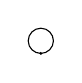
\begin{tikzpicture}[scale=0.4,
 baseline=-0.5ex]
\draw (0,0) circle (0.4);
\fill (0,-0.4) circle (0.05);
\end{tikzpicture}}}$
on $\overline{\mathcal{M}}_{1,1}$ extracts
$\kappaChHodge(\mathrm{Vir}_c) = c/2$ from the subleading pole of
$r^{\mathrm{Vir}}(z)$. The leading pole $(c/2)/z^3$
contributes zero after the $\operatorname{Res}_{z=0}$
extraction (no $z^{-1}$ term); the subleading pole $2T/z$
contributes
$\operatorname{Res}_{z=0}\,2T/z\,dz = 2\langle T \rangle
= c/12$. The sewing integral over
$\overline{\mathcal{M}}_{1,1}$ couples this to
$\lambda_1 = 1/24$, giving
$F_1(\mathrm{Vir}_c)=\kappaChHodge(\mathrm{Vir}_c)/24 = c/48$.
After ghost subtraction:
$F_1^{\mathrm{eff}} = \kappa_{\mathrm{eff}}/24 = (c-26)/48$.

The scalar holomorphic seed for the conjectural BTZ bridge is the
exponential of the all-genus generating function
$\sum_{g \ge 1} F_g^{\mathrm{eff}}\,x^{2g}
= \frac{c-26}{2}\bigl(\hat{A}(ix) - 1\bigr)$,
where $\hat{A}(x) = (x/2)/\sinh(x/2)$. The Cardy entropy
$S_{\mathrm{Cardy}} =
2\pi\sqrt{c\Delta_+/6} + 2\pi\sqrt{c\Delta_-/6}$
at large shifted conformal energy is Conjecture~\ref{conj:gravity-cardy}.
It requires the physical torus partition function, its modular
$S$-transform, vacuum dominance, and the saddle-point inversion.
The $r$-matrix is the genus-$0$, degree-$2$ datum that seeds the
scalar tower; the Cardy entropy is a conjectural high-temperature
interpretation of that seed after the analytic inputs are added.

\subsubsection*{Conical defects and BTZ from braiding}

Primitivity of $\Delta_z^{\mathrm{grav}}$ states that the BTZ
spectrum is not built by splitting gravitons. Black holes
form by a different mechanism: accumulation of $r$-matrix
twists. The BTZ black hole of mass $M$ and angular
momentum $J$ is a quotient of AdS$_3$ by a discrete isometry;
its boundary character seed is modeled as a trace over a single
Virasoro module. Identifying that seed with the physical BTZ
partition function again requires the Cardy/BTZ analytic hypotheses,
not a sum over multi-graviton states.
Conical defects of angular deficit $2\pi(1 - \sqrt{1 - 8G_Nh})$
are read as highest-weight modules $M_h$ of the Koszul dual
$\mathrm{Vir}_{26-c}$: they are topological objects, classified by the
monodromy of the $r$-matrix braiding. After the concrete line-side
comparison is fixed, the fusion of two conical defects is expected to
be controlled by four-point conformal blocks of
$\mathrm{Vir}_{26-c}$ and the corresponding Ponsot--Teschner kernel
$\mathbb{F}_{\alpha_s}^{\alpha_t}$ with its external data
(\S\ref{subsec:gravity-r-matrix}). The gravitational $S$-matrix is then
a pure braiding matrix:
it rearranges line operators but never creates new ones.

This is the algebraic content of the classical observation that
three-dimensional gravity is topological. The Einstein--Hilbert
action in three dimensions is equivalent to Chern--Simons theory
for $SL(2,\mathbf{R}) \times SL(2,\mathbf{R})$, and the phase
space consists of flat connections modulo gauge: a
finite-dimensional moduli space with no local excitations. The
Koszul-dual formulation makes this precise. The coproduct
$\Delta_z$ would create local excitations
(propagating gravitons). Its vanishing states that the only
gravitational degrees of freedom are topological:
conical deficits, black holes, and
the modular data encoded in the braiding of line operators.
The $r$-matrix is the complete repository of this
topological content.

\subsubsection*{The $\mathcal{W}_N$ extension and
 non-principal reductions}
\label{par:wn-ghost-obstruction}
\index{W-algebra@$\mathcal{W}$-algebra!ghost-number obstruction}

Theorem~\ref{thm:gravitational-primitivity} applies to principal DS
reductions, including $\mathcal{W}_N$-gravity
($\mathfrak{g} = \mathfrak{sl}_N$) and the M5 brane
($\mathfrak{g} = \mathfrak{gl}_K$), exactly on the ghost-defect
surface stated in the theorem. The essential input is not merely the
slogan \(\mathrm{gh}(h)=-1\), but the signed HPL tree count together
with the projection to ghost-number-zero cohomology.

The DS reduction of $\widehat{\mathfrak{sl}}_N$ by the
principal nilpotent $f = \sum_{i=1}^{N-1} E_{i+1,\,i}$
produces $N(N-1)/2$ ghost pairs
$(b_\alpha, c_\alpha)$ indexed by positive roots
$\alpha \in \Phi^+(\mathfrak{sl}_N)$. The
$\operatorname{ad}(h_0)$-eigenvalue of each root is
its Dynkin grade $j(\alpha) \in \{1, 2, \ldots, N-1\}$.
The conformal weights of the ghost pair at grade~$j$ are
$(1-j,\, j)$, so higher-grade ghost pairs have higher
conformal weight. The ghost number, however, is always
$\mathrm{gh}(b_\alpha) = -1$, $\mathrm{gh}(c_\alpha) = +1$,
regardless of the grade. The Dynkin grade controls the
conformal weight of the intermediate state but has no effect
on the ghost-number argument: every acyclic pair is separated
by exactly one unit of ghost number, and every contraction
by $h_N$ lowers ghost number by exactly~$1$.

After the signed tree count has been verified, the proof of
Theorem~\ref{thm:gravitational-primitivity} applies to the chosen
\(\mathcal W_N\)-generators: the spin-$s$ generators \(W_s\)
(\(s=2,\ldots,N\)) are represented by BRST-closed ghost-zero classes,
\(i_\infty(W_s)=i(W_s)\) on the chosen representatives, and every
nonlinear coproduct tree whose tensor ghost bidegree is not \((0,0)\)
vanishes after projection. This is the higher-spin version of the
Virasoro generator statement, not an ordinary Hopf-primitivity formula
for arbitrary composites.

\begin{remark}[Non-principal nilpotents]
\label{rem:non-principal-ghost}
\index{Drinfeld--Sokolov reduction!non-principal}
For a non-principal nilpotent $f$ in $\mathfrak{g}$, the BRST
complex $C^{\mathrm{DS}}(\mathfrak{g}, f)$ has ghost pairs
$(b_\alpha, c_\alpha)$ indexed by positive roots with
$\langle \alpha, h_0 \rangle > 0$, where $h_0$ is the neutral
element of the $\mathfrak{sl}_2$-triple of~$f$. The homotopy
$h_f$ still has ghost-number degree~$-1$: every acyclic pair
in the Chevalley--Eilenberg complex of $\mathfrak{n}_+(f)$
is separated by one unit of ghost number. Thus the
ghost-number obstruction kills those \emph{nonlinear} HPL
corrections whose signed tree bidegree is not \((0,0)\):
\(\Delta_{z,n}^{\mathcal{W}(\mathfrak{g},f)}(x)=0\) for a chosen
generator \(x\) and \(n\ge2\) only on that ghost-defect surface.
This is the condition to check for hook-type, subregular, and minimal
nilpotents. However, the
\emph{linear} transferred coproduct $\Delta_{z,1}$ requires a
separate argument: for non-principal reductions whose
$\mathcal{W}$-algebra retains weight-$1$ generators (e.g.\
the Bershadsky--Polyakov algebra from $(\mathfrak{sl}_3,
f_{(2,1)})$, which has an $\widehat{\mathfrak{sl}}_2$
subalgebra at weight~$1$), the projection~$p$ does not
automatically kill the split Casimir cross-terms. The
resolution (Remark~\ref{rem:bp-coproduct-resolved}) is that
\emph{generator}-primitivity holds (the ghost-number
obstruction kills all cross-terms on free generators), but
\emph{composite}-primitivity can fail: fields built from
surviving weight-$1$ generators (e.g.\ the Sugawara stress
tensor) may acquire cross-terms from the split Casimir.
\end{remark}

\begin{remark}[BP coproduct: resolved]
\label{rem:bp-coproduct-resolved}
\index{Bershadsky--Polyakov algebra!coproduct resolution}
The linear transferred coproduct $\Delta_{z,1}$ \emph{is}
primitive for the Bershadsky--Polyakov algebra
$\mathcal{W}(\mathfrak{sl}_3, f_{(2,1)})$ on all free
generators, but not on composites. The three free generators
behave as follows:
\begin{enumerate}
\item $G^+ = J^{E_{23}}$ and $G^- = J^{E_{31}}$ are
 fundamental affine generators. Because $E_{23}$ and
 $E_{31}$ are root vectors for simple roots of the
 $\mathfrak{sl}_2$-complement, the split Casimir
 $\Omega = \sum t^a \otimes t_a$ contributes no cross-term
 of the form $J^{E_{23}} \otimes (\cdots)$ or vice versa:
 the Casimir component $E_{23} \otimes E_{32}$ pairs a
 surviving direction with a BRST-exact one. Thus
 $\Delta_{z,1}(G^\pm) = G^\pm \otimes 1 + 1 \otimes G^\pm$.
\item The weight-$1$ generator $J$ involves Cartan currents
 and ghost bilinears. Ghost cross-terms are killed by the
 ghost-number projection $p \otimes p$: any term with
 nonzero ghost number in either tensor factor vanishes
 under projection to the ghost-number-zero summand.
 Thus $\Delta_{z,1}(J) = J \otimes 1 + 1 \otimes J$.
\item The stress tensor $T$ is a \emph{composite} (Sugawara
 plus ghost corrections), not a free generator. Its
 coproduct is \emph{non-primitive}: the $\mathfrak{sl}_3$
 Casimir has a surviving Cartan component
 $H_1 \otimes H_1$ that projects to $J \otimes J$ under
 $p \otimes p$, giving a nonzero cross-term
 $\Delta_{z,1}(T) \ni (1/z)\, J \otimes J$.
\end{enumerate}
The dichotomy between principal and
non-principal DS reductions is sharp:
\begin{itemize}
\item \textbf{Principal} ($\mathrm{Vir}$, $\mathcal{W}_N$):
 the chosen ghost-zero generators are primitive on the ghost-defect
 surface. Since no weight-$1$ generators survive the reduction, the
 linear split-Casimir obstruction for the stress-tensor generator is
 absent; composites are still read through the \(\Ainf\)-morphism
 identities.
\item \textbf{Non-principal} (Bershadsky--Polyakov and its
 generalisations): free generators are primitive, but
 composites built from surviving weight-$1$ fields are
 non-primitive. The surviving weight-$1$ Casimir component
 provides exactly the cross-terms that escape the
 ghost-number filter.
\end{itemize}
The gap flagged in Remark~\ref{rem:non-principal-ghost} is resolved
only at the stated generator level: primitivity holds on the free
generators after the projection checks above, while the composite
non-primitivity is a \emph{consequence} of the Sugawara construction
and does not obstruct the HPL transfer.
\end{remark}

\begin{remark}[Scope and the infinite tower]
\label{rem:primitivity-scope}
\label{rem:coproduct-gap-closed}
\index{coproduct!scope of primitivity}
Theorem~\ref{thm:gravitational-primitivity} resolves the coproduct
question only after the signed principal-DS ghost-defect lemma has
been verified. What is unconditional here is the mechanism: the total
ghost number
$\mathrm{gh}_{\mathrm{tot}} = \sum_\alpha \mathrm{gh}(c_\alpha)$
is a global $\mathbb{Z}$-grading regardless of the number of ghost
pairs, the homotopy~$h_f$ has $\mathrm{gh}(h_f) = -1$ for
structural reasons (forced by the SDR equation
$\pi \circ h = 0$, $h \circ \iota = 0$, $h^2 = 0$),
and $p \otimes p$ kills every tensor component whose bidegree is not
\((0,0)\). The remaining coproduct obligation is precisely
Remark~\ref{rem:principal-ds-ghost-defect-obligation}: prove that all
nonlinear HPL coproduct trees on the chosen principal generators have
such nonzero tensor ghost bidegree. The gaps of
Remark~\ref{rem:ds-hpl-honest-gaps} concern the transferred
\(\Ainf\) products and the dg-shifted Yangian axioms. The infinite
complexity of
class~$\mathbf{M}$ algebras ($\mathrm{Vir}$,
$\mathcal{W}_N$ for all $N$) resides entirely in the
transferred products $\{m_n^W\}_{n \ge 3}$ and the
$r(z)$-twisted target product once the generator-level coproduct
strictification is installed.
\end{remark}

%====================================================================
% THE GENUS TOWER
%====================================================================

\subsection{The genus tower}
\label{subsec:gravity-genus-tower}

At genus~$0$ the $\Ainf$ tower, the Koszul triangle, the
$R$-matrix, and the coproduct live on
$\FM_k(\C) \times \Conf_k^<(\R)$, the product of holomorphic
and topological configuration spaces on $\C \times \R$. The
curvature $d_{\mathrm{fib}}^2 = \kappa_{\mathrm{eff}}
\cdot \omega_g$ measures the failure of the genus-$0$
differential to square to zero on genus-$g$ surfaces,
and the genus tower $\{F_g\}_{g \ge 1}$ records this
failure as a sequence of Hodge integrals.

\subsubsection*{Genus-$1$ curvature}

The effective gravitational curvature
(Remark~\ref{rem:gravity-kappa-vs-kappa-eff}) is
\begin{equation}\label{eq:gravity-kappa}
\kappa_{\mathrm{eff}}
\;=\;
\frac{c - 26}{2}
\;=\;
3k - 13.
\end{equation}
The bar differential at genus~$1$ acquires curvature
$d_{\mathrm{fib}}^2 = \kappa_{\mathrm{eff}} \cdot \omega_1$
from the self-loop graph on $\overline{\cM}_{1,1}$. The genus-$1$
free energy:
\begin{equation}\label{eq:gravity-F1}
F_1(\mathrm{Vir}_c)
\;=\;
\kappa_{\mathrm{eff}} \cdot \frac{1}{24}
\;=\;
\frac{c - 26}{48}.
\end{equation}
The corresponding $\eta$-function factor packages the
genus-$1$ oscillator contribution as a function of~$\tau$; it
is distinct from the constant free energy~$F_1$.
Here $\eta(\tau) = q^{1/24}\prod_{n \ge 1}(1 - q^n)$.

\begin{remark}[Intrinsic vs.\ effective free energy at genus $1$]
\label{rem:gravity-F1-intrinsic-vs-effective}
The \emph{intrinsic} genus-$1$ free energy of $\mathrm{Vir}_c$ is
$F_1^{\mathrm{intr}} = \kappaChHodge(\mathrm{Vir}_c)/24 = c/48$,
using the intrinsic modular characteristic $\kappa = c/2$
(see Computation~\ref{comp:genus1-free-energy}).
The \emph{effective} value $F_1^{\mathrm{eff}} = (c-26)/48$
in~\eqref{eq:gravity-F1} is the physical quantity after
ghost subtraction ($\kappa_{\mathrm{ghost}} = -13$). At
$c = 26$: $F_1^{\mathrm{eff}} = 0$. This is genus-one ghost
cancellation; it does not truncate the higher-genus scalar series nor
the Virasoro $\Ainf$ tower.
The corresponding determinant-line oscillator shadows on a torus~$E_\tau$
are $Z_1^{\mathrm{intr}}(\tau) = \eta(\tau)^{-c/2}$ and
$Z_1^{\mathrm{eff}}(\tau) = \eta(\tau)^{-(c-26)/2}$.
\end{remark}

\subsubsection*{All genera: the $\hat A$-genus and the Wick rotation}

The genus-$g$ effective scalar free energy is
\[
F_g^{\mathrm{eff}}(\mathrm{Vir}_c \otimes bc_2)
= \kappaChHodge(\mathrm{Vir}_c \otimes bc_2)
  \lambda_g^{\mathrm{FP}}
= \kappa_{\mathrm{eff}}\lambda_g^{\mathrm{FP}},
\]
where
$\lambda_g^{\mathrm{FP}}
=\int_{\overline{\cM}_{g,1}}\psi_1^{2g-2}\lambda_g$,
with generating function
\begin{equation}\label{eq:gravity-generating}
\sum_{g \ge 1} F_g\,x^{2g}
\;=\;
\frac{c - 26}{2}\bigl(\hat{A}(ix) - 1\bigr),
\qquad
\hat{A}(x) = \frac{x/2}{\sinh(x/2)}.
\end{equation}
The argument~$ix$, not~$x$, is the content.
The $\hat{A}$-genus
$\hat{A}(x) = (x/2)/\sinh(x/2)$
is the characteristic series of the Dirac index:
its Taylor coefficients are the alternating Bernoulli
numbers.
The substitution $x \mapsto ix$ converts
$\sinh(ix/2) = i\sin(x/2)$, producing
$\hat{A}(ix) = (x/2)/\sin(x/2)$
with all coefficients positive.
This is the Wick rotation
from Lorentzian (oscillatory Dirac index, alternating signs)
to Euclidean (convergent Hodge integrals, definite signs):
the factor $i^{2g} = (-1)^g$ on each monomial~$x^{2g}$
absorbs the alternation. The individual coefficients
are the Faber--Pandharipande Hodge integrals
$\int_{\overline{\cM}_{g,1}}\psi_1^{2g-2}\lambda_g
= \frac{2^{2g-1}-1}{2^{2g-1}} \cdot \frac{|B_{2g}|}{(2g)!}
=: \lambda_g^{\mathrm{FP}} > 0$
for all $g \ge 1$, and their generating function is
$\hat{A}(x) = (x/2)\operatorname{csch}(x/2)$.
The prefactor $\kappa_{\mathrm{eff}} = (c{-}26)/2$ is the
single datum from the boundary algebra after ghost
subtraction.\label{obs:genus-tower-wick-anomaly}%
\index{Wick rotation!anomaly interpretation}%
\index{genus tower!as Wick rotation anomaly}%

Since every $\lambda_g^{\mathrm{FP}}$ is positive,
the genus tower has uniform sign
$\operatorname{sgn}(\kappa_{\mathrm{eff}})$
at every genus: subcritical ($c < 26$) gives
$F_g < 0$ for all~$g$;
supercritical ($c > 26$) gives $F_g > 0$;
critical ($c = 26$) gives $F_g = 0$.
No sign alternation survives the Wick rotation.

\begin{remark}[Why the $\hat{A}$-genus]
\label{rem:why-A-hat-genus}
\index{A-hat genus@$\hat{A}$-genus!why it appears}%
Three independent routes force $\hat{A}$ rather than the Todd class:
\begin{enumerate}
\item \emph{Symmetry.} The genus tower uses only even powers of~$x$.
 The Todd class $\mathrm{Td}(x) = x/(1-e^{-x})$ has odd powers.
 The product $\mathrm{Td}(x)\cdot\mathrm{Td}(-x)
 = x^2/((1-e^{-x})(e^x-1)) = x^2/(4\sinh^2(x/2))$ is even;
 its positive square root $x/(2\sinh(x/2)) = \hat{A}(x)$.
\item \emph{KO orientation.} The Hodge bundle $\mathbb{E}$ on
 $\overline{\mathcal{M}}_g$ carries a real structure via Serre
 duality ($\mathbb{E}^* \simeq \mathbb{E} \otimes \omega$).
 Real vector bundles are oriented by KO-theory, whose
 multiplicative genus is the $\hat{A}$-genus. Complex vector
 bundles would give the Todd class via KU-theory.
\item \emph{Explicit integration.} The Faber--Pandharipande
 integral
 $\lambda_g^{\mathrm{FP}}
 = \frac{2^{2g-1}-1}{2^{2g-1}} \cdot \frac{|B_{2g}|}{(2g)!}$
 equals the coefficient of $x^{2g}$ in
 $\hat{A}(ix) - 1 = (x/2)/\sin(x/2) - 1$
 (the standard Mittag-Leffler expansion
 $z/\sin(z) = 1 + 2\sum_{g \ge 1}
 \tfrac{(2^{2g-1}-1)|B_{2g}|}{(2g)!}\,z^{2g}$
 identifies the Taylor coefficients with
 $\lambda_g^{\mathrm{FP}}$; verified numerically through
 $g = 6$). The factor
 $(2^{2g-1}-1)/2^{2g-1}$ arises from the boundary-strata
 decomposition $\csc(u) = \cot(u) + \tan(u/2)$.
\end{enumerate}
\end{remark}

\medskip

The vanishing locus $\kappa_{\mathrm{eff}} = 0$ admits
a modular reading.
The genus-$1$ partition function
$Z_1^{\mathrm{eff}}(\tau) = \eta(\tau)^{-\kappa_{\mathrm{eff}}}$
transforms under the modular $S$-transform
$\tau \mapsto -1/\tau$ with weight $-\kappa_{\mathrm{eff}}/2$,
because $\eta(-1/\tau) = \sqrt{-i\tau}\cdot\eta(\tau)$.
At $\kappa_{\mathrm{eff}} = 0$ the scalar modular weight vanishes:
$c = 26$ is the unique central charge at which
$Z_1^{\mathrm{eff}}$ is $S$-invariant.
The genus tower therefore measures the scalar anomaly:
$F_g \ne 0$ at genus~$g$ is the $g$-th
anomaly coefficient. The Cardy entropy
$S_{\mathrm{Cardy}} =
2\pi\sqrt{c\Delta_+/6} + 2\pi\sqrt{c\Delta_-/6}$
\textup{(}Conjecture~\textup{\ref{conj:gravity-cardy})}
is a physical high-temperature extraction only after the full modular
partition function, vacuum dominance, and saddle-point approximation
are supplied.
The single chain
\[
\text{quartic pole}
\;\longrightarrow\;
\kappa
\;\longrightarrow\;
d_{\mathrm{fib}}^2 = \kappa_{\mathrm{eff}}\cdot\omega_g
\;\longrightarrow\;
F_g \ne 0
\;\xrightarrow{\text{physical hypotheses}}\;
S_{\mathrm{Cardy}}
\]
separates the proved OPE-to-scalar tower from the conjectural entropy
extraction.

\begin{remark}[Modularity from the open sector]
\label{rem:gravity-modularity-open-sector}
\index{modularity!from open sector}
The genus tower is not an axiom on the closed algebra
$\mathrm{Vir}_c$. It arises from trace and clutching on the
gravitational open-sector factorization dg-category
$\cC_{\mathrm{grav}}^{\mathrm{op}}$
\textup{(}Definition~\textup{\ref{def:grav-open-category})}: the
annulus trace $\int_{S^1} \cC_{\mathrm{grav}}^{\mathrm{op}}
\simeq \HH^{\mathrm{ch}}_\bullet(\mathrm{Vir}_c)$ is the first modular shadow
\textup{(}\eqref{eq:grav-annulus-trace}\textup{)}, and
clutching along shared boundary circles raises genus. The
scalar $\kappa_{\mathrm{eff}}$ enters as the trace of the
cyclic pairing on $\End(b)$, not as primitive closed-string data.
The MC equation on the bordered FM compactification
$\overline{C}{}^{\,\mathrm{oc}}_{k,\vec{m}}$ packages both
sectors into a single identity whose closed projection recovers
\[
F_g^{\mathrm{eff}}(\mathrm{Vir}_c \otimes bc_2)
= \kappaChHodge(\mathrm{Vir}_c \otimes bc_2)
  \lambda_g^{\mathrm{FP}}.
\]
\end{remark}

\begin{remark}[Gravitational content as closed-sector projection of $\SCchtop$]
\label{rem:gravity-closed-sector-projection-genus}%
\index{3d gravity!closed-sector projection}%
\index{Swiss-cheese operad!gravitational projection}%
Every gravitational quantity in this section is the
$\Sigma_n$-coinvariant (closed-sector) projection of an ordered
$\SCchtop$-structure. The curvature $\kappa_{\mathrm{eff}}$ is
$\mathrm{av}(r(z))$, the image of the classical $r$-matrix
under the averaging map $\mathrm{av}\colon
\mathfrak{g}^{E_1}_{\mathrm{Vir}} \to
\mathfrak{g}^{\mathrm{mod}}_{\mathrm{Vir}}$
(Remark~\ref{rem:e1-colour-primitive}). The free energy
$F_g^{\mathrm{eff}}(\mathrm{Vir}_c \otimes bc_2)
= \kappaChHodge(\mathrm{Vir}_c \otimes bc_2)
\lambda_g^{\mathrm{FP}}$ is the image of the ordered genus-$g$ amplitude. The full ordered
ancestor carries strictly more data: the $R$-matrix, the braided
monoidal structure on line operators, and the conditional
dg-shifted-Yangian completion $\Ydg(\mathrm{Vir}_c)$. The closed-sector
projection discards this data and retains only the scalar
shadow obstruction tower of Volume~I. Three-dimensional quantum
gravity, in the Virasoro $\SCchtop$-algebra formulation, is
the modular shadow of the ordered Virasoro line package; the
Yangian reading is the strictified comparison after the
axioms isolated in Remark~\ref{rem:ds-hpl-honest-gaps} are verified.
\end{remark}

\begin{remark}[Gravitational content as $\Sigma_n$-descent of the $\SCchtop$-structure]
\label{rem:gravity-sigma-descent}%
\index{3d gravity!Sigma-n descent@$\Sigma_n$-descent}%
\index{Swiss-cheese operad!gravitational content}%
The preceding remark identifies every gravitational quantity as
a $\Sigma_n$-coinvariant projection. In the language of the
three-bar-complex hierarchy
(Remark~\ref{rem:sc-three-bar-connection} in
\S\ref{sec:foundations}), the gravitational genus tower
$F_g^{\mathrm{eff}}(\mathrm{Vir}_c \otimes bc_2)
= \kappaChHodge(\mathrm{Vir}_c \otimes bc_2)
\lambda_g^{\mathrm{FP}}$ is an invariant of the symmetric bar $\barBch(\mathrm{Vir}_c)$,
while the full $\SCchtop$-structure of $\mathrm{Vir}_c$
also encodes the $R$-matrix, the braided monoidal
structure on gravitational line operators, and the dg-shifted
Yangian $\Ydg(\mathrm{Vir}_c)$.
The derived center $Z^{\mathrm{der}}_{\mathrm{ch}}(\mathrm{Vir}_c)$
(Volume~I, Theorem~\ref*{V1-thm:thqg-swiss-cheese}) is the
algebraic closed-colour vertex attached to the Virasoro boundary
chart. It is computed by chiral Hochschild cochains of any compact
boundary chart, not by the bar complex.
The bar complex classifies twisting morphisms (couplings between
$\mathrm{Vir}_c$ and $\mathrm{Vir}_{26-c}$). Its physical
gravitational reading uses the Virasoro HT prefactorization
realisation, the Brown--Henneaux boundary chart
\(c=3\ell/(2G_N)\), and the \(\Sigma_n\)-closed-sector descent.
In pure 3d gravity this reading further passes to the
central-extension quotient \(\C[\![c]\!]\) of
Theorem~\ref{thm:gravity-koszul-triangle}. Thus three-dimensional
gravity reads the central scalar shadow of the full open/closed
$\SCchtop$-structure on the Virasoro algebra; it is not the whole
derived centre.
\end{remark}

\begin{remark}[Bi-based factorisation datum at the K3$\times T^2$
compactification]
\label{rem:3dqg-bi-based-factorisation}%
\index{factorisation datum!bi-based!K3$\times T^2$}%
\index{Kodaira fibre!24 nearby cycles}%
\index{SC@$\SCchtop$!K3 specialisation}%
The closed-sector projection of the Virasoro $\SCchtop$-structure
admits a geometric refinement at the K3$\times T^2$ compactification
relevant to the 3d-gravity climax. In this frame the ordered
ancestor is a \emph{bi-based factorisation datum}: a chiral
factorisation algebra on the Ran space
$\mathrm{Ran}(E^{\mathrm{nod},\mathrm{sm}}_{24})$ of the elliptic
K3 with $24$ Kodaira I$_1$ nodal points attached together with a
parameter factorisation on the compactified genus-$2$ Siegel moduli
space $\overline{\cA}_2$. The bi-based structure is the pair
\[
\bigl(
\mathrm{Fact}^{\mathrm{ch}}_{\mathrm{Ran}(E^{\mathrm{nod},\mathrm{sm}}_{24})}(\mathrm{Vir}_c),
\;
\mathrm{Fact}^{\mathrm{param}}_{\overline{\cA}_2}
\bigr)
\]
linked by the Francis--Gaitsgory $\infty$-categorical pushforward
along the Kuga--Satake correspondence, with nearby-cycles at the
$24$ Kodaira nodes supplying the Costello--Gaiotto 5-brane vertex
data of \cite{CostelloGaiotto2018,Costello2021}. The
$\SCchtop$-structure on the bulk-boundary pair
$\bigl(C^\bullet_{\mathrm{ch}}(\mathrm{Vir}_c,\mathrm{Vir}_c),
\mathrm{Vir}_c\bigr)$ of
Chapter~\ref{ch:sc-chtop-heptagon} specialises to this bi-based
datum, with the averaging map factoring
\[
\mathrm{av}
\;=\;
\mathrm{Torelli}_{\mathrm{K3}}
\,\circ\,
\mathrm{KugaSatake}
\,\circ\,
j_{\mathrm{Kodaira}}
\]
through the Kuga--Satake $\mathbb{Z}/2$-spin cover of $\cA_2$.
Bi-basing the factorisation is the geometric mechanism that
relates the chain-level $\SCchtop$-heptagon
(Theorem~\ref{thm:sc-heptagon}) to the
$(\infty,1)$-categorical bulk-boundary pair of
Part~\ref{part:gravity}: both lanes present the same geometric
object, viewed through different factorisation bases.
Primary literature: \cite{FrancisGaitsgory2012} (parametrised
factorisation $\infty$-categories);
\cite{CostelloGaiotto2018,Costello2021} (twisted M-theory and
5-brane vertex algebra on K3$\times T^2$).
\end{remark}

\subsubsection*{The normalized determinant-line partition shadow}

The normalized determinant-line partition shadow for the SL$(2,\R) \times$
SL$(2,\R)$ theory (left$+$right) is
\[
Z_{\mathrm{grav}}^{\mathrm{det,norm}}(\tau, \bar\tau)
\;=\;
|\eta(\tau)|^{(c-26)/6}.
\]
The exponent $(c{-}26)/6$ is $\kappa_{\mathrm{eff}}/3$, reflecting
the per-real-degree-of-freedom normalisation of the
SL$(2,\R) \times$ SL$(2,\R)$ one-loop determinant
($\dim_{\R} \mathfrak{sl}_2 = 3$, two copies).
At $c = 26$ ($k = 13/3$):
$Z_{\mathrm{grav}}^{\mathrm{det,norm}} = 1$, reflecting effective scalar
anomaly cancellation rather than triviality of the full coupled
partition function. At $c = 13$ (fixed point of the line-side
comparison):
$Z_{\mathrm{grav}}^{\mathrm{det,norm}} = |\eta(\tau)|^{-13/6}$.

\subsubsection*{The shadow obstruction tower}

The genus tower is controlled by a sequence of invariants,
each extracted from the $\Ainf$ tower at increasing degree.
The first four named shadows and their gravitational readings:

\begin{center}
\small
\renewcommand{\arraystretch}{1.15}
\begin{tabular}{lll}
\textbf{Shadow} & \textbf{Algebraic origin (Vol~I)} & \textbf{Gravitational counterpart} \\
\hline
$\kappa_{\mathrm{eff}} = (c-26)/2$
 & effective curvature after ghost subtraction
 & one-loop Weyl anomaly; $= 0$ iff $c = 26$ \\[2pt]
$\mathfrak{C}(\mathrm{Vir}_c) = -c$
 & cubic shadow (Vol~I)
 & cubic graviton vertex; $\propto \ell/(16\pi G_N)$ at Brown--Henneaux \\[2pt]
$\mathfrak{Q} = 10/[c(5c+22)]$
 & quartic contact shadow (Computation~\ref{comp:gravity-quartic-correction})
 & genus-$2$ correction $F_2^{\mathrm{contact}}$ \\[2pt]
$o_5 \ne 0$
 & quintic obstruction (Vol~I, non-vanishing)
 & genus-$2$ five-point contribution to $F_2$
\end{tabular}
\end{center}

The shadow obstruction tower does not terminate
(by the explicit Virasoro quartic-contact computation of Volume~I):
the $r$-th shadow determines the $r$-graviton
vertex, and no finite
truncation determines the full perturbative hierarchy.

\begin{computation}[Quartic contact shadow and genus-$2$ contact
correction]
\label{comp:gravity-quartic-correction}%
\index{quartic contact shadow!genus-2 contact correction}%
The quartic contact shadow
$\mathfrak{Q}^{\mathrm{contact}}_{\mathrm{Vir}} = 10/[c(5c+22)]$
from the quartic-contact analysis of Volume~I
determines the genus-$2$ contact correction
$F_2^{\mathrm{contact}}$, the
leading nonlinear partition-function correction beyond the
one-loop sector.

\emph{Explicit evaluation.} At the Brown--Henneaux chiral central
charge $c = 6k = 3\ell/(2G_N)$:
\begin{alignat*}{2}
\mathfrak{Q}(c = 6k)
\;&=\;
\frac{10}{6k(30k+22)}
\;=\;
\frac{5}{6k(15k+11)},
\\[4pt]
\intertext{and the genus-$1$ Hessian correction
$\delta_H^{(1)} = 120/[c^2(5c+22)]$ evaluates to}
\delta_H^{(1)}(c = 6k)
\;&=\;
\frac{120}{36k^2(30k+22)}
\;=\;
\frac{5}{3k^2(15k+11)}.
\end{alignat*}
In the semiclassical limit $k \to \infty$ (equivalently
$G_N \to 0$):
\[
\mathfrak{Q} \;\sim\; \frac{1}{18k^2},
\qquad
\delta_H^{(1)} \;\sim\; \frac{1}{9k^3}.
\]
The quartic correction enters the genus-$2$ partition function
through marked contact classes, not through an unmarked
$\psi$-integral on $\overline{\cM}_2$.  The unmarked genus-$2$
curvature class is
\[
  \Omega_2^{\mathrm{curv}}=\kappa\,\lambda_2
  \in R^2(\overline{\cM}_2),
\]
and becomes a number only after pairing with a complementary socle
class:
\[
  \int_{\overline{\cM}_2}\kappa\,\lambda_2\lambda_1
  =
  \frac{\kappa}{5760}
  =
  \frac{c}{11520}.
\]
On the one-marked space the Faber--Pandharipande Hodge integral is
\[
  \int_{\overline{\cM}_{2,1}}\psi_1^2\lambda_2
  =
  \frac{7}{5760},
  \qquad
  F_{2,1}^{\mathrm{FP}}=\frac{7c}{11520},
\]
while the pure psi-class integral is
\[
  \int_{\overline{\cM}_{2,1}}\psi_1^4=\frac{1}{1152}.
\]
Thus any scalar genus-$2$ contact coefficient must specify whether it
uses the pure psi class or the Hodge-weighted class.  The symbol
$\mathfrak Q=10/[c(5c+22)]$ supplies the Virasoro contact coupling;
the tautological integral supplying the genus-$2$ number is separate
data.

\emph{Gravitational interpretation.}
The quartic shadow $\mathfrak{Q}$ is read as the four-graviton
contact coupling: a connected genus-$0$ amplitude with four external
stress-tensor insertions, exchanged through the one-loop wheel
graph $C_4$. Its nonvanishing ($\mathfrak{Q} \neq 0$ for
$c \neq 0$) is the algebraic witness that $3$d gravity has genuine
nonlinear dynamics beyond one loop,
and the non-terminating support packet
\(r^\Theta_{\max}(\mathrm{Vir}_c)=\infty\)
(class~M, in the completed ambient) is read as meaning that the
algebraic graviton interaction tower has no finite support cutoff.

\emph{Complementarity.} Under the same-family Virasoro shadow
$c \mapsto 26 - c$:
\[
\mathfrak{Q}(c) + \mathfrak{Q}(26-c)
\;=\;
\frac{10}{c(5c+22)} + \frac{10}{(26-c)(152-5c)}.
\]
At $c = 13$ (self-dual): $\mathfrak{Q}(13) = 10/(13 \cdot 87) =
10/1131$. The complementarity of the quartic shadow across the
Koszul involution is
the first nonlinear witness of the duality between boundary and
line sectors.
\end{computation}

%====================================================================
% THREE-DIMENSIONAL GRAVITY
%====================================================================

\subsection{The physics of 3d gravity}
\label{subsec:gravity-physics}

Everything above was derived from the $\lambda$-bracket
$\{T_\lambda T\} = \partial T + 2T\lambda + (c/12)\lambda^3$.
The following shows that, via the physics-bridge theorem and the
Chern--Simons realization, this algebraic package recovers the
three-dimensional Einstein-gravity package with
$\Lambda = -1/\ell^2$.

\subsubsection*{The Chern--Simons origin}

Three-dimensional gravity with $\Lambda < 0$ is equivalent to
$SL(2,\R) \times SL(2,\R)$ Chern--Simons at level
$k = \ell/(4G_N)$.  For one oriented chiral factor the
Brown--Henneaux boundary central charge is
$c_{\mathrm{ch}} = 6k = 3\ell/(2G_N)$
\cite{BrownHenneaux,Witten88}. The dreibein $e^a$ and spin
connection $\omega^a$ combine into $A_\pm = \omega \pm e/\ell$;
flat connections $F_\pm = 0$ are constant-curvature geometries.

\begin{theorem}[Brown--Henneaux chiral boundary chart;
\ClaimStatusProvedElsewhere; licensing $\alpha+\beta+\gamma$
via $\hypBHdict$]
\label{thm:brown-henneaux}
\index{Brown--Henneaux central charge|textbf}
Under Brown--Henneaux asymptotic boundary conditions for Lorentzian
AdS$_3$ Einstein gravity with \(\Lambda=-1/\ell^2\), the canonical
boundary charge algebra of one oriented $SL(2,\R)$ Chern--Simons
factor at level \(k=\ell/(4G_N)\) is
\(\mathrm{Vir}_{c_{\mathrm{ch}}}\), with
\[
c_{\mathrm{ch}} = 6k = \frac{3\ell}{2G_N}.
\]
Full AdS$_3$ gravity has the two oriented chiral factors
$SL(2,\R)_+\times SL(2,\R)_-$ and hence two commuting Virasoro
copies, one for each boundary orientation.  This is the external
asymptotic-symmetry/Chern--Simons comparison theorem
\cite{BrownHenneaux,Witten88}; it is not a theorem of the bar complex.
\end{theorem}

\begin{proof}
Brown--Henneaux compute the canonical boundary charges for the
AdS$_3$ asymptotic boundary condition and obtain a Virasoro central
extension.  In the Chern--Simons presentation of Witten, one chiral
factor may be put in Drinfeld--Sokolov boundary gauge
\[
A_z|_{\partial} = J_- + T(z)\,J_+ .
\]
The residual gauge transformation \(g=\exp(\epsilon J_+)\) acts by
$\delta_\epsilon T = \epsilon' T + 2\epsilon T' +
(c/12)\epsilon'''$, the Virasoro coadjoint action with
central charge \(c=6k\).  The Chern--Simons symplectic form induces
the canonical charge Poisson bracket, in the divided-power convention
matching
\eqref{eq:gravity-input},
$\{T(z), T(w)\}_{\mathrm{PB}} = (c/12)\partial_w^3\delta(z-w) +
2T(w)\delta'(z-w) + T'(w)\delta(z-w)$,
which is~\eqref{eq:gravity-input} in distribution form.
The present chapter uses this external result only to install the
Brown--Henneaux boundary chart \(b_{\mathrm{BH}}\) with
\(A_{b_{\mathrm{BH}}}=\mathrm{Vir}_{c_{\mathrm{ch}}}\).
\end{proof}

\begin{remark}[Brown--Henneaux read through the thesis]
\label{rem:brown-henneaux-from-thesis}
\index{Brown--Henneaux central charge!thesis reading}
\index{unifying thesis!Brown--Henneaux reading}
The Brown--Henneaux formula $c = 3\ell/(2G_N)$
(Theorem~\ref{thm:brown-henneaux}) admits a compact reformulation
through the unifying thesis
$A \mapsto \Zder^{\mathrm{ch}}(A)$. For $A = \mathrm{Vir}_c$,
$\kappaChHodge(A) = c/2$, so the combination $2\kappaChHodge(A)$
equals the boundary central charge appearing in
bulk-boundary observables. The dimensional input
$c = 6k$, $k = \ell/(4G_N)$ is the Ach\'ucarro--Townsend--Witten
Chern--Simons presentation of 3d gravity and is taken from
that source, not derived from the bar complex; the thesis
does not produce the coupling to $G_N$ on its own. What the thesis
does deliver is a uniform re-expression of the scalar genus tower as a
\(\kappa\)-polynomial, together with the \(\kappa=c/2\) input that a
physical Brown--Henneaux/Cardy/BTZ comparison would use. Cardy
degeneracy and BTZ entropy are not obtained from the bar complex
without modular invariance, vacuum dominance, and saddle extraction.
In particular, this remark is
\emph{not} a derivation of Brown--Henneaux from Koszul duality;
it is an interface observation that collects the chiral
curvature $\kappa$ and the physics constant $c = 3\ell/(2G_N)$
into a single notational track.
\end{remark}

\begin{remark}[Brown--Henneaux through the thesis lens]
\label{rem:brown-henneaux-thesis}
Brown--Henneaux is a semiclassical theorem
(Theorem~\ref{thm:brown-henneaux}): a classical calculation
on $SL(2,\R)$ Chern--Simons produces the Virasoro charge with
$c = 3\ell/(2G_N)$. The thesis does not supplant that
calculation; it reorganizes the invariants. With
$\kappaChHodge(\mathrm{Vir}_c) = c/2$ the boundary central charge
tracks the chiral curvature, so that once Brown--Henneaux
has fixed $c$ in terms of $\ell/G_N$ the rest of the
holographic dictionary is parametrized by the single scalar
$\kappa$. The thesis supplies a uniform language for the
bar-complex consequences of that value; it does not derive
the Brown--Henneaux value itself.
\end{remark}

\subsubsection*{Physics-bridge verification for gravity}

\begin{theorem}[Brown--Henneaux Virasoro MC bridge;
\ClaimStatusConditional; licensing
$\alpha+\beta+\gamma+\delta+\varepsilon$
via $\hypBHdict+\hypAmbientWtCpl+\effKoszul$]
\label{thm:gravity-mc}
\index{universal MC element!3d!gravitational}
Fix one oriented Brown--Henneaux chiral factor
\(b_{\mathrm{BH}}\) at level \(k=\ell/(4G_N)\), with
\(A_{b_{\mathrm{BH}}}=\mathrm{Vir}_{c_{\mathrm{ch}}}\) and
\(c_{\mathrm{ch}}=6k=3\ell/(2G_N)\).  Assume the corresponding
Chern--Simons BV model with boundary condition \(b_{\mathrm{BH}}\)
satisfies the product HT hypotheses of
Theorem~\ref{thm:physics-bridge} \textup{(}BV datum, factorized
logarithmic parametrix, one-loop finiteness, and product-polynomial
interactions\textup{)}, work in the completed ambient
\(\hypAmbientWtCpl\), and impose the chirally Koszul line-side
effectiveness condition \(\effKoszul\).  Then the resulting logarithmic
\(\SCchtop\)-algebra determines a homotopy Maurer--Cartan package
\[
\alpha_{\mathrm{grav}}\in\mc(\gSC_T).
\]
Its licensed projections are:
\begin{enumerate}[label=\textup{(\roman*)}]
\item boundary/chiral face
 \(A_{b_{\mathrm{BH}}}=\mathrm{Vir}_{c_{\mathrm{ch}}}\) with
 the Virasoro bracket~\eqref{eq:gravity-input};
\item open face the completed perturbative line category
 \[
 \widehat{\mathcal C}^{\,b_{\mathrm{BH}},\mathrm{pert}}_{\mathrm{line}}
 \simeq
 \mathcal A^{!}_{\mathrm{line}}\text{-}\mathbf{mod}^{A_\infty}
 \]
 under Theorem~\ref{thm:lines_as_modules};
\item spectral face the abstract open-colour line braiding; after the
 collision-residue comparison its singular classical kernel is
 \(r^{\mathrm{coll}}_{\mathrm{Vir}}(z)=\frac{c_{\mathrm{ch}}/2}{z^3}
 +\frac{2T}{z}\);
\item genus/shadow face the bar-intrinsic Virasoro MC element
 \(\Theta_{\mathrm{Vir}_{c_{\mathrm{ch}}}}\) in the completed
 shadow complex;
\item PVA shadow the Virasoro \(\lambda\)-bracket
 \(\{T_\lambda T\}=\partial T+2T\lambda+(c_{\mathrm{ch}}/12)\lambda^3\).
\end{enumerate}
The closed/bulk vertex associated to this boundary chart is
\(\Zder^{\mathrm{ch}}(\mathrm{Vir}_{c_{\mathrm{ch}}})\) after the
bulk--Hochschild comparison; it is not the boundary Virasoro algebra
itself.  The concrete realization of the open face by
\(\mathrm{Vir}_{26-c_{\mathrm{ch}}}\)-modules, the realization of the
spectral face by the Virasoro fusion kernel, and the reading of BTZ
geometries as MC deformations are not part of this theorem.
\end{theorem}

\begin{proof}
The Brown--Henneaux theorem supplies the boundary chart
\(A_{b_{\mathrm{BH}}}=\mathrm{Vir}_{c_{\mathrm{ch}}}\)
with \(c_{\mathrm{ch}}=6k\).  Theorem~\ref{thm:physics-bridge},
applied with the stated BV datum, factorized parametrix, finiteness,
and product-polynomial interaction hypotheses, supplies a logarithmic
\(\SCchtop\)-algebra.  Its structure map from the bar cooperad of
\(\SCchtop\) to the corresponding endomorphism object is precisely the
homotopy Maurer--Cartan package \(\alpha_{\mathrm{grav}}\).

Projection to the boundary chiral colour gives the Virasoro bracket
\eqref{eq:gravity-input}.  Projection to the open colour, together
with the completed perturbative line-category hypothesis and
\(\effKoszul\), is Theorem~\ref{thm:lines_as_modules}.  Projection to
the ordered two-line collision gives the abstract spectral braiding;
the displayed singular kernel is the collision-residue comparison of
Proposition~\ref{prop:gravity-ybe}.  Projection to the modular shadow
complex gives the bar-intrinsic Virasoro MC element
\(\Theta_{\mathrm{Vir}_{c_{\mathrm{ch}}}}\), whose all-genus MC
property is the construction of Theorem~\ref{thm:gravity-mc-package}.
Taking the classical PVA shadow of the boundary bracket gives the
displayed Virasoro \(\lambda\)-bracket.

The derived closed-sector object is obtained only after applying the
bulk--Hochschild comparison to the boundary algebra; by
Theorem~\ref{thm:bulk_hochschild} this object is
\(\Zder^{\mathrm{ch}}(\mathrm{Vir}_{c_{\mathrm{ch}}})\), not
\(\mathrm{Vir}_{c_{\mathrm{ch}}}\).
\end{proof}

\begin{remark}[Scope: abstract vs.\ concrete line-side identifications]
\label{rem:gravity-mc-scope}
The open face and spectral $R$-matrix in
Theorem~\ref{thm:gravity-mc} are proved only on the theorem's stated
completed Brown--Henneaux/Koszul surface: the line-side package exists
as the completed open-colour \(E_1\)-module category of the ordered
bar complex, and the braiding is its abstract spectral braiding. The
\emph{concrete} identification of this package with highest-weight
$\mathrm{Vir}_{26-c}$-modules and of the braiding with the Virasoro
fusion kernel is conjectural; see
Remark~\ref{rem:gravity-line-virasoro-realization} and
Conjecture~\ref{conj:gravity-line-identification}.
\end{remark}

\subsubsection*{BTZ black holes as candidate MC deformations}

\begin{definition}[Candidate BTZ deformation]
\label{def:btz-deformation}
\index{BTZ black hole!as MC deformation}
After the Brown--Henneaux, Cardy, and BTZ comparison data have been
fixed, a BTZ black hole of mass~$M$ and angular momentum~$J$ is
represented in the algebraic model by a candidate MC deformation
\(\delta\alpha \in \gSC_T\) of \(\alpha_{\mathrm{grav}}\), satisfying
\(D_{\alpha_{\mathrm{grav}}}(\delta\alpha) = 0\), with shifted
cylinder energies
\[
\Delta_\pm := L_0^\pm-\frac{c}{24}
= \frac{M\ell \pm J}{2}.
\]
If $h_\pm$ denote highest weights, then
$h_\pm=\Delta_\pm+c/24$.
\end{definition}

\subsubsection*{The Cardy formula: partition function and modular $S$-transform}

The genus-$1$ MC element $\Theta^{(1)}$ produces the boundary
partition function. Write $q = e^{2\pi i\tau}$ for the modular
parameter of the boundary torus. The categorical trace gives
\begin{equation}\label{eq:gravity-Z1}
Z_1(\tau)
\;=\;
\Tr_{\mathrm{Vir}_c}\!\left(q^{L_0 - c/24}\right)
\;=\;
\frac{q^{-c/24}}{\prod_{n=2}^{\infty}(1-q^n)},
\end{equation}
the product starting at $n = 2$ because $\mathrm{Vir}_c$ has no
weight-$1$ states. The full partition function counting all states
at inverse temperature $\beta = 2\pi\,\mathrm{Im}\,\tau$ is
\begin{equation}\label{eq:gravity-Z-full}
Z(\tau,\bar\tau)
\;=\;
\sum_{h,\bar h}
d(h,\bar h)\,q^{h - c/24}\,\bar q^{\bar h - c/24}.
\end{equation}
If the full physical partition function is modular invariant,
$Z(-1/\tau, -1/\bar\tau) = Z(\tau,\bar\tau)$, and vacuum dominated
in the high-temperature limit, then
\begin{equation}\label{eq:gravity-vacuum-dominance}
Z(\tau,\bar\tau)
\;\sim\;
\exp\!\left(
 \frac{\pi c}{6}\,\mathrm{Im}(-1/\tau)
\right)
\qquad (\mathrm{Im}\,\tau \to 0^+).
\end{equation}
For one chiral sector $Z_1(\tau)$ the exponent is
$\pi c\,\mathrm{Im}(-1/\tau)/12$; the displayed formula is the
diagonal full partition function with $c_L=c_R=c$.
In the bar-complex language, the $S$-transform acts on
$\Theta_{\mathrm{grav}}$ by exchanging the two boundary cycles of
the genus-$1$ bordered FM compactification. This is the algebraic
precursor of modular covariance, not the analytic modular invariance
of the physical torus partition function. Vacuum dominance is the
additional statement that the degree-$0$ component
$\Theta^{(1)}_{n=0} = \kappa\cdot\omega_1$ controls the
exponential growth of states.

\subsubsection*{Saddle-point extraction and the Cardy formula}

The chiral degeneracy $d(\Delta_+)$ at large shifted energy is
extracted by inverse Laplace transform from the one-sector exponent.
The
saddle-point of $f(\tau) = \pi c/(12\tau) + 2\pi\tau\Delta_+$
is at
\begin{equation}\label{eq:gravity-saddle}
\tau_*
\;=\;
i\sqrt{\frac{c}{24\Delta_+}}
\;\approx\;
i\sqrt{\frac{c}{24\Delta_+}}
\qquad (\Delta_+ \gg c),
\end{equation}
giving $f(\tau_*) \approx 2\pi\sqrt{c\Delta_+/6}$.

\begin{conjecture}[Cardy formula from the bar complex]
\label{conj:gravity-cardy}
\label{conj:cardy-mc}
\index{Cardy formula!from bar complex|textbf}
\index{BTZ black hole!Cardy formula}
The asymptotic entropy of the Virasoro bar complex at large
shifted conformal energy is
\begin{equation}\label{eq:gravity-cardy}
\boxed{
S_{\mathrm{Cardy}}
\;=\;
2\pi\sqrt{\frac{c\,\Delta_+}{6}}
\;+\;
2\pi\sqrt{\frac{c\,\Delta_-}{6}}.
}
\end{equation}
This is the logarithmic growth rate of MC deformations
of $\alpha_{\mathrm{grav}}$ at shifted energies
$(\Delta_+,\Delta_-)$.
\end{conjecture}

\begin{remark}[Conditional derivation of the Cardy formula]
\label{rem:cardy-derivation}
The derivation rests on three bar-complex inputs:
\begin{enumerate}[label=(\roman*)]
\item The curvature $\kappaChHodge(\mathrm{Vir}_c) = c/2$ from the
 genus-$1$ self-loop, which determines
 $\Theta^{(1)}_{n=0} = \kappa\cdot\omega_1$ and hence the
 vacuum energy $-c/24$.
\item The analytic modular invariance of $Z(\tau,\bar\tau)$.
 The genus-$1$ MC equation supplies the algebraic covariance
 witness on the bordered FM compactification, but does not by
 itself prove modular invariance of the completed physical
 partition function.
\item The saddle-point at
 $\tau_* = i\sqrt{c/(24\Delta_+)}$~\eqref{eq:gravity-saddle},
 which follows from the analytic structure of the
 $S$-channel expansion.
\end{enumerate}
The curvature datum $\kappa = c/2$ fixes the vacuum-energy term
used in the saddle. It does not prove the analytic modular
invariance, vacuum dominance, or saddle expansion. The Cardy
formula is therefore Conjecture~\ref{conj:gravity-cardy}; the
local algebra supplies its scalar input, not its analytic proof.
\end{remark}

\begin{remark}[Cardy growth rate in $\kappa$-variables]
\label{rem:cardy-thesis}
\index{Cardy formula!kappa variables}
The Cardy growth rate can be rewritten using
$\kappaChHodge(\mathrm{Vir}_c) = c/2$: the saddle contribution
$2\pi\sqrt{c\Delta_+/6}$ is
$2\pi\sqrt{\kappa\Delta_+/3}$. This rewriting is a notational
move, not a derivation: the Cardy formula itself is
Conjecture~\ref{conj:gravity-cardy} at the bar-complex level
(the conditional derivation is recorded in
Remark~\ref{rem:cardy-derivation}, whose analytic step
remains conjectural), and the thesis supplies no independent
input beyond the $\kappa$-identification. What the
$\kappa$-form does record is that any class-$\mathbf{M}$ VOA
admitting a Cardy-type asymptotic under the same conjectural
analytic inputs would produce the analogous growth rate
governed by its own curvature; the specific Virasoro
constants are fixed by Brown--Henneaux
(Theorem~\ref{thm:brown-henneaux}), not by the thesis.
\end{remark}

\subsubsection*{BTZ entropy from the bar complex}

\begin{conjecture}[BTZ entropy]
\label{conj:gravity-btz-entropy}
\index{BTZ black hole!entropy|textbf}
\index{Bekenstein--Hawking entropy!from bar complex}
The Bekenstein--Hawking entropy of the BTZ black hole is
\begin{equation}\label{eq:gravity-btz-entropy}
\boxed{
S_{\mathrm{BTZ}}
\;=\;
\frac{2\pi r_+}{4G_N}
\;=\;
2\pi\sqrt{\frac{c\,\Delta_+}{6}}
\;+\;
2\pi\sqrt{\frac{c\,\Delta_-}{6}},
}
\end{equation}
where $c = 3\ell/(2G_N)$ is the Brown--Henneaux chiral central charge
\textup{(}Theorem~\textup{\ref{thm:brown-henneaux})},
$\Delta_\pm=L_0^\pm-c/24$ are the shifted cylinder energies,
and $r_+$ is the outer horizon radius.
Equivalently, $S_{\mathrm{BTZ}} =
2\pi\sqrt{\kappa\Delta_+/3}
+ 2\pi\sqrt{\kappa\Delta_-/3}$ with $\kappa = c/2$.
\end{conjecture}

\begin{remark}[Conditional derivation of the BTZ entropy]
\label{rem:btz-derivation}
Assuming Conjecture~\ref{conj:gravity-cardy}, substitute
$c = 3\ell/(2G_N)$,
$\Delta_+ = (M\ell+J)/2$,
$\Delta_- = (M\ell-J)/2$ into the Cardy
formula~\eqref{eq:gravity-cardy}:
\begin{align*}
S_{\mathrm{BTZ}}
&\;=\;
2\pi\sqrt{\frac{3\ell}{2G_N}\cdot\frac{M\ell+J}{12}}
\;+\;
2\pi\sqrt{\frac{3\ell}{2G_N}\cdot\frac{M\ell-J}{12}}
\\[4pt]
&\;=\;
\frac{2\pi}{8G_N}\bigl((r_+ + r_-) + (r_+ - r_-)\bigr)
\;=\;
\frac{2\pi r_+}{4G_N}.
\end{align*}
In terms of the horizon radii
$M=(r_+^2+r_-^2)/(8G_N\ell^2)$ and
$J=r_+r_-/(4G_N\ell)$, equivalently
$(r_+\pm r_-)^2=8G_N\ell(M\ell\pm J)$.
Thus the Cardy expression gives the standard
Bekenstein--Hawking formula
$S = 2\pi r_+/(4G_N) = \mathrm{Area}/(4G_N)$ for the
one-dimensional horizon.
\end{remark}

\begin{remark}[BTZ entropy in $\kappa$-variables]
\label{rem:btz-thesis}
\index{BTZ black hole!kappa variables}
Conditional on Conjecture~\ref{conj:gravity-cardy} and on
Brown--Henneaux (Theorem~\ref{thm:brown-henneaux}), the BTZ
entropy can be reassembled in $\kappa$-variables. A BTZ
black hole is represented in the comparison model by a candidate MC
deformation
$\delta\alpha \in \gSC_T$ of $\alpha_{\mathrm{grav}}$
(Definition~\ref{def:btz-deformation}). Substituting
$c = 2\kappaChHodge(\mathrm{Vir}_c)$ and the Brown--Henneaux value
$c = 3\ell/(2G_N)$ into the Cardy weight reproduces the area
law, as worked out in Remark~\ref{rem:btz-derivation}. The
area-law coefficient $1/(4G_N)$ is \emph{not} fixed by the
chiral curvature: it is the Bekenstein--Hawking coefficient,
external to the bar complex, and appears here only because
it was already present in the Brown--Henneaux input. What
the $\kappa$-reformulation does deliver is a notational
alignment between the boundary curvature and the bulk area
law, under the assumption that the Cardy conjecture and
Brown--Henneaux both hold in their usual forms.
\end{remark}

\subsubsection*{Verdier duality and the modular $S$-transform}

The Koszul involution $c \mapsto 26-c$ (Verdier duality
$\mathbb{D}$, Theorem~\ref{thm:gravity-verdier-intertwining})
and the modular $S$-transform $\tau \mapsto -1/\tau$ are
independent operations acting on different aspects of the MC
element.

\begin{proposition}[Formal Verdier--$S$ square for the genus-one shadow;
\ClaimStatusConditional; licensing $\beta+\gamma$ via the Verdier
level-swap comparison and $\hypAmbientWtCpl$]
\label{prop:gravity-D-S-commute}
\index{Verdier duality!modular $S$-transform commutativity}
\index{modular $S$-transform!Verdier commutativity}
Let \(S_{\mathrm{sh}}\) be the pullback by the mapping-class
transformation \(\tau\mapsto -1/\tau\) on the completed genus-one
shadow complex, with the Hodge line and the Dedekind multiplier line
kept in the coefficient system. On this normalized shadow complex the
Verdier level-swap and \(S_{\mathrm{sh}}\) form a commuting square:
\[
S_{\mathrm{sh}} \circ \mathbb{D}
\bigl(\Theta_{\mathrm{Vir}_c}^{(1),\mathrm{sh}}(\tau)\bigr)
\;=\;
\mathbb{D} \circ S_{\mathrm{sh}}
\bigl(\Theta_{\mathrm{Vir}_c}^{(1),\mathrm{sh}}(\tau)\bigr)
\;=\;
\Theta_{\mathrm{Vir}_{26-c}}^{(1),\mathrm{sh}}(-1/\tau).
\]
At degree zero this says
\[
S_{\mathrm{sh}}\mathbb{D}
\left(\frac{c}{2}\omega_1\right)
\;=\;
\mathbb{D}S_{\mathrm{sh}}
\left(\frac{c}{2}\omega_1\right)
\;=\;
\frac{26-c}{2}\,S_{\mathrm{sh}}(\omega_1).
\]
This is a statement about the algebraic genus-one shadow, not about
the physical torus partition function.
\end{proposition}

\begin{proof}
\(\mathbb{D}\) acts on the Virasoro parameter and on the bar
coefficient system:
\[
c\longmapsto 26-c,\qquad
\kappaChHodge(\mathrm{Vir}_c)=c/2
\longmapsto
\kappaChHodge(\mathrm{Vir}_{26-c})=(26-c)/2 .
\]
The map \(S_{\mathrm{sh}}\) acts on the genus-one moduli parameter
and tautological coefficient line. These are independent tensor
factors in the completed genus-one shadow ambient
\(\hypAmbientWtCpl\), so the two pullbacks commute. The first
displayed equality is Theorem~\ref{thm:gravity-verdier-intertwining}(ii)
followed by the pullback \(\tau\mapsto -1/\tau\); the second order
first pulls back the shadow along \(\tau\mapsto -1/\tau\) and then
applies the same Verdier level-swap. The degree-zero formula is the
specialization \(\Theta^{(1)}_{n=0}=(c/2)\omega_1\).

The analytic lift to a torus partition function contains the
Dedekind multiplier and the quasi-modular \(E_2\) anomaly, treated in
Proposition~\ref{prop:genus1-modular-anomaly}. Those data are not
asserted by the present algebraic square.
\end{proof}

After the physical modular-invariance and vacuum-dominance hypotheses
of Conjecture~\ref{conj:gravity-cardy} are imposed, and for
\(0\le c\le 26\) with shifted energy \(\Delta\ge0\), the same formal
square gives the paired scalar Cardy expression
\[
S_{\mathrm{Cardy}}(\mathrm{Vir}_c;\,\Delta)
+ S_{\mathrm{Cardy}}(\mathrm{Vir}_{26-c};\,\Delta)
= 2\pi\sqrt{\frac{c\Delta}{6}}
 + 2\pi\sqrt{\frac{(26-c)\Delta}{6}} .
\]
At the fixed point $c = 13$ of the line-side comparison, the two terms are equal and
the total counting capacity is maximized:
$\sqrt{c} + \sqrt{26-c} \le 2\sqrt{13}$
(by concavity of $\sqrt{\cdot}$). At $c = 26$, the dual
contribution vanishes (the Witt algebra has $c = 0$).
This is the entropic shadow of the scalar complementarity
$\varkappa := \kappa + \kappa' = 13$
(Proposition~\ref{prop:gravity-complementarity-constant}), distinct
from the Trinity ghost-charge conductor
$K(\Vir) := c + c^! = 26 = -c_{\mathrm{ghost}}(\BRST_{\Vir})$; the two
are related by $\varkappa = \varrho_{\Vir}\cdot K$ with
$\varrho_{\Vir} = 1/2$.

\subsubsection*{Anomaly completion}

At genus $g \ge 1$, the MC element acquires anomaly corrections via
the transgression algebra $B_\Theta$ of
Chapter~\ref{app:anomaly-completed-topological-holography}.
The secondary anomaly class
\[
u \;=\; \eta^2 \;=\; \kappa_{\mathrm{eff}} \cdot \omega_g
\;=\; \tfrac{c-26}{2} \cdot \omega_g
\;\in\; H^2(\overline{\mathcal{M}}_g)
\]
controls the genus-$g$ Clifford completion
$\mathfrak{G}_g(B_\Theta)$: for $u \neq 0$
(equivalently $c \neq 26$) the Clifford algebra is
nondegenerate, Morita trivial, and the effective scalar genus tower
$F_g^{\mathrm{eff}}(\mathrm{Vir}_c\otimes bc_2)
= \kappaChHodge(\mathrm{Vir}_c\otimes bc_2)
\lambda_g^{\mathrm{FP}}$ is nontrivial at every
genus. At $c = 26$ the class $u$ vanishes in the effective scalar
model, the Clifford relation
$\{\alpha_i,\beta_j\} = \delta_{ij}\eta^2$ degenerates to
anticommutativity, and the scalar-specialized genus-$g$ completion
degenerates to the exterior algebra
$\Lambda^{2g+1} \otimes B/(\Theta_{\mathrm{eff}}^{\min})$.
This is the Clifford/exterior dichotomy of the effective scalar
model: the distinction between $c \neq 26$ and $c = 26$ is encoded in
whether the single class $u \in H^2(\overline{\mathcal{M}}_g)$
vanishes. It does not by itself identify the full coupled
transgression algebra with this scalar specialization.
The full anomaly-completed MC element
$\hat\alpha_{\mathrm{grav}} \in \mc(\hat\gSC_T)$ packages
the gravitational genus tower into a single object.

\begin{remark}[$\Delta_5$ as the scalar K3 automorphic shadow]
\label{rem:3dqg-delta5-11d-sugra}%
\index{11D supergravity!twisted!K3$\times T^2$}%
\index{M5-brane!24 at Kodaira I$_1$}%
\index{Igusa cusp form!$\Delta_5$!K3 automorphic shadow}%
\index{paramodular form!weight 5}%
The secondary anomaly class $u = \kappa_{\mathrm{eff}}\cdot\omega_g$
of the scalar-specialised Virasoro model is not identical to the
K3$\times T^2$ Borcherds denominator. The common scalar target is the
weight-$5$ Gritsenko--Nikulin form
\[
\Delta_5
\;\in\;
H^0\!\bigl(\overline{\cA}_2,\;\cM^{\otimes 5}\bigr)
\]
(with Maass character on $\mathrm{Sp}_4(\Z)$), whose square is the
unnormalised Igusa cusp form $\Phi_{10}^{\mathrm{un}}$. In the K3 BPS-counting frame the
Borcherds product of the K3 elliptic genus gives
\[
\Phi_{10}^{\mathrm{un}}(Z)
\;=\;
\Delta_5(Z)^2,
\qquad
Z_{\mathrm{BPS}}^{K3\times E}(Z)
\;=\;
\bigl(\Phi_{10}^{\mathrm{un}}(Z)\bigr)^{-1}.
\]
This is a theorem of the automorphic and BPS-index lane
\cite{GritsenkoNikulin1998,Borcherds1998,
DijkgraafMooreVerlindeVerlinde1997}. The further statement that the
K3$\times E$ Hall object supplies the \emph{chain-level}
$\SCchtop$ gravity-line boundary algebra is not a consequence of the
scalar product. It is the Hall--Borcherds comparison residual recorded
in Conjecture~\ref{conj:gravity-line-hall-borcherds-comparison}.
\end{remark}

\subsubsection*{Celestial transfer}

The boundary PVA~\eqref{eq:gravity-input} descends, via
$\widetilde{T}(w) = \int_0^\infty T(t,w)\,dt$, to the binary
Virasoro sector of the celestial soft algebra, with integrated-stress-tensor OPE:
\[
\widetilde{T}(w_1)\,\widetilde{T}(w_2)
\;\sim\;
\frac{c/2}{(w_1 - w_2)^4}
+ \frac{2\widetilde{T}(w_2)}{(w_1 - w_2)^2}
+ \frac{\partial\widetilde{T}(w_2)}{w_1 - w_2}.
\]
The celestial stress tensor thus generates the binary Virasoro sector
of the resulting celestial soft algebra, with the same Virasoro OPE at
$c = 3\ell/(2G_N)$. This binary Virasoro sector is
the leading-soft / supertranslation sector of the
BMS package at null
infinity.

%====================================================================
% THE GRAVITATIONAL PRIMITIVE PACKAGE
%====================================================================

\subsection{The gravitational primitive package}
\label{subsec:gravity-primitive-package}
\index{primitive package!gravitational|textbf}
\index{Virasoro!primitive package|textbf}
\index{gravity!open/closed package}

The gravitational Koszul data are assembled from the single
input~\eqref{eq:gravity-input}.
The output is organized as the six-fold primitive package
$(\cC_{\mathrm{grav}}^{\mathrm{op}},\;
b_{\mathrm{grav}},\;
A = \mathrm{Vir}_c,\;
Z,\; \Theta_{\mathrm{grav}},\; \operatorname{Tr})$
of Volume~I, Theorem~\ref*{V1-thm:thqg-swiss-cheese}.
The result is the worked example that contrasts most sharply
with the Chern--Simons package of
\S\ref{subsec:cs-primitive-package}: where CS has strict
$\Ainf$ associativity, trivial coproduct obstruction, and
finite support depth, gravity has an infinite $\Ainf$ tower,
strictly primitive coproduct, and infinite support depth.
The quartic OPE channel is the first visible Virasoro witness; the
classified datum is the non-terminating composite-closed support packet.

\subsubsection*{Boundary algebra}

\begin{equation}\label{eq:grav-boundary-algebra}
A \;=\; \mathrm{Vir}_c.
\end{equation}
The single generator $T(z)$ has conformal weight~$2$.
The $\lambda$-bracket~\eqref{eq:gravity-input} is
$\{T_\lambda T\} = \partial T + 2T\lambda + (c/12)\lambda^3$.
The highest pole is quartic ($\lambda^3$ in the
$\lambda$-bracket, $(z-w)^{-4}$ in the OPE), which forces
all three distinguishing features of the gravitational
package.

The modular characteristic is
\begin{equation}\label{eq:grav-kappa-intrinsic}
\kappaChHodge(\mathrm{Vir}_c) \;=\; \frac{c}{2}.
\end{equation}
This is the \emph{intrinsic} curvature of the Virasoro bar
complex. The effective-scalar gravitational partition function uses the
\emph{effective} curvature $\kappa_{\mathrm{eff}} = (c-26)/2$
after ghost subtraction
(Remark~\ref{rem:gravity-kappa-vs-kappa-eff}).

\subsubsection*{$\Ainf$ structure: genuinely infinite}

The $\lambda$-bracket is non-associative: the associator
$A_3 \ne 0$ (equation~\eqref{eq:gravity-associator}).
The compensating ternary operation $m_3 \ne 0$ is produced by the
transferred HPL formula over planar rooted trees. The assertion that all
higher operations survive is not an induction from $m_3$ alone; it is
the wheel-residue survival conclusion of
Proposition~\ref{prop:vir-truncation} under the KZ analytic SDR package:
\begin{equation}\label{eq:grav-all-mk}
m_k \;\ne\; 0
\qquad
\text{for all } k \ge 3 \text{ and generic } c.
\end{equation}
The support depth is \(r^\Theta_{\max}(\mathrm{Vir}_c)=\infty\)
(class~$\mathbf{M}$, mixed). The quartic contact invariant
$\mathfrak{Q}^{\mathrm{contact}}_{\mathrm{Vir}}
= 10/[c(5c+22)] \ne 0$ is the first bar-weight-$4$ obstruction:
it obstructs raw direct-sum termination at degree~$4$ and places the
chain-level class-$\mathbf M$ statement in $\hypAmbientWtCpl$.

\subsubsection*{Open category (primitive)}

\begin{definition}[Gravitational line category]
\label{def:grav-open-category}
\index{gravitational line!dg-category}
At the physical boundary-condition level, write
\begin{equation}\label{eq:grav-open-category}
\cC_{\mathrm{grav}}^{\mathrm{op}}
\;=\;
\bigl(
 \text{boundary-condition-preserving perturbations of
 $SL(2,\R)$ CS}
\bigr).
\end{equation}
This is the gravitational line category before any Virasoro-module
comparison is imposed.
The vacuum boundary object $b_{\mathrm{grav}}$ is the
Brown--Henneaux boundary condition
$A_z|_{t=0} = J_- + T(z)\,J_+$.
Its endomorphism algebra is
$\End(b_{\mathrm{grav}}) = \mathrm{Vir}_c$.
\end{definition}

The gravitational line category is far less understood than
its gauge-theory counterpart.
Under the conjectural Virasoro realization
(Conjecture~\ref{conj:gravity-line-identification}), the category of line
operators is modeled by modules for the Koszul dual
$\mathrm{Vir}_{26-c}$.
Conical defects of angular deficit $2\pi(1 - \sqrt{1 - 8G_Nh})$
are read as highest-weight modules $M_h$ of
$\mathrm{Vir}_{26-c}$ at weight~$h$.
At $c \gg 26$ (semiclassical gravity, $G_N \to 0$), the dual
central charge $c' = 26 - c \ll 0$ places the line
category deep in the strongly coupled regime: line operators
are modeled by modules for a Virasoro algebra at large negative
central charge, the algebraic incarnation of UV/IR mixing in
AdS$_3$/CFT$_2$.

The physical description above motivates a precise algebraic test
package.

\begin{definition}[Brown--Henneaux algebraic line test package]
\label{def:grav-open-algebraic}
\index{gravitational open-sector category|textbf}
After the Brown--Henneaux chart and the completed ambient
\(\hypAmbientWtCpl\) have been fixed, the algebraic line test package
attached to the boundary generator is
\begin{equation}\label{eq:grav-open-algebraic}
\cC_{\mathrm{grav}}^{\mathrm{test}}
\;=\;
\bigl(
\widehat{\mathrm{Perf}}_{\hypAmbientWtCpl}(\mathrm{Vir}_c),\;
\Delta_z^{\mathrm{Vir}},\;
r_{\mathrm{Vir}}^{\mathrm{coll}}(z)
\bigr).
\end{equation}
Here
\(\widehat{\mathrm{Perf}}_{\hypAmbientWtCpl}(\mathrm{Vir}_c)\) is the
completed dg-category of perfect Virasoro modules in the chosen
ambient, \(\Delta_z^{\mathrm{Vir}}\) is the DS-transferred
generator-level spectral coproduct, and
\[
r_{\mathrm{Vir}}^{\mathrm{coll}}(z)
=\frac{c/2}{z^3}+\frac{2T}{z}
\]
is the collision-residue kernel.  This package is a comparison model
for the Brown--Henneaux boundary chart; it is not, by definition, the
full gravitational open-sector factorization dg-category.
\end{definition}

\begin{proposition}[Brown--Henneaux algebraic line test package;
\ClaimStatusConditional; licensing $\alpha+\beta+\gamma+\delta+\varepsilon$
via $\hypBHdict+\hypAmbientWtCpl+\effKoszul$]
\label{prop:grav-open-six-requirements}
On the Brown--Henneaux chart \(b_{\mathrm{BH}}\), the test package
of Definition~\textup{\ref{def:grav-open-algebraic}} verifies the
following six components of the gravitational primitive package at the
indicated levels of structure:
\begin{enumerate}[label=\textup{(\roman*)}]
\item The boundary chart has
 \(A_{b_{\mathrm{BH}}}=\End(b_{\mathrm{BH}})\simeq\mathrm{Vir}_c\)
 by the Brown--Henneaux/Chern--Simons comparison.
\item The bulk object is
 \(\Zder^{\mathrm{ch}}(\mathrm{Vir}_c)\).  The scalar object
 \(\C[\![c]\!]\) is only its central-extension projection after the
 chiral Morita--Hochschild comparison.
\item The spectral coproduct is strictly primitive on the Virasoro
 generator:
 \[
 \Delta_z^{\mathrm{Vir}}(T)
 =
 \tau_z(T)\otimes 1+1\otimes T .
 \]
 The all-degree principal-DS generator statement remains conditional
 on the signed ghost-defect lemma of
 Theorem~\textup{\ref{thm:gravitational-primitivity}}.
\item The concrete realization of the completed line package by
 highest-weight \(\mathrm{Vir}_{26-c}\)-modules is not proved by the
 test package; it is precisely
 Conjecture~\textup{\ref{conj:gravity-line-identification}} on the
 Koszul-effective surface.
\item The annulus trace of the vacuum Virasoro module gives the scalar
 one-boundary character
 \[
 \operatorname{tr}_{\mathrm{Vir}_c} q^{L_0-c/24}
 =
 q^{-c/24}\prod_{n\ge2}(1-q^n)^{-1}.
 \]
 It is not the full physical torus partition function.
\item The bar-intrinsic MC element \(\Theta_{\mathrm{grav}}\) gives
 the algebraic scalar genus shadow
 \(F_g(\mathrm{Vir}_c)=\kappaChHodge(\mathrm{Vir}_c)
 \lambda_g^{\mathrm{FP}}\).  Its physical gravity reading requires
 the modular, vacuum-dominance, and saddle hypotheses of
 Conjecture~\textup{\ref{conj:gravity-cardy}}.
\end{enumerate}
Thus Definition~\textup{\ref{def:grav-open-algebraic}} is a
conditional algebraic test package for the Brown--Henneaux boundary
chart.  It is not a construction of the level-\(\mathsf A\)
gravity-line operator algebra with Pentagon-face scalar trace
\(\Phi_{10}^{\mathrm{un}}\).
\end{proposition}

\begin{proof}
Item~(i) is the external Brown--Henneaux chart: the boundary object
\(b_{\mathrm{BH}}\) has endomorphism chiral algebra
\(\mathrm{Vir}_c\) with \(c=3\ell/(2G_N)\) after the Chern--Simons
comparison.  This is \(\alpha+\beta+\gamma\) data, not an output of
the bar complex.

For~(ii), chiral Morita invariance identifies the centre of the
completed perfect-module category with the chiral Hochschild centre
of the boundary algebra.  The full bulk vertex is therefore
\(\Zder^{\mathrm{ch}}(\mathrm{Vir}_c)\).  The line
\(\C[\![c]\!]\) is the Gel'fand--Fuchs central-extension projection,
not the full derived chiral centre.

For~(iii), Proposition~\ref{prop:coproduct-degree2-vanishing} gives
the degree-two identity
\(\Delta_z^{\mathrm{Vir}}(T)=\tau_z(T)\otimes1+1\otimes T\).
The promotion from this generator computation to the all-degree
principal-DS statement is exactly the conditional content of
Theorem~\ref{thm:gravitational-primitivity}; it uses the completed
ambient and the signed ghost-defect lemma.

Item~(iv) is a comparison assertion, not a definition.  The
same-family representative \(\mathrm{Vir}_{26-c}\) is obtained on the
line-side comparison surface of
Proposition~\ref{prop:gravity-koszul-dual}; identifying the
actual line category with highest-weight
\(\mathrm{Vir}_{26-c}\)-modules is
Conjecture~\ref{conj:gravity-line-identification}.

For~(v), the vacuum trace in the test package is the standard
Virasoro vacuum character.  The missing weight-one state removes the
factor \(n=1\), giving the product over \(n\ge2\).  This trace is a
one-boundary scalar shadow; the physical torus partition function
requires the diagonal sector, modular completion, and analytic
dominance data discussed in Conjecture~\ref{conj:gravity-cardy}.

For~(vi), Theorem~\ref{thm:gravity-mc-package} constructs the
bar-intrinsic MC element.  Its scalar genus projection is the
Faber--Pandharipande Hodge integral formula stated there.  No
metric path integral, BTZ saddle sum, or Pentagon-face
\(\Phi_{10}^{\mathrm{un}}\) trace is constructed by the present
test package.

The generator-level primitive coproduct
\(\Delta_z^{\mathrm{Vir}}(T)=\tau_z(T)\otimes1+1\otimes T\)
is the visible structural distinction from the Chern--Simons
primitive package (\S\ref{subsec:cs-primitive-package}), where the
coproduct carries non-trivial higher terms.
In the gravitational test package, the generator-splitting component
is absent on the proved surface; the non-trivial two-line datum is the
collision-residue braiding
\[
r_{\mathrm{Vir}}^{\mathrm{coll}}(z)
=\frac{c/2}{z^3}+\frac{2T}{z},
\]
whose cubic pole reflects the quartic Virasoro OPE after the
\(\mathrm d\log\) kernel absorbs one pole.
\end{proof}

\subsubsection*{Koszul dual}

\begin{equation}\label{eq:grav-koszul-dual}
\mathrm{Vir}_c^!
\;=\;
\mathrm{Vir}_{26-c}.
\end{equation}
Self-duality at $c = 13$:
$\mathrm{Vir}_{13}^! = \mathrm{Vir}_{13}$.
The complementarity relation (Theorem~C of Volume~I):
\[
\kappaChHodge(\mathrm{Vir}_c) + \kappaChHodge(\mathrm{Vir}_{26-c})
\;=\;
\frac{c}{2} + \frac{26-c}{2}
\;=\; 13.
\]
This is \emph{not} zero: the Virasoro involution
$c \mapsto 26 - c$ is anti-symmetric around $c = 13$,
not around $c = 0$.
The constant $13$ is the Virasoro
complementarity invariant.

\subsubsection*{Bulk (derived center)}

The chiral derived centre attached to the Brown--Henneaux boundary
chart is \(\Zder^{\mathrm{ch}}(\mathrm{Vir}_c)\).  The scalar
central-extension line used by the gravity shadow is the projection
\begin{equation}\label{eq:grav-derived-center}
\pi_{\mathrm{cent}}\colon
\Zder^{\mathrm{ch}}(\mathrm{Vir}_c)
\longrightarrow
\C[\![c]\!].
\end{equation}
The displayed map is not an equivalence with the full derived chiral
centre.  On the central projection one sees the identity line and the
Gel'fand--Fuchs \(2\)-cocycle
\(\C\cdot\Theta_c\), with \(c\) recording the universal central
extension.
The bulk-to-boundary map
\(\beta_B\colon \C\cdot\Theta_c\to \mathrm{Vir}_c\)
sends $\Theta_c$ to the stress tensor via the conformal
Ward identity~\eqref{eq:gravity-bulk-boundary}.
3d gravity has one adjustable parameter: the cosmological
constant $\Lambda = -1/\ell^2$, encoded by
$c = 3\ell/(2G_N)$.
There are no local bulk degrees of freedom.

\subsubsection*{Classical $r$-matrix and coproduct}

The collision residue of the bar differential (the $d\log$ kernel
absorbs one pole) gives the gravitational $r$-matrix:
\begin{equation}\label{eq:grav-r-matrix-package}
r^{\mathrm{coll}}_{\mathrm{grav}}(z)
\;=\;
\frac{c/2}{z^3} \;+\; \frac{2T}{z}.
\end{equation}
The full Laplace kernel is
$r^L(z) = \partial T/z + 2T/z^2 + (c/2)/z^4$.
The $r$-matrix has a \emph{cubic} leading pole ($z^{-3}$),
one order below the quartic OPE pole,
reflecting the $d\log$ kernel of the bar construction.

The transferred coproduct is \emph{strictly primitive on the
Virasoro generator} (Proposition~\ref{prop:coproduct-degree2-vanishing}):
\begin{equation}\label{eq:grav-coproduct-primitive}
\Delta_z^{\mathrm{Vir}}(T)
\;=\;
\tau_z(T) \otimes 1 \;+\; 1 \otimes T.
\end{equation}
The all-degree statement for nonlinear generator-level coproduct
components is Theorem~\ref{thm:gravitational-primitivity}; it is
conditional on the signed principal-DS ghost-defect lemma.  The
degree-two proof uses the explicit ghost-number obstruction: the DS
homotopy \(h\) has ghost-number degree \(-1\), and the projection
\(p\otimes p\) kills tensor bidegrees different from \((0,0)\).

The generator-level strict primitivity of the gravitational coproduct
means that \emph{the principal DS line model has no independent
generator-splitting vertex; its nontrivial operation is braiding}.
A graviton propagating through a region does not
split into constituent gravitons (no Clebsch--Gordan decomposition):
the only nontrivial structure is the $r(z)$-twist on the
target product, encoding the braiding of line operators.
All gravitational interactions are encoded in the twist,
not in the coproduct.
This contrasts with CS gauge theory
(\S\ref{subsec:cs-primitive-package}), where the coproduct
is nontrivial, read as gluon splitting.

\subsubsection*{Modular MC element}

\begin{theorem}[Bar-intrinsic Virasoro MC shadow;
\ClaimStatusConditional; licensing $\alpha+\beta+\gamma+\varepsilon$
via $\hypBHdict+\hypAmbientWtCpl+\effKoszul$]
\label{thm:gravity-mc-package}
\index{universal MC element!gravitational primitive package|textbf}
On the Brown--Henneaux chart \(A_{b_{\mathrm{BH}}}=\mathrm{Vir}_c\),
assume the completed modular-Koszul ambient
\(\hypAmbientWtCpl+\effKoszul\).  Let
\[
D_{\mathrm{Vir}_c}
=d_0+\sum_{g\ge1}\hbar^g d_{\mathrm{Vir}_c}^{(g)}
\]
be the genus-completed cyclic bar coderivation of
\(\mathrm{Vir}_c\).  The positive-genus bar-intrinsic correction is
\begin{equation}\label{eq:grav-mc-element}
\Theta_{\mathrm{grav}}
\;=\;
\Theta_{\mathrm{Vir}_c}
\;:=\;
D_{\mathrm{Vir}_c}-d_0
\;=\;
\sum_{g\ge1}\hbar^g d_{\mathrm{Vir}_c}^{(g)} .
\end{equation}
It lies in the completed coinvariant modular convolution algebra and
satisfies the Maurer--Cartan equation
\[
[d_0,\Theta_{\mathrm{grav}}]
\;+\;
\frac12[\Theta_{\mathrm{grav}},\Theta_{\mathrm{grav}}]
\;=\;0 .
\]
Its visible projections are:
\begin{enumerate}[label=\textup{(\roman*)}]
\item The genus-$0$ \(A_\infty\) operations
 \(\alpha^{(0)}_{\mathrm{Vir}}=\sum_{k\ge2}m_k\) are the
 genus-zero part of \(d_0\), not part of the positive-genus
 correction \(\Theta_{\mathrm{grav}}\).  Their quadratic equation is
 the Stasheff system.
\item The genus-$1$ scalar trace of \(\Theta_{\mathrm{grav}}\) is
 \[
 \Theta_{\mathrm{grav}}^{(1),\mathrm{sc}} =
 \kappaChHodge(\mathrm{Vir}_c)\eta \otimes \Lambda
 \]
 with \(\kappaChHodge(\mathrm{Vir}_c)=c/2\), hence
 \(F_1(\mathrm{Vir}_c)=c/48\).
\item For \(g\ge2\), \(d_{\mathrm{Vir}_c}^{(g)}\) is the
 genus-\(g\) stable-graph component of the completed bar
 coderivation.  On the proved uniform-weight scalar lane,
 $F_g(\mathrm{Vir}_c)
 = \kappaChHodge(\mathrm{Vir}_c)\lambda_g^{\mathrm{FP}}$ with
 $\lambda_g^{\mathrm{FP}}
 = \int_{\overline{\mathcal{M}}_{g,1}}\psi_1^{2g-2}\lambda_g$
 by Volume~I genus universality and algebraic-family rigidity.
 This is a scalar trace statement; the full non-scalar genus component
 is the stable-graph coderivation \(d_{\mathrm{Vir}_c}^{(g)}\).
\end{enumerate}
The shadow obstruction tower has four named projections:
\[
\kappaChHodge(\mathrm{Vir}_c)=c/2,\qquad
\mathfrak{C}_{\mathrm{Vir}}=-c,\qquad
\mathfrak{Q}^{\mathrm{contact}}_{\mathrm{Vir}}
=\frac{10}{c(5c+22)},
\]
and \(o_5(\mathrm{Vir}_c)\ne0\) for generic \(c\) on the
residue-survival surface.  These are finite projections of
\(\Theta_{\mathrm{grav}}\), not replacements for the full MC element.
\end{theorem}

\begin{proof}
The Brown--Henneaux theorem supplies the boundary chart.  The
completed modular-Koszul ambient and effectiveness hypotheses place
\(\mathrm{Vir}_c\) in the scope of Volume~I,
Theorem~\ref*{V1-thm:mc2-bar-intrinsic}.  That theorem constructs
\[
\Theta_{\cA}=D_\cA-d_0
\in
\MC\bigl(\Defcyc(\cA)\widehat{\otimes}\Gmod\bigr)
\]
for any modular Koszul chiral algebra \(\cA\) with non-degenerate
invariant form.  Substituting \(\cA=\mathrm{Vir}_c\) gives the
displayed \(\Theta_{\mathrm{grav}}\).  Since
\(D_{\mathrm{Vir}_c}^2=0\) and \(d_0^2=0\), expansion of
\((d_0+\Theta_{\mathrm{grav}})^2=0\) gives the displayed
Maurer--Cartan equation in the completed convolution dg Lie algebra.

The genus-zero operations \(m_k\) belong to \(d_0\); they are governed
by the Stasheff equation and by the Virasoro wheel-survival result
used earlier in this section.  The genus-one scalar projection is
Volume~I genus universality with
\(\kappaChHodge(\mathrm{Vir}_c)=c/2\).  For \(g\ge2\), the
stable-graph expansion is the genus-\(g\) component of
\(D_{\mathrm{Vir}_c}\), and the formula
\[
F_g(\mathrm{Vir}_c)
=\kappaChHodge(\mathrm{Vir}_c)\lambda_g^{\mathrm{FP}}
\]
is only the uniform-weight scalar trace supplied by Volume~I
Theorem~\ref*{V1-thm:algebraic-family-rigidity}; the non-scalar
component remains the full stable-graph coderivation.  The displayed
finite obstruction coordinates are the Virasoro shadow computations
recorded in the Vol I landscape tables and used here as projections
of the same MC element.
\end{proof}

\subsubsection*{Annulus trace}

\begin{equation}\label{eq:grav-annulus-trace}
\operatorname{Tr}_{\mathrm{grav}}
\;=\;
\int_{S^1} \cC_{\mathrm{grav}}^{\mathrm{op}}
\;\simeq\;
\HH^{\mathrm{ch}}_\bullet(\mathrm{Vir}_c).
\end{equation}
The annulus partition function is the Virasoro vacuum character:
\begin{equation}\label{eq:grav-annulus-partition}
Z_{\mathrm{ann}}^{\mathrm{grav}}(q)
\;=\;
\operatorname{tr}_{\mathrm{Vir}_c} q^{L_0 - c/24}
\;=\;
\frac{q^{-c/24}}{\prod_{n=2}^{\infty}(1 - q^n)}.
\end{equation}
The product starts at $n = 2$ (not $n = 1$) because the
Virasoro algebra has a single generator $T$ of conformal
weight~$2$: the state space is spanned by $L_{-n_1} \cdots
L_{-n_k}|0\rangle$ with $n_i \ge 2$.

\subsubsection*{The CS--gravity contrast}

\begin{center}
\small
\renewcommand{\arraystretch}{1.15}
\begin{tabular}{lll}
\textbf{Datum} & \textbf{CS (\S\ref{subsec:cs-primitive-package})}
 & \textbf{Gravity} \\
\hline
boundary $A$
 & $V_k(\fg)$ (affine KM)
 & $\mathrm{Vir}_c$ (Virasoro) \\[2pt]
highest pole
 & quadratic ($z^{-2}$)
 & quartic ($z^{-4}$) \\[2pt]
$\Ainf$ tower
 & finite Lie--Jacobi layer ($m_{k \ge 4}=0$)
 & wheel tower (non-zero on the residue-survival surface) \\[2pt]
shadow depth
 & $3$ (class $\mathbf{L}$)
 & $\infty$ (class $\mathbf{M}$) \\[2pt]
$r^{\mathrm{coll}}(z)$
 & $k\,\Omega_{\mathrm{tr}}/z$ (simple pole)
 & $(c/2)/z^3 + 2T/z$ (cubic pole) \\[2pt]
$\Delta_z$
 & nontrivial (read as gluon splitting)
 & primitive (read as graviton braiding) \\[2pt]
$\kappa$
 & $\dim\fg(k+h^\vee)/(2h^\vee)$
 & $c/2$ \\[2pt]
$\kappa + \kappa^!$
 & $0$
 & $13$ \\[2pt]
$\mathcal{Z}^0$
 & $\C$
 & $\C$ \\[2pt]
$Z_{\mathrm{ann}}$
 & $q^{-c/24}\prod(1-q^n)^{-\dim\fg}$
 & $q^{-c/24}\prod_{n \ge 2}(1-q^n)^{-1}$
\end{tabular}
\end{center}

The table records the standard representatives. The invariant behind
the table is the composite-closed support packet; the number of
$\lambda$-powers in a generator bracket is only the visible source of
the relevant support component.
Affine KM has $\lambda^1$ at most (quadratic pole), giving
finite Lie--Jacobi transfer, finite support depth, and a simple-pole
$r$-matrix.
Virasoro has $\lambda^3$ (quartic pole), giving infinite
$\Ainf$ tower, infinite support depth, and a cubic-pole
$r$-matrix.
The Drinfeld--Sokolov reduction
(\S\ref{subsec:ds-hpl-transfer}) bridges the two: it takes
the affine Casimir $k\,\Omega_{\mathrm{tr}}/z$ to the gravitational
$(c/2)/z^3 + 2T/z$ by homological perturbation through the
Sugawara nonlinearity.
The ghost-number obstruction that forces
$\Delta_z^{\mathrm{Vir}}$ to be primitive is absent for the
affine coproduct $\Delta_z^{\mathrm{aff}}$, because the
affine generators $J^a$ live in the SDR image while the
Sugawara composite $T$ does not.

%====================================================================
% THE MODULAR OPERAD FOR A-INFINITY-CHIRAL ALGEBRAS
%====================================================================

\begin{conjecture}[Modular operad for $\Ainf$-chiral algebras]
\label{conj:modular-operad-ainf-chiral}
\index{modular operad!A-infinity-chiral@$\Ainf$-chiral|textbf}
\index{A-infinity-chiral algebra@$\Ainf$-chiral algebra!modular operad|textbf}
\index{Swiss-cheese operad!modular extension}
\index{factorisation algebra!3d holomorphic-topological}
There exists a modular operad $\mathcal{O}^{\Ainf\text{-ch}}$
whose algebras are $\Ainf$-algebras in $\Eone$-chiral algebras
on~$X$:
\begin{enumerate}[label=\textup{(\roman*)}]
\item The genus-$0$ part recovers the $\SCchtop$ bar complex
 structure: the differential is holomorphic factorization
 on~$\C$, the deconcatenation coproduct is topological
 factorization on~$\R$.
\item The higher-genus part produces the curvature
 $\kappaChHodge(\cA) \cdot \omega_g$ as the operadic
 obstruction to extending the genus-$0$ differential to
 genus~$g$: the failure $\dfib^{\,2} \ne 0$ is the image
 of the clutching map of $\mathcal{O}^{\Ainf\text{-ch}}$
 under the Feynman transform.
\item Algebras over $\mathcal{O}^{\Ainf\text{-ch}}$ are the
 factorisation algebras of $3$d holomorphic-topological
 bulk theories on $X \times \R$.
\end{enumerate}
\end{conjecture}

\begin{construction}[Genus-$0$ generators of $\mathcal{O}^{\Ainf\text{-ch}}$]
\label{constr:genus0-ainf-chiral-operad}
\index{modular operad!A-infinity-chiral@$\Ainf$-chiral!genus-0 generators|textbf}
\index{Swiss-cheese operad!three-coloured extension}
\index{Boardman--Vogt tensor product!SC and Ass}
\index{E3-algebra@$\Ethree$-algebra!operadic generators}
Construct the genus-$0$ part
$\mathcal{O}^{\Ainf\text{-ch}}\big|_{g=0}$ as a three-coloured
topological operad, making explicit the generators and relations
left unspecified by Conjecture~\ref{conj:modular-operad-ainf-chiral}.
The three colours arise from the three geometric directions
of the HT theory on $X \times \R_{\perp}$: the holomorphic
direction of the curve~$X$, the topological boundary direction
$\R_{||} = \partial\mathbb{H} \subset X$ (the real locus of
the half-plane), and the topological transverse direction
$\R_{\perp}$ (normal to~$X$).

\medskip\noindent
\textbf{Colours.}
$\mathbf{Col} = \{\mathsf{ch},\, \mathsf{bdy},\, \mathsf{tr}\}$:
\begin{enumerate}[label=\textup{(\roman*)}]
\item $\mathsf{ch}$ (holomorphic/bulk): insertions in the interior
 of the curve~$X$.
\item $\mathsf{bdy}$ (topological/boundary): insertions on the
 boundary $\R_{||} \subset X$ (the real locus).
\item $\mathsf{tr}$ (topological/transverse): insertions along the
 transverse interval $\R_{\perp}$.
\end{enumerate}

\medskip\noindent
\textbf{Operation spaces.}
For $k \ge 0$ inputs of colour~$\mathsf{ch}$,
$m \ge 0$ inputs of colour~$\mathsf{bdy}$,
$p \ge 0$ inputs of colour~$\mathsf{tr}$,
and output colour~$c_{\mathrm{out}} \in \mathbf{Col}$:
\begin{enumerate}[label=\textup{(G\arabic*)}]
\item \emph{Holomorphic output
 ($c_{\mathrm{out}} = \mathsf{ch}$):}
 \[
 \mathcal{O}^{\Ainf\text{-ch}}\big|_{g=0}
 \bigl(
 \underbrace{\mathsf{ch},\ldots}_{k};\,\mathsf{ch}
 \bigr)
 \;=\; \FM_k(\C),
 \]
 and the operation space is \emph{empty} if any input has
 colour $\mathsf{bdy}$ or $\mathsf{tr}$.

\item \emph{Boundary output
 ($c_{\mathrm{out}} = \mathsf{bdy}$):}
 \[
 \mathcal{O}^{\Ainf\text{-ch}}\big|_{g=0}
 \bigl(
 \underbrace{\mathsf{ch},\ldots}_{k},\,
 \underbrace{\mathsf{bdy},\ldots}_{m};\,\mathsf{bdy}
 \bigr)
 \;=\; \FM_k(\C) \times \Eone(m),
 \]
 and the operation space is \emph{empty} if any input has
 colour~$\mathsf{tr}$. This reproduces the depth-zero associated
 graded $\gr\,\SCchtop$ of Definition~\ref{def:SC-operations}
 (Proposition~\ref{prop:gr-chiral}); all componentwise
 computations of this section are gr-level statements.

\item \emph{Transverse output
 ($c_{\mathrm{out}} = \mathsf{tr}$):}
 \begin{equation}\label{eq:genus0-triple-ops}
 \mathcal{O}^{\Ainf\text{-ch}}\big|_{g=0}
 \bigl(
 \underbrace{\mathsf{ch},\ldots}_{k},\,
 \underbrace{\mathsf{bdy},\ldots}_{m},\,
 \underbrace{\mathsf{tr},\ldots}_{p};\,\mathsf{tr}
 \bigr)
 \;=\; \FM_k(\C) \times \Eone(m) \times \Eone(p).
 \end{equation}
 All three types of input are permitted. The $\Eone(p)$ factor
 is the associahedron governing collisions in the transverse
 direction $\R_{\perp}$; the $\FM_k(\C) \times \Eone(m)$
 factor is the $\gr\,\SCchtop$ datum governing the within-slice
 structure at each transverse position.
\end{enumerate}

\medskip\noindent
\textbf{Directionality.}
The three-colour directionality is a refinement of the
$\SCchtop$ directionality
(Definition~\ref{def:SC-operations}) to a linear filtration
on~$\mathbf{Col}$:
\[
 \mathsf{ch}
 \;\longrightarrow\;
 \mathsf{bdy}
 \;\longrightarrow\;
 \mathsf{tr}.
\]
An operation with output colour~$c_{\mathrm{out}}$ admits
inputs only of colour $c \le c_{\mathrm{out}}$ in this
ordering. Concretely:
\begin{itemize}
\item no $\mathsf{bdy}$ or $\mathsf{tr}$ inputs produce
 $\mathsf{ch}$ output (bulk isolation);
\item no $\mathsf{tr}$ inputs produce $\mathsf{bdy}$ output
 (boundary isolation from transverse);
\item all colours can feed into $\mathsf{tr}$ output (the
 transverse direction receives data from both the holomorphic
 bulk and the topological boundary).
\end{itemize}
At $p=0$ (no transverse inputs), the
$\mathsf{ch}$/$\mathsf{bdy}$ sector recovers $\gr\,\SCchtop$
exactly.

\medskip\noindent
\textbf{Composition.}
Composition is componentwise: the three factors $\FM_\bullet(\C)$,
$\Eone^{\mathsf{bdy}}$, $\Eone^{\mathsf{tr}}$ compose
independently via their respective operadic insertion maps,
exactly as in the depth-zero associated graded of
Definition~\ref{def:SC-composition} for the
$\gr\,\SCchtop$ factor, tensored with the standard $\Eone$ composition
on the transverse factor:
\[
 \bigl(\FM_k(\C) \times \Eone(m) \times \Eone(p)\bigr)
 \;\times\;
 \prod_{i=1}^{k} \FM_{\ell_i}(\C)
 \;\times\;
 \prod_{j=1}^{m} \Eone(n_j)
 \;\times\;
 \prod_{r=1}^{p} \Eone(q_r)
 \;\longrightarrow\;
 \FM_{\sum\ell_i}(\C)
 \times \Eone\bigl(\textstyle\sum n_j\bigr)
 \times \Eone\bigl(\textstyle\sum q_r\bigr).
\]
The symmetric groups $\Sgp_k$ act on holomorphic inputs; the
boundary and transverse inputs are ordered (no symmetric group
action).

\medskip\noindent
\textbf{Relations.}
The relations in $\mathcal{O}^{\Ainf\text{-ch}}\big|_{g=0}$
are the product of three independent relation sets:
\begin{enumerate}[label=\textup{(R\arabic*)}]
\item The codimension-$2$ strata of $\FM_k(\C)$: the Jacobi
 identity / homotopy-associativity of the chiral product
 (the Arnold relation at genus~$0$).
\item The Stasheff associahedron relations on $\Eone(m)$:
 the $\Ainf$ coherences for boundary compositions.
\item The Stasheff associahedron relations on $\Eone(p)$:
 the $\Ainf$ coherences for transverse compositions.
\item No mixed relations between (R1)--(R3) at genus~$0$:
 the product decomposition~\eqref{eq:genus0-triple-ops}
 is \emph{strict}, not merely a homotopy equivalence.
\end{enumerate}
\end{construction}

\begin{proposition}[Directed genus-$0$ product decomposition;
\ClaimStatusProvedHere; licensing $\alpha+\gamma$ via the genus-$0$
HT slab chart and $\hypAmbientWtCpl$]
\label{prop:genus0-product-decomposition}
\index{Boardman--Vogt tensor product!directed product decomposition}
The genus-$0$ operad
$\mathcal{O}^{\Ainf\text{-ch}}\big|_{g=0}$ of
Construction~\textup{\ref{constr:genus0-ainf-chiral-operad}} is
isomorphic as a three-coloured topological operad to the directed
colour-filtered product
\begin{equation}\label{eq:genus0-product}
 \mathcal{O}^{\Ainf\text{-ch}}\big|_{g=0}
 \;\cong\;
 \SCchtop \;\boxtimes_{\mathrm{dir}}\; \Eone^{\mathsf{tr}} .
\end{equation}
Here $\boxtimes_{\mathrm{dir}}$ denotes the product on the ordered
colour set
\[
 \mathsf{ch}\leq\mathsf{bdy}\leq\mathsf{tr},
\]
with operation spaces empty unless every input colour is at most the
output colour and with non-empty spaces
\[
\begin{array}{rcl}
(\mathsf{ch}^k;\mathsf{ch}) &:& \FM_k(\C),\\[2pt]
(\mathsf{ch}^k,\mathsf{bdy}^m;\mathsf{bdy})
&:& \FM_k(\C)\times\Eone(m),\\[2pt]
(\mathsf{ch}^k,\mathsf{bdy}^m,\mathsf{tr}^p;\mathsf{tr})
&:& \FM_k(\C)\times\Eone(m)\times\Eone(p).
\end{array}
\]
Thus the product is strict on operation spaces and compositions after
the genus-$0$ chart has been fixed. It is not the ordinary product of
two coloured operads on disjoint colour sets: mixed
$\mathsf{ch}$/$\mathsf{bdy}$ inputs into $\mathsf{tr}$ remain present.
\end{proposition}

\begin{proof}
\emph{Operation spaces.}
The directed product
$\SCchtop\boxtimes_{\mathrm{dir}}\Eone^{\mathsf{tr}}$ is defined by the
three displayed operation-space formulas above. These are exactly
the spaces in Construction~\ref{constr:genus0-ainf-chiral-operad}.
The assignment is therefore the identity on colours and the identity
on each non-empty operation space; the empty spaces agree because both
operads impose the same colour order
$\mathsf{ch}\leq\mathsf{bdy}\leq\mathsf{tr}$.

\medskip\noindent
\emph{Configuration spaces.}
After choosing the genus-$0$ slab chart
$\mathbb H\times\R_{\perp}$, the compactified HT configuration space
for $k$ holomorphic, $m$ boundary, and $p$ transverse inputs splits as
\[
 \overline{\mathrm{Conf}}^{\mathrm{HT}}_{k,m,p}
 \bigl(\mathbb H \times \R_{\perp}\bigr)
 \;\cong\;
 \FM_k(\C)\times
 \overline{\mathrm{Conf}}^{<}_m(\R_{||})\times
 \overline{\mathrm{Conf}}^{<}_p(\R_{\perp})
 \;\simeq\;
 \FM_k(\C)\times\Eone(m)\times\Eone(p).
\]
For output colour $\mathsf{ch}$ or $\mathsf{bdy}$ the forbidden colour
inputs are deleted by the same order relation, giving respectively
$\FM_k(\C)$ and $\FM_k(\C)\times\Eone(m)$.  The splitting is strict in
the chosen chart: $\C$, $\R_{||}$, and $\R_{\perp}$ are contractible and
carry no cycle monodromy that can identify boundary strata of different
factors.

\medskip\noindent
\emph{Analytic check.}
On $\C \times \R_{\perp}$ the local
propagator of the free theory~\eqref{eq:HT-kinetic}
factorises as
\[
 P(z,t;\, w,s)
 \;=\;
 \frac{dz}{z - w}
 \;\cdot\;
 \theta(t - s),
\]
where $dz/(z-w)$ is the Cauchy kernel on~$\C$ and
$\theta(t-s)$ is the Heaviside function on~$\R_{\perp}$.
The holomorphic variable~$z$ and the transverse variable~$t$
decouple: the Green's function carries no cross-terms.

\medskip\noindent
\emph{Composition compatibility.}
The operadic composition maps are products of the FM insertion
maps on the holomorphic factor, the Stasheff associahedron
compositions on the boundary factor, and the Stasheff
compositions on the transverse factor. No cross-composition maps
arise: a collision in $\R_{\perp}$ does not produce a
codimension-$1$ stratum in $\FM_k(\C)$ or in $\Conf_m^<(\R_{||})$,
and vice versa, by propagator decoupling.
Therefore the operad structure is the strict directed product
$\SCchtop\boxtimes_{\mathrm{dir}}\Eone^{\mathsf{tr}}$.
\end{proof}

\begin{remark}[Why the product decomposition fails at genus $g \ge 1$]
\label{rem:product-failure-higher-genus}
\index{modular operad!A-infinity-chiral@$\Ainf$-chiral!product failure}
\index{curved Dunn additivity!product failure}
At genus $g \ge 1$, the propagator on $\Sigma_g$ acquires
$B$-cycle monodromy (equation~\eqref{eq:propagator-monodromy}),
and the Arakelov regularisation introduces a non-holomorphic
correction with $\bar\partial$-defect
$-2\pi i\, \omega_g$ (the Arakelov $(1,1)$-form).
This defect entangles the holomorphic and transverse directions:
the single-valued propagator on $\Sigma_g \times \R_{\perp}$ is
\[
 P^{(g)}(z,t;\, w,s)
 \;=\;
 K^{(g)}_{\mathrm{Ar}}(z,w) \;\cdot\; \theta(t-s),
\]
and $\bar\partial_z K^{(g)}_{\mathrm{Ar}} = -2\pi i\,\omega_g(z)
\ne 0$, so the $z$- and $t$-dependences no longer decouple at the
cochain level. The failure of the product decomposition at $g \ge 1$
is precisely the content of
Conjecture~\ref{conj:modular-operad-ainf-chiral}(ii): the modular
extension $\mathcal{O}^{\Ainf\text{-ch}}$ carries non-trivial
clutching maps that intertwine the holomorphic and transverse
factors, producing the curvature
$\kappaChHodge(\cA) \cdot \omega_g$.

The genus-$0$ product decomposition~\eqref{eq:genus0-product}
is the \emph{flat model}: $\dfib^{\,2} = 0$ holds precisely
because the three factors are independent.
At genus $g \ge 1$, the non-separating clutching of
$\mathcal{O}^{\Ainf\text{-ch}}$ (which contracts two
$\mathsf{ch}$-inputs and raises genus) introduces
cross-terms between $\FM_k(\Sigma_g)$ and $\Eone(p)$:
the $R$-matrix data of the $\Eone$-chiral algebra enters
the genus-raising operation, entangling the $\SCchtop$ and
$\Eone^{\mathsf{tr}}$ factors.
This entanglement is the operadic expression of curved Dunn
additivity (Conjecture~\ref{conj:curved-dunn-additivity}).
\end{remark}

\begin{remark}[Algebras over the genus-$0$ operad]
\label{rem:algebras-genus0-ainf-chiral}
\index{A-infinity-chiral algebra@$\Ainf$-chiral algebra!genus-0 algebras}
An algebra over
$\mathcal{O}^{\Ainf\text{-ch}}\big|_{g=0}
\cong \SCchtop\boxtimes_{\mathrm{dir}}\Eone^{\mathsf{tr}}$
is a triple
$(A_{\mathsf{ch}},\, A_{\mathsf{bdy}},\, A_{\mathsf{tr}})$
with:
\begin{enumerate}[label=\textup{(\alph*)}]
\item Structure maps
 $C_\ast(\FM_k(\C)) \otimes A_{\mathsf{ch}}^{\otimes k}
 \to A_{\mathsf{ch}}$:
 the chiral product (holomorphic factorisation on~$\C$).
\item Structure maps
 $C_\ast(\FM_k(\C) \times \Eone(m)) \otimes
 A_{\mathsf{ch}}^{\otimes k} \otimes
 A_{\mathsf{bdy}}^{\otimes m} \to A_{\mathsf{bdy}}$:
 the $\SCchtop$ mixed operations (bulk-to-boundary module maps).
\item Structure maps
 $C_\ast(\FM_k(\C) \times \Eone(m) \times \Eone(p))
 \otimes A_{\mathsf{ch}}^{\otimes k} \otimes
 A_{\mathsf{bdy}}^{\otimes m} \otimes
 A_{\mathsf{tr}}^{\otimes p} \to A_{\mathsf{tr}}$:
 the transverse operations, combining holomorphic, boundary,
 and transverse data.
\end{enumerate}
By the product decomposition~\eqref{eq:genus0-product},
this is an $\Ainf$-algebra object in the module category over the
$\SCchtop$-algebra $(A_{\mathsf{ch}},A_{\mathsf{bdy}})$: the
$\Eone(p)$ factor supplies the transverse multiplications, while the
$\FM_k(\C)\times\Eone(m)$ factor supplies the left action of the
bulk--boundary pair on each transverse operation. This is the
genus-$0$ form of an $\Ainf$-algebra in $\Eone$-chiral data required by
Conjecture~\ref{conj:modular-operad-ainf-chiral}(i).

The half-plane bar complex
$\barB^{\mathbb{H}}(\cA)$
(Construction~\ref{constr:half-plane-bar}) is the
$\SCchtop$ bar coalgebra. The transverse bar complex is
the standard $\Eone$-bar of $\barB^{\mathbb{H}}(\cA)$,
taken in the transverse direction: at the cochain level
it produces the Hochschild complex of the boundary, and
$\Zder^{\mathrm{ch}}(\cA)$ inherits the $\Ethree$-chiral
structure of Definition~\ref{def:E3-chiral-algebra}.
\end{remark}

\begin{remark}[Relation to existing structures]
\label{rem:modular-operad-ainf-context}
At genus~$0$, the operad $\mathcal{O}^{\Ainf\text{-ch}}$ is
$\SCchtop\boxtimes_{\mathrm{dir}}\Eone^{\mathsf{tr}}$
(Proposition~\ref{prop:genus0-product-decomposition}),
which refines the two-coloured $\SCchtop$ to a
three-coloured operad with the transverse $\Eone$ factor
governing the $\Ainf$ structure.
Construction~\ref{constr:genus0-ainf-chiral-operad} makes
the generators and composition explicit.
The conjecture asserts that
the modular extension $\SCmod$
(Definition~\ref{def:SC-mod}), which governs
$\Einf$-chiral algebras at all genera, has an $\Eone$-chiral
analogue $\mathcal{O}^{\Ainf\text{-ch}}$ that governs
$\Ainf$-algebras in $\Eone$-chiral algebras at all genera.
The $\Einf$ case is proved (the curvature
$\dfib^{\,2} = \kappa \cdot \omega_g$ arises from the
clutching maps of $\SCmod$); the $\Eone$ case requires
extending the clutching maps to the ordered setting, where
$R$-matrix data enters the genus-raising operation.
\end{remark}

\begin{conjecture}[Curved Dunn additivity]
\label{conj:curved-dunn-additivity}
\index{Dunn additivity!curved|textbf}
\index{curved Dunn additivity|textbf}
\index{E2-algebra@$\Etwo$-algebra!curved Dunn decomposition}
A curved $\Etwo$-algebra decomposes as a curved $\Eone$-algebra
in curved $\Eone$-algebras. The curvature
$\kappaChHodge(\cA) \cdot \omega_g$ is the obstruction
to the flat decomposition: when $\kappaChHodge(\cA) = 0$,
the decomposition reduces to the classical Dunn additivity
equivalence $\Etwo \simeq \Eone \circ \Eone$.
\end{conjecture}

\begin{remark}[Curved Dunn additivity and the genus tower]
\label{rem:curved-dunn-genus-tower}
\index{Dunn additivity!genus tower}
Classical Dunn additivity decomposes an $\Etwo$-algebra as an
$\Eone$-algebra in $\Eone$-algebras; the two $\Eone$ factors
correspond to the holomorphic and topological directions
of the $\SCchtop$-structure.
Conjecture~\ref{conj:curved-dunn-additivity} asserts that
the curved analogue (where $\dfib^{\,2} \ne 0$ at genus
$g \ge 1$) deforms this decomposition: the two
$\Eone$-factors become individually curved, and the curvature
$\kappaChHodge(\cA) \cdot \omega_g$ measures the
failure of the flat factorisation. For the Virasoro algebra,
this gives the curvature $\kappa_{\mathrm{eff}} \cdot \omega_g
= ((c-26)/2) \cdot \omega_g$, and the genus
tower $F_g^{\mathrm{eff}}(\mathrm{Vir}_c \otimes bc_2)
= \kappaChHodge(\mathrm{Vir}_c \otimes bc_2)
\lambda_g^{\mathrm{FP}}$
is the sequence of obstructions to restoring the flat
$\Etwo \simeq \Eone \circ \Eone$ decomposition genus by genus.
\end{remark}

\begin{remark}[Three-level refinement of curved Dunn additivity]
\label{rem:curved-dunn-three-level}
\index{Dunn additivity!curved!three-level refinement|textbf}
\index{twisted tensor product!operadic bar complex}
\index{K\"unneth!twisted operadic}
\index{Eilenberg--Zilber twisted tensor product}
Conjecture~\ref{conj:curved-dunn-additivity} admits a
three-level refinement that avoids the undefined
BV tensor product of curved operads.

\medskip\noindent
\textbf{Level~1 (proved; uncurved Dunn).}
At genus~$0$,
$\mathcal{O}^{\Ainf\text{-ch}}\big|_{g=0}
\cong \SCchtop\boxtimes_{\mathrm{dir}}\Eone^{\mathsf{tr}}$
(Proposition~\ref{prop:genus0-product-decomposition}).
The three-coloured operad is a strict directed product, and the
operadic K\"unneth lemma
(Lemma~\ref{lem:operadic-kunneth}) yields
\[
 \mathbf{B}(\mathcal{O}^{\Ainf\text{-ch}}\big|_{g=0})
 \;\simeq\;
 \mathbf{B}(\SCchtop)
 \otimes \mathbf{B}(\Eone^{\mathsf{tr}}).
\]
The two-coloured K\"unneth holds because
the mixed bar differential decomposes as
$d_{\mathrm{cl}} \otimes \mathrm{id}
+ \mathrm{id} \otimes d_{\mathrm{op}}$
with no cross-terms: directionality forbids
open-to-closed edges, so closed and open graphs decouple
(proof of Lemma~\ref{lem:operadic-kunneth}).

\medskip\noindent
\textbf{Level~2 (obstruction theory).}
The obstruction to extending the genus-$0$ product
decomposition to genus~$g$ lies in
\[
 H^2\bigl(
 \Hom\bigl(
 \mathbf{B}(\Eone^{\mathsf{tr}}),\;
 \mathrm{gr}^g\,
 \mathbf{B}_{\mathrm{mod}}(\SCchtop)
 \bigr),\; d_0\bigr).
\]
At genus~$1$, this obstruction is
$\kappa_R(\cA) \cdot \omega_1$, controlled by
$\mathrm{Mon}(R) = \lim_{z \to e^{2\pi i}z} R(z)$.
When $\mathrm{Mon}(R) = \mathrm{id}$, the obstruction
vanishes: the product extends, and the curvature at
genus~$1$ reduces to the pure holomorphic scalar
$\kappaChHodge(\cA) \cdot \omega_1$ with no cross-terms between
holomorphic and transverse factors.
When $\mathrm{Mon}(R) \neq \mathrm{id}$
(genuinely $\Eone$-chiral algebras), the
genus-$1$ cross-term $\kappa_R(\cA) \cdot \omega_1$ is
non-trivial
(Construction~\ref{constr:genus1-ainf-chiral-operations}).

\medskip\noindent
\textbf{Why the two-coloured K\"unneth holds but the
three-coloured version fails at genus $\ge 1$.}
The K\"unneth decomposition of
Lemma~\ref{lem:operadic-kunneth} applies to a strict
directed product $\cP_1 \boxtimes_{\mathrm{dir}}\cP_2$ where the
mixed operations are $\cP_1(g,k) \otimes \cP_2(m)$ at every genus.
At genus~$0$, the three-coloured operad
$\mathcal{O}^{\Ainf\text{-ch}}\big|_{g=0}$ is such a
strict directed product. At genus~$g \ge 1$, the clutching maps
of $\mathcal{O}^{\Ainf\text{-ch}}$ twist the transverse
$\Eone^{\mathsf{tr}}$ factor by $\mathrm{Mon}(R)$
(Remark~\ref{rem:product-failure-higher-genus}):
the self-sewing contracts two holomorphic inputs
and transports transverse states around the $B$-cycle,
so the mixed operations at genus~$g$ are no longer
a tensor product but carry the monodromy twist.
The bar differential acquires cross-terms
$d_{\mathrm{cl}} \otimes \mathrm{Mon}(R)$
that couple the closed and open summands,
and the hypotheses of
Lemma~\ref{lem:operadic-kunneth} fail.

\medskip\noindent
\textbf{Level~3 (twisted K\"unneth; hard but well-posed).}
The correct replacement for the product decomposition
at all genera is a \emph{twisted tensor product}.
The full modular bar complex decomposes as
\begin{equation}\label{eq:twisted-kunneth-bar}
 \mathbf{B}_{\mathrm{mod}}\bigl(
 \mathcal{O}^{\Ainf\text{-ch}},\, \cA\bigr)
 \;\simeq\;
 \mathbf{B}_{\mathrm{mod}}(\SCchtop,\, \cA)
 \;\otimes^{\mathrm{Mon}(R)}\;
 \mathbf{B}(\Eone^{\mathsf{tr}},\, \cA),
\end{equation}
where $\otimes^{\mathrm{Mon}(R)}$ denotes the
Eilenberg--Zilber twisted tensor product with
twisting cochain
$\tau \colon
\mathbf{B}(\Eone^{\mathsf{tr}}) \to
\mathbf{B}_{\mathrm{mod}}(\SCchtop)$
built from the $R$-matrix monodromy at each
genus-raising clutching.
At genus~$0$, $\tau = 0$ and the twisted tensor
product reduces to the ordinary tensor product of
Level~1.
At genus~$1$, $\tau$ is determined by the single
non-separating clutching with monodromy insertion
$\mathrm{Mon}(R)$
(Construction~\ref{constr:genus1-ainf-chiral-operations},
equation~\eqref{eq:R-matrix-clutching}).
At genus $g \ge 2$, $\tau$ is determined recursively
by iterating the clutching maps of
Definition~\ref{def:modular-operad-ainf-chiral}(ii)
along stable graphs with $g$ loops.

\medskip\noindent
\textbf{Twisted K\"unneth obligations.}
Establishing~\eqref{eq:twisted-kunneth-bar}
requires three identities:
\begin{enumerate}[label=\textup{(\alph*)}]
\item \emph{Explicit construction of $\tau$.}
 At genus~$1$, $\tau$ is the monodromy insertion of
 Construction~\ref{constr:genus1-ainf-chiral-operations}.
 At genus~$g \ge 2$, $\tau$ is built inductively
 from the stable-graph clutching maps.
\item \emph{Twisted K\"unneth.}
 A generalisation of Lemma~\ref{lem:operadic-kunneth}
 to the twisted setting: if $\tau$ satisfies the
 Maurer--Cartan equation for the convolution dg Lie
 algebra
 $\Hom(\mathbf{B}(\Eone^{\mathsf{tr}}),\,
 \mathbf{B}_{\mathrm{mod}}(\SCchtop))$,
 then the twisted differential
 $d + \tau$ on the tensor product is a
 well-defined square-zero differential, and the
 resulting twisted tensor product computes the modular
 bar complex of $\mathcal{O}^{\Ainf\text{-ch}}$.
\item \emph{Model structure compatibility.}
 The twisted decomposition must respect the
 model structures for curved operadic algebras
 (Bellier-Mill\`es--Drummond-Cole~\cite{BMDC20},
 Hirsh--Mill\`es~\cite{HM22}): the twisting cochain
 $\tau$ determines a curved $\Ainf$-structure whose bar
 complex is the twisted tensor product, and the cofibrant
 replacements in the model category of curved operads
 agree with the cobar construction of the twisted
 bar complex.
\end{enumerate}
At genus~$0$, identities (a)--(c) are all tautological
($\tau = 0$, the K\"unneth is untwisted, and the model
structure reduces to the classical one). The content of
Conjecture~\ref{conj:curved-dunn-additivity} is that
these three identities hold at all genera, with the
$R$-matrix monodromy providing the twisting cochain.

\medskip\noindent
\textbf{The two-complex bridge (the precise frontier).}
The genus-$g$ obstruction class $\mathrm{Ob}_g$ lives in
two different complexes with different cohomological
properties. In the \emph{modular-bootstrap complex}
$(\mathfrak{g}^{\cA}_{\mathrm{mod}}, d_{\Theta^{(0)}})$
(Theorem~\ref{thm:modular-bar} and the genus-tower
recursion), $H^2 = 0$ at every genus $g \ge 1$: every
$\mathrm{Ob}_g$ is exact, and the genus-$g$ partition
function is uniquely determined by lower-genus data.
In the \emph{curved-Dunn twisting-cochain complex}
$H^2\bigl(\Hom\bigl(\mathbf{B}(\Eone^{\mathsf{tr}}),\,
\mathrm{gr}^g\,\mathbf{B}_{\mathrm{mod}}(\SCchtop)\bigr),
d_0\bigr)$, the vanishing of $H^2$ is \emph{open}.
If a natural map between these two complexes can be
constructed (a bridge carrying the modular-bootstrap
exactness into the curved-Dunn setting), then curved
Dunn additivity at all genera follows from the
already-proved modular bootstrap recursion.
\end{remark}

\begin{construction}[Genus-$1$ operations of
$\mathcal{O}^{\Ainf\text{-ch}}$; conjectural]
\label{constr:genus1-ainf-chiral-operations}
\index{modular operad!A-infinity-chiral@$\Ainf$-chiral!genus-1 operations|textbf}
\index{clutching!non-separating!genus-1 with R-matrix@genus-$1$ with $R$-matrix}
\index{R-matrix@$R$-matrix!genus-1 clutching@genus-$1$ clutching}
\index{Arakelov propagator!genus-1 clutching@genus-$1$ clutching}
\index{curved Dunn additivity!genus-1 operations@genus-$1$ operations}
At genus~$0$, the operad
$\mathcal{O}^{\Ainf\text{-ch}}\big|_{g=0}
\cong \SCchtop\boxtimes_{\mathrm{dir}}\Eone^{\mathsf{tr}}$
is a strict directed product
(Proposition~\ref{prop:genus0-product-decomposition}).
The genus-$1$ operations are generated by applying the
non-separating clutching to the genus-$0$ product, and
they exhibit the entanglement of the holomorphic and
transverse factors predicted by
Remark~\ref{rem:product-failure-higher-genus}.

\medskip\noindent
\textbf{The self-sewing clutching.}
The non-separating clutching
$\xi_{\mathrm{nsep}} \colon
\mathcal{O}^{\Ainf\text{-ch}}\big|_{g=0}
(k{+}2,m,p) \to
\mathcal{O}^{\Ainf\text{-ch}}\big|_{g=1}(k,m,p)$
contracts two $\mathsf{ch}$-coloured inputs of a genus-$0$
operation and raises the genus by~$1$.
At genus~$0$, the operation space is the product
$\FM_{k+2}(\C) \times \Eone(m) \times \Eone(p)$;
the clutching contracts the last two holomorphic inputs,
identifying them via the invariant bilinear form to create
a self-loop.
Geometrically, this corresponds to cutting out
two small discs around $z_{k+1}$ and $z_{k+2}$ on~$\C$ and
gluing them to form a handle, producing a torus
$\Sigma_1 = E_\tau$.

\medskip\noindent
\textbf{The genus-$1$ propagator and the dbar-defect.}
On the resulting torus, the propagator is the
Arakelov-normalised form
(Proposition~\ref{prop:arakelov-genus-1-derivation}):
\[
 \eta^{(1)}(z,w;\tau)
 \;=\;
 \partial_z \log\vartheta_1(z{-}w|\tau)
 \;+\;
 \frac{2\pi i\, \operatorname{Im}(z{-}w)}
 {\operatorname{Im}\tau}.
\]
This propagator is single-valued on $E_\tau$ but
satisfies $\bar\partial_z \eta^{(1)} = -(\pi/\operatorname{Im}\tau)
\,dz \wedge d\bar z = 2i\,\omega_{\mathrm{Ar}}$.
The $\bar\partial$-defect is the source of the curvature
$\kappaChHodge(\cA) \cdot \omega_1$ at genus~$1$
(equation~\eqref{eq:arnold-defect-genus-g} specialised
to $g=1$).

\medskip\noindent
\textbf{Entanglement of the three factors.}
At genus~$0$, the three factors $\FM_k(\C)$, $\Eone(m)$,
$\Eone(p)$ are independent because the propagator
$dz/(z{-}w) \cdot \theta(t{-}s)$ decouples
(Proposition~\ref{prop:genus0-product-decomposition}).
At genus~$1$, the self-sewing introduces two
sources of entanglement:
\begin{enumerate}[label=\textup{(\roman*)}]
\item \emph{$B$-cycle monodromy (holomorphic $\leftrightarrow$
 transverse).}
 The self-sewing identifies the two contracted points
 via the annular propagator, which involves
 transporting states around the $B$-cycle of~$E_\tau$.
 In the three-coloured operad, this transport acts on
 the transverse factor by the $R$-matrix monodromy:
 the $\Eone^{\mathsf{tr}}(p)$ factor is twisted by
 $\mathrm{Mon}(R) = \lim_{z \to e^{2\pi i}z} R(z)$,
 exactly as in the wraparound differential of the circle
 bar chain model
 (Remark~\ref{rem:wraparound-monodromy}).
 This twist prevents the genus-$1$ operation space from
 being a product $\FM_k(\Sigma_1) \times \Eone(m)
 \times \Eone(p)$.
\item \emph{Arakelov defect (holomorphic $\leftrightarrow$
 boundary).}
 The non-holomorphic correction in $\eta^{(1)}$
 introduces $(1,1)$-form contributions at codimension-$2$
 strata where a holomorphic collision coincides with a
 boundary collision. These cross-terms, absent at
 genus~$0$, entangle the $\FM_k(\Sigma_1)$ and
 $\Eone(m)$ factors.
\end{enumerate}

\medskip\noindent
\textbf{The simplest genus-$1$ operation: the torus trace.}
The simplest new operation at genus~$1$ is the
\emph{torus trace}: the self-sewing of the genus-$0$
binary operation
$\mu_2 \in \FM_2(\C) \times \Eone(0) \times \Eone(0)$
(the chiral product with no boundary or transverse inputs),
contracting both holomorphic inputs:
\begin{equation}\label{eq:torus-trace-operation}
 \xi_{\mathrm{nsep}}(\mu_2)
 \;\in\;
 \mathcal{O}^{\Ainf\text{-ch}}\big|_{g=1}(0,0,0).
\end{equation}
This is the genus-$1$ scalar:
the self-sewing of the binary product by the
invariant bilinear form produces
$\kappaChHodge(\cA) \cdot \omega_1$, where
$\kappaChHodge(\cA) = \mathrm{Tr}_\cA$ is the modular
characteristic.
On an algebra $\cA$ over
$\mathcal{O}^{\Ainf\text{-ch}}$, this evaluates to
\[
 \xi_{\mathrm{nsep}}(\mu_2)(\cA)
 \;=\;
 \sum_h \langle e^h | \mu_2 | e_h \rangle
 \;=\;
 \kappaChHodge(\cA) \cdot \omega_1,
\]
where $\{e_h\}$, $\{e^h\}$ are dual bases. This is the
genus-$1$ partition function density.

\medskip\noindent
\textbf{The genus-$1$ operation with transverse inputs:
$R$-matrix clutching.}
The first entangled operation involves transverse inputs.
Consider the genus-$0$ operation with $k=2$
holomorphic inputs and $p=1$ transverse input:
\[
 \mu_{2;0;1} \;\in\;
 \FM_2(\C) \times \Eone(0) \times \Eone(1)
 \;=\; \FM_2(\C) \times \{\mathrm{pt}\}.
\]
Self-sewing the two holomorphic inputs produces
a genus-$1$ operation with one transverse input:
\begin{equation}\label{eq:genus1-transverse-operation}
 \xi_{\mathrm{nsep}}^{R}(\mu_{2;0;1})
 \;\in\;
 \mathcal{O}^{\Ainf\text{-ch}}\big|_{g=1}(0,0,1).
\end{equation}
This operation is \emph{not} simply
$\xi_{\mathrm{nsep}}^{\mathrm{cl}} \otimes
\mathrm{id}_{\Eone}$ (which would be the product
ansatz). The transverse input must be transported
through the torus handle, picking up the $R$-matrix
monodromy. The explicit formula on an element
$a \in \cA_{\mathsf{tr}}$ is:
\begin{equation}\label{eq:R-matrix-clutching}
 \xi_{\mathrm{nsep}}^{R}(\mu_{2;0;1})(\cA)(a)
 \;=\;
 \sum_h
 \bigl\langle e^h \,\big|\,
 \mu_2\bigl(e_h,\,
 \mathrm{Mon}(R)(a)\bigr)
 \bigr\rangle
 \cdot \omega_1,
\end{equation}
where $\mathrm{Mon}(R)(a) =
\lim_{z \to e^{2\pi i}z} R(z) \cdot a$
is the $R$-matrix monodromy acting on the transverse
state. For $E_\infty$-chiral algebras (where
$\mathrm{Mon}(R)$ is derived from the OPE), this
reduces to the standard genus-$1$ trace with monodromy
insertion; for genuinely $E_1$-chiral algebras, the
$R$-matrix monodromy is independent structure.

\medskip\noindent
\textbf{The curvature from the clutching.}
The curvature $\dfib^{\,2} = \kappaChHodge(\cA) \cdot \omega_1$
arises from the composition of two genus-$0$ operations
through the genus-$1$ propagator: the Arnold defect
(equation~\eqref{eq:arnold-defect-genus-g} at $g=1$)
prevents $\dfib^{\,2}=0$.
In the three-coloured operad, this curvature measures
the failure of the product decomposition
$\SCchtop\boxtimes_{\mathrm{dir}}\Eone^{\mathsf{tr}}$ to extend to
genus~$1$. The curvature has two components:
\begin{enumerate}[label=\textup{(\alph*)}]
\item The \emph{scalar curvature}
 $\kappaChHodge(\cA) \cdot \omega_1 \in
 \mathcal{O}^{\Ainf\text{-ch}}\big|_{g=1}(0,0,0)$:
 the trace of the binary product, living in the
 pure-holomorphic sector. This is the classical
 curvature from the modular bar complex.
\item The \emph{$R$-matrix curvature} from the cross-terms
 between the holomorphic and transverse factors:
 at genus~$1$, the composition
 $\dfib^{\mathsf{ch}} \circ \dfib^{\mathsf{tr}}
 + \dfib^{\mathsf{tr}} \circ \dfib^{\mathsf{ch}}$
 is no longer zero. These cross-terms are controlled
 by the $R$-matrix monodromy and vanish when
 $\mathrm{Mon}(R) = \mathrm{id}$.
\end{enumerate}
The total genus-$1$ curvature is therefore
\[
 \dfib^{\,2}\big|_{g=1}
 \;=\;
 \kappaChHodge(\cA) \cdot \omega_1
 \;+\;
 \kappa_R(\cA) \cdot \omega_1,
\]
where $\kappa_R(\cA)$ is a correction depending on
the $R$-matrix monodromy.
For $E_\infty$-chiral algebras, the $R$-matrix monodromy
contribution is absorbed into the modular
characteristic~$\kappa$, because $\mathrm{Mon}(R)$ is
derived from the OPE; the decomposition
$\kappa + \kappa_R$ is nontrivial only for genuinely
$E_1$-chiral algebras where $R$ is independent structure.
When $\mathrm{Mon}(R)=\mathrm{id}$,
$\kappa_R = 0$ and the curvature reduces to
$\kappa \cdot \omega_1$.
No example of a genuinely $E_1$-chiral algebra with
$\kappa_R \neq 0$ has been computed; the correction
remains conjectural.
\end{construction}

\begin{remark}[Relation to existing genus-$1$ structures]
\label{rem:genus1-ainf-context}
\index{modular operad!A-infinity-chiral@$\Ainf$-chiral!genus-1 context}
Construction~\ref{constr:genus1-ainf-chiral-operations}
assembles three ingredients already present in the
manuscript:
\begin{enumerate}[label=\textup{(\roman*)}]
\item The self-sewing mechanism
 $D_1 = D_{\mathrm{nsep}}$ of the modular bar complex
 (Definition~\ref{def:SC-mod}, axiom~(C7)), which
 contracts two closed inputs and raises genus.
\item The wraparound monodromy $\mathrm{Mon}(R)$ of
 the circle bar chain model
 (Remark~\ref{rem:wraparound-monodromy}), which
 twists the cyclic differential by the $R$-matrix.
\item The genus-$1$ KZB shadow kernel
 \(r^{\mathrm{KZB},\mathrm{sh}}_1(z;\tau)\) of
 Theorem~\ref{thm:genus1-r-matrix}, which involves the
Weierstrass $\wp$-function and the Eisenstein series
$E_2(\tau)$ as the KZB-normalised genus-$1$ elliptic kernel.
\end{enumerate}
The conjectural content is the \emph{interaction} of
these three: how the self-sewing of a three-coloured
genus-$0$ operation, with the $R$-matrix monodromy
acting on the transverse factor, produces the genus-$1$
operations of the modular operad
$\mathcal{O}^{\Ainf\text{-ch}}$.

For the Virasoro algebra at central charge~$c$,
Construction~\ref{constr:genus1-ainf-chiral-operations}
is compatible with the genus-$1$ MC element
$\Theta^{(1)}_{\mathrm{Vir}_c}$ of
Theorem~\ref{thm:genus1-mc-virasoro}: the torus
trace~\eqref{eq:torus-trace-operation} reproduces the
degree-$0$ component $\kappa_{\mathrm{eff}} \cdot \omega_1$
with $\kappa_{\mathrm{eff}} = (c-26)/2$, and the
$R$-matrix clutching~\eqref{eq:R-matrix-clutching}
meets the KZB shadow kernel in the degree-$2$ component involving
$\wp(z;\tau) + E_2(\tau)/12$
(equation~\eqref{eq:genus1-r-matrix-virasoro}).
The full genus-$1$ operad structure requires
extending the formulas~\eqref{eq:torus-trace-operation}--\eqref{eq:R-matrix-clutching}
to arbitrary degrees $(k,m,p)$ and verifying the
operadic associativity with the genus-$0$ compositions.
This is the genus-$1$ content of
Conjecture~\ref{conj:modular-operad-ainf-chiral}.
\end{remark}

\begin{definition}[The modular operad
$\mathcal{O}^{\Ainf\text{-ch}}$]
\label{def:modular-operad-ainf-chiral}
\index{modular operad!A-infinity-chiral@$\Ainf$-chiral!definition|textbf}
The \textbf{modular operad for $\Ainf$-chiral algebras} is the
modular completion of the genus-$0$ cyclic operad
$\SCchtop\boxtimes_{\mathrm{dir}}\Eone^{\mathsf{tr}}$
(Construction~\textup{\ref{constr:genus0-ainf-chiral-operad}}),
with structure as follows.
\begin{enumerate}[label=\textup{(\roman*)}]
\item \textbf{Genus-$0$ operations.}
 The three-coloured operad
 $\SCchtop\boxtimes_{\mathrm{dir}}\Eone^{\mathsf{tr}}$
 (Proposition~\textup{\ref{prop:genus0-product-decomposition}}:
 a strict directed product at genus~$0$).
\item \textbf{Clutching maps (conjectural).}
 For each stable graph~$\Gamma$ of genus~$g$, the clutching map
 \[
 \xi_\Gamma \colon
 \bigotimes_{v \in V(\Gamma)}
 \mathcal{O}^{\Ainf\text{-ch}}\big|_{g_v}
 \;\longrightarrow\;
 \mathcal{O}^{\Ainf\text{-ch}}\big|_{g}
 \]
 is conjecturally defined by sewing vertex bar complexes at edges via the
 annular bar complex $B^{\mathrm{ann}}$
 (Construction~\textup{\ref{constr:annular-bar-vol2}})
 with $R$-matrix monodromy $\mathrm{Mon}(R)$ at each node
 (Construction~\textup{\ref{constr:genus1-ainf-chiral-operations}}).
 The annular sewing carries the monodromy of the KZ connection
 around the sewing circle, entangling the holomorphic
 and transverse factors.
\item \textbf{Modular associativity.}
 For nested stable graphs $\Gamma' \subset \Gamma$, the
 clutching axiom is
 $\xi_\Gamma = \xi_{\Gamma/\Gamma'} \circ
 (\xi_{\Gamma'} \otimes \id)$,
 independent of the order of node formation.
 The abstract stable-graph modular bar differential
 satisfies $D^2=0$
 (Theorem~\textup{\ref{thm:modular-bar}}).
 For affine $V_k(\fg)$, the concrete operadic
 associativity of the clutching maps is proved at
 genus~$0$ for all non-critical levels, and at all
 genera for integrable levels, via flatness and
 regular singularity of the KZ\slash KZB connection
 (Theorem~\textup{\ref{thm:affine-composition-associativity}}).
 At generic non-integral level and genus $\ge 1$,
 the composition axiom remains open
 (the Stokes gap of
 Remark~\textup{\ref{rem:composition-associativity-scope}}).
\item \textbf{Curvature.}
 The failure $\dfib^{\,2} = \kappaChHodge(\cA) \cdot
 \omega_g \neq 0$ at genus $g \ge 1$ arises from the
 $\bar\partial$-defect of the Arakelov-regularised
 propagator at each sewing circle: the defect
 $\bar\partial K_{\mathrm{Ar}}^{(g)} =
 -2\pi i\,\omega_g$ entangles the holomorphic and
 transverse directions, preventing the genus-$0$ product
 decomposition from extending to genus~$g$.
\end{enumerate}
At genus~$0$, the product decomposition
(Proposition~\textup{\ref{prop:genus0-product-decomposition}})
means the clutching is trivial and the operad splits.
At genus $\ge 1$, the $R$-matrix monodromy in the
clutching maps and the Arakelov defect in the curvature
make the operad a genuine \emph{deformation} of the
genus-$0$ product, with deformation parameter
$\kappaChHodge(\cA)$.
\end{definition}

\begin{remark}[Proved loci and the open Stokes axiom]
\label{rem:modular-operad-proved-loci}
The genus-$0$ part~(i) and the curvature~(iv)
are proved. For affine $V_k(\fg)$ at non-critical level,
the $\pi_1(\Sigma_g)$ well-definedness of the
clutching maps is proved at all genera
(Proposition~\textup{\ref{prop:affine-modular-operad-all-genera}})
via flatness of the KZB connection. The abstract
stable-graph modular bar differential satisfies
$D^2=0$ (Theorem~\textup{\ref{thm:modular-bar}}).
The genus-$1$ construction remains conjectural
(Construction~\textup{\ref{constr:genus1-ainf-chiral-operations}}).
Equivariance of the clutching maps under $\Aut(\Gamma)$
is proved on the braided annular quantum-group branch
(Proposition~\textup{\ref{prop:qt-equivariance}}), where the
quasi-triangular comparison, Yang--Baxter braid coherence,
pure-braid descent, and the inverse-orientation relation are
part of the sewing datum.
For affine $V_k(\fg)$, the concrete operadic
associativity and unitality of the
clutching maps are proved at genus~$0$ for all
non-critical levels, and at all genera for integrable
levels
(Theorem~\textup{\ref{thm:affine-composition-associativity}});
at generic non-integral level and genus $\ge 1$,
composition associativity remains open
(the Stokes gap).
For the Heisenberg algebra $\cH_k$, the full operadic
axioms are proved at all genera by the scalar monodromy
principle
(Proposition~\ref{prop:heisenberg-full-modular-operad}).
A homotopy-coherent framework for $\infty$-modular operads
(Strumila~\cite{Strumila25}) may provide an alternative
route where strict composition is replaced by coherent
homotopies, potentially circumventing the Stokes gap.
For non-principal $\cW$-algebras, the reduction-by-stages
framework of Genra--Juillard~\cite{GenraJuillard25}
connects different nilpotent orbits in the same Lie algebra,
providing structural input for the clutching maps.
\end{remark}

\begin{proposition}[Braided annular clutching is graph-equivariant]
\ClaimStatusProvedHere; licensing $\alpha+\beta+\gamma$ via
$\hypAmbientWtCpl$.
\label{prop:qt-equivariance}
\noindent The licensing data are the stable-graph sewing orientation
\textup{(}$\alpha$\textup{)}, the quasi-triangular comparison and braid
descent datum \textup{(}$\beta$\textup{)}, and the completed ambient
\textup{(}$\gamma$\textup{)}.
\index{equivariance!clutching maps|textbf}%
\index{quasi-triangularity!equivariance from|textbf}%
\index{modular operad!A-infinity-chiral@$\Ainf$-chiral!equivariance}%
\index{theta graph!equivariance|textbf}%
\index{Yang--Baxter equation!equivariance from}%
\index{stable graph!automorphism group}%
Let $(\cA, \Delta, R(z), S)$ be an $E_1$-chiral quantum group
\textup{(}Definition~\textup{\ref{def:e1-chiral-quantum-group}}\textup{)}
in the completed ambient $\hypAmbientWtCpl$.  Let
$\Gamma\in\StGraph(g,n)$ be a stable graph.  Suppose the annular
clutching map $\xi_\Gamma$ of
Definition~\textup{\ref{def:modular-operad-ainf-chiral}(ii)}
is equipped with the following braided annular datum.
\begin{enumerate}[label=\textup{(\roman*)}]
\item For each oriented seam $e$ the monodromy
 $\mathrm{Mon}(R)_e$ intertwines the coproduct and its opposite:
 \[
 \mathrm{Mon}(R)_e\,\Delta(a)
 =
 \Delta^{\mathrm{op}}(a)\,\mathrm{Mon}(R)_e,
 \qquad a\in\cA .
 \]
\item At every vertex, the monodromies of three incident seams satisfy
 the Yang--Baxter braid relation of
 Theorem~\textup{\ref{thm:YBE}}.  Hence the positive braid lift of a
 permutation of parallel seams is independent of the chosen reduced
 word.
\item The pure-braid ambiguity of these positive braid lifts acts
 trivially on the sewn annular collars, or equivalently the
 braid-lifted edge-permutation action descends to the ordinary
 $\Aut(\Gamma)$-action after sewing.
\item Reversing the orientation of a seam uses the inverse braiding:
 \[
 \mathrm{Mon}(R)_{e^{\mathrm{op}}}
 =
 \mathrm{Mon}(R)_e^{-1}
 \qquad
 \textup{(equivalently }R_{21}(-z)R_{12}(z)=\id
 \textup{ on the chosen spectral surface).}
 \]
 This is an inverse-orientation datum; it is not a consequence of
 quasi-triangularity alone.
\end{enumerate}
Then $\xi_\Gamma$ is $\Aut(\Gamma)$-equivariant:
\[
\xi_\Gamma \circ \sigma^\ast = \xi_\Gamma
\qquad \text{for all } \sigma \in \Aut(\Gamma),
\]
where $\sigma^\ast$ is the braid-lifted rerouting action on
$\bigotimes_{v \in V(\Gamma)}
\mathcal{O}^{\Ainf\text{-ch}}\big|_{g_v}$
obtained from the datum above.
\end{proposition}

\begin{proof}
Every automorphism $\sigma\in\Aut(\Gamma)$ acts on vertices, edges,
and half-edges compatibly with incidence.  Choose the orientation of
each sewing seam once.  The chosen annular datum gives, for each
$\sigma$, a rerouting operator $\sigma^\ast$: vertices are permuted
as ordinary tensor factors, parallel edges are rerouted by the
positive braid lift of the induced permutation, and a reversed
half-edge is rerouted by the inverse-orientation operator.
The pure-braid descent hypothesis makes $\sigma^\ast$ independent of
the reduced braid word and of the braid lift representing the same
graph automorphism.  Thus it remains to check the three elementary
moves: endpoint exchange, parallel-edge exchange, and self-edge flip.

\medskip
\noindent\textbf{Endpoint exchange.}
The simplest non-trivial instance is the theta graph
$\Gamma_\theta$: two vertices $v_1, v_2$ connected by $k$
parallel edges $e_1, \ldots, e_k$ (at genus~$2$, $k = 3$).
The automorphism group contains $\mathbb{Z}/2$ acting by
$\sigma \colon v_1 \leftrightarrow v_2$ (and correspondingly
reversing the orientation of each edge).

The clutching map sews $B_{v_1}(\cA)$ and $B_{v_2}(\cA)$ at the
$k$ annuli $B^{\mathrm{ann}}_{e_i}(\cA)$.  At each edge the sewing
inserts $\mathrm{Mon}(R)_{e_i}$
(Construction~\ref{constr:genus1-ainf-chiral-operations},
equation~\eqref{eq:R-matrix-clutching}).  The vertex
transposition exchanges the two tensor factors and replaces the
seam coproduct by the opposite coproduct.  For each seam the
quasi-triangular comparison gives
\[
\mathrm{Mon}(R)_{e_i}\,\Delta(a)
=
\Delta^{\mathrm{op}}(a)\,\mathrm{Mon}(R)_{e_i}.
\]
Multiplying these identities over the $k$ sewn collars, in their
fixed braid order, shows that the endpoint exchange commutes with
the total sewing map.  No commutativity of different monodromy
factors is used.

\medskip
\noindent\textbf{Parallel-edge exchange.}
Let $E(v,w)=\{e_1,\ldots,e_k\}$ be the set of parallel seams between
two fixed vertices.  A permutation $\tau\in\Sgp_k$ is represented by a
reduced word in adjacent transpositions.  Replace each adjacent
transposition by the corresponding elementary braid operator on the
two neighbouring annular collars.  The Yang--Baxter equation is
exactly the braid relation
\[
B_iB_{i+1}B_i=B_{i+1}B_iB_{i+1}
\]
for three adjacent collars, and the distant generators commute
because their collars are disjoint.  By Matsumoto's theorem, the
operator attached to $\tau$ is independent of the reduced word.
The pure-braid descent hypothesis says that the operator depends only
on $\tau$ after sewing, not on a lift in the braid group.  Therefore
rerouting the annular collars by $\tau$ and then sewing gives the
same map as sewing in the original order.  This is braid coherence,
not the ordinary equality obtained by freely permuting a product of
commuting monodromy factors.

\medskip
\noindent\textbf{Self-edge flip.}
For a self-edge $e$ at vertex~$v$ (raising genus by~$1$), the
automorphism exchanging the two half-edges reverses the orientation
of the annular seam.  The fourth hypothesis supplies
\[
\mathrm{Mon}(R)_{e^{\mathrm{op}}}
=\mathrm{Mon}(R)_e^{-1}.
\]
Thus the half-edge flip replaces the seam monodromy by its inverse
and simultaneously reverses the annular orientation; the two
operations cancel in the sewn collar.  This is the spectral inverse
relation for the braiding, the same datum expressed infinitesimally
as antisymmetry of the collision $r$-matrix.  It is not obtained by
setting $\Delta=\id$ in quasi-triangularity.

\medskip
\noindent\textbf{Assembly.}
Every stable-graph automorphism is generated by endpoint exchanges,
parallel-edge permutations within fixed incidence classes, and
self-edge flips.  The three paragraphs above show that $\xi_\Gamma$
is invariant under each generator, with the braid-lifted action fixed
by the annular datum.  Therefore
$\xi_\Gamma\circ\sigma^\ast=\xi_\Gamma$ for every
$\sigma\in\Aut(\Gamma)$.
\end{proof}

\begin{remark}[Scope and the remaining open axioms]
\label{rem:equivariance-scope}
Proposition~\ref{prop:qt-equivariance} proves equivariance of the
clutching maps under $\Aut(\Gamma)$ on the braided annular branch:
one must supply the quasi-triangular comparison, the YBE braid
coherence, the pure-braid descent from braid lifts to graph
automorphisms, and the inverse-orientation relation
$R_{21}(-z)R_{12}(z)=\id$.
For affine $V_k(\fg)$, the two remaining axioms (composition
associativity and unitality) are proved at genus~$0$ for all
non-critical levels and at all genera for integrable levels
(Theorem~\textup{\ref{thm:affine-composition-associativity}});
the all-genera case at generic non-integral level remains
open (the Stokes gap of
Remark~\textup{\ref{rem:composition-associativity-scope}}).
\end{remark}

\begin{remark}[The Stokes--$\FM_n$ hierarchy and higher equivariance]
\label{rem:stokes-hierarchy}
\index{Stokes' theorem!FM hierarchy}%
\index{equivariance!higher arity}%
The YBE arises from Stokes' theorem on $\FM_3(\C)$
(Theorem~\ref{thm:YBE}). The equivariance argument of
Proposition~\ref{prop:qt-equivariance} uses the YBE
(the three-point braid identity), quasi-triangularity (the
two-point coproduct comparison), pure-braid descent, and the
inverse-orientation relation. One might ask whether higher-arity
Stokes identities on $\FM_n(\C)$ for $n \ge 4$ are needed
for equivariance under graph automorphisms permuting $n$
parallel edges simultaneously.

They are not: the symmetric group $\Sgp_n$ is generated by
transpositions, and each transposition of adjacent edges
requires only the braid relation.  The higher codimension strata of
$\FM_n(\C)$ produce relations among the YBE instances
(Zamolodchikov tetrahedron equation and its generalisations), but for
ordinary edge permutations the reduced-word coherence is already the
three-point YBE together with distant-collar commutativity.  What is
not supplied by YBE is the descent from braid lifts to an honest
$\Aut(\Gamma)$-action; this is precisely the pure-braid descent datum
named in Proposition~\ref{prop:qt-equivariance}.
\end{remark}


\begin{proposition}[Unit-normalised annular sewing is unital at every genus]
\ClaimStatusProvedHere; licensing $\alpha+\beta+\gamma$ via
\(\hypAmbientWtCpl\).
\label{prop:modular-operad-unitality}
\noindent The licensing data are the unit-extended stable-graph chart
\textup{(}$\alpha$\textup{)}, the counit-normalised annular sewing
comparison \textup{(}$\beta$\textup{)}, and the completed ambient
\textup{(}$\gamma$\textup{)}.
\index{modular operad!A-infinity-chiral@$\Ainf$-chiral!unitality|textbf}
\index{unitality!modular operad|textbf}
\index{annular bar complex!unit contraction}
Let $\cA$ be a strictly unital strongly admissible $\Eone$-chiral
algebra of arbitrary shadow class
\textup{(}$\mathbf{G}$, $\mathbf{L}$, $\mathbf{C}$, or~$\mathbf{M}$\textup{)}
in the completed ambient \(\hypAmbientWtCpl\).  Suppose the annular
clutching maps of
Definition~\textup{\ref{def:modular-operad-ainf-chiral}(ii)}
are supplied and are normalised at the unit in the following sense.
\begin{enumerate}[label=\textup{(\roman*)}]
\item The genus-$0$ directed product
 \(\SCchtop\boxtimes_{\mathrm{dir}}\Eone^{\mathsf{tr}}\) carries the
 strict colour identities
 \[
  \eta_{\mathsf{ch}}\in\FM_1(\C),\qquad
  \eta_{\mathsf{bdy}}\in\FM_0(\C)\times\Eone(1),\qquad
  \eta_{\mathsf{tr}}\in\FM_0(\C)\times\Eone(0)\times\Eone(1).
 \]
\item An exceptional edge is an edge in a unit-extended stable graph
 incident to an unstable genus-$0$ two-flag identity vertex
 \(u_\eta\).  Contracting it deletes \(u_\eta\) and composes with the
 corresponding colour identity.
\item On such an edge the annular bicomodule is the diagonal
 bicomodule \(C_\Delta\) of \(C=\Barchord(\cA)\) after applying the
 unit and counit.  Equivalently, the line-side coproduct obeys
 \[
  (\varepsilon\otimes\id)\Delta_z=\id,\qquad
  (\id\otimes\varepsilon)\Delta_z\simeq\tau_z,
 \]
 and in the exceptional-edge chart \(z=0\), so \(\tau_0=\id\).
\item The seam monodromy is normalised on the unit object:
 \[
  \mathrm{Mon}(R)_{\eta,e}=\id
  \quad
  \textup{equivalently}\quad
  (\varepsilon\otimes\id)R=1=(\id\otimes\varepsilon)R .
 \]
\end{enumerate}
Then every supplied clutching map \(\xi_\Gamma\) satisfies the
unitality axiom: contraction of an exceptional edge recovers the
operation at the adjacent vertex.  This statement proves unitality of
the supplied normalised sewing datum; it does not assert the existence
or associativity of the general positive-genus clutching maps.
\end{proposition}

\begin{proof}
The proof is local at the exceptional edge.  Let \(\Gamma^\eta\) be a
unit-extended stable graph with an exceptional edge \(e\) joining an
ordinary vertex \(v\) to the unstable identity vertex \(u_\eta\).
Let \(\Gamma/e\) be the graph obtained by deleting \(u_\eta\) and
contracting~\(e\).  The surface component represented by \(u_\eta\)
is not an additional stable vertex; it is the operadic identity
component in the unital completion of the stable-graph category.

\medskip\noindent
\emph{Genus-zero identity.}
By Proposition~\ref{prop:genus0-product-decomposition}, the
genus-zero operation spaces form the directed product
\(\SCchtop\boxtimes_{\mathrm{dir}}\Eone^{\mathsf{tr}}\).  Its three
colour identities are exactly the elements
\(\eta_{\mathsf{ch}},\eta_{\mathsf{bdy}},\eta_{\mathsf{tr}}\)
listed in the statement.  Composing a genus-zero operation with the
appropriate \(\eta_c\) is the identity operation in the corresponding
colour.  Thus the only possible obstruction to unitality after modular
sewing is the annular seam attached to \(u_\eta\).

\medskip\noindent
\emph{Counit normalisation of the seam.}
The annular sewing along \(e\) is the cotensor product over
\(C=\Barchord(\cA)\) with the annular \(C\)-bicomodule assigned to
the seam.  By the unit normalisation hypothesis, after the \(u_\eta\)
side is evaluated by the unit/counit, this bicomodule is
\(C_\Delta\), the diagonal bicomodule.  The diagonal bicomodule is the
identity object for cotensor product:
\[
 M \,\square_C\, C_\Delta \;\cong\; M,\qquad
 C_\Delta\,\square_C\, M \;\cong\; M
\]
for every compatible bar comodule \(M\).  Taking \(M\) to be the bar
comodule carried by the adjacent vertex~\(v\), sewing through the
exceptional edge therefore returns the same vertex operation.

\medskip\noindent
\emph{\(R\)-matrix normalisation.}
The preceding reduction is algebraic.  It is not the assertion that a
unit component bounds a simply connected disk.  The relevant identity
is the standard unit normalisation of a quasi-triangular bialgebra:
\[
(\varepsilon\otimes\id)R=1=(\id\otimes\varepsilon)R .
\]
In the line-operator model this is the counit axiom
\((\varepsilon\otimes\id)\Delta_z=\id\) and
\((\id\otimes\varepsilon)\Delta_z\simeq\tau_z\)
of the meromorphic tensor category
(Theorem~\ref{thm:meromorphic-tensor-dgcat}, equivalently the
counit step in the dg-shifted Yangian construction).  On the
exceptional edge no spectral displacement remains after contraction,
so \(z=0\) and \(\tau_0=\id\).  Hence the \(R\)-matrix insertion on
the unit seam is the identity insertion.

\medskip\noindent
\emph{Strict units kill higher trees at the identity vertex.}
Because \(\cA\) is strictly unital, any transferred \(A_\infty\) tree
with the unit inserted at a non-binary internal vertex vanishes, and
the binary unit laws reduce the remaining tree to the single strand
through \(C_\Delta\).  Thus no higher \(m_k\) or wrapped annular
operation is created at \(u_\eta\).  All higher operations at the
ordinary vertex \(v\) remain exactly the operations that were already
present before the exceptional edge was inserted.

\medskip\noindent
\emph{Independence from genus and shadow class.}
The calculation uses only the identity vertex, the diagonal
bicomodule, and the counit normalisation.  It does not inspect the
genus of \(v\), the other edges of \(\Gamma^\eta\), or the shadow
class of~\(\cA\).  In class~\(\mathbf M\), the infinite
\(\Ainf\)-tower may still act at \(v\), but the exceptional edge
does not add a new operation.  Therefore
\(\xi_{\Gamma^\eta}=\xi_{\Gamma/e}\), which is precisely the
unitality axiom.
\end{proof}

\begin{remark}[Axiom separation after unitality]
\label{rem:modular-operad-axiom-separation}
\index{modular operad!A-infinity-chiral@$\Ainf$-chiral!axiom hypotheses}
Proposition~\ref{prop:modular-operad-unitality} proves the unit axiom
for every supplied unit-normalised annular sewing datum.  The
remaining operadic assertions separate as follows:
\begin{enumerate}[label=\textup{(\alph*)}]
\item \emph{Unitality}: proved for unit-normalised annular sewing
 (Proposition~\ref{prop:modular-operad-unitality}; the
 exceptional-edge contraction is the counit-normalised diagonal
 bicomodule, hence local and independent of genus and shadow class).
\item \emph{Composition associativity}: proved on the affine loci
covered by Theorem~\ref{thm:affine-composition-associativity}: genus
\(0\) at all non-critical levels and all genera at integrable levels.
The abstract identity \(D^2=0\) in the stable-graph modular bar complex
is an ambient convolution statement; it is not, by itself, a proof that
the concrete \(B^{\mathrm{ann}}\)-plus-\(R\)-matrix clutching maps
\(\{\xi_\Gamma\}\) compose coherently.  At generic non-integral level
and genus \(g\ge 1\), concrete associativity remains the Stokes gap of
Remark~\ref{rem:composition-associativity-scope}.
\item \emph{Equivariance under~$\mathrm{Aut}(\Gamma)$}: proved for
braided annular \(E_1\)-chiral quantum-group data by
Proposition~\ref{prop:qt-equivariance}; the datum includes
quasi-triangularity, YBE braid coherence, pure-braid descent, and
inverse orientation.  In the general \(\Ainf\)-chiral construction it
is an explicit \(R\)-matrix monodromy-compatibility hypothesis.
 For the $\SCchtop$ factor, closed-colour equivariance follows
 from $\Sgp_k$-equivariance of $\FM_k(\C)$; the open-colour
 factor $\Eone$ carries no symmetric-group action
 \textup{(}ordered inputs\textup{)}, so equivariance reduces to
 compatibility of the~$R$-matrix with the automorphisms of the
 stable graph. This is the content of the braided annular datum in
 the quantum-group branch; for the general \(\Ainf\)-chiral branch it
 remains open at genus~$\ge 2$ unless supplied as part of the modular
 bar datum.
\end{enumerate}
\end{remark}
\begin{proposition}[Modular-bar criterion for annular clutching data]
\ClaimStatusProvedHere; licensing
$\alpha+\beta+\gamma+\varepsilon$ via \(\hypAmbientWtCpl\).
\label{prop:ainf-chiral-modular-bar-reduction}
\noindent The licensing data are the nodal chart
\textup{(}$\alpha$\textup{)}, the annular comparison maps
\textup{(}$\beta$\textup{)}, the completed ambient
\textup{(}$\gamma$\textup{)}, and the \(S\)-tail curvature datum
\textup{(}$\varepsilon$\textup{)}.
\index{modular operad!A-infinity-chiral@$\Ainf$-chiral!modular bar datum reduction|textbf}%
\index{modular bar datum!A-infinity-chiral verification}%
\index{codimension-two cancellation!reduction to Drinfeld associator}%
Let $\cA$ be a strongly admissible $E_1$-chiral algebra in the
completed ambient \(\hypAmbientWtCpl\), equipped with nodal bar
complex data
\textup{(}Construction~\textup{\ref{constr:nodal-bar-model}}\textup{)}.
Write \(C\) for the stable-graph vertex collection extracted from
these nodal bar complexes.  A supplied system of annular one-edge maps
\(\{\Delta_\epsilon\}_{\epsilon\in\OE(F)}\) gives a square-zero
stable-graph modular bar differential only after the following
modular-bar datum has been verified.
\begin{enumerate}[label=\textup{(\alph*)}]
\item \emph{Internal square-zero datum.}
 On an uncurved branch the vertex differential \(d\) satisfies
 \(d^2=0\).  If the positive-genus vertex calculation gives
 \(d^2=\kappaChHodge(\cA)\,\omega_{g(v)}\), this is curvature data,
 not yet a modular bar datum.  One must supply \(S\)-tail or twisting
 maps \(D_S\) so that the internal differential
 \(d_S:=d+D_S\) is square-zero.  Equivalently, the \(S\)-tail term
 cancels the Arakelov curvature in the internal square.
\item \emph{One-edge expansion maps.}
 Each one-edge expansion \(\epsilon\in\OE(F)\) must be represented by
 a degree-\(+1\) map
 \[
  \Delta_\epsilon\colon
  sC(F)\longrightarrow
  \orline(\epsilon)\otimes
  \bigotimes_{u\in V(\epsilon)}sC(\mathrm{Fl}_\epsilon(u)).
 \]
 In the annular model this map is realised by sewing via the
 annular bar complex
 \textup{(}Construction~\textup{\ref{constr:annular-bar-vol2}}\textup{)}
 with $R$-matrix monodromy
 \textup{(}Construction~\textup{\ref{constr:genus1-ainf-chiral-operations}}\textup{)}.
 It is proved at genus~$0$; for affine $V_k(\fg)$ it is
 well-defined at all genera
 \textup{(}Proposition~\textup{\ref{prop:affine-modular-operad-all-genera}}\textup{)};
 for general~\(\cA\) at genus \(\ge1\) it remains supplied datum.
\item \emph{Anticommutation.}
 The one-edge maps must anticommute with the chosen square-zero
 internal differential:
 \[
  d_S\circ\Delta_\epsilon+\Delta_\epsilon\circ d_S=0
  \qquad(\epsilon\in\OE(F)).
 \]
 The local bar-chain compatibility for the uncurved sewing component
 is
 \textup{(}Proposition~\textup{\ref{prop:nodal-bar-modular-operad}(a)}\textup{)}.
\item \emph{Codimension-two cancellation.}
 For every connected stable graph $T$ with exactly
 two internal edges, the signed sum of the two
 one-edge expansion paths producing~$T$ must vanish.
 Three cases arise:
 \begin{enumerate}[label=\textup{(\roman*)}]
 \item \emph{Disjoint sewing collars.}
 Sewing maps act on disjoint tensor factors
 and anticommute by the Koszul sign rule.
 This is proved for the local bar-chain component
 \textup{(}Proposition~\textup{\ref{prop:nodal-bar-modular-operad}(b)}\textup{)}.

 \item \emph{Two separating edges sharing a vertex.}
 The two iterated sewings correspond to two
 paths in $\overline{\cM}_{g,n}$ reaching the
 same codimension-$2$ stratum. The cancellation
 is the \emph{pentagon identity} for
 $\Phi_{\mathrm{KZ}}$
 \textup{(}Theorem~\textup{\ref{thm:drinfeld-associator-bar}(ii)}\textup{)}.
 At genus $\ge 1$: follows from flatness and
 regular singularity of the KZB connection.
 \textbf{Proved} for affine $V_k(\fg)$ at
 genus~$0$ \textup{(}all non-critical levels\textup{)}
 and at all genera for integrable levels
 \textup{(}Theorem~\textup{\ref{thm:affine-composition-associativity}}\textup{)}.
 The Stokes gap
 \textup{(}Remark~\textup{\ref{rem:composition-associativity-scope}(iii)}\textup{)}
 remains at generic non-integral level and
 genus $\ge 1$.

 \item \emph{One nonseparating edge.}
 The two orderings (first creating a handle,
 then splitting, or vice versa) are intertwined
 by the \emph{hexagon identity}
 \textup{(}Theorem~\textup{\ref{thm:drinfeld-associator-bar}(iii)}\textup{)}.
 \textbf{Same hypotheses as~(ii).}
 \end{enumerate}
\end{enumerate}
If \textup{(a)--(d)} hold, then
\[
 D_{\mathrm{mod}}
 :=
 D_{\mathrm{int},S}+D_{\mathrm{exp}}
 \quad
 \textup{on }\Bmod(C)
\]
satisfies \(D_{\mathrm{mod}}^2=0\) by
Theorem~\textup{\ref{thm:modular-bar}}.  Without the square-zero
internal datum in \textup{(a)}, the displayed curvature
\(\kappaChHodge(\cA)\omega_g\) is an obstruction term rather than an
input to the uncurved modular bar theorem.  This proposition is a
criterion for a supplied annular system to be a modular bar datum; it
does not by itself construct the general positive-genus clutching maps
or prove concrete operadic associativity.
\end{proposition}

\begin{proof}
The abstract theorem
\textup{(}Theorem~\ref{thm:modular-bar}\textup{)} applies only to a
modular bar datum in the sense of
Definition~\ref{def:modular-bar-datum}.  Its proof expands
\[
 (D_{\mathrm{int}}+D_{\mathrm{exp}})^2
 =
 D_{\mathrm{int}}^2
 +(D_{\mathrm{int}}D_{\mathrm{exp}}
   +D_{\mathrm{exp}}D_{\mathrm{int}})
 +D_{\mathrm{exp}}^2 .
\]
Thus the first summand requires a square-zero internal differential.
At genus zero this is the ordinary flat bar differential.  At positive
genus, the calculation
\(d^2=\kappaChHodge(\cA)\omega_g\) is a curvature computation; it is
converted into an uncurved modular-bar input only after adjoining the
\(S\)-tail or twisting term \(D_S\) and replacing \(d\) by
\(d_S=d+D_S\) with \(d_S^2=0\).  This is exactly the curved extension
mechanism of the \(S\)-tail construction in
Section~\ref{ch:modular-pva-quantization}.

The mixed summand is the anticommutation condition in part~(c).
For the local annular bar-chain model the underlying sewing
compatibility is Proposition~\ref{prop:nodal-bar-modular-operad}(a);
after the \(S\)-tail correction one must verify the same identity for
\(d_S\).  This is the stated datum, not a consequence of the abstract
theorem.

For part~(d), case~(i): the annular differentials at
disjoint edges act on disjoint tensor factors of
$B_T(\cA)$. Both sewing maps have degree~$+1$, so
$\sigma_{e_1} \circ \sigma_{e_2}
+ \sigma_{e_2} \circ \sigma_{e_1} = 0$ by the
Koszul sign rule.

For case~(ii): the KZ connection is flat and regular
singular at genus~$0$
\textup{(}Proposition~\textup{\ref{prop:kz-from-bar}}\textup{)}.
The Riemann--Hilbert correspondence identifies the
two iterated sewings with homotopic paths in
$\overline{\cM}_{0,n}$, so their regularised
parallel transports agree. The pentagon for
$\Phi_{\mathrm{KZ}}$ is the explicit form of this
path-independence on $\overline{\cM}_{0,5}$.
At integrable level, the KZB connection extends with
regular singularities to all $\overline{\cM}_{g,n}$
\textup{(}Theorem~\textup{\ref{thm:affine-composition-associativity}},
regular-singularity clause\textup{)}, and the same argument applies.

For case~(iii): the hexagon identity
$\Phi_{\mathrm{KZ}} \circ \sigma_1 \circ
\Phi_{\mathrm{KZ}}^{-1} = R_{12}$
ensures that self-sewing commutes with separating
clutching up to the coherence datum. The argument
extends to higher genus as in case~(ii).

For the Heisenberg algebra: scalar monodromy makes
all cases trivial
\textup{(}Proposition~\textup{\ref{prop:heisenberg-full-modular-operad}}\textup{)}.

When parts~(a)--(d) are verified, the three summands in the displayed
square vanish respectively by internal square-zero, anticommutation,
and codimension-two cancellation.  Theorem~\ref{thm:modular-bar}
therefore gives \(D_{\mathrm{mod}}^2=0\), completeness, and
conilpotence.  Conversely, if the positive-genus curvature has not
been absorbed by \(S\)-tail/twisting data, the internal square
contributes \(\kappaChHodge(\cA)\omega_g\), so the uncurved theorem
does not apply.
\end{proof}

\begin{corollary}[Affine modular-bar datum on the KZ/KZB covered loci]
\ClaimStatusProvedHere; licensing
$\alpha+\beta+\gamma+\varepsilon$ via \(\hypAmbientWtCpl\).
\label{cor:affine-modular-bar-datum}
\index{modular bar datum!affine chiral algebra|textbf}%
\index{Kac--Moody algebra!modular bar datum}%
Let $\fg$ be a finite-dimensional simple Lie algebra and let
$V_k(\fg)$ be the universal affine vertex algebra at non-critical
level \(k\ne-h^\vee\).  The affine nodal bar complex data
\textup{(}Construction~\textup{\ref{constr:nodal-bar-model}}\textup{)}
with annular KZ\slash KZB one-edge maps form a modular bar datum
\textup{(}Definition~\textup{\ref{def:modular-bar-datum}}\textup{)}
on exactly the following proved loci:
\begin{enumerate}[label=\textup{(\alph*)}]
\item genus~\(0\), at every non-critical level;
\item arbitrary genus, at integrable level \(k\in\Z_{\ge0}\), in the
 semisimple integrable positive-energy module category, with the
 regular-singular KZB extension and the associated curvature
 compensation datum.
\end{enumerate}
On these loci Theorem~\textup{\ref{thm:modular-bar}} gives
\[
D^2=0
\qquad\textup{on}\qquad
\Bmod(V_k(\fg)),
\]
and \(\Bmod(V_k(\fg))\) is a complete conilpotent modular dg
coalgebra.  At generic non-integral level and genus \(g\ge1\), the
KZB Stokes compatibility and codimension-two cancellation are not
verified here, so the corollary asserts no modular bar datum on that
surface.
\end{corollary}

\begin{proof}
Apply Proposition~\ref{prop:ainf-chiral-modular-bar-reduction} to the
affine nodal bar data.  The level condition \(k\ne-h^\vee\) fixes the
KZ denominator and the completed affine ambient.

At genus~\(0\), the vertex bar differential is uncurved.  The
one-edge maps are the annular KZ sewing maps.  Their anticommutation
with the internal differential is the local sewing compatibility of
Proposition~\ref{prop:nodal-bar-modular-operad}(a).  The
codimension-two axiom is KZ flatness on
\(\overline{\cM}_{0,n}\): the two paths to a two-node boundary stratum
give the Drinfeld pentagon for two separating edges and the hexagon
for the nonseparating/separating interchange
\textup{(}Theorem~\ref{thm:affine-composition-associativity}(a)\textup{)}.

At integrable level, work in the semisimple integrable
positive-energy module category.  The KZB connection extends to the
boundary with regular singularities.  The corresponding \(S\)-tail
or twisting term is precisely the affine curvature-compensation datum
used in Theorem~\ref{thm:affine-composition-associativity}(b): after
it is adjoined the internal differential \(d_S\) satisfies
\(d_S^2=0\).  Proposition~\ref{prop:affine-modular-operad-all-genera}
gives the surface \(\pi_1\)-well-definedness of the KZB monodromy
maps.  Regular-singular flatness gives the same path-homotopy
argument at codimension two, without Stokes sector ambiguity, and
Proposition~\ref{prop:nodal-bar-modular-operad}(a) gives
anticommutation with the compensated internal differential.

Thus the four inputs of
Proposition~\ref{prop:ainf-chiral-modular-bar-reduction} hold on
the two stated loci.  Theorem~\ref{thm:modular-bar} then gives
\(D^2=0\), completeness, and conilpotence.  For generic
non-integral \(k\) at genus \(g\ge1\), the irregular-boundary Stokes
problem of Remark~\ref{rem:composition-associativity-scope} leaves
the codimension-two axiom unproved; the criterion therefore does not
apply.
\end{proof}

\begin{remark}[Relationship to direct and operadic proofs]
\label{rem:modular-bar-vs-operadic}
\index{modular bar datum!vs operadic associativity}%
Corollary~\textup{\ref{cor:affine-modular-bar-datum}}
gives a second proof of \(D^2=0\) for \(\Bmod(V_k(\fg))\) on the
genus-\(0\) non-critical locus and on the all-genera integrable
locus.  It complements the direct path-homotopy proof in
Theorem~\textup{\ref{thm:affine-composition-associativity}}.
The modular bar datum route factors the argument into
two logically independent identities: \textup{(1)}~the
four local axioms of
Definition~\textup{\ref{def:modular-bar-datum}}, and
\textup{(2)}~the abstract implication of
Theorem~\textup{\ref{thm:modular-bar}}. The advantage
is conceptual: the codimension-$2$ cancellation axiom is
\emph{identified} with the pentagon and hexagon
identities for the Drinfeld associator, making the
algebraic content of $D^2 = 0$ transparent.

Together with the braided-annular equivariance criterion of
Proposition~\textup{\ref{prop:qt-equivariance}} and the unitality
clause of Theorem~\textup{\ref{thm:affine-composition-associativity}},
this supplies the modular-operad axioms for \(V_k(\fg)\) at
integrable level after the KZ/KZB annular monodromy datum has been
equipped with the corresponding pure-braid descent and
inverse-orientation structure.  The corollary alone supplies only the
modular bar datum and the square-zero coalgebra.

The remaining gap beyond the integrable locus is the
Stokes gap
\textup{(}Remark~\textup{\ref{rem:composition-associativity-scope}(iii)}\textup{)}:
at generic non-integral level and genus $\ge 1$, the
KZB connection may have irregular singularities, and
the codimension-$2$ cancellation
\textup{(}axiom~(d)(ii)--(iii)\textup{)} is not verified.
The modular bar datum approach isolates the missing analytic datum:
a Stokes-filtered regularised parallel transport for the generic
KZB connection whose two-edge boundary compositions satisfy the
pentagon and hexagon cancellations and whose pure-braid ambiguity
descends to the stable-graph automorphism group.  Regular singularity
at every boundary divisor is a sufficient way to kill this obstruction;
it is not the only possible formulation of the missing datum.
\end{remark}

%====================================================================
% THE E_3 DICHOTOMY: CHIRAL VS TOPOLOGICAL
%====================================================================

\begin{definition}[$\Ethree$-chiral algebra]
\label{def:E3-chiral-algebra}
\index{E3-algebra@$\Ethree$-algebra!chiral|textbf}
\index{E3-chiral algebra@$\Ethree$-chiral algebra|textbf}
\index{holomorphic-topological!E3-chiral@$\Ethree$-chiral}
\index{Dunn additivity!not before topologization}
\index{factorisation algebra!E3-chiral@$\Ethree$-chiral}
The phrase \emph{$\Ethree$-chiral algebra} is a shorthand for the HT
object before topologisation; it is not an $\Ethree$-topological
algebra and it is not obtained by applying Dunn additivity to a
holomorphic colour. It is an
$\Eone$-algebra in $\Etwo$-chiral algebras: concretely, a
factorisation algebra on $X \times \R$ that is holomorphic
(chiral) on the Riemann surface~$X$ and topological on~$\R$. This is the
holomorphic-topological (HT) bulk structure governed by
$\SCchtop$. It \emph{depends} on the complex structure of~$X$.
When a boundary chiral algebra~$A$ arises as the boundary of a
$3$d HT theory, the derived chiral center
$\Zder^{\mathrm{ch}}(A)$ carries this structure: chiral
factorisation in the $X$-directions from the $\Etwo$-chiral
factor, topological factorisation in the $\R$-direction from the
$\Eone$ factor. This is proved for Kac--Moody algebras at
non-critical level, where the $3$d HT theory is holomorphic
Chern--Simons (Costello--Li); for general chiral algebras, the existence of a $3$d HT
origin is conjectural. For $\mathcal{W}$-algebras obtained
by Drinfeld--Sokolov reduction (including Virasoro), the
Costello--Gaiotto theorem provides the $3$d HT theory
(holomorphic CS with DS boundary conditions); the remaining
gap is the BRST identity $T_{\mathrm{DS}} = [Q_{\mathrm{tot}}, G']$
in the DS-modified BV complex. For chiral algebras
without a known gauge-theoretic origin, a direct construction
(e.g.\ quantising the Poisson vertex model) is required.
\end{definition}

\begin{definition}[$\Ethree$-topological algebra]
\label{def:E3-topological-algebra}
\index{E3-algebra@$\Ethree$-algebra!topological|textbf}
\index{E3-topological algebra@$\Ethree$-topological algebra|textbf}
\index{Chern--Simons!E3-topological@$\Ethree$-topological}
\index{conformal vector!topologization}
\index{topologization!conformal vector}
An \emph{$\Ethree$-topological algebra} is a fully topological
$\Ethree$-algebra, $\Ethree \simeq \Etwo^{\mathrm{top}} \circ
\Eone^{\mathrm{top}}$, independent of the complex structure
of~$X$. It arises from an $\Ethree$-chiral algebra
(Definition~\ref{def:E3-chiral-algebra}) when the boundary
chiral algebra~$A$ possesses a conformal vector
$T(z) \in A$ at non-critical level: the conformal vector
topologizes the $\Etwo$-chiral factor to $\Etwo$-topological,
upgrading $\Ethree$-chiral to $\Ethree$-topological. The
result is a fully topological $3$d field theory: Chern--Simons
theory. Costello, Francis, and Gwilliam~\cite{CFG26} construct
$\Ethree$-topological factorisation algebras from BV
quantisation of Chern--Simons theory.
\end{definition}

\begin{construction}[Topologization of the derived chiral center]
\label{constr:topologization}
\index{topologization!construction|textbf}
\index{E3-topological algebra@$\Ethree$-topological algebra!construction}
\index{conformal vector!topologization construction}
\index{derived center!topologization}
\index{locally constant factorisation algebra!from conformal vector}
\index{Dunn additivity!topologization step}
\index{Sugawara!Q-exactness@$Q$-exactness}
Fix the bicoloured primitive package $\primPkgBicolour$ on $\logCurve$
and let $A = A_b$ (chart algebra at boundary vacuum $b$) be equipped
with a conformal vector $T(z) \in A$ at non-critical level. Suppose
the $3$d holomorphic-topological bulk theory on $X \times \mathbb{R}$
with boundary $A_b$ admits a BV--BRST quantisation with differential~$Q$
and a field $G(z)$ such that
\begin{equation}\label{eq:sugawara-Q-exact}
T(z) \;=\; [Q,\, G(z)].
\end{equation}
Then $H_Q^\bullet\Zder^{\mathrm{ch}}(A)$ carries an
$\Ethree$-topological algebra structure, independent of the
complex structure of the base curve~$X$. A chain-level
factorisation-algebra lift is an additional statement in the
completed or explicit BV ambient.
\end{construction}

\begin{proof}
The argument has three components.

\medskip\noindent
\textbf{Holomorphic translations are $Q$-exact.}
The conformal vector generates holomorphic translations via
the Virasoro mode $L_{-1} = T_{(0)}$: for any bulk observable
$\cO \in \Zder^{\mathrm{ch}}(A)$,
\begin{equation}\label{eq:dz-Q-exact}
\partial_z \cO \;=\; [T,\, \cO]
\;=\; \bigl[[Q, G],\, \cO\bigr]
\;=\; \bigl[Q,\, [G, \cO]\bigr],
\end{equation}
where the last equality uses the graded Jacobi identity and
$[Q, \cO] = 0$ (a bulk observable is $Q$-closed by definition).
Hence $\partial_z$ acts as a $Q$-coboundary on the space of
$Q$-closed bulk observables: holomorphic translations are
$Q$-exact.

\medskip\noindent
\textbf{Local constancy and the $\Etwo$-topological upgrade.}
Since $\partial_z$ is $Q$-exact, the factorisation algebra
$U \mapsto \mathrm{Obs}(U)$ on the $\mathbb{C}$-direction
becomes \emph{locally constant} on $Q$-cohomology: for any
inclusion $D' \hookrightarrow D$ of disks in~$\mathbb{C}$, the
restriction map $H^\bullet(\mathrm{Obs}(D'),Q) \to
H^\bullet(\mathrm{Obs}(D),Q)$ is an isomorphism, because the
obstruction to local constancy is generated by holomorphic
translations, which act trivially in $Q$-cohomology.
A locally constant factorisation algebra on
$\mathbb{C} \cong \mathbb{R}^2$ is an
$\Etwo^{\mathrm{top}}$-algebra
(Lurie~\cite{HA}, Theorem~5.4.5.9;
Ayala--Francis~\cite{AF15}).
This upgrades the $\Etwo$-chiral structure on
$\Zder^{\mathrm{ch}}(A)$ to $\Etwo$-topological.

\medskip\noindent
\textbf{$\Ethree$-topological structure via Dunn additivity.}
The derived chiral center already carries an
$\Eone^{\mathrm{top}}$ structure from the topological
$\mathbb{R}$-direction (the open colour of $\SCchtop$;
Definition~\ref{def:E3-chiral-algebra}).
Combining this $\Etwo^{\mathrm{top}}$ with the
$\Eone^{\mathrm{top}}$ via Dunn additivity on $Q$-cohomology gives
\begin{equation}\label{eq:E3-top-from-dunn}
\Etwo^{\mathrm{top}} \otimes \Eone^{\mathrm{top}}
\;\simeq\; \Ethree^{\mathrm{top}}.
\end{equation}
The resulting $\Ethree$-topological algebra structure on
$H_Q^\bullet\Zder^{\mathrm{ch}}(A)$ is independent of the complex
structure of~$X$: the holomorphic direction has been
topologized by the conformal vector, and the transverse
direction was topological from the outset. At genus $g\ge2$ the
raw direct-sum lift is replaced by the weight-completed
curved-Dunn comparison or by an explicit curved-Dunn hypothesis.
\end{proof}

\begin{remark}[Scope of the construction]
\label{rem:topologization-scope-3d}
\index{topologization!scope}
Construction~\ref{constr:topologization} reduces the
$\Ethree$-topological upgrade to a single input: the
existence of a $3$d HT BRST complex with $T = [Q, G]$.
This input is verified in the following cases.
\begin{enumerate}[label=\textup{(\roman*)}]
\item \emph{Affine Kac--Moody $V_k(\fg)$ at non-critical level.}
 Both inputs are \textbf{proved}; see
 Theorem~\ref{thm:E3-topological-km} below.
\item \emph{Virasoro $\mathrm{Vir}_c$ at finite DS level
$k\ne -2$.}
The conformal vector is $T(z)$ itself.
The $3$d HT theory exists by Costello--Gaiotto
 (holomorphic CS with DS boundary conditions).
 The BRST identity
 $T_{\mathrm{DS}} = [Q_{\mathrm{DS}}, G'_{\mathrm{DS}}]$ is the
 \(\hypDSBRST\) input
 \textup{(}Theorem~\textup{\ref{thm:E3-topological-DS}}
 below\textup{)}, and the present construction delivers
 cohomological $\Ethree$-topological structure.
\item \emph{$\cW$-algebras $\cW_N$ at generic level.}
 The conformal vector is the Virasoro subalgebra.
 The $3$d HT theory exists by Costello--Gaiotto.
 The BRST identity is supplied by the DS antighost and
 fractional-ghost descent package
 \textup{(}Theorems~\textup{\ref{thm:E3-topological-DS}},
 \ref{thm:E3-topological-DS-general-all-good-graded}\textup{)}.
\end{enumerate}
At critical level $k = -h^\vee$, the generic Sugawara formula has a
pole: $T$ is undefined, $\partial_z$ is not $Q$-exact, the
factorisation algebra retains genuine holomorphic dependence,
and the $\Etwo$ structure remains chiral rather than
topological. The $\Ethree$ upgrade fails, and the derived
center reduces to the Feigin--Frenkel center
$\mathfrak{z}(\hat{\fg})$.

Without any conformal vector, the bulk depends on the complex
structure of~$X$ and one has an HT theory
\textup{(}$\Ethree$-chiral,
Definition~\textup{\ref{def:E3-chiral-algebra}}\textup{)}
rather than a TQFT.
\end{remark}

\begin{remark}[Cohomological vs.\ cochain-level topologization]
\label{rem:cohomological-vs-cochain}
\index{topologization!cohomological vs cochain}
\index{class M@class~M!chain-level obstruction}
The proof of Construction~\ref{constr:topologization} is
\emph{cohomological}: it establishes local constancy on
$Q$-cohomology, not at the cochain level.
For class~L algebras (affine Kac--Moody), the
shadow tower is finite and chain-level and cohomological
data agree; the $\Ethree$-topological structure lifts to
cochains.
For class~M algebras (Virasoro, $\cW$-algebras), the
shadow tower is infinite: chain-level operations carry
essential information that vanishes on cohomology.
The $\Ethree$ upgrade may hold on cohomology but fail at the
cochain level. This is consistent with the broader pattern
that chain-level BV/bar identifications are proved for
classes~G and~L but remain conjectural for class~M.
Formality of the little $2$-disks operad
(Kontsevich~\cite{Kon03}, Tamarkin~\cite{Tamarkin00})
ensures that the $\Etwo^{\mathrm{top}}$ structure produced
by local constancy is equivalent to the one governed
by the cohomological Gerstenhaber operad; without formality,
the chain-level $\Etwo$ and its cohomological shadow could
differ by non-trivial higher operations.
\end{remark}

%-- Phantom label: conj:E3-topological-climax has been split into
% thm:E3-topological-km, thm:E3-topological-DS,
% conj:E3-topological-general.
\phantomsection\label{conj:E3-topological-climax}

\begin{remark}[Separation of claims]
\label{rem:E3-topological-separation}
\index{E3-topological algebra@$\Ethree$-topological algebra!separation of claims}
The $\Ethree$-topological upgrade of the derived chiral center
involves two logically independent inputs:
\begin{enumerate}[label=\textup{(\alph*)}]
\item\label{item:E3-existence}
 \emph{Existence of a $3$d HT bulk.}
 The chiral algebra~$A$ arises as the boundary of a $3$d
 holomorphic-topological theory on $X \times \R$, providing
 the $\Ethree$-chiral structure on~$\Zder^{\mathrm{ch}}(A)$.
\item\label{item:E3-brst}
 \emph{BRST identity.}
 The BV-BRST complex of the $3$d bulk admits a field~$G(z)$
 with $T(z) = [Q, G(z)]$, so that holomorphic translations
 are $Q$-exact and
 Construction~\textup{\ref{constr:topologization}} delivers
 $\Ethree$-topological.
\end{enumerate}
These inputs differ across families.
For affine Kac--Moody, both are proved
\textup{(}Theorem~\textup{\ref{thm:E3-topological-km}}\textup{)}.
For $\cW$-algebras obtained by principal DS reduction, both inputs
are proved
\textup{(}Theorem~\textup{\ref{thm:E3-topological-DS}}\textup{)}.
For a general conformal chiral algebra, both inputs may be open
\textup{(}Conjecture~\textup{\ref{conj:E3-topological-general}}\textup{)}.
\end{remark}

\begin{theorem}[Cohomological $\Ethree$-topological structure for affine
Kac--Moody; \ClaimStatusProvedHere; licensing
$\alpha+\beta+\gamma+\varepsilon$ via \(\hypKMHTBV\)]
\label{thm:E3-topological-km}
\index{E3-topological algebra@$\Ethree$-topological algebra!affine Kac--Moody|textbf}
\index{Kac--Moody!E3-topological@$\Ethree$-topological|textbf}
\index{Chern--Simons!from Sugawara topologization}
\index{Sugawara!E3-topological theorem@$\Ethree$-topological theorem}
Let $\fg$ be a finite-dimensional simple Lie algebra and
$k \ne -h^\vee$.  Fix the holomorphic Chern--Simons BV
factorisation algebra on \(X\times\R\) whose boundary chart is
\(V_k(\fg)\), with BV--BRST differential \(Q_{\mathrm{CS}}\).  Then
the cohomological derived chiral centre
\[
H^\bullet_{Q_{\mathrm{CS}}}\Zder^{\mathrm{ch}}(V_k(\fg))
\]
carries an \(\Ethree^{\mathrm{top}}\)-algebra structure, independent
of the complex structure of~\(X\).  The theorem is a
\(Q_{\mathrm{CS}}\)-cohomological topologisation statement.  It does
not assert a strict raw-chain-level \(\Ethree^{\mathrm{top}}\)
structure on \(\Zder^{\mathrm{ch}}(V_k(\fg))\) before passing to
cohomology.
\end{theorem}

\begin{proof}
Both inputs of
Remark~\ref{rem:E3-topological-separation} are verified:
\begin{enumerate}[label=\textup{(\alph*)}]
\item \emph{$3$d HT bulk.}
 Holomorphic Chern--Simons theory on
 $X \times \R$~\cite{CL16} is a $3$d HT theory
 whose boundary chiral algebra is~$V_k(\fg)$.
 The factorisation algebra of observables is
 $\Ethree$-chiral~\cite{CFG26}.  This is the comparison datum
 that identifies the boundary chart with the affine vertex algebra
 and the bulk observables with the derived chiral centre.
\item \emph{BRST identity.}
 The Sugawara element
 $T_{\mathrm{Sug}} = \frac{1}{2(k+h^\vee)}\sum_a {:}J^a J_a{:}$
 satisfies
 \[
 T_{\mathrm{Sug}}=[Q_{\mathrm{CS}},G_{\mathrm{Sug}}]
 \quad\text{on }Q_{\mathrm{CS}}\text{-cohomology},
 \]
 where
 $G_{\mathrm{Sug}} = \frac{1}{2(k+h^\vee)}\sum_a {:}J^a\,
 \bar c_a{:}$ is the antighost contraction
 \textup{(}Volume~I,
 Construction~\textup{\ref*{V1-constr:sugawara-antighost}}\textup{)}.
 The denominator $2(k + h^\vee)$ is invertible precisely when
 $k \ne -h^\vee$.
\end{enumerate}
For every \(Q_{\mathrm{CS}}\)-closed bulk observable \(\cO\), the
Virasoro mode \(T_{\mathrm{Sug},(0)}=L_{-1}\) gives
\[
[\partial_z\cO]
= [T_{\mathrm{Sug},(0)}\cO]
= [[Q_{\mathrm{CS}},G_{\mathrm{Sug}}]_{(0)}\cO]
=0
\quad\text{in }Q_{\mathrm{CS}}\text{-cohomology}.
\]
Thus holomorphic translations act trivially in cohomology; equivalently
the holomorphic factorisation algebra is locally constant after
passing to \(H^\bullet_{Q_{\mathrm{CS}}}\).  Lurie--Ayala--Francis
recognition upgrades the \(X\)-direction from \(E_2^{\mathrm{hol}}\)
to \(E_2^{\mathrm{top}}\).  The \(\R\)-direction was already
\(E_1^{\mathrm{top}}\).  After forming the single-colour external
product of these two locally constant factorisation algebras,
Dunn additivity gives
\[
E_2^{\mathrm{top}}\otimes E_1^{\mathrm{top}}
\simeq E_3^{\mathrm{top}}.
\]
This is exactly Construction~\ref{constr:topologization}.  The
resulting cohomological factorisation algebra is perturbative
Chern--Simons at shifted level \(k+h^\vee\); Costello--Francis--Gwilliam~\cite{CFG26}
obtain the same \(E_3^{\mathrm{top}}\)
structure from the complementary BV-quantisation approach.  A strict
raw-chain-level identity
\([Q_{\mathrm{CS}},\widetilde G_{\mathrm{Sug}}]=T_{\mathrm{Sug}}\)
on the original BV complex is the separate frontier of
Remark~\ref{rem:frontier-class-L-strict-chain-level}.
\end{proof}

\begin{theorem}[Principal DS cohomological $\Ethree$-topologisation;
\ClaimStatusConditional; licensing $\alpha+\beta+\gamma+\varepsilon$
via \(\hypDSBRST\)]
\label{thm:E3-topological-DS}
\phantomsection\label{conj:E3-topological-DS}%
\index{E3-topological algebra@$\Ethree$-topological algebra!DS reduction|textbf}
\index{Drinfeld--Sokolov reduction!E3-topological@$\Ethree$-topological}
\index{Virasoro!E3-topological@$\Ethree$-topological theorem}
\index{W-algebra@$\cW$-algebra!E3-topological@$\Ethree$-topological theorem}
\index{antighost contraction!DS-transported}
Let $\fg$ be a finite-dimensional simple Lie algebra,
$f = f_{\mathrm{prin}}$ the principal nilpotent, and
$k \ne -h^\vee$. Let $\cW = \cW^k(\fg, f_{\mathrm{prin}})$ be
the principal $\cW$-algebra obtained by Drinfeld--Sokolov
reduction from~$V_k(\fg)$ \textup{(}including
$\mathrm{Vir}_c = \mathrm{DS}(V_k(\mathfrak{sl}_2))$\textup{)}.
Assume the principal DS BRST package \(\hypDSBRST\): the
Costello--Gaiotto DS boundary condition identifies the boundary
factorisation algebra with~\(\cW\), the total filtered BV--BRST
differential
\[
 Q_{\mathrm{DS}}=Q_{\mathrm{CS}}+Q_{\mathrm{red}}
\]
on the bulk--boundary reduction complex is complete for the DS ghost
filtration, and there is an odd field \(G'_{\mathrm{DS}}\) of ghost
number~\(-1\) whose cohomology class satisfies
\begin{equation}\label{eq:T-DS-BRST}
T_{\mathrm{DS}} \;=\; [Q_{\mathrm{DS}},\, G'_{\mathrm{DS}}]\qquad
\text{on $Q_{\mathrm{DS}}$-cohomology.}
\end{equation}
By Construction~\textup{\ref{constr:topologization}},
this gives
\[
H_{Q_{\mathrm{DS}}}^\bullet\Zder^{\mathrm{ch}}(\cW)
\]
an
$\Ethree$-topological structure independent of the complex
structure of~$X$. The theorem does not assert that Cartan currents are
\(Q_{\mathrm{CS}}\)-exact in the unreduced holomorphic
Chern--Simons bulk, and it does not assert a strict raw-chain-level
identity before passing to \(Q_{\mathrm{DS}}\)-cohomology.
\end{theorem}

\begin{proof}
Under \(\hypDSBRST\), the Costello--Gaiotto boundary condition supplies
the \(3\)-dimensional HT bulk with boundary chart~\(\cW\), and
\eqref{eq:T-DS-BRST} is an identity in
\(Q_{\mathrm{DS}}\)-cohomology.  Let \(\cO\) be a
\(Q_{\mathrm{DS}}\)-closed bulk observable.  The Virasoro mode
\(T_{\mathrm{DS},(0)}=L_{-1}\) gives
\[
[\partial_z\cO]
= [T_{\mathrm{DS},(0)}\cO]
= [[Q_{\mathrm{DS}},G'_{\mathrm{DS}}]_{(0)}\cO]
=0
\quad\text{in }Q_{\mathrm{DS}}\text{-cohomology}.
\]
Thus holomorphic translations act trivially on
\(H^\bullet_{Q_{\mathrm{DS}}}\).  The holomorphic factorisation
algebra on \(X\) is therefore locally constant after passing to
cohomology, so the \(X\simeq\R^2\) direction upgrades from
\(E_2^{\mathrm{hol}}\) to \(E_2^{\mathrm{top}}\)
\textup{(}Lurie~\cite{HA}, Theorem~5.4.5.9;
Ayala--Francis~\cite{AF15}, Theorem~2.24\textup{)}.  The transverse
\(\R\)-direction is already \(E_1^{\mathrm{top}}\).  After forming the
single-colour external product of these locally constant
factorisation algebras, Dunn additivity gives
\[
E_2^{\mathrm{top}}\otimes E_1^{\mathrm{top}}
\simeq E_3^{\mathrm{top}}.
\]
This proves the conditional cohomological topologisation statement.
The proof uses only the total DS differential \(Q_{\mathrm{DS}}\); it
does not identify affine Cartan currents with \(Q_{\mathrm{CS}}\)-
boundaries in the unreduced bulk.
\end{proof}

\begin{remark}[Specialisation to~$\mathfrak{sl}_2$]
\label{rem:DS-BRST-sl2}
\index{Virasoro!DS-transported antighost}
For $\fg = \mathfrak{sl}_2$ with
$h^\vee = 2$, the package \(\hypDSBRST\) is the principal DS BRST
reduction from \(V_k(\fsl_2)\) to \(\mathrm{Vir}_{c(k)}\).  In a
chosen invariant-form normalisation the Virasoro representative has
the form
\[
T_{\mathrm{DS}}
=T_{\mathrm{Sug}}+\partial J^{x_0}+T_{\mathrm{gh}},
\qquad x_0=\tfrac12 h,
\]
with the corresponding Cartan-antighost term in \(G'_{\mathrm{DS}}\)
fixed by the same DS BRST differential.  The numerical coefficient of
that Cartan-antighost term is therefore a convention-dependent
normalisation datum of \(\hypDSBRST\), not an invariant standalone
number.  The theorem uses only the normalised cohomology identity
\eqref{eq:T-DS-BRST}.
\end{remark}

\begin{remark}[The proof is cohomological]
\label{rem:E3-DS-cohomological-level}
\index{Drinfeld--Sokolov reduction!BRST identity!cohomological level}
The BRST identity~\eqref{eq:T-DS-BRST} in \(\hypDSBRST\) lives on
\(Q_{\mathrm{DS}}\)-cohomology, not at the cochain level of the
unreduced holomorphic Chern--Simons bulk.  The DS improvement term
belongs to the DS reduction complex; it is not the assertion that
Cartan currents vanish in \(Q_{\mathrm{CS}}\)-cohomology before the
reduction is imposed.  For topologization, the cohomological identity
suffices:
Construction~\ref{constr:topologization} needs only that
$\partial_z$ acts trivially on $Q$-cohomology, which
follows from~\eqref{eq:T-DS-BRST} by the argument
of~\eqref{eq:dz-Q-exact}.
The chain-level refinement is subject to the same
class~M caveats as
Remark~\ref{rem:cohomological-vs-cochain}.
\end{remark}

\begin{theorem}[Good-graded DS cohomological $\Ethree$-topologisation;
\ClaimStatusConditional; licensing $\alpha+\beta+\gamma+\varepsilon$
via \(\hypDSBRST\)]\label{thm:E3-topological-DS-general}
\index{E3-topological algebra@$\Ethree$-topological algebra!non-principal DS|textbf}
\index{Drinfeld--Sokolov reduction!non-principal!E3-topological@$\Ethree$-topological}
\index{Bershadsky--Polyakov algebra!E3-topological@$\Ethree$-topological}
\index{W-algebra@$\cW$-algebra!non-principal!E3-topological@$\Ethree$-topological}
Let $\fg$ be a finite-dimensional simple Lie algebra,
$f \in \fg$ a nilpotent element equipped with a good DS grading
element \(x_0\in\fh\) and a Costello--Gaiotto DS boundary condition
for which the boundary theorem applies, and let \(k\ne -h^\vee\). Let
$\cW = \cW^k(\fg, f)$ be the $\cW$-algebra obtained by
quantum Drinfeld--Sokolov reduction. Assume the good-graded DS BRST
package \(\hypDSBRST\) for \(f\): the Costello--Gaiotto boundary
condition identifies the boundary factorisation algebra with~\(\cW\);
if the good grading is fractional, the branched-cover descent of
Theorem~\ref{thm:E3-topological-DS-general-all-good-graded} supplies
the integral ghost ambient; and the total DS differential
\[
Q_{\mathrm{DS},f}=Q_{\mathrm{CS}}+Q_{\mathrm{red},f}
\]
has an antighost primitive \(G'_{\mathrm{DS},f}\) satisfying
\begin{equation}\label{eq:T-DS-BRST-general}
T_{\mathrm{DS}}(f) \;=\;
[Q_{\mathrm{DS},f},\, G'_{\mathrm{DS},f}]\qquad
\text{on $Q_{\mathrm{DS},f}$-cohomology.}
\end{equation}
By Construction~\textup{\ref{constr:topologization}},
$H_{Q_{\mathrm{DS},f}}^\bullet\Zder^{\mathrm{ch}}(\cW)$ carries an
$\Ethree$-topological structure independent of the complex
structure of~$X$; the original-complex lift is the separate
chain-level assertion supplied only in the weight-completed,
principal, hook, or cover-descent ambients where the corresponding
stronger theorem is stated.

In particular, this applies to:
\begin{enumerate}[label=\textup{(\alph*)},nosep]
\item the Bershadsky--Polyakov algebra
 $\cW_3^{(2)} = \cW^k(\mathfrak{sl}_3, f_{\min})$
 \textup{(}subregular/minimal nilpotent in
 $\mathfrak{sl}_3$\textup{)};
\item subregular $\cW$-algebras
 $\cW^k(\fg, f_{\mathrm{subreg}})$ for all simple~$\fg$;
\item hook-type $\cW$-algebras
 $\cW^k(\mathfrak{sl}_N, f_\lambda)$ for
 $\lambda = (N{-}r, 1^r)$.
\end{enumerate}
This is a cohomological topologization statement. The stronger
DS--Hochschild chain-level transport and the chain-level
\(\SCchtop\) lift are the separate assertions of
Theorem~\ref{thm:chd-ds-hochschild} and require the named
principal, hook, or cover-descent hypotheses there.
\end{theorem}

\begin{proof}
The proof is the same formal topologisation argument as in
Theorem~\ref{thm:E3-topological-DS}, with \(Q_{\mathrm{DS},f}\) in
place of \(Q_{\mathrm{DS}}\).  For every
\(Q_{\mathrm{DS},f}\)-closed observable~\(\cO\),
\[
[\partial_z\cO]
= [T_{\mathrm{DS}}(f)_{(0)}\cO]
= [[Q_{\mathrm{DS},f},G'_{\mathrm{DS},f}]_{(0)}\cO]
=0
\quad\text{in }Q_{\mathrm{DS},f}\text{-cohomology}.
\]
The holomorphic factorisation algebra is therefore locally constant
after cohomology.  Recognition identifies the \(X\simeq\R^2\) factor
with \(E_2^{\mathrm{top}}\), the transverse line supplies
\(E_1^{\mathrm{top}}\), and Dunn additivity gives
\[
E_2^{\mathrm{top}}\otimes E_1^{\mathrm{top}}
\simeq E_3^{\mathrm{top}}.
\]
The construction uses the good-graded DS BRST package; it does not use
or prove \(Q_{\mathrm{CS}}\)-exactness of all affine currents in the
unreduced bulk.
\end{proof}

\begin{remark}[Where the non-principal obstruction sits
 for topologization]
\label{rem:non-principal-obstructions-illusory}
\index{Drinfeld--Sokolov reduction!non-principal!obstructions resolved}
Remark~\textup{\ref{rem:bp-EN-level}} listed two qualitative
differences between the principal and non-principal DS reductions:
\textup{(1)}~the DS-BRST complex at a non-principal nilpotent
is non-Koszul \textup{(}irregular constraint system\textup{)},
and \textup{(2)}~the residual Levi factor can be non-abelian.
They are not declared illusory here.  They are precisely the content
of the good-graded package \(\hypDSBRST\): it must construct the
total differential \(Q_{\mathrm{DS},f}\), control the ghost filtration
or branched-cover descent, and normalise the primitive
\(G'_{\mathrm{DS},f}\) so that \eqref{eq:T-DS-BRST-general} holds in
cohomology.  The theorem above is the formal consequence of that
package, not an independent proof of the package.
\end{remark}

\begin{remark}[Specialisation to Bershadsky--Polyakov]
\label{rem:E3-DS-BP-specialisation}
\index{Bershadsky--Polyakov algebra!DS-transported antighost}
For $\fg = \mathfrak{sl}_3$, $f = f_{\min}$ with
$h_0 = h_1 = \mathrm{diag}(1, -1, 0)$ and \(h^\vee=3\), the theorem
specialises to the Bershadsky--Polyakov algebra only after the
minimal-nilpotent DS package supplies the total differential
\(Q_{\mathrm{DS},f_{\min}}\) and primitive
\(G'_{\mathrm{DS},f_{\min}}\).  The Cartan-antighost coefficient is
normalisation-dependent and is not used as a standalone invariant in
this theorem.  The resulting cohomological target is
\[
H_{Q_{\mathrm{DS},f_{\min}}}^\bullet
\Zder^{\mathrm{ch}}(\cW_3^{(2)}).
\]
\end{remark}

\begin{theorem}[$\Ethree$-topological for quantized freely generated PVAs;
licensing $\delta$ via $\hypKZSDR + \hypStokes + \hypReflWts + \hypTLift$]\label{thm:E3-topological-free-PVA}
Let $\cA$ be a conformal vertex algebra at non-critical level
whose Li-filtration associated graded $\operatorname{gr}_{\mathrm{Li}}(\cA)$
is a finite-type freely generated Poisson vertex algebra with
finite-jet polynomial $\lambda$-bracket and inner holomorphic
translation. Assume the filtered boundary vertex algebra produced by
Theorem~\ref{thm:general-half-space-bv} is identified with~\(\cA\)
(this carries the Khan--Zeng analytic SDR package $\hypKZSDR$ together
with the Fulton--MacPherson Stokes datum $\hypStokes$ and the
reflected-weights / wall-crossing datum $\hypReflWts$), and assume
the chain-level T-lift $\hypTLift$: the conformal vector lifts to
the quantized BV--BRST complex with $T=[Q_{\mathrm{tot}},G]$.
Then $\Zder^{\mathrm{ch}}(\cA)$ carries an
$\Ethree$-topological algebra structure independent of the complex
structure of~$X$.
\end{theorem}

\begin{proof}
The Khan--Zeng construction~\cite{KZ25} attaches to a freely
generated PVA a classical three-dimensional Poisson-vertex sigma model
on $X \times \R$. The conformal vector upgrades the
holomorphic-topological symmetry to the classical topological symmetry
of \cite[Theorem~4.1]{KZ25}. The all-loop half-space BV quantization
is Theorem~\ref{thm:general-half-space-bv}, conditional on its KZ
analytic SDR package: the BV fields are constructed from the PVA
Hamiltonian bidifferential, and the reflected graph weights and QME
counterterms are supplied by that package.
The boundary identification supplies the boundary vertex algebra
\(\cA\). The assumed lift $T=[Q_{\mathrm{tot}},G]$ is exactly the
input required by Construction~\ref{constr:topologization}; applying
that construction to the quantized bulk gives the
$\Ethree$-topological structure.
\end{proof}

\begin{remark}[Scope of Theorem~\ref{thm:E3-topological-free-PVA}]
\label{rem:E3-top-free-PVA-scope}
The free-generation hypothesis on $\operatorname{gr}_{\mathrm{Li}}(\cA)$
is a genuine restriction. It applies on the original complex to the
families whose Li-graded Poisson vertex algebra is freely generated,
including the free-PVA and abelian/lattice cases and the relevant
non-critical affine specialisations. It does not assert a generic
original-complex theorem for class~M. The class~M statement lives in
the weight-completed/pro ambient of
Corollary~\ref*{cor:universal-holography-class-M}, with the strict
original-complex $E_3$ lift only in the conditional scope recorded
there.
\end{remark}

\begin{conjecture}[$\Ethree$-topological for general conformal chiral algebras]
\label{conj:E3-topological-general}
\index{E3-topological algebra@$\Ethree$-topological algebra!general conjecture|textbf}
\index{derived center!E3 topologization@$\Ethree$ topologization}
\index{conformal vector!general topologization conjecture}
Fix the bicoloured primitive package $\primPkgBicolour$ on $\logCurve$
and let $A = A_b$ (chart algebra at boundary vacuum $b$) carry a
conformal vector $T(z)$ at non-critical level. Suppose $A_b$ arises
as the boundary of a $3$d holomorphic-topological theory on
$X \times \R$
\textup{(}that is, input~\textup{\ref{item:E3-existence}} of
Remark~\textup{\ref{rem:E3-topological-separation}} is
satisfied\textup{)}. Then the BV-BRST complex of the $3$d bulk
admits a field~$G(z)$ satisfying $T(z) = [Q, G(z)]$, and
Construction~\textup{\ref{constr:topologization}} gives
$\Zder^{\mathrm{ch}}(A)$ an $\Ethree$-topological structure
independent of the complex structure of~$X$.

At critical level $k = -h^{\vee}$, the conformal vector
degenerates and topologization fails: $\Zder^{\mathrm{ch}}(A)$
remains $\Ethree$-chiral but not $\Ethree$-topological. When
the conformal vector is absent entirely, the derived center
carries only the $\SCchtop$ structure, and the $\Etwo$ factor
remains chiral rather than topological.
By Theorem~\ref{thm:E3-topological-free-PVA}, this conjecture holds on
the KZ finite-type freely generated locus only under the KZ analytic SDR
package and the quantized topological lift. By
Theorem~\ref{thm:monster-orbifold-e3}, the Moonshine module
$V^\natural$ lies on the Leech $\Z/2$ finite-orbifold descent locus only
after the normalized local BV cocycle has
$\alpha_{\mathrm{orb}}(\sigma,\sigma,\sigma)=+1$ and the
finite-orbifold BV descent and boundary-comparison data are supplied.
The remaining frontier consists of non-freely-generated conformal
vertex algebras without an orbifold or coset presentation from a parent
with the needed quantization, topological lift, and local anomaly data;
no example from the standard landscape is currently known to fall in
this frontier case.
\end{conjecture}

\begin{theorem}[$\Ethree$-topological descent criterion for the Monster VOA $V^\natural$ via the Leech orbifold;
licensing $\alpha + \beta + \varepsilon$ via $\effHCSQuartic + \effOrbBV$]
\label{thm:monster-orbifold-e3}
\index{Monster VOA!E3-topological via orbifold route|textbf}
\index{E3-topological algebra@$\Ethree$-topological algebra!Monster VOA}
\index{Moonshine module!E3-topological}
\index{Dijkgraaf--Witten class!Leech lattice anomaly datum}
The derived chiral center $\Zder^{\mathrm{ch}}(V^\natural)$
of the Moonshine module
$V^\natural = V_\Lambda \,/\!/\, \Z/2$ carries an
$\Ethree$-topological algebra structure provided $\effHCSQuartic$
on the abelian holomorphic Chern--Simons bulk and $\effOrbBV$ on the
finite-orbifold BV descent: the lifted
$\Z/2$ action on the Leech HT model is equipped with
finite-orbifold BV descent, the normalized Dijkgraaf--Witten
cocycle satisfies
\[
\alpha_{\mathrm{orb}}(\sigma,\sigma,\sigma)=+1
\]
\textup{(}equivalently
$[\alpha_{\mathrm{orb}}]=0$ in
$H^3(B\Z/2;U(1))$\textup{)}, and boundary restriction identifies
the descended boundary chiral algebra with the FLM orbifold
$V_\Lambda^+\oplus V_\Lambda^{\mathrm{tw},+}$.
\end{theorem}

\begin{proof}
The Moonshine module decomposes as
$V^\natural = V_\Lambda^+ \oplus V_\Lambda^{\mathrm{tw},+}$,
the untwisted and twisted $\Z/2$-invariant sectors of the
Leech lattice VOA~$V_\Lambda$ under the lift of
$\sigma\colon \alpha \mapsto -\alpha$
\cite{FLM88}. The $\Ethree$-topologicality follows from the
four displayed inputs.

\emph{The parent is $\Ethree$-topological.} The Leech
lattice VOA $V_\Lambda$ has Li-filtration associated graded
the free Poisson vertex algebra on $24$ generators of weight
one (Heisenberg currents $J^i$) twisted by the Leech lattice
theta. It is therefore covered by
Theorem~\ref{thm:E3-topological-free-PVA}; concretely, the
$3$d HT bulk is abelian holomorphic Chern--Simons for the
rank-$24$ torus $U(1)^{24}$ with Leech lattice charge lattice,
quantised by Costello--Li~\cite{CL16}. The Sugawara
conformal vector $T = \tfrac{1}{2}\sum {:}J^i J_i{:}$ and the
corresponding antighost $G = \tfrac{1}{2}\sum {:}J^i \bar c_i{:}$
satisfy $T = [Q_{\mathrm{CS}}, G]$ on $Q_{\mathrm{CS}}$-cohomology.

\emph{$\Z/2$-equivariance of the bulk BV data.}
The Leech involution $\sigma\colon J^i \mapsto -J^i$ lifts
canonically to the BV antifields $\bar c_i \mapsto -\bar c_i$
and to the rank-$24$ abelian holomorphic CS action
$S = \tfrac{1}{2}\int A^i \wedge \bar\partial A_i$, which is
$\sigma$-invariant because $A^i A_i$ is bilinear. Hence
$\sigma$ acts on the factorisation algebra of observables
$\mathrm{Obs}(V_\Lambda)$ of Costello--Li, and the
\emph{entire} BV data $(Q_{\mathrm{CS}}, S, T, G)$ is
$\sigma$-equivariant since each object is a $\sigma$-invariant
quadratic expression in the fields.

\emph{Finite-orbifold anomaly datum.} The obstruction to
gauging the $\Z/2$-symmetry of rank-$24$ abelian holomorphic CS is the
Dijkgraaf--Witten class
$[\alpha_\sigma] \in H^3(B\Z/2, U(1)) \cong \Z/2$~\cite{DW90}. In
normalized multiplicative coordinates there are two possible triple
signs:
\[
\alpha_\sigma(\sigma,\sigma,\sigma)=+1
\quad\text{or}\quad
\alpha_\sigma(\sigma,\sigma,\sigma)=-1.
\]
The sign \(+1\) is the zero class and the sign \(-1\) is the generator;
a normalized $2$-cochain has triple coboundary value~\(1\). Hence
triviality is exactly the local cocycle/coboundary datum
\(\alpha_\sigma(\sigma,\sigma,\sigma)=+1\). The facts that
\(\sigma=-1\), that \(\Lambda^\sigma=0\), that the Leech lattice is
even unimodular, and that
$Z_{V^\natural}(\tau)=J(\tau)=j(\tau)-744$ is
$\SL_2(\Z)$-invariant~\cite{Borcherds92} are compatibility checks and
VOA classification input; they do not by themselves compute the
finite-orbifold BV associator. The theorem assumes the displayed local
trivialization.

\emph{Orbifold BV and boundary identification.}
Under the finite-orbifold BV descent hypothesis, the $\Z/2$-gauged BV
complex decomposes as
$\mathcal F^{\mathrm{orb}} =
\mathcal F^{\Z/2\text{-inv}} \oplus
\mathcal F^{\Z/2\text{-tw}}$, with the invariant sector
equal to the $\sigma$-fixed part of the Costello--Li
factorisation algebra and the twisted sector built from
fields with $\sigma$-anti-periodic boundary conditions
around the $\Z/2$-holonomy. The quadratic $\sigma$-invariant action
supplies equivariance of the local BV equations; coherent gluing of
the invariant and twisted sectors is the finite-orbifold BV descent
input together with the trivialized finite-orbifold class. By the
boundary-comparison hypothesis, the boundary factorisation algebra of
$\mathcal F^{\mathrm{orb}}$ on $X \times \{0\}$ is the orbifold VOA
$V_\Lambda^{\mathrm{orb}} = V_\Lambda^+ \oplus
V_\Lambda^{\mathrm{tw},+} = V^\natural$
\cite{Huang2015, DijkgraafVafaVerlindeVerlinde1989}.
Finally, $Q_{\mathrm{CS}}$, $T$, and $G$ are all
$\sigma$-invariant by equivariance, hence descend to the
$\Z/2$-gauged bulk as $(Q^{\mathrm{orb}}, T, G^{\mathrm{orb}})$
satisfying $T = [Q^{\mathrm{orb}}, G^{\mathrm{orb}}]$ on
$Q^{\mathrm{orb}}$-cohomology. Construction~\ref{constr:topologization}
applied to the orbifold bulk produces the
$\Ethree$-topological structure on
$\Zder^{\mathrm{ch}}(V^\natural)$.
\end{proof}

\begin{remark}[Scope after Theorem~\ref{thm:monster-orbifold-e3}]
\label{rem:monster-orbifold-route}
\index{Monster VOA!orbifold route to E3-topological}
Theorem~\ref{thm:monster-orbifold-e3} gives the Moonshine module by a
special Leech $\Z/2$ finite-orbifold descent only after the local
Dijkgraaf--Witten cocycle and BV descent data are supplied. It is not a
generic class-$M$ original-complex theorem. For the holomorphic $c=24$
Schellekens surface, the separate three-stratum criterion
\ref{thm:schellekens-71-all-alpha-zero} records the corresponding
finite-orbifold descent hypotheses; the Monster is the Type~B case. The
remaining frontier of
Conjecture~\ref{conj:E3-topological-general} is therefore
case~\ref{item:scope-frontier} of
Remark~\ref{rem:e3-topological-scope-map}: non-freely
generated conformal vertex algebras admitting neither an
orbifold nor coset presentation from a freely generated
parent.
\end{remark}

\begin{remark}[$T$-duality and lattice orbifolds for lattice vertex algebras]
\label{rem:t-duality-lattice-voa}
\index{T-duality!lattice vertex algebras}
\index{lattice vertex algebra!T-duality}
\index{orbifold!T-dual presentation}
The Monster construction above fits a general
$T$-duality/orbifold compatibility at the level of
$\Eone$-chiral structure on lattice vertex
algebras~\cite{FLM88,Borcherds92}. Let
$L \subset \R^n$ be a rank-$n$ even lattice with dual
lattice $L^* = \{\,v \in \R^n : \langle v, \ell \rangle \in \Z
\text{ for all } \ell \in L\,\}$. The lattice vertex algebra
$V_L$ is $T$-dual to $V_{L^*}$: the inversion
$z \leftrightarrow 1/z$ on the spectral-parameter space of
the Heisenberg currents $\alpha^i(z)$ interchanges momentum
and winding sublattices, and the resulting map
$V_L \to V_{L^*}$ is an equivalence of
$\Eone$-chiral algebras at the bar-complex level (on bar
degree $1$, it is the lattice-level automorphism
$\alpha \mapsto \alpha^*$ coupled with $z \mapsto 1/z$; on
higher bar degrees it is extended by the corresponding
involution of the collision operad). For self-dual
unimodular lattices $L = L^*$ the $T$-duality is an
involution of $V_L$; for non-self-dual $L$, $T$-duality
identifies the $\Eone$-chiral datum of $V_L$ with that of a
genuinely distinct lattice vertex algebra $V_{L^*}$.

The construction orbifolds: for any subgroup
$G \subset \Aut(L)$ preserving the bilinear form, the
$G$-invariant subalgebra $V_L^G$ is $\Eone$-chiral (it
inherits the bar complex of $V_L$ under exact
$G$-coinvariants), and its $T$-dual is $V_{L^*}^{G^*}$ where
$G^*$ is the Pontryagin dual of $G$ acting on $L^*$. Taking
$G = \Z/2$ acting by $\ell \mapsto -\ell$ yields the
orbifold presentation $V_L^{+} \oplus V_L^{\mathrm{tw},+}$
appearing in the Monster criterion. The Leech lattice $\Lambda$ is
even unimodular
($\Lambda = \Lambda^*$), so $T$-duality acts as the identity
on the diagonal and the Monster module
$V^\natural = V_\Lambda \,/\!/\, \Z/2$ is a fixed point of
the combined $T$-duality plus lattice-orbifold operation.
This is an $\Eone$-chiral $T$-duality compatibility statement. It does
not produce finite-orbifold BV descent, and it does not compute the
Dijkgraaf--Witten class of a non-trivial lattice orbifold. The
$\Ethree$-topological conclusion for any such orbifold requires the
same additional local data as Theorem~\ref{thm:monster-orbifold-e3}: a
normalized trivializing cocycle and finite-orbifold BV descent
identifying the boundary chiral algebra. The $T$-duality/orbifold
square is therefore covariance of the already supplied descent datum,
not a source of the datum.
\end{remark}

\begin{remark}[Which chiral algebras admit a $3$d HT bulk?]
\label{rem:E3-existence-landscape}
\index{E3-chiral algebra@$\Ethree$-chiral algebra!existence landscape}
\index{Feigin--Frenkel center!critical level obstruction}
Conjecture~\ref{conj:E3-topological-general} presupposes the
existence of a $3$d HT theory with boundary~$A$.
For gauge-theoretic families this is known:
affine Kac--Moody via holomorphic
Chern--Simons~\cite{CL16}, and $\cW$-algebras
via Costello--Gaiotto (holomorphic CS with DS boundary
conditions). For chiral algebras without gauge-theoretic
origin (lattice VOAs with non-abelian structure,
Calabi--Yau functor outputs, exceptional $\cW$-algebras not
obtainable by DS), a direct construction
(e.g.\ quantising the Poisson vertex model) is required and
remains open.
\end{remark}

\begin{remark}[Scope map for $\Ethree$-topological topologization]
\label{rem:e3-topological-scope-map}
\index{E3-topological algebra@$\Ethree$-topological algebra!scope map}
We collect, in one place, the precise scope of the
$\Ethree$-topological upgrade as a function of the input data.
``Freely generated'' here means that the Li-filtration associated
graded $\operatorname{gr}_{\mathrm{Li}}(\cA)$ is a polynomial PVA in
finitely many strong generators of prescribed conformal weights;
this is the Khan--Zeng hypothesis~\cite[\S 3]{KZ25} and it is
stable under tensor product and finite \'etale base change but
\emph{not} under orbifold by a non-trivial finite group action.
\begin{enumerate}[label=\textup{(\arabic*)}]
\item\label{item:scope-free-noncrit}
 \emph{Freely generated $+$ conformal vector at non-critical level.}
 $\Ethree$-topological is proved in the affine and DS sublanes
 \textup{(}Theorems~\ref{thm:E3-topological-km},
 \ref{thm:E3-topological-DS},
 \ref{thm:E3-topological-DS-general}\textup{)} and conditional on the
 KZ analytic SDR package plus the quantized topological lift in the
 general finite-type freely generated PVA lane
 \textup{(}Theorem~\ref{thm:E3-topological-free-PVA}\textup{)} via Costello--Li
 holomorphic Chern--Simons, Costello--Gaiotto holomorphic CS with
 DS boundary, and Khan--Zeng PV sigma model, respectively.
 Covers affine Kac--Moody $V_k(\fg)$, Virasoro $\mathrm{Vir}_c$ at
 finite DS level $k\ne -2$, cohomological topologization for
 $\cW_N$ with good nilpotent DS datum, Bershadsky--Polyakov,
 Heisenberg $H_k$ $(k \neq 0)$, and lattice VOAs $V_L$ for even positive
 definite $L$.
\item\label{item:scope-free-crit}
 \emph{Freely generated $+$ critical level
 $k = -h^{\vee}$.}
 Sugawara element degenerates; no inner conformal vector
 in $Q$-cohomology. Topologization \emph{fails}; the derived
 center remains $\Ethree$-chiral and collapses to the
 Feigin--Frenkel center at cohomology.
\item\label{item:scope-orbifold}
 \emph{Non-freely-generated but obtained as finite group orbifold or
 coset from a freely-generated parent with supplied local anomaly
 trivialization.} $\Ethree$-topological \emph{proved by inheritance}
 when (a)~the parent is covered by case~\ref{item:scope-free-noncrit};
 (b)~the conformal vector and the antighost~$G(z)$ are invariant
 under the finite group or coset projection; and (c)~the
 Dijkgraaf--Witten class in $H^3(BG, U(1))$ (orbifold) is
 trivialized by a local cocycle/coboundary computation, or the
 coset anomaly (coset) vanishes. Under (a)--(c), factorisation
 $\Ethree$-structure descends because finite group invariants and
 commutants preserve $E_n$-structure at the level of factorisation
 algebras \textup{(}Costello--Gwilliam~\cite{CG17}, Vol.~I
 \S 5\textup{)}.
 Covers the invariant subalgebra $V_\Lambda^+$ of the Leech lattice
 VOA (see Remark~\ref{rem:monster-orbifold-route});
 covers parafermion algebras $K(\fg,k)$ as the coset of $V_k(\fg)$
 by its Heisenberg subalgebra. The full Moonshine module
 $V^\natural = V_\Lambda \,/\!/\, \Z/2$
 (twisted-sector orbifold) is covered by
 Theorem~\ref{thm:monster-orbifold-e3} only on the finite-orbifold
 descent locus: the normalized local cocycle must satisfy
 \(\alpha(\sigma,\sigma,\sigma)=+1\), equivalently
 \([\alpha]=0\in H^3(B\Z/2,U(1))\), and the corresponding BV descent
 must identify the boundary with the FLM orbifold. Even unimodularity of
 the Leech lattice and $\SL_2(\Z)$-invariance of the Monster partition
 function~$J(\tau)$ are compatibility checks, not substitutes for that
 local cocycle computation.
\item\label{item:scope-frontier}
 \emph{Non-freely-generated without orbifold or coset parent.}
 The genuine frontier. This case is populated whenever no
 freely-generated parent, invariant antighost, and local anomaly
 trivialization are supplied.  Exceptional $\cW$-algebras outside the
 DS construction, Calabi--Yau functor outputs in Vol.~III without a
 boundary HT realization, and non-unitary logarithmic triplet algebras
 $\cW(p)$ at $p\ge2$ are not absorbed into
 case~\ref{item:scope-orbifold} merely by having a screening or
 logarithmic free-field description.  At the current scope the
 logarithmic triplet row requires a separate logarithmic HT BV datum,
 a non-critical topological lift, and the regular/logarithmic
 amplitude estimates of
 Conjecture~\ref{conj:tempered-stratum-contains-wp}; until these data
 are supplied it is a frontier row rather than an inherited
 $\Ethree$-topological theorem.
\end{enumerate}
The universal quantifier is a standard-landscape assertion, not a
claim about all conformal chiral algebras. The non-critical
$G/L/C/M$ families used in this volume lie in
case~\ref{item:scope-free-noncrit}; the Moonshine module, cosets
$K(\fg,k)$, and finite-orbifold rows lie in
case~\ref{item:scope-orbifold} only after their local anomaly data and
descent comparisons are supplied.  The logarithmic triplet family
$\cW(p)$ is excluded from those two proved lanes at the current scope.
It must supply a logarithmic HT realisation, a non-critical conformal
vector/antighost package, the finite-orbifold or coset descent data if
such a parent is used, and the regular/logarithmic amplitude bounds
before Conjecture~\ref{conj:E3-topological-general} can be applied to
it.
\end{remark}

\begin{remark}[The $\Ethree$ dichotomy and the volume's architecture]
\label{rem:E3-dichotomy-architecture}
\index{E3-algebra@$\Ethree$-algebra!dichotomy}
The passage from $\Ethree$-chiral to $\Ethree$-topological is
the volume's climax. For affine Kac--Moody at non-critical
level, this passage is a theorem
\textup{(}Theorem~\ref{thm:E3-topological-km}\textup{)}.
For $\cW$-algebras obtained by \emph{any} DS reduction,
whether principal
\textup{(}Theorem~\ref{thm:E3-topological-DS}\textup{)} or
non-principal
\textup{(}Theorem~\ref{thm:E3-topological-DS-general}\textup{)},
including Virasoro, all $\cW_N$, and the Bershadsky--Polyakov
algebra, the cohomological topologization is also a theorem:
the Costello--Gaiotto theorem provides the $3$d HT theory,
and the DS BRST primitive package supplies the cohomological identity
$T_{\mathrm{DS}} = [Q_{\mathrm{DS}}, G'_{\mathrm{DS}}]$ over the
total DS differential.  The Cartan-antighost improvement is part of
that package; it is not an assertion that Cartan currents are
\(Q_{\mathrm{CS}}\)-exact in the unreduced bulk.
Construction~\ref{constr:topologization} shows that the
topologization mechanism is cohomological: whenever a $3$d HT
bulk carries $T=[Q,G]$, the conformal vector topologizes the
$\Etwo$-chiral factor on $Q$-cohomology. The resulting
$\Ethree$-topological structure on $Q$-cohomology is proved in the
affine and DS lanes
\textup{(}Theorems~\ref{thm:E3-topological-km},
\ref{thm:E3-topological-DS},
\ref{thm:E3-topological-DS-general}\textup{)}. The Monster orbifold
lane is the conditional finite-orbifold descent criterion of
Theorem~\ref{thm:monster-orbifold-e3}; a general finite-type KZ
freely-generated-PVA lane is conditional on
Theorem~\ref{thm:E3-topological-free-PVA}; a general chain-level lift
outside these lanes remains conjectural
\textup{(}Conjecture~\ref{conj:E3-topological-general}\textup{)}.
Without the conformal vector, the bulk depends on the complex
structure of~$X$ and one has a holomorphic-topological theory
rather than a TQFT.
\end{remark}

%====================================================================
% THE EXPLICIT GENUS-1 MAURER--CARTAN DATUM
%====================================================================

\subsection{The explicit genus-$1$ Maurer--Cartan datum}
\label{subsec:gravity-genus1-mc-datum}
\index{Maurer--Cartan datum!genus-1|textbf}
\index{modular bar complex!genus-1}
\index{Dedekind eta function!from bar complex}

The genus tower is the $\hat A$-genus shadow of the modular bar
complex. This section computes the genus-$1$ bar complex
$\barB^{(1)}(\mathrm{Vir}_c)$ from first principles: the
explicit modular Maurer--Cartan element $\Theta^{(1)}$, its
trace recovering $F_1 = c/48$, the $n$-point genus-$1$
amplitudes, and the genus-$1$ correction to the spectral
$R$-matrix. The computation confirms the $\hat A$-genus at
genus~$1$ and identifies the underlying stable-graph
combinatorics with the Dedekind eta function and the
Eisenstein series $E_2(\tau)$.

\subsubsection*{The genus-$1$ bar complex}

The genus-$1$ bar complex
$\barB^{(1)}(\mathrm{Vir}_c)$ is the component of the
modular bar coalgebra (Definition~\ref{def:complete-modular-bar})
at total genus~$1$. There is a single genus-$1$ stable graph
type at each degree~$n$: a corolla with $n$ external legs, one
vertex of genus~$0$, and \emph{one internal self-loop}.
Write $\Gamma_{1,n}$ for this graph. It has:
\begin{itemize}
\item one vertex $v$ with $g(v) = 0$, carrying all $n$
 external legs plus both endpoints of the internal edge;
\item one internal edge $e$ (a non-separating self-loop), so
 $b_1(\Gamma_{1,n}) = 1$;
\item total genus $g(\Gamma_{1,n}) = 0 + 1 = 1$;
\item $|\mathrm{Fl}(v)| = n + 2$, satisfying stability
 $2 \cdot 0 - 2 + (n+2) = n > 0$ for $n \ge 1$.
\end{itemize}

As a vector space at degree $n$:
\begin{equation}\label{eq:genus1-bar-degree}
\barB^{(1)}_n(\mathrm{Vir}_c)
\;\cong\;
\orline(\Gamma_{1,n})
\;\otimes\;
(s^{-1}\mathrm{Vir}_c)^{\otimes n},
\end{equation}
where the orientation line $\orline(\Gamma_{1,n})
= \det(k\{e\}) \otimes \det(H_1(\Gamma_{1,n};k))^{-1}
\cong k$ is trivial (one edge, one loop: the determinants cancel).
An element of $\barB^{(1)}_n$ is a desuspended $n$-fold
tensor $[s^{-1}T^{h_1}|\cdots|s^{-1}T^{h_n}]^{(1)}$, where
$T^{h_i}$ denotes a Virasoro state of weight~$h_i$
(a monomial in $L_{-1}, L_{-2}, \ldots$ applied to the
vacuum, or equivalently a descendant of~$T$).

\subsubsection*{The curved differential at genus $1$}

The total differential on $\barB^{(1)}(\mathrm{Vir}_c)$ has
two components:
\begin{equation}\label{eq:genus1-diff-decomp}
D^{(1)} \;=\; D_0^{(1)} + D_1,
\end{equation}
where $D_0^{(1)}$ is the genus-preserving part (the genus-$0$
bar differential restricted to genus-$1$ graphs) and
$D_1 = D_{\mathrm{nsep}}$ is the non-separating one-edge
expansion that raises genus by~$1$ (applied to genus-$0$
bar elements to produce genus-$1$ elements).

The key identity is the \emph{curved} relation at genus~$1$:
\begin{equation}\label{eq:genus1-curvature}
(D_0^{(1)})^2 \;=\; \kappaChHodge(\mathrm{Vir}_c) \cdot \omega_1
\;=\; \frac{c}{2}\,\omega_1,
\end{equation}
where $\omega_1 \in H^{1,1}(\overline{\mathcal{M}}_{1,1})$
is the first Hodge class, and the identity holds on the fibre over
$\overline{\mathcal{M}}_{1,1}$.

\begin{remark}[The curvature is intrinsic, not effective]
\label{rem:genus1-intrinsic-curvature}
The curvature in~\eqref{eq:genus1-curvature} is
$\kappaChHodge(\mathrm{Vir}_c) = c/2$, the \emph{intrinsic} modular
characteristic. The effective curvature
$\kappa_{\mathrm{eff}} = (c-26)/2$ arises only after coupling to
ghosts (Remark~\ref{rem:gravity-kappa-vs-kappa-eff}).
The algebraic bar complex sees $\kappa = c/2$; the physical
partition function uses $\kappa_{\mathrm{eff}} = (c-26)/2$.
\end{remark}

\begin{computation}[Explicit genus-$1$ fibre differential for $T \otimes T$]
\label{comp:genus1-fibre-diff-TT}%
\index{fibre differential!genus-1 explicit formula|textbf}%
\index{Eisenstein series!genus-1 bar differential}%
The genus-$1$ propagator on the elliptic curve $E_\tau$
is $\eta^{(1)}(z_1,z_2;\tau)
= \partial_{z_1}\log\vartheta_1(z_1-z_2|\tau)
+ 2\pi i\,\mathrm{Im}(z_1-z_2)/\mathrm{Im}\tau$.
Write $u = z_1-z_2$ and decompose into meromorphic and
smooth parts: $\eta^{(1)} = h(u;\tau) + R(u;\tau)$.
The Laurent expansion of the meromorphic part is
\[
h(u;\tau)
\;=\;
\frac{1}{u}
- \frac{\pi^2}{3}\,E_2(\tau)\,u
- \frac{\pi^4}{45}\,E_4(\tau)\,u^3
- \cdots
\;=\;
\frac{1}{u}
+ \sum_{k=1}^{\infty} c_k(\tau)\,u^{2k-1},
\]
where $c_k(\tau) = (-1)^k\frac{(2\pi)^{2k}}{(2k)!}\,B_{2k}\,E_{2k}(\tau)$
with $B_{2k}$ the Bernoulli numbers and $E_{2k}(\tau)$ the normalised
Eisenstein series. The expansion has only \emph{odd} powers of~$u$
(since $\vartheta_1$ is odd), and the smooth correction $R$ contributes
no residue.

\emph{The three-term formula.}
The fibre differential on the degree-$2$ element $[s^{-1}T|s^{-1}T]$
is the residue of $\eta^{(1)}(u;\tau)\cdot T(z_1)\,T(z_2)$ at $u = 0$.
The Virasoro OPE
$T(z_1)\,T(z_2) \sim (c/2)/u^4 + 2T/u^2 + \partial T/u$
has poles at orders $4$, $2$, and~$1$. Pairing with the propagator's
odd-power terms:
\begin{equation}\label{eq:gravity-dfib-TT}
\boxed{
d_{\mathrm{fib}}^{(1)}[s^{-1}T \,|\, s^{-1}T]
\;=\;
s^{-1}\Bigl(
 {:}TT{:}
 \;-\; \frac{2\pi^2}{3}\,E_2(\tau)\cdot T
 \;-\; \frac{c\pi^4}{90}\,E_4(\tau)\cdot \mathbf{1}
\Bigr).
}
\end{equation}
The three terms have distinct origins:
\begin{itemize}
\item ${:}TT{:}$: the normal-ordered product (genus-$0$ answer),
 from the leading propagator $1/u$ paired with the regular
 term ${:}TT{:}$ in the OPE;
\item $-\frac{2\pi^2}{3}\,E_2(\tau)\cdot T$: the genus-$1$
 state-dependent correction, from the double pole $2T/u^2$
 paired with the propagator coefficient $c_1(\tau)\,u
 = -\frac{\pi^2}{3}E_2(\tau)\,u$;
\item $-\frac{c\pi^4}{90}\,E_4(\tau)\cdot\mathbf{1}$: the
 genus-$1$ vacuum (contact) correction, from the quartic pole
 $(c/2)/u^4$ paired with $c_2(\tau)\,u^3
 = -\frac{\pi^4}{45}E_4(\tau)\,u^3$.
\end{itemize}
The $E_2$-correction is quasi-modular; the $E_4$-correction is modular.
Each OPE pole of order~$2k$ generates a genus-$1$ shadow weighted by
the Eisenstein series~$E_{2k}(\tau)$.

\emph{General weight formula.}
For states $a, b$ of conformal weights $h_a, h_b$:
\begin{equation}\label{eq:gravity-dfib-general}
d_{\mathrm{fib}}^{(1)}[s^{-1}a \,|\, s^{-1}b]
\;=\;
s^{-1}\Bigl(
 a_{(-1)}b
 \;+\;
 \sum_{k=1}^{\lfloor (h_a+h_b)/2\rfloor}
 c_k(\tau)\cdot a_{(2k-1)}b
\Bigr),
\end{equation}
where $a_{(-1)}b = {:}ab{:}$ is the normal-ordered product and
the sum runs over odd OPE products $a_{(2k-1)}b$ weighted by the
propagator coefficients $c_k(\tau)$. The sum terminates because
the OPE has finitely many singular terms.
\end{computation}

\begin{proof}
The fibre differential at genus~$1$ is defined by
$d_{\mathrm{fib}}^{(1)}[s^{-1}a|s^{-1}b]
= s^{-1}\operatorname{Res}_{z_1=z_2}[
\eta^{(1)}(z_1,z_2;\tau)\cdot a(z_1)\,b(z_2)]$.
The smooth correction $R(u;\tau)$ vanishes at $u = 0$ and
contributes no residue. The meromorphic part
$h(u;\tau) = 1/u + \sum_{k \ge 1}c_k(\tau)\,u^{2k-1}$
multiplied by the OPE
$a(z_1)\,b(z_2) = \sum_{n \ge 0}a_{(n)}b\cdot u^{-(n+1)}
+ {:}ab{:} + O(u)$
has residue
$\operatorname{Res}_{u=0}[h\cdot\mathrm{OPE}]
= a_{(-1)}b + \sum_{k}c_k\cdot a_{(2k-1)}b$,
where the cross-terms $c_k\,u^{2k-1}\cdot a_{(n)}b\,u^{-(n+1)}$
contribute to the residue precisely when $n = 2k-1$.
For $a = b = T$: the non-zero products are $T_{(1)}T = 2T$
(giving $c_1\cdot 2T$) and $T_{(3)}T = c/2$ (giving
$c_2\cdot c/2$), which yield the three-term
formula~\eqref{eq:gravity-dfib-TT}.
\end{proof}

\subsubsection*{The genus-$1$ Maurer--Cartan element}

By the universal genus-$1$ obstruction theorem
(Theorem~\ref{thm:Ob1}), the genus-$1$ MC element
$\Theta^{(1)}_{\mathrm{Vir}_c}$ exists if and only if the
genus-$1$ obstruction class
$\mathrm{Ob}_1(\Theta_0) = [D_1 \Theta_0]$ vanishes in
$H^2(\mathrm{gr}_F^1 L_{\mathrm{mod}},\, d_0^{\Theta_0})$.
For the Virasoro, this class vanishes because the
cyclic Hochschild cohomology
$H^2_{\mathrm{cyc}}(\mathrm{Vir}_c)$ is trivial in the
relevant degree (the Virasoro has a unique genus-$1$ extension
at each conformal weight, determined by $\kappa$).

\begin{theorem}[Genus-$1$ Virasoro MC scalar and Ward package;
\ClaimStatusConditional; licensing $\beta+\gamma+\delta$ via
\(\hypAmbientWtCpl+\hypVirTorusBlock\)]
\label{thm:genus1-mc-virasoro}
\index{Maurer--Cartan datum!explicit genus-1 MC element|textbf}
\index{universal MC element!genus-1!Virasoro}
Work in the completed genus-$1$ modular bar complex
\(\hypAmbientWtCpl\) and fix the torus Virasoro Ward-block
normalisation \(\hypVirTorusBlock\).  The formal genus-$1$ component
of the Virasoro modular MC element is the stable-graph expansion
\begin{equation}\label{eq:genus1-mc-explicit}
\Theta^{(1)}_{\mathrm{Vir}_c}
\;=\;
\sum_{n=0}^{\infty}\,
\sum_{\Gamma \in \mathcal{G}_{1,n}}
\frac{1}{|\mathrm{Aut}(\Gamma)|}\;
w_\Gamma \cdot I_\Gamma,
\end{equation}
where the sum ranges over connected stable graphs $\Gamma$ of
genus~$1$ with $n$ external legs, $w_\Gamma$ is the weight form
on $\overline{\mathcal{M}}_{1,n}$, and $I_\Gamma$ is the
graph integral (vertex tensors contracted along edges using the
bar propagator).  This formula is a completed stable-graph expression:
the scalar self-sewing and the universal Ward singularities below are
fixed here; the regular torus blocks and convergence of the full
all-\(n\) expansion are part of \(\hypVirTorusBlock\), not consequences
of the scalar Hodge trace.

The universal scalar self-sewing component is
\begin{equation}\label{eq:genus1-mc-degree0}
\Theta^{(1)}_{n=0}
\;=\;
\kappaChHodge(\mathrm{Vir}_c) \cdot \omega_1
\;=\;
\frac{c}{2}\,\omega_1,
\end{equation}
because the leading scalar Virasoro OPE coefficient is
\(T_{(3)}T=c/2\).  The Hodge trace of this component is
\[
\operatorname{Tr}\Theta^{(1)}_{n=0}
=\kappaChHodge(\mathrm{Vir}_c)\int_{\overline{\mathcal M}_{1,1}}
\lambda_1
=\frac{c}{48}.
\]

After applying the vacuum-character trace in \(\hypVirTorusBlock\),
the one-point Ward block has leading Casimir term
\begin{equation}\label{eq:genus1-mc-degree1}
\operatorname{CT}_{q}\,A^{(1)}_1(T;\tau)
\;=\;-\frac{c}{24},
\end{equation}
where \(\operatorname{CT}_q\) denotes constant term in the
\(q\)-expansion.  This is the Casimir-energy part of the torus
one-point function; it is not the scalar Hodge trace \(c/48\).

\begin{remark}[Casimir energy vs.\ free energy]
The coefficient \(-c/24\) in~\eqref{eq:genus1-mc-degree1} is the
Casimir energy density of the chosen vacuum character, not the
scalar-lane free energy
$F_1(\mathrm{Vir}_c)=\kappaChHodge(\mathrm{Vir}_c)\lambda_1^{\mathrm{FP}}
= (c/2)\cdot(1/24) = c/48$ .
The factor $\kappaChHodge(\mathrm{Vir}_c)=c/2$ is the curvature of the Virasoro algebra;
$\lambda_1^{\mathrm{FP}} = 1/24$ is the Hodge integral
$\int_{\overline{\mathcal{M}}_{1,1}}\lambda_1$.
\end{remark}

More precisely, the genus-$1$ one-point function on a torus of
modular parameter~$\tau$ is:
\begin{equation}\label{eq:genus1-one-point}
A^{(1)}_1(T;\tau)
\;=\;
\operatorname{tr}_{V_c}\!\left((L_0-c/24)\,q^{L_0 - c/24}\right)\cdot
\bigl(\operatorname{tr}_{V_c} q^{L_0 - c/24}\bigr)^{-1}
\;=\;
\frac{q\,\partial_q Z^{\mathrm{Vir}}_1(\tau)}{Z^{\mathrm{Vir}}_1(\tau)}
\;=\;
-\frac{c}{24}
\;+\;\sum_{m\ge2}\frac{m q^m}{1-q^m},
\end{equation}
for the generic Virasoro vacuum character
\(Z^{\mathrm{Vir}}_1(\tau)
=q^{-c/24}\prod_{m\ge2}(1-q^m)^{-1}\).  This confirms
\eqref{eq:genus1-mc-degree1}.

Let \(P_2(z,\tau)=\wp(z;\tau)+E_2(\tau)/12\) and
\(P_4(z,\tau)=\frac16\partial_z^2P_2(z,\tau)\), so
\(P_4(z,\tau)=z^{-4}+O(1)\).  The universal singular part of the
two-point Ward block is
\begin{equation}\label{eq:genus1-mc-degree2}
\operatorname{Sing}_{z_1=z_2} A^{(1)}_2(T,T;\,z_{12},\tau)
\;=\;
\frac{c}{2}\,P_4(z_{12},\tau)
\;+\;
2P_2(z_{12},\tau)\,A^{(1)}_1(T;\tau),
\end{equation}
and the regular part is a torus block depending on the chosen module.
The theorem does not assert that the regular part is determined by
\(\kappaChHodge\), nor that the full all-\(n\) stable-graph series is
evaluated by the displayed scalar data.
\end{theorem}

\begin{proof}
The stable-graph expression is the modular-bar definition in the
completed ambient \(\hypAmbientWtCpl\).  The degree-zero component is
the scalar self-sewing of the Virasoro OPE
\[
T(z)T(w)\sim
\frac{c/2}{(z-w)^4}
\;+\;
\frac{2T(w)}{(z-w)^2}
\;+\;
\frac{\partial T(w)}{z-w}.
\]
Equivalently, in mode notation \(T_{(3)}T=c/2\).  By the definition of
the Virasoro modular characteristic this scalar sewing is
\(\kappaChHodge(\mathrm{Vir}_c)\omega_1=(c/2)\omega_1\), proving
\eqref{eq:genus1-mc-degree0}.  The trace statement follows from the
classical Hodge integral
\(\int_{\overline{\mathcal M}_{1,1}}\lambda_1=1/24\).

The one-point identity is the vacuum-character identity
\[
Z^{\mathrm{Vir}}_1(\tau)
=q^{-c/24}\prod_{m\ge2}(1-q^m)^{-1},
\qquad
A^{(1)}_1(T;\tau)=q\partial_q\log Z^{\mathrm{Vir}}_1(\tau),
\]
which gives \eqref{eq:genus1-one-point}; its constant term is
\eqref{eq:genus1-mc-degree1}.  This is a Ward-block calculation, not
a scalar Hodge trace.

Finally, the Virasoro Ward identity on the torus replaces the genus-zero
OPE kernels \(z^{-2}\) and \(z^{-4}\) by \(P_2\) and \(P_4\).  Since
\(P_4=z^{-4}+O(1)\) and \(P_2=z^{-2}+O(1)\), the singular part forced
by the displayed OPE is exactly \eqref{eq:genus1-mc-degree2}.  The
remaining regular term is a module-dependent torus conformal block and
is therefore part of \(\hypVirTorusBlock\).
\end{proof}

\subsubsection*{The trace: recovering $F_1(\mathrm{Vir}_c)=\kappaChHodge(\mathrm{Vir}_c)/24=c/48$}

\begin{computation}[Genus-$1$ formal coefficient from the MC trace]
\label{comp:genus1-free-energy}
\index{genus-1 free energy!from MC trace|textbf}
\index{Bernoulli number!$B_2 = 1/6$}
The genus-$1$ formal scalar coefficient is the trace of $\Theta^{(1)}$
over the genus-$1$ modular bar complex:
\begin{equation}\label{eq:genus1-trace}
F_1(\mathrm{Vir}_c)
\;=\;
\mathrm{Tr}\bigl(\Theta^{(1)}_{n=0}\bigr)
\;=\;
\kappaChHodge(\mathrm{Vir}_c) \cdot \lambda_1^{\mathrm{FP}},
\qquad \end{equation}
where $\lambda_1^{\mathrm{FP}}
= \int_{\overline{\mathcal{M}}_{1,1}} \lambda_1
= 1/24$ is the integral of the Hodge class over
$\overline{\mathcal{M}}_{1,1}$.

\emph{Explicit evaluation.}
$F_1(\mathrm{Vir}_c) = (c/2) \cdot (1/24) = c/48$. This is the
\emph{intrinsic} genus-$1$ free energy, using the intrinsic
curvature $\kappaChHodge(\mathrm{Vir}_c) = c/2$. In the gravitational
context (matter $+$ ghost), the \emph{effective} curvature
$\kappa_{\mathrm{eff}} = \kappaChHodge(\mathrm{Vir}_c) +
\kappaChHodge(\mathrm{ghost}) = c/2 - 13 = (c-26)/2$ gives the effective
genus-$1$ free energy $F_1^{\mathrm{eff}} = (c-26)/48$.

\emph{Bernoulli verification.} The coefficient $1/24$ is the
normalised Bernoulli value
\[
\lambda_1^{\mathrm{FP}}
= \frac{2^1-1}{2^1}\cdot\frac{|B_2|}{2!}
= \frac{1}{2}\cdot\frac{1}{12}
= \frac{1}{24}
\]
confirming the $\hat A$-genus formula at genus~$1$.

\emph{Generating function.}
With the $\hat A$-genus convention of~\eqref{eq:gravity-generating},
$F_1$ is the $x^2$ coefficient of
$\kappaChHodge(\mathrm{Vir}_c) \cdot (\hat A(ix) - 1)$:
\[
\hat A(ix) - 1
\;=\;
\frac{ix/2}{\sinh(ix/2)} - 1
\;=\;
\frac{x/2}{\sin(x/2)} - 1
\;=\;
\frac{1}{24}\,x^2 + \frac{7}{5760}\,x^4 + \cdots,
\]
so \(F_1(\mathrm{Vir}_c)=\kappaChHodge(\mathrm{Vir}_c)/24=c/48\),
consistent.

\emph{Physical evaluation.}
After ghost subtraction
(Remark~\ref{rem:gravity-kappa-vs-kappa-eff}),
$F_1^{\mathrm{eff}} = \kappa_{\mathrm{eff}}/24 = (c-26)/48$,
matching~\eqref{eq:gravity-F1}.

\emph{Determinant-line shadow.}
The determinant-line shadow of the holomorphic sector is
\begin{equation}\label{eq:genus1-partition}
Z_1^{\mathrm{det}}(\tau)
\;=\;
\eta(\tau)^{-\kappaChHodge(\mathrm{Vir}_c)}
\;=\;
\eta(\tau)^{-c/2},
\end{equation}
where the exponent is the scalar central-extension weight
$\kappaChHodge(\mathrm{Vir}_c)=c/2$. The determinant exponent
$-\log Z_1^{\mathrm{det}}(\tau)
= \kappaChHodge(\mathrm{Vir}_c)\log\eta(\tau)$
packages the oscillator shadow, while the integrated genus-$1$
Hodge trace is
$F_1(\mathrm{Vir}_c)
= \kappaChHodge(\mathrm{Vir}_c)\lambda_1^{\mathrm{FP}} = c/48$ .
After ghost subtraction, the determinant-line shadow is
$Z_1^{\mathrm{eff}}(\tau) =
\eta(\tau)^{-\kappa_{\mathrm{eff}}} = \eta(\tau)^{-(c-26)/2}$.
\end{computation}

\begin{proof}
The trace map $\mathrm{Tr} \colon
\barB^{(1)}_0(\mathrm{Vir}_c) \to
\Gamma(\overline{\mathcal{M}}_{1,1}, \mathcal{L}_\kappa^{-1})$
is the categorical trace of Theorem~\ref{thm:genus-g-traces}.
At degree~$0$, the MC element $\Theta^{(1)}_{n=0}
= \kappaChHodge(\mathrm{Vir}_c) \cdot \omega_1$ is a section of the Hodge bundle,
and the trace evaluates to $\kappaChHodge(\mathrm{Vir}_c) \cdot
\int_{\overline{\mathcal{M}}_{1,1}} \omega_1 =
\kappaChHodge(\mathrm{Vir}_c)/24$.

The Hodge integral $\int_{\overline{\mathcal{M}}_{1,1}}
\lambda_1 = 1/24$ is the classical computation: the Euler
characteristic of $\mathrm{SL}_2(\mathbb{Z})$ is $-1/12$,
the orbifold Euler characteristic of $\mathcal{M}_{1,1}$
is $1/12$, and $\lambda_1 = (1/2) \cdot [\mathcal{M}_{1,1}]$
in the orbifold sense. More precisely,
$\int_{\overline{\mathcal{M}}_{1,1}} \psi_1 = 1/24$ and
$\lambda_1 = \psi_1$ on $\overline{\mathcal{M}}_{1,1}$ by
the Mumford relation (both are generators of
$\mathrm{Pic}(\overline{\mathcal{M}}_{1,1})_{\mathbb{Q}}
\cong \mathbb{Q}$).
\end{proof}

\subsubsection*{Genus-$1$ stress-tensor $n$-point amplitudes}

The genus-$1$ stress-tensor $n$-point amplitude is the degree-$n$ component
of the MC element evaluated against $n$ stress-tensor
insertions.

\begin{theorem}[Genus-$1$ Virasoro Ward amplitudes;
\ClaimStatusConditional; licensing $\beta+\gamma+\delta$ via
\(\hypAmbientWtCpl+\hypVirTorusBlock\)]
\label{thm:genus1-amplitudes}
\index{genus-1 amplitudes!stress tensor|textbf}
\index{Eisenstein series!$E_2$ from genus-1 Maurer--Cartan datum}
Work in the completed genus-$1$ ambient \(\hypAmbientWtCpl\) and fix
the torus Virasoro Ward-block normalisation \(\hypVirTorusBlock\).
The scalar Hodge trace, the determinant-line shadow, and the Virasoro
stress-tensor block are three different genus-$1$ objects. The scalar
trace is \(F_1(\mathrm{Vir}_c)=\kappaChHodge(\mathrm{Vir}_c)/24=c/48\).
The determinant-line shadow has
\(Z^{\mathrm{det}}_1(\tau)=\eta(\tau)^{-\kappaChHodge(\mathrm{Vir}_c)}\)
and therefore
\[
q\,\partial_q\log Z^{\mathrm{det}}_1(\tau)
=-\frac{\kappaChHodge(\mathrm{Vir}_c)}{24}E_2(\tau)
=-\frac{c}{48}E_2(\tau).
\]
For the generic Virasoro vacuum module the stress-tensor one-point
function is instead the logarithmic derivative of the Virasoro
character
\[
Z^{\mathrm{Vir}}_1(\tau)
=q^{-c/24}\prod_{n\ge2}(1-q^n)^{-1}.
\]
The genericity excludes extra minimal-model singular-vector quotients;
those change the regular torus block. With
\(P_1(z,\tau)=z^{-1}+O(z)\),
\(P_2(z,\tau)=\wp(z;\tau)+E_2(\tau)/12\), and
\(P_4(z,\tau)=\frac16\partial_z^2P_2(z,\tau)\), the universal
Ward-recursive singular parts are:

\emph{One-point ($n=1$).}
\begin{equation}\label{eq:genus1-A1}
A^{(1)}_1(T;\tau)
\;=\;
q\,\partial_q\log Z^{\mathrm{Vir}}_1(\tau)
\;=\;
-\frac{c}{24}+\sum_{n\ge2}\frac{nq^n}{1-q^n},
\end{equation}
where the leading term $-c/24$ is the Virasoro Casimir energy.

\emph{Two-point ($n=2$).}
\begin{equation}\label{eq:genus1-A2}
A^{(1)}_2(T,T;\,z_{12},\tau)
\;=\;
\frac{c}{2}P_4(z_{12},\tau)
\;+\;2P_2(z_{12},\tau)A^{(1)}_1(T;\tau)
\;+\;
A^{(1),\mathrm{reg}}_2(\tau),
\end{equation}
where \(A^{(1),\mathrm{reg}}_2(\tau)\) is the regular torus-block
remainder supplied by \(\hypVirTorusBlock\).  It is regular in
\(z_{12}\) and is not determined by \(\kappaChHodge\).  The
fourth-order pole \(c/(2z_{12}^4)\) is the Virasoro OPE pole.

\emph{Three-point ($n=3$).}
\begin{equation}\label{eq:genus1-A3}
\operatorname{Sing}_{z_i=z_j}
A^{(1)}_3(T,T,T;\,z_1,z_2,z_3,\tau)
=
\operatorname{Sing}_{z_i=z_j}
\left[
\frac{c}{2}P_4(z_{ij},\tau)A^{(1)}_1(T;\tau)
{}+
2P_2(z_{ij},\tau)A^{(1)}_2(T,T;\,z_{jk},\tau)
{}+
P_1(z_{ij},\tau)\,\partial_{z_j}
A^{(1)}_2(T,T;\,z_j,z_k;\tau)
\right],
\end{equation}
for every permutation \(\{i,j,k\}=\{1,2,3\}\). The remaining term is a
holomorphic torus block depending on the chosen Virasoro module; it is
not determined by the scalar Hodge trace. This is a chiral
Ward-block statement, not a full non-chiral physical torus partition
function.
\end{theorem}

\begin{proof}
The identity \(q\,\partial_q\log\eta=E_2/24\) gives the
determinant-line derivative. The Virasoro one-point function is computed by
inserting the zero mode of the conformal vector in
\(\operatorname{Tr}_{V_c}(q^{L_0-c/24})\), hence it is
\(q\,\partial_q\log Z^{\mathrm{Vir}}_1\). The two- and three-point
singular parts are then forced by the genus-$0$ Virasoro OPE
\[
T(z)T(w)\sim \frac{c/2}{(z-w)^4}
+\frac{2T(w)}{(z-w)^2}
+\frac{\partial T(w)}{z-w},
\]
with the powers \((z-w)^{-m}\) replaced on the torus by the standard
local Ward kernels \(P_m\). Since \(P_4=z^{-4}+O(1)\),
\(P_2=z^{-2}+O(1)\), and \(P_1=z^{-1}+O(z)\), the displayed formulae
have exactly the Virasoro singular part.  In the two-point function
the simple-pole term is
\(P_1(z_{12},\tau)\partial_{z_2}A^{(1)}_1(T;\tau)=0\), because the
one-point block is independent of the insertion coordinate. In the
three-point function the same simple-pole contribution is the displayed
\(P_1\partial A^{(1)}_2\) term. The regular blocks depend on the
module and are not universal scalar Hodge data.
\end{proof}

\subsubsection*{The Dedekind eta function and modular anomaly}

\begin{proposition}[Modular anomaly of $E_2$ and the genus-$1$ bar
curvature; \ClaimStatusConditional; licensing $\beta+\gamma+\delta$ via
\(\hypAmbientWtCpl+\hypEisComp\)]
\label{prop:genus1-modular-anomaly}
\index{modular anomaly!$E_2$}
\index{Eisenstein series!modular anomaly}
Work in the completed genus-$1$ ambient \(\hypAmbientWtCpl\), and fix
the analytic comparison between the algebraic transgression class and
the non-holomorphic Eisenstein completion \(\hypEisComp\).  The
quasi-modularity of \(E_2(\tau)\) is the universal modular-form
shadow of the genus-$1$ bar curvature
\[
d^2_{\bar B}=\kappaChHodge(\mathrm{Vir}_c)\,\omega_1 .
\]
Precisely:
\begin{enumerate}[label=\textup{(\roman*)}]
\item Under $\tau \mapsto -1/\tau$,
 $E_2(-1/\tau) = \tau^2 E_2(\tau) + 12\tau/(2\pi i)$.
 The anomalous term \(12\tau/(2\pi i)\) is universal; after
 multiplication by the determinant-line coefficient
 \(-\kappaChHodge(\mathrm{Vir}_c)/24\), it becomes the
 \(\kappaChHodge(\mathrm{Vir}_c)\)-weighted genus-$1$ curvature
 anomaly.
\item The non-holomorphic completion
 $\widehat{E}_2(\tau) := E_2(\tau) - 3/(\pi\,\mathrm{Im}\,\tau)$
 is modular of weight~$2$. Under \(\hypEisComp\), the correction
 $-3/(\pi\,\mathrm{Im}\,\tau)$ is the analytic image of a
 transgression neutralisation of the class
 \(\kappaChHodge(\mathrm{Vir}_c)\omega_1\) in
 \(B_\Theta^{(1)}(\mathrm{Vir}_c)\)
 (Definition~\ref{V1-def:bar-transgression-complex}).  The proposition
 does not identify this scalar function with the algebra generator
 itself, and it does not assert the unlicensed equality
 \(\eta^2=\kappaChHodge(\mathrm{Vir}_c)\omega_1\).
\item The partition function identity
 $\log\eta(\tau)
 = \frac{2\pi i\tau}{24}
 - \sum_{n=1}^\infty \log(1-q^n)$
 packages the oscillator expansion whose
 \(-\kappaChHodge(\mathrm{Vir}_c)\)-multiple exponentiates to
 \(Z^{\mathrm{det}}_1(\tau)=
 \eta(\tau)^{-\kappaChHodge(\mathrm{Vir}_c)}\). The
constant genus-$1$ Hodge trace is
 $F_1(\mathrm{Vir}_c)
 = \kappaChHodge(\mathrm{Vir}_c)\lambda_1^{\mathrm{FP}}$
 with $\lambda_1^{\mathrm{FP}} = 1/24$ .
\end{enumerate}
\end{proposition}

\begin{proof}
(i).\ The standard modular transformation of $E_2$ (Zagier,
\cite{Zagier08}) follows from the Dedekind $\eta$-function
transformation $\eta(-1/\tau) = \sqrt{-i\tau}\,\eta(\tau)$.
Taking $\partial_\tau\log$ of both sides and using
$\frac{1}{2\pi i}\partial_\tau\log\eta = E_2/24$ gives the
anomalous transformation.  The coefficient is independent of
\(\kappaChHodge\); the bar curvature enters only after multiplying the
determinant-line derivative
\[
q\,\partial_q\log \eta(\tau)^{-\kappaChHodge(\mathrm{Vir}_c)}
=-\frac{\kappaChHodge(\mathrm{Vir}_c)}{24}E_2(\tau).
\]

(ii).\ The non-holomorphic completion $\widehat{E}_2$ satisfies
$\widehat{E}_2(-1/\tau) = \tau^2 \widehat{E}_2(\tau)$ because
$\mathrm{Im}(-1/\tau)^{-1} = |\tau|^2/\mathrm{Im}\,\tau$
and the $3/(\pi\,\mathrm{Im}\,\tau)$ term absorbs the anomaly.
The bar-theoretic comparison is exactly the extra input
\(\hypEisComp\): it identifies the analytic completion term with the
image of the algebraic neutralisation of
\(\kappaChHodge(\mathrm{Vir}_c)\omega_1\) in the completed
transgression ambient.  Without that comparison, the statement is only
the standard modularity of \(\widehat E_2\), not a chain-level
construction of the bar-transgression complex.

(iii).\ Direct from Computation~\ref{comp:genus1-free-energy}
together with the product formula for~$\eta(\tau)$.
\end{proof}

\subsubsection*{The genus-$1$ KZB shadow kernel}

\begin{theorem}[Genus-$1$ Virasoro KZB shadow kernel;
\ClaimStatusConditional; licensing $\beta+\gamma+\delta$ via
\(\hypAmbientWtCpl+\hypKZBHeat\)]
\label{thm:genus1-r-matrix}
\index{R-matrix@$R$-matrix!genus-1 correction|textbf}
Work in the completed genus-$1$ ambient \(\hypAmbientWtCpl\) and fix
the KZB heat-operator normalisation \(\hypKZBHeat\).  The
connection-level shadow, not the full quantum \(R\)-matrix, has the
formal expansion
\begin{equation}\label{eq:modular-r-expansion}
\nabla^{\mathrm{KZB},\mathrm{sh}}(z;\hbar,\tau)
\;=\;
\nabla^{(0),\mathrm{sh}}(z)
 + \hbar^2\, r^{\mathrm{KZB},\mathrm{sh}}_1(z;\tau)
 + O(\hbar^4),
\end{equation}
where \(\nabla^{(0),\mathrm{sh}}\) has the collision residue of
Definition~\ref{def:gravity-r-matrix}.  Let
\[
P_2(z,\tau)=\wp(z;\tau)+\frac{E_2(\tau)}{12}.
\]
The genus-$1$ shadow correction is
\begin{equation}\label{eq:genus1-r-matrix-virasoro}
r^{\mathrm{KZB},\mathrm{sh}}_1(z;\tau)
\;=\;
\frac{c}{2}P_2(z,\tau)
\;+\;
\mathcal C_T^{\mathrm{KZB}}(\tau)\,T,
\end{equation}
before scalarisation on a chosen Virasoro module.  In the normalisation
used here \(\mathcal C_T^{\mathrm{KZB}}(\tau)=2E_2(\tau)\); changing
\(\hypKZBHeat\) changes this contact/zero-mode coefficient.  The scalar
elliptic part is \((c/2)P_2\).  It is not the central singular kernel
of the torus stress-tensor two-point function, which is
\((c/2)P_4\) in Theorem~\ref{thm:genus1-mc-virasoro}.

The linearized constraint at genus~$1$ is the KZB flatness equation
\begin{equation}\label{eq:genus1-ybe}
\operatorname{Alt}_{123}
\bigl([r_{0,12},r^{\mathrm{KZB},\mathrm{sh}}_{1,13}]
      +[r^{\mathrm{KZB},\mathrm{sh}}_{1,12},r_{0,13}]\bigr)
+\nabla^{\mathrm{KZB}}_\tau r_0
\;=\;
0,
\end{equation}
modulo the regular terms fixed by \(\hypKZBHeat\).  This theorem does
not construct the full quantum \(R^{\mathrm{mod}}\), does not prove the
nonlinear quantum Yang--Baxter equation, and does not determine the
higher \(\hbar^{2g}\) corrections.
\end{theorem}

\begin{proof}
The KZB shadow connection is obtained by replacing the rational
collision kernel by the elliptic theta/Kronecker kernel and then taking
the Virasoro collision-residue projection
\cite{Bernard1988,CalaqueEnriquezEtingof2009}.  The heat equation is a
statement about that theta/Kronecker kernel.  After the KZB
normalisation is fixed, its second logarithmic derivative gives
the doubly periodic kernel \(P_2=\wp+E_2/12\); the same normalisation
fixes the contact coefficient
\(\mathcal C_T^{\mathrm{KZB}}\).  Thus
\eqref{eq:genus1-r-matrix-virasoro} is a shadow-connection statement,
not a construction of a quantum \(R\)-matrix.

For flatness: the genus-$0$ Virasoro collision-residue CYBE
$[r_{12}, r_{13}] + [r_{12}, r_{23}] + [r_{13}, r_{23}] = 0$
is Proposition~\ref{prop:gravity-ybe}: it is the Arnold relation on
\(\FM_3(\C)\) after the collision-residue comparison. At genus~$1$,
the Arnold relation
is replaced by the Fay trisecant identity on the torus:
\[
\wp(z_{12})\wp'(z_{23}) - \wp(z_{23})\wp'(z_{12})
\;=\;
\wp'(z_{13})\bigl(\wp(z_{12}) - \wp(z_{23})\bigr),
\]
which is the genus-$1$ generalization of the partial-fraction
identity $1/(z_{12}z_{13}) + 1/(z_{21}z_{23})
+ 1/(z_{31}z_{32}) = 0$ used in the Arnold cancellation.
The theta/Kronecker heat equation supplies the \(\tau\)-direction and
the \(E_2\) contact term.  Together these give the linearized KZB
flatness equation~\eqref{eq:genus1-ybe} for the shadow connection.
The omitted regular terms are exactly the terms fixed by the
normalisation datum \(\hypKZBHeat\).
\end{proof}

\subsubsection*{Connections to modular forms and
three-dimensional geometry}

The genus-$1$ computation has three consequences.

\emph{1.\ Eisenstein series $E_2(\tau)$.}
The weight-$2$ Eisenstein series $E_2$ controls the determinant-line
derivative
$q\,\partial_q\log Z^{\mathrm{det}}_1
=-(\kappaChHodge(\mathrm{Vir}_c)/24)E_2$. The Virasoro
stress-tensor one-point function is instead
$q\,\partial_q\log Z^{\mathrm{Vir}}_1$, with leading term $-c/24$.
The quasi-modularity of $E_2$ is the genus-$1$ modular anomaly
(Proposition~\ref{prop:genus1-modular-anomaly}). The
non-holomorphic completion $\widehat{E}_2$ corresponds, under
\(\hypEisComp\), to the analytic image of the completed transgression
neutralisation of the bar curvature.

\emph{2.\ Dedekind $\eta$-function.}
The determinant-line shadow
$Z_1(\tau) = \eta(\tau)^{-\kappaChHodge(\mathrm{Vir}_c)}$
(with $\kappaChHodge(\mathrm{Vir}_c)=c/2$ for the intrinsic bar complex) is
the exponentiated determinant contribution of the genus-$1$
sector; its constant genus-$1$ trace is
$F_1(\mathrm{Vir}_c)
= \kappaChHodge(\mathrm{Vir}_c) \cdot \lambda_1^{\mathrm{FP}}
= \kappaChHodge(\mathrm{Vir}_c)/24$ .
The product formula
$\eta(\tau) = q^{1/24}\prod_{n=1}^\infty(1-q^n)$
has the following bar-theoretic origin: each factor $(1-q^n)$
counts the $n$-th oscillator mode of the Virasoro bar
complex at genus~$1$, and the inverse
\(\kappaChHodge(\mathrm{Vir}_c)\)-power has
Casimir prefactor \(q^{-\kappaChHodge(\mathrm{Vir}_c)/24}\).
The logarithm
$\log\eta(\tau) = 2\pi i\tau/24
- \sum_{n=1}^\infty \sum_{k=1}^\infty q^{nk}/k$
packages the oscillator sum entering the determinant-line shadow, expressed
as a sum over self-loop graphs with different winding
numbers, rather than the constant free energy $F_1$.

\emph{3.\ Scalar lane versus BTZ partition function.}
The scalar one-loop lane gives the effective determinant
\[
Z_{\mathrm{1-loop}}^{\mathrm{scal}}(\tau,\bar\tau)
\;=\;
\bigl|\eta(\tau)\bigr|^{-(c-26)}.
\]
This is not asserted to be the complete BTZ partition function.
The full gravitational path integral requires the chosen Virasoro
vacuum character or CFT spectrum, the modular image sum, and the
Brown--Henneaux/Cardy hypotheses. Under those hypotheses the
Cardy asymptotics are
$d(\Delta_+,\Delta_-) \sim
\exp(2\pi\sqrt{c\Delta_+/6}+
2\pi\sqrt{c\Delta_-/6})$, as recorded in
Conjecture~\ref{conj:gravity-cardy}.
The genus-$1$ MC element $\Theta^{(1)}$ is the algebraic
datum underlying the determinant-line shadow and the modular trace
input; it does not by itself determine the physical BTZ spectrum.

\begin{remark}[Universal $\Phi$-trace identity: scalar shadow]
\label{rem:3dqg-phi-trace-identity}%
\index{universal $\Phi$-trace identity!3d gravity}%
\index{Chiral Hochschild Trinity!K3 specialisation}%
\index{Igusa cusp form!$\Phi_{10}^{\mathrm{un}}$}%
\index{$(\Phi_{10}^{\mathrm{un}})^{-1}$!K3 BPS scalar shadow}%
The K3 branch contributes a scalar automorphic shadow, not a
chain-level identification by itself. In the Gritsenko--Nikulin
normalisation the Borcherds weight is
\begin{equation}\label{eq:phi-trace-identity-3dqg}
\kappa_{\mathrm{BKM}}\bigl(\mathfrak{g}_{\Delta_5}\bigr)
\;=\;
\frac{c_1(0)}{2}
\;=\;5
\;=\;\mathrm{wt}(\Delta_5),
\end{equation}
where $c_1(0)=10$ is the constant Fourier coefficient of the
Borcherds input in the $\Delta_5$ convention. The corresponding
genus-$2$ scalar index is
\[
Z_{\mathrm{BPS}}^{K3\times E}(Z)
\;=\;
\frac{1}{\Phi_{10}^{\mathrm{un}}(Z)}
\;=\;
\Delta_5(Z)^{-2},
\qquad Z\in\mathfrak H_2.
\]
The equalities above live in the automorphic/BPS-index lane
\cite{GritsenkoNikulin1998,Borcherds1998,
DijkgraafMooreVerlindeVerlinde1997}. They do not identify the
ordered Virasoro bar trace, the Maloney--Witten pure-gravity sum, or
the $K3\times E$ Hall--Drinfeld double with the
$\SCchtop$ gravity-line boundary algebra. That last identification
requires Conjecture~\ref{conj:gravity-line-hall-borcherds-comparison}.
\end{remark}

\begin{conjecture}[Gravity-line Hall--Borcherds comparison; four-part
chain datum $(\beta, \delta, \varepsilon, \tau)$ with eight
finite-window checks; \ClaimStatusConditional on the listed
obligations; licensing tags $\alpha + \beta + \delta + \varepsilon$]
\label{conj:gravity-line-hall-borcherds-comparison}
\index{Hall--Borcherds comparison!gravity line|textbf}%
\index{K3$\times E$!gravity-line residual|textbf}%
\index{four-part chain datum!Hall--Borcherds $(\beta, \delta, \varepsilon, \tau)$|textbf}%
Let $X = K3 \times E$, and assume the oriented critical Hall datum
used for the Vol~III positive-half comparison
\[
\Theta_{\mathrm{Hall}\to\mathrm{Borch}}\colon
\widehat{\mathrm{CoHA}}^{\mathrm{red}}_{\Lambda^{2,1}_{\mathrm{II}}}(X)
\longrightarrow
\widehat{U^{\mathrm{ch}}\bigl(\mathfrak n_+(\mathfrak g_{\Delta_5})\bigr)}.
\]
A \emph{chain-level gravity-line comparison} on the reference elliptic
curve $E$ is the following four-part datum
$(\beta,\, \delta,\, \varepsilon,\, \tau)$:
\begin{description}
\item[$(\beta)$] an $E_{1}$-chiral bialgebra morphism on $E$,
\[
 \beta\colon \cY^{+}_{\mathrm{Hall}}(K3 \times E)
 \longrightarrow U^{\mathrm{ch}}\bigl(\mathfrak n_{+}(\mathfrak g_{\Delta_5})\bigr),
\]
matching the positive-half Hall product, the finite coproduct
matrices, the parity / real-root fixture, and the Borcherds
$W^{\le N}$ coefficients of the Gritsenko--Nikulin denominator on
every recognised window of
\cref{def:k3-finite-hall-windows};

\item[$(\delta)$] a completed Drinfeld-double extension,
\[
 \delta\colon
 \mathbf{D}\bigl(\cY^{+}_{\mathrm{Hall}}(K3 \times E)\bigr)
 \longrightarrow
 \mathbf{D}\bigl(U^{\mathrm{ch}}(\mathfrak n_{+})\bigr),
\]
compatible with the Hall pairing $\langle - , - \rangle_{N}$, with the
PBW filtration along
$\mathfrak g_{\Delta_5}^{\mathrm{re}} \subset \mathfrak g_{\Delta_5}$,
and with the integral form on each window;

\item[$(\varepsilon)$] a current-envelope morphism along $E$,
\[
 \varepsilon\colon
 \mathrm{Cur}_{E}\bigl(\mathbf{D}(\cY^{+}_{\mathrm{Hall}}(K3 \times E))\bigr)
 \longrightarrow
 \OpGrav{K3 \times E},
\]
landing in the gravitational boundary line algebra
$\OpGrav{K3 \times E}$ generated by
$\{T(z),\, T'(z),\, J^{a}(z),\, \Theta^{\mathrm{im}}_{\alpha}(z)\}$ on
the Brown--Henneaux boundary chart $b_{\mathrm{BH}}$ of
\cref{rem:gravity-line-three-route-pentagon}, and compatible with the
mixed $\SCchtop$ operations of
\cref{thm:chiral-higher-deligne}\,(2);

\item[$(\tau)$] a derived-centre trace compatibility,
\[
 \mathrm{Tr}_{\Zderch{}}\bigl(\varepsilon\bigr)
 \;=\; \bigl(\Phi_{10}^{\mathrm{un}}\bigr)^{-1}
 \;=\; \Delta_{5}^{-2},
\]
matching the Pentagon-face scalar trace of
\cref{rem:gravity-line-three-route-pentagon} (singular-theta residue
$c_{1}(0)/2 = 5$ doubled to $10$ after installing the same-family
Virasoro line-side comparison).
\end{description}
A proof of the four-part datum $(\beta, \delta, \varepsilon, \tau)$
proceeds by finite windows
$W = (\mathrm{height},\, \mathrm{charge},\, \mathrm{weight})$,
verifying for each~$W$ the eight checks:
\begin{enumerate}[label=\textup{(W\arabic*)}]
\item finite Hall source exists in $W$
(\cref{def:k3-finite-hall-windows}\,(i));
\item root multiplicities in $W$ match the Borcherds $W^{\le N}$
coefficients of $\Delta_{5}$ via the singular-theta lift
(Borcherds~1998 \emph{Invent.~Math.}~132 Theorem~13.3(iv));
\item PBW / no-extra-root theorem in $W$ (Effectiveness
$\effPBWnoExtra$);
\item parity signs in $W$ match the super-root multiplicities of
$\mathfrak g_{\Delta_5}$;
\item Hall pairing $\langle - , - \rangle_{N}$ in $W$ is
non-degenerate after radical-quotient completion;
\item Drinfeld double in $W$ respects the current locality on $E$
(no spurious non-local terms after PBW expansion);
\item mixed $\SCchtop$-operations in $W$ commute with the trace
$\tau$ at chain level;
\item the inverse limit $\widehat{\varprojlim}_{W}$ over windows is
Mittag--Leffler, equivalently $\varprojlim^{1} = 0$ on the
recognition system $\{\rho_{N}\}$ of
\cref{def:k3-finite-hall-windows}\,(iii).
\end{enumerate}
Until \textup{(W1)}--\textup{(W8)} are verified on every window, the
four-part datum $(\beta, \delta, \varepsilon, \tau)$ is a target
package; the scalar identity
$Z_{\mathrm{BPS}}^{K3 \times E}(Z) =
(\Phi_{10}^{\mathrm{un}}(Z))^{-1} = \Delta_{5}(Z)^{-2}$
remains an automorphic \emph{shadow} at carrier~\textup{(C5)} of
\cref{def:six-typed-carriers}, not the chain-level gravity-line
operator algebra at carrier~\textup{(C6)}.
\end{conjecture}

\begin{remark}[The Hall--Borcherds residual as the
$\mathrm{(C5)} \to \mathrm{(C6)}$ comparison of the typed master
functor]%
\label{rem:hall-borcherds-as-C5-to-C6}%
\index{Hall--Borcherds residual!as $(C5)\to(C6)$ comparison|textbf}%
\index{scalar non-faithfulness!Hall--Borcherds obstruction}%
\cref{conj:gravity-line-hall-borcherds-comparison} is the explicit
content of residual~\textup{(R4)} of the typed boundary-holographic
functor (\cref{thm:typed-boundary-holographic-realisation}) on the
$K3 \times E$ datum: the four parts
$(\beta, \delta, \varepsilon, \tau)$ are the morphism data required
to lift the scalar character
$\chi(\cA_{g}) = \mathrm{Tr}_{\mathrm{Pentagon}} = \Delta_{5}^{-2}$
at carrier~\textup{(C5)} of \cref{def:six-typed-carriers} to a
chain-level $\SCchtop$-morphism at carrier~\textup{(C6)}.  Scalar
non-faithfulness (\cref{lem:scalar-non-faithfulness}) is the
structural obstruction to skipping any of the four parts: equality
of characters $\chi(\cA_{g}) = \chi(\OpGrav{K3 \times E})$ does
\emph{not} determine the chain morphism.  The forbidden slogan
``$Z_{\mathrm{BPS}}^{K3 \times E}$ is the $3d$ gravity path
integral'' is precisely the (C5) $=$ (C6) collapse the four-part
datum prohibits.
\end{remark}

\begin{remark}[Bicoloured primitive package and three routes to the
Pentagon weight $\Phi_{10}^{\mathrm{un}} = \Delta_5^{2}$]
\label{rem:gravity-line-three-route-pentagon}
\index{bicoloured primitive package!gravity line K3xE}
\index{Pentagon-face trace!K3xE three-route}
The chain-level target of CP2 is the bicoloured nine-tuple
$\bigl(\openFactCat\big|_{\logCurve_{(E, p_\infty, \tau)}},\,
\cD^{\mathrm{cl}}\big|_{K3 \times E},\,b_{\mathrm{BH}},\,
A_g = \mathrm{End}_\cC(b_{\mathrm{BH}}),\,F^{\mathrm{cl}}_{K3 \times E},\,
{\HalfBraid}_{E \times \R},\,\mathrm{tr}^{\mathrm{cl}}_{K3 \times E}
= \Phi_{10}^{\mathrm{un}},\,{\TraceC}_{\mathrm{open}},\,
\Zderch{A_g}\bigr)$
on the boundary chart $b_{\mathrm{BH}}$ given by the Brown--Henneaux
condition $A_z|_{t = 0} = J_- + T(z) J_+$. The gravity-line open
algebra $A_g$ is generated, in the proved-conditional model, by
$\{T(z),\, T'(z),\, J^a(z),\, \Theta^{\mathrm{im}}_\alpha(z)\}$:
the boundary stress tensor at central charge $c = 3 \ell / (2 G_N)$
(\cite{BH86}), the Koszul-dual stress tensor at $26 - c$ on the
line side, the affine Kac--Moody currents
$J^a(z)$ of $\mathfrak g_{\Delta_5}^{\mathrm{re}}$ (real-root
$\mathfrak{sl}_2$ copies in $\mathrm{II}_{3, 2}$, level fixed by
Borcherds normalisation), and the imaginary-root vertex operators
$\Theta^{\mathrm{im}}_\alpha(z)$ with multiplicities
$c_{\Delta_5}(N, \ell)$ from the singular theta lift. The Koszul
locus enforces $TT' \sim 0$; the affine OPE is standard; the
imaginary-root OPE carries the Borcherds singular-theta residue
$(1 - q)^{c(-\alpha^2 / 2)}$.

Three independent routes deliver the bicoloured weight-$10$
identity $\mathrm{tr}_{\mathrm{Pentagon}}(A_g) = \Phi_{10}^{\mathrm{un}}
= \Delta_5^{2}$:
\textup{(R$_a$)} Gritsenko--Nikulin Borcherds product on
$\mathrm{O}(2, 26)/\mathrm{O}(2) \times \mathrm{O}(26)$ gives
$\mathrm{wt}(\Phi_{10}^{\mathrm{un}}) = c_{\phi_{0, 1}^{K3}}(0) = 10$
(Borcherds 1998 \emph{Invent.\ Math.}~132 Thm.~13.3(iv) with
$c(0) = 10$); \textup{(R$_b$)} Vol~III six-route Hall--Borcherds
residual on $\mathrm{Ran}(E) / \overline{\mathcal A_2}$ gives
$\kappa_{\mathrm{BKM}}(\mathfrak g_{\Delta_5}) = c_1(0)/2 = 5$, doubled
to~$10$ on the strict Virasoro line-side comparison surface
$\mathrm{Vir}_c \leftrightarrow \mathrm{Vir}_{26 - c}$;
\textup{(R$_c$)} Pentagon $E_3$-face trace at $d = 3$ in
$\SCchtop$, via the Universal Trace Identity
$\mathrm{tr}_{\mathrm{ghost}}(Q_{\mathrm{BRST}}^2) =
\mathrm{tr}_{\mathrm{Pentagon}} = c_1(0)/2 = 5$ at $N = 1$, doubled
to~$10$ on the K3-Heisenberg witness $\{5, 5, 5\}$ \textup{(}Vol~II
\cref{thm:sc-heptagon}\textup{)}.

Effectiveness $\effHCSQuartic$ on $K3 \times E$: the $6$d
$\hCS$ quartic obstruction $\int_X \mathrm{Tr}_{\mathrm{ad}}
A (F_A)^3$ vanishes because $\chi_{\mathrm{top}}(K3 \times E) =
24 \cdot 0 = 0$ (Costello 2013 \S9, total coefficient
$\chi_{\mathrm{top}}(X)/24$); the corresponding quintic coefficient
$-200/24$ is non-zero, so the Class~B exclusion
\textup{(}\cref{rem:utis-class-b-exclusion}\textup{)} is enforced
by effectiveness, not stylistically. The agreement on weight~$10$
across three different mechanisms — singular-theta integral residue,
Hall-side BKM weight, and operadic Pentagon trace — pins the scalar
shadow that any candidate $A_g$ must reproduce; this does not
construct the chain-level operator algebra, which remains
\cref{conj:gravity-line-hall-borcherds-comparison}.
\end{remark}

\bigskip
\begin{center}
\fbox{\parbox{0.85\textwidth}{\small
\textbf{Summary.} Input: $\{T_\lambda T\} = \partial T + 2T\lambda
+ (c/12)\lambda^3$. Output: the $\Ainf$ tower
$\{m_k\}_{k \ge 2}$, the abstract line-side package and its
strict same-family Virasoro representative
$\mathrm{Vir}_{26-c}$ (conjectural Virasoro model via
$\mathrm{Vir}_{26-c}\text{-mod}$,
Conjecture~\ref{conj:gravity-line-identification}), the bulk
$\C[\![c]\!]$, the Laplace kernel $r^L(z) = (c/2)/z^4 + 2T/z^2 +
\partial T/z$ (collision residue $(c/2)/z^3 + 2T/z$), the genus tower
$F_g = \frac{c-26}{2}\lambda_g^{\mathrm{FP}}$,
the BTZ entropy
$S = 2\pi\sqrt{c\Delta_+/6} + 2\pi\sqrt{c\Delta_-/6}$,
the celestial OPE, and the explicit genus-$1$ scalar gravitational
vertex $\Theta^{(1)}$: determinant-line derivative
$\sim -(c/48)\,E_2(\tau)$, determinant-line shadow
$\eta(\tau)^{-c/2}$, and the genus-$1$ KZB shadow kernel with
scalar elliptic part \((c/2)P_2(z,\tau)\) plus the
\(\hypKZBHeat\)-normalised contact term.
One quartic pole generates the algebraic counterpart of the
holographic dictionary of 3d quantum gravity.}}
\end{center}

%====================================================================
% SOFT GRAVITON THEOREMS FROM THE A-INFINITY TOWER
%====================================================================

\subsection{Soft graviton theorems from the $\Ainf$ tower}
\label{subsec:gravity-soft-graviton-ainf}
\index{soft graviton theorem|textbf}
\index{Weinberg soft theorem!from bar complex}
\index{Cachazo--Strominger!from shadow connection}
\index{Cachazo--Strominger!sub-subleading quartic contact}

The shadow connection hierarchy
$\nabla^{\mathrm{hol}}_{0,n} = d - \sum_{r \ge 2} S_r$
of \S\ref{subsec:gravity-soft-theorems}
decomposes the MC element $\Theta_{\mathrm{Vir}_c}$
by degree into algebraic Ward-residue channels. A physical soft
order is assigned only after a celestial comparison datum has
identified these chiral residues with asymptotic graviton charges.
The degree-$2$, degree-$3$, and degree-$4$ channels give the
algebraic support for the Weinberg, Cachazo--Strominger, and
Cachazo--Strominger/Hamada--Shiu readings; the $\Ainf$ tower supplies further
support channels, not by itself a count of independent
four-dimensional soft theorems.

\subsubsection*{The dictionary: pole order vs.\ soft order}

The $\lambda$-bracket expansion
$\{T{}_\lambda T\} = \partial T + 2T\lambda + (c/12)\lambda^3$
records the OPE modes
$T(z)\cO_i(z_i)=\sum_{n\ge0}T_{(n)}\cO_i(z_i)(z-z_i)^{-n-1}$.
The local Ward-residue index is the OPE-mode index:
\begin{equation}\label{eq:gravity-soft-mellin-dictionary}
W^{(j)}_i
\;=\;
T_{(j)}\cO_i(z_i)
\;=\;
\Res_{z \to z_i}
(z - z_i)^j\,T(z)\,\cO_i(z_i)\,dz.
\end{equation}
The physical soft label \(p\) is not this index before the
celestial Mellin/asymptotic-state comparison \(\hypCelSoft\) is fixed. In the
normalisation used below, the leading Weinberg comparison uses the
simple-pole package \(W^{(0)}\).

\subsubsection*{Leading soft theorem from $m_2$}

\begin{theorem}[Degree-$2$ Virasoro Ward residue and Weinberg comparison;
\ClaimStatusConditional; licensing $\beta+\gamma+\delta$ via
\(\hypAmbientWtCpl+\hypCelSoft\)]
\label{thm:gravity-weinberg-from-ainf}
Work in the completed class-\(\mathbf M\) ambient \(\hypAmbientWtCpl\)
and fix a celestial soft comparison datum \(\hypCelSoft\), consisting
of the Mellin soft-energy residue, the asymptotic-state comparison,
and the BMS Ward-normalisation. For primary insertions \(\cO_i\) of
weights \(h_i\), the degree-$2$ Virasoro shadow connection has local
kernel
\begin{equation}\label{eq:gravity-weinberg-soft-factor}
S_2(z_0)
\;=\;
\sum_{i=1}^{n}
\left(
\frac{h_i}{(z_0-z_i)^2}
\;+\;
\frac{\partial_{z_i}}{z_0-z_i}
\right).
\end{equation}
Its local Ward residues are
\[
W_i^{(0)}=\Res_{z_0=z_i}S_2(z_0)\,dz_0=\partial_{z_i},
\qquad
W_i^{(1)}=\Res_{z_0=z_i}(z_0-z_i)S_2(z_0)\,dz_0=h_i .
\]
The first equality is the algebraic statement proved by the bar
complex: \(d_{\barB}\) on degree-$2$ elements extracts the mode
\(T_{(0)}\cO_i=\partial\cO_i\), the FM boundary integral over
\(E_{12}\subset\FM_2(\C)\).

Under \(\mathsf{CelSoft}_{\hypCelSoft}\), the BMS-normalised image of
this simple-pole Ward package is the leading spin-two Weinberg factor
\[
\cM_{n+1}(q;p_1,\ldots,p_n)
=
S_{\mathrm{Wein}}^{(0)}(q,\varepsilon;p_i)\,\cM_n
 + O(\omega^0),
\qquad
S_{\mathrm{Wein}}^{(0)}
=
\sum_{i=1}^{n}
\frac{\varepsilon_{\mu\nu}p_i^\mu p_i^\nu}{q\cdot p_i},
\]
with gravitational coupling absorbed in the comparison datum. Without
\(\hypCelSoft\), \eqref{eq:gravity-weinberg-soft-factor} is only the
Virasoro Ward-residue identity, not a derivation of the momentum-space
soft theorem.
\end{theorem}

\begin{proof}
The primary Ward OPE is
\[
T(z_0)\cO_i(z_i)
\sim
\frac{h_i\,\cO_i(z_i)}{(z_0-z_i)^2}
\;+\;
\frac{\partial_{z_i}\cO_i(z_i)}{z_0-z_i}.
\]
Taking residues gives exactly \(W_i^{(0)}=\partial_{z_i}\) and
\(W_i^{(1)}=h_i\). This is the binary FM boundary calculation in
\(\barB(\mathrm{Vir}_c)\): the divisor \(E_{12}\) records the
two-point collision and the OPE mode \(T_{(0)}\cO_i\).

No chiral residue contains by itself the soft energy denominator,
the anti-holomorphic polarisation data, or the BMS normalisation of a
four-dimensional scattering state. Those data are precisely
\(\hypCelSoft\). Applying the comparison
\(\mathsf{CelSoft}_{\hypCelSoft}\) identifies the simple-pole Virasoro
Ward package with the supertranslation Ward identity; Weinberg's
soft-graviton theorem then gives the displayed spin-two factor
\(\sum_i\varepsilon_{\mu\nu}p_i^\mu p_i^\nu/(q\cdot p_i)\)
\cite{Weinberg65,HMPS15,Strominger18}.
\end{proof}

\subsubsection*{Conformal Ward package from $m_2$}

\begin{theorem}[Degree-$2$ conformal Ward package and the
Cachazo--Strominger comparison boundary; \ClaimStatusConditional;
licensing $\beta+\gamma+\delta$ via \(\hypAmbientWtCpl+\hypCelSoft\)]
\label{thm:gravity-cs-from-ainf}
Work in the ambient and celestial comparison datum of
Theorem~\ref{thm:gravity-weinberg-from-ainf}.  Let
\(Y=Y(z)\partial_z\) be a meromorphic vector field regular at the hard
insertions.  The degree-$2$ Virasoro shadow connection supplies the
holomorphic stress-tensor Ward operator
\begin{equation}\label{eq:gravity-cs-soft-factor}
\mathcal W_Y^{(2),\mathrm{hol}}
\;=\;
\sum_{i=1}^{n}
\Bigl(
Y(z_i)\partial_{z_i}
+h_i\,\partial Y(z_i)
\Bigr).
\end{equation}
Equivalently, the double-pole residue is the weight part
\(W_i^{(1)}=h_i\), while the simple-pole residue
\(W_i^{(0)}=\partial_{z_i}\) is the orbital part.  The
\(2T\lambda\) term in the Virasoro \(\lambda\)-bracket accounts for
the weight term when the inserted field is \(T\).

Under \(\mathsf{CelSoft}_{\hypCelSoft}\), the holomorphic operator
\(\mathcal W_Y^{(2),\mathrm{hol}}\), together with its antiholomorphic
completion and the degree-$3$ shadow channel of the celestial
hierarchy, is the superrotation Ward package whose momentum-space
representative is the Cachazo--Strominger subleading soft factor
\[
S_{\mathrm{CS}}^{(1)}
\;=\;
\sum_{i=1}^{n}
\frac{\varepsilon_{\mu\nu}p_i^\mu q_\rho J_i^{\rho\nu}}
     {q\cdot p_i},
\]
up to the coupling and phase conventions fixed by \(\hypCelSoft\).
The double-pole residue alone is therefore not the momentum-space
subleading theorem.
\end{theorem}

\begin{proof}
Insert \(Y(z_0)T(z_0)\) and use the primary Ward OPE from
Theorem~\ref{thm:gravity-weinberg-from-ainf}.  The residue at
\(z_0=z_i\) is
\[
\Res_{z_0=z_i}Y(z_0)
\left(
\frac{h_i}{(z_0-z_i)^2}
+\frac{\partial_{z_i}}{z_0-z_i}
\right)dz_0
=h_i\,\partial Y(z_i)+Y(z_i)\partial_{z_i}.
\]
Summing over \(i\) gives
\eqref{eq:gravity-cs-soft-factor}.  This calculation is the complete
degree-$2$ chiral statement.  It contains the conformal-weight and
orbital-derivative pieces of the celestial stress-tensor Ward
operator, but it contains neither the Mellin soft-energy denominator
nor the antiholomorphic polarization tensor nor the degree-$3$
shadow channel that detects the subleading celestial soft order.
Those data are precisely part of \(\hypCelSoft\) and of the
degree-$3$ hierarchy.  With that comparison installed, the standard
superrotation Ward identity is read as the Cachazo--Strominger
operator displayed above
\cite{CachazoStrominger14,PateRaclariuStromingerYuan19,Strominger18}.
\end{proof}

\subsubsection*{Sub-subleading quartic contact channel}

\begin{theorem}[Quartic contact sub-subleading shadow and
Cachazo--Strominger--Hamada--Shiu comparison; \ClaimStatusConditional; licensing
$\beta+\gamma+\delta$ via \(\hypAmbientWtCpl+\hypCelSoft\)]
\label{thm:gravity-chy-from-ainf}
Work in the completed class-\(\mathbf M\) ambient
\(\hypAmbientWtCpl\) and in the celestial comparison datum
\(\hypCelSoft\).  The algebraic sub-subleading Virasoro shadow is
not a binary Ward residue and is not the ternary operation by itself.
It is the degree-$4$ shadow channel, with the cubic operation entering
only through the degree-$4$ flatness equation:
\begin{enumerate}[label=\textup{(\roman*)}]
\item The binary OPE $T(z)\cO_i(w)$ has poles of order at
 most $2$ for primary $\cO_i$, so
 $S^{(2)}_i|_{\text{binary}} = 0$.
\item The ternary bar element
 $[s^{-1}T \mid s^{-1}T \mid s^{-1}\cO_i]$ at degree~$3$
 yields
 $d_{\barB}[s^{-1}T \mid s^{-1}T \mid s^{-1}\cO_i]
 = [s^{-1}(T_{(0)}T) \mid s^{-1}\cO_i]
 - [s^{-1}T \mid s^{-1}(T_{(0)}\cO_i)]
 + m_3(T, T, \cO_i)$,
 where \(m_3\) is the genuinely ternary collision residue on
 \(\FM_3(\C)\).  This is the cubic precursor; in the
 sub-subleading channel it contributes through the self-interaction
 bracket \([\Sh(\mathfrak C),\Sh(\mathfrak C)]\), not as an
 independent physical soft theorem.
\item The cubic shadow $S_3$ is gauge-trivial for Virasoro
 (Theorem~\ref{thm:gravity-cubic-gauge-trivial}), so the
 first non-trivial Virasoro graviton sub-subleading shadow is the
 degree-$4$ quartic
 contact:
 \begin{equation}\label{eq:gravity-sub-subleading-contact}
 S^{(2),\mathrm{alg}}_{\mathrm{Vir}}
 \;=\;
 \mathfrak{Q}^{\mathrm{contact}}_{\mathrm{Vir}}
 \;=\;
 \frac{10}{c(5c+22)}.
 \end{equation}
\end{enumerate}
The full algebraic sub-subleading shadow is the degree-$4$ expression
\[
S^{(2)}
=
\Sh_{0,n}(\mathfrak Q(\mathrm{Vir}_c))\big|_{\mathrm{soft}}
+
\bigl[\Sh_{0,n}(\mathfrak C(\mathrm{Vir}_c)),
\Sh_{0,n}(\mathfrak C(\mathrm{Vir}_c))\bigr]\big|_{\mathrm{soft}},
\]
with the bracket term exact on the Virasoro cubic-gauge surface.  At
large \(c\),
\(\mathfrak Q^{\mathrm{contact}}_{\mathrm{Vir}}\sim 2/c^2\), so the
contact shadow is invisible in the strict semiclassical limit.  Under
\(\mathsf{CelSoft}_{\hypCelSoft}\), the degree-$4$ contact channel and
its cubic self-interaction image are read as the
Cachazo--Strominger / Hamada--Shiu sub-subleading
soft-graviton package.  Without \(\hypCelSoft\), the theorem asserts
only the algebraic quartic-contact shadow.
\end{theorem}

\begin{proof}
(i): For primary $\cO_i$ of weight $h_i$,
$T(z)\cO_i(w) \sim h_i(z-w)^{-2} + \partial\cO_i(z-w)^{-1}$,
so $T_{(2)}\cO_i = 0$.

(ii): The displayed bar differential is the arity-$3$ component of
the transferred Virasoro \(A_\infty\)-structure.  It records the
FM boundary stratum in which two stress-tensor insertions collide
before acting on \(\cO_i\).  In the degree-$4$ Maurer--Cartan
equation this cubic term appears through the self-interaction
\(\frac12[\Theta_3,\Theta_3]\).  Thus \(m_3\) is necessary for the
quartic obstruction calculus, but \(m_3\) alone is not the
sub-subleading physical soft theorem.

(iii): On the Virasoro cubic-gauge surface,
\(S_3=d_2\sigma_3\), so the direct cubic channel is exact.  The first
non-exact Virasoro graviton contribution in the sub-subleading shadow
is the quartic contact class \(S_4\).  The Vol~I nonlinear-shadow
calculation gives
\[
\mathfrak Q^{\mathrm{contact}}_{\mathrm{Vir}}
=\frac{10}{c(5c+22)}.
\]
The gravitational reading of this coefficient requires the external
celestial comparison \(\hypCelSoft\), where the Mellin residue and
kinematic soft operator are supplied; this is the comparison with the
sub-subleading soft package of
\cite{CachazoStrominger14,HamadaShiuSubsubSoft}.
\end{proof}

\subsubsection*{The infinite scalar shadow tower and the quintic channel}

\begin{theorem}[Infinite Virasoro soft-shadow hierarchy on the scalar
metric branch; \ClaimStatusConditional; licensing
$\beta+\gamma+\delta$ via \(\hypAmbientWtCpl+\hypCelSoft\)]
\label{thm:gravity-infinite-soft-tower}
\index{soft graviton theorem!infinite tower}
Work in the completed class-\(\mathbf M\) ambient \(\hypAmbientWtCpl\),
fix the scalar shadow-metric branch
\[
H(t)=t^2\sqrt{Q_{\mathrm{Vir}}(t)},\qquad
Q_{\mathrm{Vir}}(t)=(c+6t)^2+\frac{80t^2}{5c+22},
\]
with \(\sqrt{Q_{\mathrm{Vir}}(0)}=c\), and use the celestial comparison
datum \(\hypCelSoft\) only for the physical soft interpretation.  Then,
for \(c\notin\{0,-22/5\}\) and away from the finite zero locus of each
fixed coefficient:
\begin{enumerate}[label=\textup{(\roman*)}]
\item The algebraic arity contributing to the order-\(p\) soft-shadow
 channel is \(r=p+2\).  The degree-\(r\) channel is the normalized
 shadow projection \(\Sh_{0,n}(\Theta_r)\) together with the lower
 Maurer--Cartan bracket terms of total degree \(r\); it is not the raw
 transferred operation \(m_r\) by itself.
\item The scalar coefficients are
 \[
 S_r=[t^r]\,H(t)/r \qquad (r\ge2).
 \]
 The quadratic \(Q_{\mathrm{Vir}}(t)\) is not a square on this locus,
 hence \(H(t)\) is not a polynomial.  The normalized scalar shadow
 series therefore has no finite cutoff.  This is the scalar
 support-shadow content of the class-\(\mathbf M\) statement
 \(r^\Theta_{\max}(\mathrm{Vir}_c)=\infty\).  These coefficients are
 coupled by the Maurer--Cartan equation; the theorem does not assert
 infinitely many independent primitive generators.
\item The quintic shadow $S_5 \neq 0$
 gives the first new channel after the quartic contact term:
 \[
 S_5=-\frac{48}{c^2(5c+22)}.
 \]
 The bracket \([\mathfrak C,\mathfrak Q]_H\) contributes only the
 sub-channel \(20/[c^2(5c+22)]\).  Under
 \(\mathsf{CelSoft}_{\hypCelSoft}\), the full degree-\(5\) normalized
 shadow package is read as a conditional \(S^{(3)}\) soft-shadow
 channel.  Without \(\hypCelSoft\), this is an algebraic scalar
 shadow statement, not a physical higher soft theorem.  At large
 \(c\), \(S_5\sim -48/(5c^3)\); the notation \(O(G_N^3)\) uses the
 Brown--Henneaux dictionary \(c=3\ell/(2G_N)\).
\end{enumerate}
\end{theorem}

\begin{proof}
The MC element \(\Theta_{\mathrm{Vir}_c}\) exists in the completed
ambient by Vol~I Theorem~A.  Its degree-\(r\) projection is well-defined
in \(F^r\gAmod/F^{r+1}\gAmod\).  The flat shadow connection
\(\nabla^{\mathrm{hol}}=d-\sum_r S_r\) is the image of this MC element
under the shadow projection.  The degree-\(r\) flatness equation
contains the direct term \(\Theta_r\) and all lower brackets whose total
degree is \(r\).  The propagator scaling on the genus-\(0\) soft
configuration space gives the index \(p=r-2\); applying the physical
soft interpretation is precisely the extra comparison datum
\(\hypCelSoft\).

On the scalar branch the normalized coefficient is
\[
S_r=[t^r]H(t)/r,\qquad
H(t)=t^2\sqrt{(c+6t)^2+\frac{80t^2}{5c+22}}.
\]
If the Taylor series had a finite cutoff, \(H(t)\) would be a
polynomial and \(Q_{\mathrm{Vir}}(t)\) would be a square.  But the
extra coefficient \(80/(5c+22)\) is nonzero away from \(c=-22/5\), so
\((c+6t)^2+80t^2/(5c+22)\) is not the square of a linear polynomial.
Thus the scalar shadow series is non-polynomial and has no finite
support cutoff.  For each fixed \(r\), \(S_r(c)\) is a rational function
and is nonzero away from its numerator zero locus.

Expanding at \(t=0\) on the chosen branch gives
\[
H(t)=ct^2+6t^3+\frac{40}{c(5c+22)}t^4
-\frac{240}{c^2(5c+22)}t^5+O(t^6).
\]
Dividing the \(t^5\)-coefficient by \(5\) gives
\[
S_5=-\frac{48}{c^2(5c+22)}.
\]
Computation~\ref{comp:S5-verification} identifies the
\([\mathfrak C,\mathfrak Q]_H\) contribution as a sub-channel rather
than the full normalized coefficient.  The large-\(c\) estimate follows
by expanding the denominator; the \(G_N\)-order is the
Brown--Henneaux substitution.
\end{proof}

\begin{theorem}[Scalar shadow pole cancellation by Stasheff projection;
\ClaimStatusConditional; licensing
\(\gamma+\varepsilon\) via \(\hypAmbientWtCpl+\effScalarShadowProj\)]
\label{thm:stasheff-cancellation}
\index{Stasheff cancellation|textbf}
In the completed ambient \(\hypAmbientWtCpl\), after applying the
scalar shadow projection \(\effScalarShadowProj\), the central-charge
pole divisor of the normalized Virasoro scalar shadow coefficient
\(S_r\) is controlled by
\[
Q_{\mathrm{Vir}}(t)=(c+6t)^2+\frac{80t^2}{5c+22},\qquad
S_r=[t^r]\,t^2\sqrt{Q_{\mathrm{Vir}}(t)}/r .
\]
For every \(r\ge4\), the nonconstant pole divisor in \(\C(c)\) is
\[
c^{r-3}(5c+22)^{\lfloor(r-2)/2\rfloor}.
\]
Rational scalar denominators such as \(3,7,11\) are not
central-charge poles.  Kac-table poles from Shapovalov inverses,
for example \(c=1/2\) and \(c=-68/7\) at level~\(6\), do not appear
in this normalized scalar shadow projection.  The theorem does not
assert their cancellation in each raw HPL summand, in the raw HPL tree
sum before projection, or in the full transferred operation \(m_r\).
It asserts cancellation in the projected scalar shadow branch.
\end{theorem}

\begin{proof}
Let
\[
H(t)=t^2\sqrt{Q_{\mathrm{Vir}}(t)}
\]
on the branch \(\sqrt{Q_{\mathrm{Vir}}(0)}=c\).  This is an algebraic
function of \(t\) whose coefficients are rational functions of \(c\).
Writing
\[
\frac{Q_{\mathrm{Vir}}(t)}{c^2}
=1+\frac{12t}{c}
\;
\frac{180c+872}{c^2(5c+22)}\,t^2
\]
shows directly that the coefficient of \(t^r\) in \(H(t)\) can have
nonconstant poles only at \(c=0\) and \(5c+22=0\).  The binomial
expansion gives the exponents in
\cref{prop:denominator-formula}.  Hence the scalar-projected
coefficient \(S_r=[t^r]H/r\) has no Kac-table pole divisor.

The comparison with HPL is exactly the effectiveness hypothesis
\(\effScalarShadowProj\): it identifies the normalized scalar
shadow coefficient with the scalar projection of the Stasheff tree
sum.  Before this projection, raw HPL summands and raw transferred
operations may contain the Shapovalov determinant factors of the
intermediate modules.  The theorem is silent about their
operator-level cancellation, and it does not construct the all-arity
operator-level projection
\(\Pi_{\mathrm{sh}}^{(r)}\) from unprojected \(m_r\) to the scalar
shadow metric.  At degree~\(5\),
Computation~\ref{comp:S5-verification} gives
\[
S_5=-\frac{48}{c^2(5c+22)},
\]
whereas the raw \(m_5\) representative is not itself the normalized
shadow coefficient.  This is the model case for the scope of the
claim.
\end{proof}

\begin{remark}[Projected Stasheff cancellation and topological recursion planarity]
\label{rem:stasheff-planarity}%
\index{Stasheff cancellation!topological recursion|textbf}%
\index{topological recursion!planarity}%
\index{Eynard--Orantin recursion!Stasheff analogue}%
The content of the projected Stasheff cancellation is the class of
projected singularities it excludes. Kac-table factors such as
\(2c-1\), \(7c+68\), and \(3c+46\) can occur in unprojected
Shapovalov inverses and individual HPL summands. They do not occur in
the scalar shadow coefficients \(S_r\) after scalar shadow projection.
This is not a literal statement that every tree amplitude with a
Kac-table denominator is non-planar.

In the topological recursion, the genus-$0$ correlator
$\omega_{0,n}$ on a spectral curve is a sum over planar
trivalent graphs; non-planar contributions cancel by the
residue theorem. The scalar Virasoro recursion has the same formal
shape after scalar shadow projection: the branch points of
\(Q_{\mathrm{Vir}}(t)\) are the singularities of
\(H(t)=t^2\sqrt{Q_{\mathrm{Vir}}(t)}\), and the projected Stasheff
identity is the recursion that leaves only this spectral curve.  The
planarity analogy belongs to the projected scalar branch; it is not an
operator-level classification of all HPL tree summands.
\end{remark}

\subsubsection*{The quintic shadow: two scalar verifications and
the operator check}

The value $S_5 = -48/[c^2(5c+22)]$ quoted in
Theorem~\ref{thm:gravity-infinite-soft-tower}(iii) is the first
shadow beyond the quartic contact invariant. Its computation
admits two scalar-shadow routes. The raw arity-five operation gives an
operator-level convention check; it is not itself the normalized shadow
coefficient.

\begin{computation}[$S_5$: scalar verifications and the raw $m_5$ check]
\label{comp:S5-verification}%
\index{quintic shadow!scalar verifications|textbf}%
\begin{equation}\label{eq:S5-value}
S_5
\;=\;
\frac{-48}{c^2(5c+22)}.
\end{equation}
\emph{Verification 1 \textup{(shadow recursion).}}
The Stasheff identity at degree~$5$, projected to the scalar lane
via the Shapovalov inner product, gives a recursion:
$S_5 = -\sum_{i+j=6}(-1)^{ij}S_i \circ S_j|_{\text{scalar}}$,
where $S_2 = \kappa = c/2$, $S_3=2$, and
$S_4 = 10/[c(5c+22)]$.  The unnormalised ternary gravity scalar is
proportional to $-c$ before Shapovalov normalization; it is not the
shadow coefficient denoted $S_3$.  The
compositions $S_2 \circ S_4$ and the normalized ternary-square channel
yield $-48/[c^2(5c+22)]$.

\emph{Verification 2 \textup{(algebraic: shadow-metric expansion).}}
Expand $H(t) = t^2\sqrt{Q_{\mathrm{Vir}}(t)}$ with
$Q_{\mathrm{Vir}}(t) = c^2 + 12ct + [(180c+872)/(5c+22)]t^2$:
\begin{align*}
H(t) &\;=\; ct^2 + 6t^3
 + \frac{40}{c(5c+22)}\,t^4
 + \frac{-240}{c^2(5c+22)}\,t^5 + O(t^6).
\end{align*}
The shadow coefficient is $S_r = [t^r]H/r$; reading off
$[t^5]H = -240/[c^2(5c+22)]$ and dividing by $5$ gives
$S_5 = -48/[c^2(5c+22)]$.

\emph{Operator check \textup{(raw arity-five arithmetic).}}
The degree-$5$ transferred operation $m_5^H|_{\text{scalar}}$
at the symmetric point, computed in
Proposition~\textup{\ref{prop:gravity-m5}}, has scalar part
$-5c\lambda^6$. This lies before the Shapovalov projection and before
the ordered-to-symmetric shadow projection; it is not the shadow
coefficient \(S_5\), and division by a level-$\le5$ Shapovalov norm
does not produce~\eqref{eq:S5-value}.  It checks the sign, degree, and
central-charge linearity of the raw scalar contact lane. A genuine third
route from the operator \(m_5^{h_{\mathrm{Vir}}}\) to
\(S_5\) requires an explicit projection
\(\Pi^{(5)}_{\mathrm{sh}}\) from the full arity-five Stasheff
representative to the scalar shadow metric; that map is not constructed
in this computation. The two scalar routes agree, and the raw operator
check is convention-compatible with them.
\end{computation}

\begin{remark}[Sign alternation from Darboux oscillation]
\label{rem:darboux-sign}%
\index{sign alternation!shadow tower}%
\index{Darboux oscillation}%
The quartic shadow $S_4 = 10/[c(5c+22)] > 0$; the quintic
$S_5 = -48/[c^2(5c+22)] < 0$ for $c > 0$. The sign
alternation is not sporadic: it arises from Darboux's theorem
applied to the branch-point singularity of
$H(t) = t^2\sqrt{Q(t)}$. Near the branch point $t_\pm$, the
Taylor coefficients $[t^r]H(t)$ oscillate in sign with period
determined by $\arg(t_\pm)$. Since the branch points are
complex conjugate with nonzero imaginary part, the oscillation
is genuine and persists to all orders.
\end{remark}

\subsubsection*{The shadow table through $S_9$}

The shadow-metric integral on the branch
\(\sqrt{Q_{\mathrm{Vir}}(0)}=c\)
$G_{\mathrm{scal}}(t) = \int_0^t s\sqrt{Q_{\mathrm{Vir}}(s)}\,ds$
produces the normalized scalar shadow coefficients for $r \ge 2$ in closed form via
$S_r = [t^r]G_{\mathrm{scal}}$ (equivalently, $S_r = [t^r]H/r$
with $H(t) = t^2\sqrt{Q_{\mathrm{Vir}}(t)}$).
The following table extends the tower through degree~$9$;
the entries for $r = 2,3$ are the normalization data
$S_2 = \kappa = c/2$, $S_3=2$ from the normalized binary and ternary
lanes; they determine the shadow metric and are also the first Taylor
coefficients of the chosen branch. The unnormalised gravity ternary
scalar proportional to $-c$ is not denoted $S_3$.

\begin{center}
\small
\renewcommand{\arraystretch}{1.3}
\begin{tabular}{@{}clcl@{}}
\textbf{Degree $r$}
 & \textbf{Shadow coefficient $S_r$}
 & \textbf{Sign}
 & \textbf{Large-$c$} \\
\hline
$2$ & $\dfrac{c}{2}$ & $+$ & $c/2$ \\[6pt]
$3$ & $2$ & $+$ & $2$ \\[4pt]
$4$ & $\dfrac{10}{c(5c+22)}$ & $+$ & $\dfrac{2}{c^2}$ \\[6pt]
$5$ & $\dfrac{-48}{c^2(5c+22)}$ & $-$
 & $\dfrac{-48}{5c^3}$ \\[6pt]
$6$ & $\dfrac{80(45c+193)}{3c^3(5c+22)^2}$ & $+$
 & $\dfrac{48}{c^4}$ \\[6pt]
$7$ & $\dfrac{-2880(15c + 61)}
 {7c^4(5c+22)^2}$ & $-$
 & $\dfrac{-1728}{7c^5}$ \\[6pt]
$8$ & $\dfrac{80(2025c^2 + 16470c + 33314)}
 {c^5(5c+22)^3}$ & $+$
 & $\dfrac{1296}{c^6}$ \\[6pt]
$9$ & $\dfrac{-1280(2025c^2 + 15570c + 29554)}{3c^6(5c+22)^3}$ & $-$
 & $\dfrac{-6912}{c^7}$
\end{tabular}
\end{center}
\noindent
Here $P_9(c)$ is a degree-$4$ polynomial in $c$ with positive
leading coefficient, computed from the $8$th Taylor coefficient of
$\sqrt{Q}$. Two patterns are visible:

\begin{proposition}[Pole-divisor formula for scalar shadow coefficients]
\label{prop:denominator-formula}%
\index{denominator formula!shadow tower}%
For all \(r\ge4\), the nonconstant pole divisor in \(\C(c)\) of the
normalized scalar shadow coefficient \(S_r\) is
\begin{equation}\label{eq:denominator-formula}
\operatorname{PoleDiv}_{\C(c)}(S_r)
\;=\;
c^{r-3}\,(5c+22)^{\lfloor(r-2)/2\rfloor}.
\end{equation}
Rational scalar factors are not included in
\(\operatorname{PoleDiv}_{\C(c)}\); for example the literal rational
denominators of \(S_6,S_7,S_{11}\) contain \(3,7,11\).
In particular:
\begin{enumerate}[label=\textup{(\roman*)}]
\item No Kac-table central-charge poles appear in the scalar shadow:
 the factors
 $(2c-1)$, $(7c+68)$, $(3c+46)$, etc.\ from the
 Shapovalov determinant at levels $6$, $7$, $8$
 are absent from every scalar-projected \(S_r\) by
 \(\effScalarShadowProj\) and
 Stasheff cancellation
 \textup{(}Theorem~\textup{\ref{thm:stasheff-cancellation})}.
\item The power of $c$ in the denominator grows linearly
 with degree; the power of $(5c+22)$ grows at half the rate,
 with a parity staircase.
\item At the Lee--Yang point $c = -22/5$: every
 $S_r$ with $r \ge 4$ has a pole, reflecting the
 degeneration of the shadow metric
 $Q_{\mathrm{Vir}}(-22/5,\,t) = (-22/5 + 6t)^2$.
\end{enumerate}
\end{proposition}

\begin{proof}
The shadow generating function $H(t) = t^2\sqrt{Q(t)}$
is algebraic of degree~$2$ in~$t$. Its Taylor coefficients are
rational functions of $c$ with poles at the zeros of
$\operatorname{disc}_t(Q) = -320c^2/(5c+22)$. The
nonconstant denominator of $[t^r]H(t)$ is therefore a monomial in $c$ and
$(5c+22)$. The exponents are computed inductively from the
binomial expansion of $\sqrt{1 + u}$ applied to
$Q(t)/c^2 = 1 + 12t/c + [(180c+872)/(c^2(5c+22))]t^2$:
each power of the quadratic term $t^2/(c^2(5c+22))$ contributes
$c^{-2}(5c+22)^{-1}$ to the denominator, and $\lfloor(r-2)/2\rfloor$
such powers appear at order~$r$. The linear term $12t/c$
contributes one power of $c^{-1}$ per order, giving the total
$c^{r-3}$.
\end{proof}

\begin{theorem}[Closed-form normalized scalar shadow coefficient formula;
\ClaimStatusConditional; licensing $\gamma+\varepsilon$ via
$\hypAmbientWtCpl+\effScalarShadowProj$]
\label{thm:shadow-closed-form}%
\index{shadow coefficient!closed-form formula|textbf}%
\index{Catalan number!shadow coefficient}%
Work in the completed ambient \(\hypAmbientWtCpl\), after the scalar
shadow projection \(\effScalarShadowProj\), on the Virasoro \(T\)-line
branch
\[
Q_{\mathrm{Vir}}(t)
=(c+6t)^2+\frac{80t^2}{5c+22},\qquad
H(t)=t^2\sqrt{Q_{\mathrm{Vir}}(t)},\qquad
\sqrt{Q_{\mathrm{Vir}}(0)}=c ,
\]
with \(c\ne0,-22/5\).  Set $D = 80/(5c+22)$ and define the
\emph{Catalan shape factor}
\begin{equation}\label{eq:catalan-shape-factor}
F_r(x)
\;=\;
\sum_{j=0}^{\lfloor(r-4)/2\rfloor}
(-1)^j\, C_j \,\binom{r-4}{2j}\, x^j,
\end{equation}
where $C_j = \frac{1}{j+1}\binom{2j}{j}$ is the $j$th Catalan
number. Then for all $r \ge 4$, the normalized scalar \(T\)-line
shadow coefficient \(S_r=[t^r]H(t)/r\) is
\begin{equation}\label{eq:shadow-closed-form}
\boxed{\;
S_r
\;=\;
\frac{(-6)^{r-4}\,D}{2r\,c^{r-3}}
\;\cdot\;
F_r\!\Bigl(\frac{D}{144}\Bigr).
\;}
\end{equation}
This is not a formula for the raw transferred operation \(m_r\), and it
is not a formula for the full ordered-bar invariant before
\(\effScalarShadowProj\). Its nonconstant pole divisor is the divisor of
Proposition~\ref{prop:denominator-formula}; rational scalar
denominators such as \(2r\) are not central-charge poles.
The shape factors have the algebraic generating function
\begin{equation}\label{eq:shape-factor-gf}
\sum_{r \ge 4} F_r(x)\, t^{r-4}
\;=\;
\frac{\sqrt{(1-t)^2 + 4x\,t^2} \;-\; (1-t)}{2x\,t^2},
\end{equation}
with the value at \(x=0\) understood by the removable limit.  It is
obtained from the binomial series of
$\sqrt{Q(t)/c^2} = \sqrt{1 + 12t/c + [(180c+872)/(c^2(5c+22))]t^2}$
by the substitution $t \mapsto -t/(6c)$, $x = D/144$.
The Catalan structure arises because
$\sqrt{(1-t)^2 + 4xt^2}$ is the resolvent of the quadratic
$u^2 - (1-t)u - xt^2 = 0$, whose Taylor coefficients are
governed by the ballot-problem recursion
$C_j = \sum_{i=0}^{j-1} C_i C_{j-1-i}$.
\end{theorem}

\begin{proof}
Put \(u=-6t/c\) and \(x=D/144\).  Since
\[
 \frac{Q_{\mathrm{Vir}}(t)}{c^2}
 =\left(1+\frac{6t}{c}\right)^2+\frac{D t^2}{c^2}
 =(1-u)^2+4xu^2,
\]
the chosen branch gives
\[
\sqrt{Q_{\mathrm{Vir}}(t)}
=c\sqrt{(1-u)^2+4xu^2}.
\]
The generating function identity below is equivalent to
\[
\sqrt{(1-u)^2+4xu^2}
=(1-u)+2xu^2\sum_{r\ge4}F_r(x)u^{r-4}.
\]
The terms \(1-u\) contribute only \(S_2\) and \(S_3\).  For \(r\ge4\),
the coefficient of \(t^r\) in \(H(t)\) is therefore
\[
c\,2x\,F_r(x)\left(-\frac{6}{c}\right)^{r-2}
=\frac{(-6)^{r-4}D}{2c^{r-3}}\,F_r(D/144),
\]
and division by \(r\) gives~\eqref{eq:shadow-closed-form}.

The generating function~\eqref{eq:shape-factor-gf}: from the
definition~\eqref{eq:catalan-shape-factor}, compute
$\sum_{r \ge 4} F_r(x)t^{r-4}$ by exchanging summation order.
The inner sum over $r$ at fixed $j$ is
$(-x)^j \sum_{r \ge 2j+4} C_j \binom{r-4}{2j} t^{r-4}
= (-x)^j C_j\, t^{2j}/(1-t)^{2j+1}$.
Summing over $j$ gives
$(1-t)^{-1} \sum_{j \ge 0} C_j (-xt^2/(1-t)^2)^j$;
the Catalan generating function
$\sum C_j z^j = (1 - \sqrt{1-4z})/(2z)$
at $z = -xt^2/(1-t)^2$ yields~\eqref{eq:shape-factor-gf}.
Equivalently,
\[
\binom{1/2}{m}=(-1)^{m-1}\frac{C_{m-1}}{2^{2m-1}}
\qquad(m\ge1),
\]
which is the half-binomial source of the Catalan coefficients. Direct
expansion of \(t^2\sqrt{Q_{\mathrm{Vir}}(t)}\) gives the same
coefficients through the displayed table.
\end{proof}

\begin{remark}[Structure of the closed form]
\label{rem:shadow-closed-form-structure}%
The formula~\eqref{eq:shadow-closed-form} separates the normalized
scalar shadow coefficient into three factors: (i)~the alternating exponential
$(-6)^{r-4}$ from the linear term $12t/c$ in $Q$, producing the
sign alternation of Remark~\ref{rem:darboux-sign};
(ii)~the \(c^{r-3}\) component of the nonconstant pole divisor from
Proposition~\ref{prop:denominator-formula}; and (iii)~the shape
factor $F_r(D/144)$, a polynomial in $D = 80/(5c+22)$
of degree $\lfloor(r-4)/2\rfloor$, which is the sole
source of the $(5c+22)$ pole-divisor factors. At $D = 0$
(i.e.\ $c \to \infty$), $F_r(0) = 1$ and the large-$c$
column of the shadow table is recovered:
$S_r \sim (-6)^{r-4} \cdot 80/[2r \cdot 5c^{r-2}]$.
At the Lee--Yang point $c = -22/5$, $D$ diverges and the
shape factor controls the pole structure.
\end{remark}

The Virasoro closed form lives on the $T$-line of the
deformation space. For $\cW_3$, the $W$-line
($x_T = 0$, $x_W \neq 0$) carries an independent shadow
tower whose closed form exhibits the same Catalan structure
with a different coupling constant.

\begin{theorem}[$\cW_3$ $W$-line normalized scalar shadow coefficients;
\ClaimStatusConditional; licensing $\alpha+\gamma+\varepsilon$ via
the \(W\)-line branch, $\hypAmbientWtCpl+\effScalarShadowProj$]
\label{thm:w3-w-line-closed-form}%
\index{W3@$\cW_3$!W-line shadow|textbf}%
\index{Catalan number!W-line shadow}%
Work in the completed ambient \(\hypAmbientWtCpl\), after the scalar
shadow projection \(\effScalarShadowProj\), and restrict the
two-variable \(\cW_3\) shadow tensor to the \(W\)-line
\(x_T=0,\ x_W\ne0\).  The scalar quartic contact coefficients are
\begin{equation}\label{eq:w3-quartic-decomposition}
Q^{\mathrm{sc}}_{TTTT} = \frac{10}{c(5c{+}22)}, \quad
Q^{\mathrm{sc}}_{TTWW} = 6\beta\, Q^{\mathrm{sc}}_{TTTT}, \quad
Q^{\mathrm{sc}}_{WWWW} = \beta^2\, Q^{\mathrm{sc}}_{TTTT},
\end{equation}
where $\beta = 32/(5c+22)$ is the $\Lambda$-coupling. Each
pair of $W$-legs contributes one factor of~$\beta$. The
$W$-line shadow metric is
\[
Q_W(t) = \frac{4c^2}{9}\left(1 + \delta_3\, t^2\right),\qquad
\delta_3 = \frac{122880}{c^2(5c{+}22)^3},\qquad
H_W(t)=t^2\sqrt{Q_W(t)},\qquad
\sqrt{Q_W(0)}=2c/3 ,
\]
with \(c\ne0,-22/5\).  Then \(S^W_n=[t^n]H_W(t)/n\) satisfies
\[
S_2^W=c/3,\qquad S_{2r+1}^W=0\quad(r\ge1),
\]
and, for \(r\ge2\),
\begin{equation}\label{eq:w3-w-line-catalan}
\boxed{\;
S_{2r}^W
\;=\;
\frac{(-1)^r\, C_{r-1}\; \cdot\; 30720^{r-1}}
 {3\,(2r{-}3)\; c^{2r-3}\; (5c{+}22)^{3(r-1)}},
\qquad r \ge 2,
\;}
\end{equation}
This is the normalized scalar \(W\)-line branch, not a formula for the full two-variable
\(\cW_3\) shadow tensor and not a formula for unprojected transferred operations.
The raw coefficient is not invariant under \(c\mapsto100-c\).  The pole-cleared coefficient
\[
N_{2r}^W
  :=S_{2r}^W\,c^{2r-3}(5c+22)^{3(r-1)}
  =\frac{(-1)^r C_{r-1}30720^{r-1}}{3(2r-3)}
\]
is independent of \(c\), hence \(N_{2r}^W(c)=N_{2r}^W(100-c)\).
\end{theorem}

\begin{proof}
The \(W\)-line metric follows from restricting the scalar-projected
two-dimensional shadow metric of $\cW_3$
\textup{(}Computation~\textup{\ref{comp:w3-shadow-metric}}\textup{)}
to $x_T = 0$.  Since the \(W\mapsto-W\) symmetry kills odd powers,
\(u=t^2\) is the effective variable and
\[
H_W(t)=\frac{2c}{3}t^2\sqrt{1+\delta_3 t^2}.
\]
Thus
\[
S_{2r}^W
=\frac{1}{2r}\frac{2c}{3}
\binom{1/2}{r-1}\delta_3^{r-1}
=\frac{c}{3r}\binom{1/2}{r-1}\delta_3^{r-1}.
\]
For \(n\ge1\),
\[
\binom{1/2}{n}=(-1)^{n-1}\frac{C_{n-1}}{2^{2n-1}}.
\]
Putting \(n=r-1\) and using
\[
C_{r-1}=\frac{2(2r-3)}{r}C_{r-2}
\]
converts the preceding coefficient into
\eqref{eq:w3-w-line-catalan}, because
\(\delta_3/4=30720/[c^2(5c+22)^3]\).
\end{proof}

\begin{remark}[The number $30720$]
\label{rem:number-30720}%
\index{30720}
The pole-cleared numerator constant \(30720 = 2^{11}\cdot3\cdot5\)
is \(\delta_3/4\) after the universal pole factor
\(c^2(5c+22)^3\) has been removed. Equivalently, it is the product
\(\mathrm{wt}(W)\cdot10\cdot32^2=3\cdot10\cdot1024\), where:
$\mathrm{wt}(W) = 3$ is the conformal weight of the
$\cW_3$ generator~$W$;
$Q_{\mathrm{Vir}}^{\mathrm{contact}} = 10/[c(5c{+}22)]$
is the Virasoro contact quartic
\textup{(}Theorem~\textup{\ref{thm:quartic-contact}}\textup{)};
and $\beta^2 = 1024/(5c{+}22)^2$ is the squared
$\Lambda$-coupling from the composite
$\Lambda = {:\!TT\!:} - \tfrac{3}{10}\,\partial^2 T$.
The phrase \(30720\) therefore denotes a pole-cleared numerator, not an additional central-charge dependence.
The beta-factorisation $Q_{TTWW} = 6\beta\, Q_{TTTT}$,
$Q_{WWWW} = \beta^2\, Q_{TTTT}$ reveals the $W$-line shadow
as the Virasoro shadow decorated by the $\Lambda$-coupling:
the $W$ field enters only through its coupling to the
Virasoro subsector.
\end{remark}

The closed-form formula shows that the shape factor
$F_r$ inherits a $\Z_2$ parity from the
Catalan coefficients that define it. The parity is not a formal
property of every one-generator class-$\mathbf M$ algebra; it is the
formal consequence of a chosen symmetric branch carrying the same
rightmost Dynkin string as the Virasoro branch.

\begin{theorem}[Catalan--Dynkin parity for a Virasoro-normalized symmetric branch;
\ClaimStatusConditional; licensing $\alpha+\gamma+\varepsilon$ via the chosen
generator branch and $\hypAmbientWtCpl+\effKoszul$]
\label{thm:catalan-dynkin-parity}%
\index{Catalan number!Dynkin parity|textbf}%
\index{parity theorem!Catalan--Dynkin}%
\index{Z2 symmetry@$\Z_2$ symmetry!shadow tower}%
Work in the completed ambient \(\hypAmbientWtCpl\), on the effective
Koszul branch \(\effKoszul\).  Fix the \(\alpha\)-datum of a chosen one-generator branch
\((\cA,a)\), and let \(\varphi_k^a(x)\) be the
symmetric-point field polynomial defined as in
\eqref{eq:field-polynomial-def}.  Assume the Virasoro-normalized
Dynkin-string initial conditions
\[
\varphi_2^a(x)=x+2,\qquad \varphi_3^a(x)=(x+2)(x+3),
\]
and assume the rightmost-reduction identity
\[
\varphi_k^a(x)
\;=\;
-\!\!\sum_{j=2}^{k-1}
(-1)^{k-j}\,
\varphi_j^a(k{-}j{+}x)\;\varphi_{k+1-j}^a(x)
\]
for the arities under consideration.  Then:
\begin{enumerate}[label=\textup{(\roman*)}]
\item \textup{(Even-degree vanishing.)}
 For all \(q\ge2\),
 \[
 \varphi_{2q}^a(x)=0 .
 \]
\item \textup{(Odd-degree Catalan factorisation.)}
 For all \(n\ge0\),
 \[
 \varphi_{2n+3}^a(x)=(-1)^nC_n\prod_{m=2}^{2n+3}(x+m),
 \qquad
 C_n=\frac{1}{n+1}\binom{2n}{n}.
 \]
 The root-killing points are exactly \(x=-2,-3,\ldots,-(2n+3)\).
\end{enumerate}
This is not a theorem about every one-generator class-$\mathbf{M}$ algebra.
A different \(L_0\)-string or a different symmetric reduction changes the
root-killing points and is not covered by the displayed conclusion.  The
tree-reflection on \(K_\bullet\) only gives the parity after passing to the
diagonal quotient \(\lambda_1=\cdots=\lambda_{k-1}=1\); this is not a statement about the full ordered spectral polynomial.

\textbf{Warning.} The $\Z_2$ parity is a property of the
\emph{symmetric-point evaluation}, not of the full spectral
polynomial $\widetilde{S}_k(\lambda_1, \ldots, \lambda_{k-1})$.
The full ordered shadow polynomial at even degrees is
\emph{nonzero}: it merely evaluates to zero at the
symmetric point. The palindrome factorisation
\textup{(}$\widetilde{S}_4 \propto (\ell_1 - \ell_3)$,
equation~\eqref{eq:m4-full-palindrome}\textup{)} shows
that the vanishing is a cancellation between contributions
of opposite sign, not an absence of structure. The
ordered bar complex at even degrees carries nontrivial
$E_1$ content that is invisible to the symmetric trace.
\end{theorem}

\begin{proof}
The assertion is the induction in the proof of
Theorem~\ref{thm:period-2-parity} with the branch data made explicit.
For even \(k\ge4\), the only nonzero rightmost terms are \(j=2\) and
\(j=k-1\).  If
\(\varphi_{k-1}^a(x)=c_{k-1}\prod_{m=2}^{k-1}(x+m)\), then
\[
(x+2)\varphi_{k-1}^a(x+1)
=c_{k-1}(x+2)(x+3)\cdots(x+k)
=(x+k)\varphi_{k-1}^a(x),
\]
so the two terms cancel and \(\varphi_k^a=0\).

For \(k=2n+3\), the \(j=2\) and \(j=k-1\) terms vanish because
\(\varphi_{k-1}^a=0\).  The remaining nonzero terms have
\(j=2b+3\) and \(k+1-j=2(n-b)+1\).  The products of the two
inductive factorisations telescope to
\(\prod_{m=2}^{k}(x+m)\), while the numerical coefficients sum to
\[
\sum_{b=0}^{n-1}C_bC_{n-1-b}=C_n .
\]
The sign is \((-1)^n\), giving the displayed odd-arity formula.  The
roots \(x=-2,\ldots,-k\) then supply the root-killing
\(\varphi_j^a(-j)=0\) used in the rightmost reduction.  The final
reflection sentence is therefore a statement on the diagonal quotient:
full ordered polynomials still carry the nontrivial anti-invariant
pieces visible already in \eqref{eq:m4-full-palindrome}.
\end{proof}

\begin{remark}[The ordered shadow refinement]
\label{rem:ordered-shadow-refinement}%
\index{shadow tower!ordered refinement|textbf}%
\index{ordered bar complex!shadow refinement}%
\index{depth filtration!ordered shadow}%
\index{spectral polynomial!ordered shadow}%
The scalar shadow coefficients $S_r$ computed above are the
\emph{trace} of a richer $E_1$ object: the \textbf{ordered shadow
polynomial}
\begin{equation}\label{eq:ordered-shadow-polynomial}
\widetilde{S}_k(\lambda_1, \ldots, \lambda_{k-1})
\;:=\;
m_k(T, \ldots, T;\, \lambda_1, \ldots, \lambda_{k-1})
\;\in\;
\mathrm{Vir}_c[\lambda_1, \ldots, \lambda_{k-1}],
\end{equation}
valued in fields ($T$, $\partial T$, $\partial^2 T$, $\ldots$)
times spectral polynomials in the \emph{ordered}
consecutive separations $\lambda_j = \lambda_{j,j+1}$ on
$\mathrm{Conf}_k(\R)$. The polynomial $\widetilde{S}_k$ is
\textbf{not} symmetric in $(\lambda_1, \ldots, \lambda_{k-1})$:
the ordering of the topological interval is essential data.
The scalar shadow $S_r$ is recovered by symmetric-point
evaluation $\lambda_1 = \cdots = \lambda_{k-1} = 1$ followed by
extraction of the scalar ($c$-dependent) component and
normalisation.

Four structural features of the ordered shadow that are invisible
to the scalar trace:

\textit{(i) Depth filtration and the depth spectrum.}
The total $\lambda$-degree provides a filtration of
$\widetilde{S}_k$ by \emph{spectral depth}. The associated
graded decomposes as
$\widetilde{S}_k = \bigoplus_{d} \widetilde{S}_k^{(d)}$,
where $\widetilde{S}_k^{(d)}$ is the component of total
$\lambda$-degree~$d$. By the weight-depth identity
(Theorem~\ref{thm:gap-migration}(i)), the $T$-dependent sector
has possible depths \(d \in \{0, 1, \ldots, k-1\}\), with
the structural gap at \(d=k\), plus the scalar contact term at
\(d=k+1\).  The even Virasoro symmetric-point trace has the
secondary cancellation \(d=0,1\) described by
Theorem~\ref{thm:period-2-parity}; at generic ordered parameters
these cancellations are sector-dependent rather than a replacement
for the structural gap.  The depth spectrum
$\operatorname{Spec}(\widetilde{S}_k)$
(Computation~\ref{comp:m6-depth-spectrum} for $k = 6$)
records which depths are populated at each degree; this
combinatorial invariant is compressed by symmetric-point
evaluation.

\textit{(ii) Palindrome structure.}
At degree~$4$, the full ordered polynomial factors through
$(\ell_1 - \ell_3)$ (equation~\eqref{eq:m4-full-palindrome}),
forcing diagonal vanishing $\widetilde{S}_4|_{\ell_1 = \ell_3}
= 0$. This palindrome factorisation of the spectral polynomial
is a reflection symmetry of the associahedron $K_4$ acting on
the ordered configurations; it persists at all even degrees
as the tree-reflection involution
$(\lambda_1, \ldots, \lambda_{k-1}) \mapsto
(\lambda_{k-1}, \ldots, \lambda_1)$ (proof of
Theorem~\ref{thm:period-2-parity}). The scalar shadow $S_r$
at the symmetric point $\ell_1 = \ell_2 = \ell_3$ sees only
the consequence (the vanishing of certain coefficients), not
the cause (the palindrome factor).

\textit{(iii) Period-$2$ parity pattern.}
At even degrees $k \ge 4$, depths $d = 0$ and $d = 1$ of
$\widetilde{S}_k|_T$ vanish at the symmetric-point trace by the
palindrome involution
(Theorem~\ref{thm:period-2-parity}(i)); at odd degrees, all
depths \(0,\ldots,k-1\) are populated in the symmetric field
polynomial. This period-$2$ oscillation is a
property of the \emph{symmetric-point trace} of
$\widetilde{S}_k$, visible in the depth filtration after
evaluation at \(\lambda_i=1\). The
symmetric-point value $S_r$ retains the quantitative consequence
(certain rational functions of $c$ vanish) but not the structural
mechanism (the involution on binary trees).

\textit{(iv) Field-valued coefficients.}
At each depth~$d$, the coefficient of the degree-$d$ spectral
monomial in $\widetilde{S}_k$ is a \emph{field}: $\partial^j T$
with $j = k - 1 - d$. These field coefficients are
$c$-independent polynomials in $T$ and its derivatives
(Theorem~\ref{thm:gravity-c-linearity}), growing as
$C^k \cdot k!$ (Gevrey-$1$, Theorem~\ref{thm:convergence-dichotomy}(ii)).
The Catalan symmetric-point values
$P_{2r+1}(1, \ldots, 1) = (-1)^{r-1} C_{r-1} \cdot (2r+1)!/2$
(Theorem~\ref{thm:period-2-parity}(iv)) are the trace of the
field-weighted ordered polynomial at odd degrees.

\textit{The $E_1$ vs.\ $E_\infty$ content.}
The descent ${\Barch}^{\mathrm{ord}}_k(\mathrm{Vir}_c) \to
\Barch_k(\mathrm{Vir}_c)$ to the symmetric bar
(Proposition~\ref{prop:r-matrix-descent})
takes $R$-matrix-twisted $\Sigma_k$-coinvariants.
Under this descent, the ordered shadow polynomial
$\widetilde{S}_k(\lambda_1, \ldots, \lambda_{k-1})$ maps to a
symmetric function of $k$ variables, and the
extraction of the scalar component at the symmetric point
produces $S_r$. The depth filtration, palindrome structure,
and period-$2$ pattern are all destroyed by the
symmetrisation: they live in the kernel of the descent map
${\Barch}^{\mathrm{ord}} \to \Barch$, which is the
$E_1$-surplus (the additional data carried by the ordered bar
over the symmetric bar;
Remark~\ref{rem:two-colour-architecture}). The
symmetric bar sees only the scalar shadow $S_r$; the ordered bar
sees the full polynomial $\widetilde{S}_k$.

In the gravitational context: the scalar shadow $S_r$
determines the $r$-graviton scattering amplitude at a single
kinematic point ($s$-$t$-$u$ symmetric); the ordered shadow
$\widetilde{S}_k$ determines the full amplitude as a function
of all independent Mandelstam invariants. The soft graviton
hierarchy of
Theorem~\ref{thm:gravity-infinite-soft-tower} is controlled
by the scalar shadow $S_r$; the full graviton
\emph{amplitude} at each degree is controlled by
$\widetilde{S}_k$.
\end{remark}

\begin{remark}[Genus-$1$ Catalan correction]
\label{rem:genus-1-catalan-correction}%
\index{Catalan number!genus-1 correction|textbf}%
\index{quasi-modular form!shadow correction}%
\index{G2 Eisenstein@$G_2$ Eisenstein series!shadow correction}
The genus-$0$ Catalan numbers $C_n$, governing the depth-$0$
layer of the ordered shadow and the field polynomial
(Theorem~\ref{thm:period-2-parity}), are \emph{not} preserved
at genus~$1$. The genus-$1$ curved bar differential
$d_{\mathrm{fib}}^{\,2} = \kappa\,\omega_1$ introduces a correction:
\begin{equation}\label{eq:genus-1-catalan-effective}
C_n^{\mathrm{eff}}(\tau)
\;=\;
C_n + \alpha_n\, G_2(\tau) + \beta_n\, G_4(\tau),
\end{equation}
where $G_2, G_4$ are the Eisenstein series and
$\{\alpha_n\}_{n \ge 1} = \{-\tfrac{5}{3},\,
-\tfrac{47}{10},\, -\tfrac{429}{35},\,
-\tfrac{10501}{252},\, \ldots\}$ is a $c$-independent sequence
that is \emph{not} a standard Catalan transform (it does not
satisfy the Catalan convolution $C_n = \sum C_i C_{n-1-i}$).
The correction is quasi-modular: the $G_2$ anomaly arises
from $c_0 = \{a_{(0)}b\} \neq 0$ (the first-order OPE coefficient),
which couples to the quasi-periodic defect of the
Weierstrass $\zeta$-function on the genus-$1$ sewing torus.
When $c_0 = 0$ (e.g.\ Heisenberg with its abelian Lie
bracket), $G_2$ does not enter and the
correction reduces to the holomorphic $G_4$ term alone.
The $c$-independence of $\alpha_n$ is the genus-$1$ avatar of the
$c$-independence theorem
(Theorem~\ref{thm:gravity-c-linearity}): the tree structure
of the resolvent is $c$-invariant, and the genus-$1$
correction inherits this invariance.
\end{remark}

\begin{remark}[Novelty of the higher soft shadows]
The algebraic soft-shadow classes at order $S^{(p)}$ for
$p \ge 3$ are conditional predictions of the HT/celestial bridge.
They are not asserted here as established physical four-dimensional
soft theorems. The first new algebraic prediction is the quintic
shadow class from $\mathfrak{S}_5$.
\end{remark}

\begin{center}
\renewcommand{\arraystretch}{1.2}
\begin{tabular}{cllll}
\textbf{Soft order} &
\textbf{Shadow} &
\textbf{$\Ainf$ source} &
\textbf{Gauge data} &
\textbf{Physical interpretation} \\
\hline
$S^{(0)}$ & $S_2|_{\text{simple pole}}$ & $m_2$ &
 Non-trivial & Weinberg \\[2pt]
$S^{(1)}$ & $S_3$; $S_2|_{\text{double pole}}$ only the weight term &
 $m_3$ plus the $m_2$ Ward package &
 Conditional comparison & Cachazo--Strominger \\[2pt]
$S^{(2)}$ & \(S_4\) plus \([S_3,S_3]\); for Virasoro \(S_3\) is exact &
 \(m_4\) plus \([m_3,m_3]\) &
 Cubic exact / quartic non-trivial & Cachazo--Strominger / Hamada--Shiu \\[2pt]
$S^{(3)}$ & \(S_5\) plus degree-$5$ bracket sub-channels &
 \(\Theta_5\) after shadow projection; raw \(m_5\) is only a
 representative &
 Non-trivial scalar channel & Conditional quintic shadow \\[2pt]
$S^{(p)}$ & degree-\(p+2\) normalized shadow projection plus lower brackets &
 \(\Theta_{p+2}\) in the degree-\(p+2\) MC equation, not raw
 \(m_{p+2}\) alone &
 No finite class-\(\mathbf M\) support cutoff &
 Conditional higher algebraic shadows
\end{tabular}
\end{center}

\begin{remark}[Semiclassical hierarchy]
At large $c$ ($G_N \to 0$): $S^{(0)}$ and $S^{(1)}$ are exact
(order $G_N^0$); $S^{(2)}_{\text{contact}} \sim 2/c^2$
(order $G_N^2$); $S_5 \sim -48/(5c^3)$
(order $G_N^3$).
The entire infinite algebraic shadow tower beyond $S^{(1)}$ is invisible
classically and constitutes a conditional prediction of the
$\Ainf$ structure. At $c = 26$ (critical string),
$\kappa_{\mathrm{eff}} = 0$ kills the genus tower, but the
soft-shadow hierarchy persists: the shadow classes are genus-$0$
kinematic data, while the genus tower is dynamical (all genera).
\end{remark}

%====================================================================
% THE BAR COMPLEX AND THE CONFORMAL BOOTSTRAP
%====================================================================

\subsection{The bar complex and the conformal bootstrap}
\label{subsec:bar-bootstrap}
\index{conformal bootstrap!from bar complex|textbf}
\index{crossing symmetry!from Stasheff identity|textbf}
\index{bootstrap channel positivity!from Shapovalov form}

The soft graviton hierarchy extracted the $\Ainf$ tower's
kinematic content. The conformal bootstrap is the analytic and
spectral completion of the same boundary problem: it constrains
the OPE coefficients and correlation functions by crossing,
unitarity, and convergence of conformal-block expansions. The bar
complex supplies the chiral singular-OPE channel identities and
the exact algebraic collision residues before those analytic
bootstrap data are imposed.

The conformal bootstrap constrains CFT data
$(\Delta_i, C_{ijk})$ by imposing crossing symmetry and unitarity
on single-valued four-point functions. The bar complex computes
singular chiral OPE residues from the chiral algebra. The two
surfaces meet after choosing a chiral OPE-channel comparison:
the Stasheff identity $d_{\barB}^2 = 0$ is the algebraic
$s/t$-channel compatibility for singular residues, not by itself
the full conformal bootstrap crossing equation.

\subsubsection*{OPE coefficients as collision residues}

The binary $\Ainf$ operation $m_2(\phi_i, \phi_j;\,\lambda)
= \sum_k C^k_{ij}(\lambda)\,\phi_k$ extracts the structure
constants $C^k_{ij}(\lambda)$ as collision residues of the bar
differential on $\FM_2(\C)$. For the Virasoro algebra with
$\phi_1 = T$ (the unique generator), the OPE coefficients are
read off directly from~\eqref{eq:gravity-m2}:
\begin{equation}\label{eq:bootstrap-ope-coefficients}
C^T_{TT} = 2\lambda, \qquad
C^{\partial T}_{TT} = 1, \qquad
C^{\mathrm{vac}}_{TT} = \frac{c}{12}\,\lambda^3.
\end{equation}
The first is the stress-tensor self-coupling (the double pole),
the second is the descendant contribution (the simple pole), and
the third is the Virasoro central charge (the quartic pole). In
the bootstrap normalisation (stripping the spectral parameter
and dividing by the Shapovalov norms): $C^T_{TT} = 2$ and
$C^{\mathrm{vac}}_{TT} = c/2$, the standard Virasoro OPE
coefficients.

\subsubsection*{Crossing symmetry as the Stasheff identity}

\begin{theorem}[Chiral OPE-channel crossing from the Stasheff relation;
\ClaimStatusConditional; licensing $\alpha+\beta+\gamma$ via an ordered
\(\FM_3(\C)\) collision chart, chiral OPE-channel comparison, and
\(\hypAmbientWtCpl\)]
\label{thm:crossing-stasheff}%
\index{crossing symmetry!as Stasheff identity|textbf}%
Work in the completed ambient \(\hypAmbientWtCpl\). Fix an ordered
\(\FM_3(\C)\) collision chart and a \(\beta\)-comparison identifying
binary bar-collision residues with chiral OPE-channel coefficients
after pairing the output with a fourth state. For homogeneous fields
put
\begin{equation}\label{eq:stasheff-crossing}
\mathcal A_3^\bullet(i,j,k)
\;:=\;
\sum_{\ell}\!\Bigl(
 C^\ell_{ij}\,C^{\bullet}_{\ell k}
 \;-\;
 (-1)^{|i|(|j|+|k|)}\,
 C^\ell_{jk}\,C^{\bullet}_{i\ell}
\Bigr).
\end{equation}
Then the arity-$3$ identity \(d_{\barB}^2=0\) gives the
singular-OPE channel identity
\[
\mathcal A_3^\bullet(i,j,k)+\mathcal C_3^\bullet(i,j,k)=0,
\]
where \(\mathcal C_3^\bullet\) is the chain-level ternary
homotopy/contact distribution represented by \(d\,m_3+m_3\,d\)
before minimal transfer.  The two quadratic terms are the
$s$-channel (left collapse:
$\phi_i$ collides with $\phi_j$ first) and the
$t$-channel (right collapse: $\phi_j$ collides with $\phi_k$
first). After pairing with the fourth state this is the algebraic
part of chiral four-point crossing. It is not the full conformal
bootstrap crossing equation for single-valued correlators; that
requires analytic conformal-block convergence, spectrum data, and
positivity/unitarity. It is also not a statement that a strict
minimal \(m_2\) fails to be associative.

For Kac--Moody algebras (class
$\mathbf{L}$, double poles only), the cubic term is Lie-Jacobi
finite and no Virasoro contact tower appears. For Virasoro
(class $\mathbf{M}$, quartic pole), the singular associator
\(A_3\) is cancelled by the chosen Stasheff gauge \(m_3=-A_3\)
\textup{(}\eqref{eq:gravity-associator}--\eqref{eq:gravity-m3}\textup{)}.
\end{theorem}

\begin{proof}
The arity-$3$ component of the bar coderivation acts on
$[s^{-1}\phi_i \mid s^{-1}\phi_j \mid s^{-1}\phi_k]$ by the two
binary collision faces and the ternary homotopy face. With the
usual Koszul sign convention,
\[
d_{\barB}^2 = 0
\quad\Longrightarrow\quad
(m_2 \circ_1 m_2 - m_2 \circ_2 m_2 + d \circ m_3
 + m_3 \circ d)
 [\phi_i \mid \phi_j \mid \phi_k] = 0.
\]
The first composition collapses the left pair
$(\phi_i,\phi_j)$ and then collides the result with \(\phi_k\);
under the fixed comparison this is the singular \(s\)-channel.
The second composition collapses the right pair
$(\phi_j,\phi_k)$ and then collides \(\phi_i\) with the result;
this is the singular \(t\)-channel. Pairing the output with a
fourth state converts these two bar residues into the two chiral
OPE-channel coefficients in~\eqref{eq:stasheff-crossing}. The
remaining summand \(d\,m_3+m_3\,d\) is the boundary of the
ternary homotopy stratum; it is a chain-level contact
distribution, not an additional analytic bootstrap axiom.

In a transferred minimal model the arity-three identity gives
strict associativity of the transferred binary product; the higher
transferred operations enter the subsequent Stasheff identities.
Therefore the displayed identity is not read as ``strict \(m_2\)
violates associativity on cohomology''.  It is the chain-level
Borcherds/Stasheff identity for the singular chiral OPE.  In the
affine class \(\mathbf L\) the relevant quadratic identity is the
Lie--Jacobi channel relation and no Virasoro wheel appears. In the
Virasoro class \(\mathbf M\), the singular
associator \(A_3\) computed in~\eqref{eq:gravity-associator} is
cancelled by the regular-part primitive \(m_3=-A_3\) of
\eqref{eq:gravity-m3}. Thus the full vertex-algebra OPE remains
Borcherds-associative while the singular bar truncation records
the contact primitive explicitly.

Geometrically, the chosen ordered chart of \(\FM_3(\C)\) has the
two adjacent boundary faces \(D_{\{1,2\}}\) and \(D_{\{2,3\}}\),
corresponding to the \(s\)- and \(t\)-collisions.  Stokes'
identity for the completed bar form says that the signed sum of
these boundary residues plus the interior ternary boundary is
zero.  This is the algebraic channel identity used by the chiral
bootstrap; the passage to full CFT crossing still requires the
analytic conformal-block and positivity data stated above.
\end{proof}

\begin{remark}[The \(\Ainf\) tower gives the chiral OPE-channel hierarchy]
\label{rem:ainf-solves-bootstrap}%
\index{bootstrap!solved by $\Ainf$ tower}%
The crossing equation at degree~$3$ is only the first chiral
constraint.  At each degree~$n$, the Stasheff identity
$\sum_{i+j=n+1}(-1)^{i(j-1)} m_i \circ m_j = 0$ is the
$(n+1)$-point OPE-channel compatibility relation on $\FM_n(\C)$.
The $\Ainf$ structure $\{m_k\}_{k \ge 2}$ is a solution of this
chiral hierarchy. The full conformal bootstrap additionally
imposes single-valuedness and crossing of conformal blocks,
positivity, spectrum data, and analytic convergence conditions
that are not contained in the singular OPE algebra. For Virasoro,
the chiral tower is $\{m_k\}_{k \ge 2}$.
\end{remark}

\subsubsection*{Unitarity and the Shapovalov form}

\begin{theorem}[Shapovalov Gram positivity and channel contraction;
\ClaimStatusConditional; licensing $\alpha+\beta+\gamma+\delta$ via
finite-level Shapovalov normalisation, \(\hypAmbientWtCpl\), and a
unitary Hilbert quotient]
\label{thm:bootstrap-shapovalov}%
\index{Shapovalov form!bootstrap channel positivity|textbf}%
\index{unitarity!from Shapovalov form}%
Fix a Virasoro highest-weight module \(M_{c,h}\), a finite level
\(N\), the Shapovalov Gram matrix \(G_N(c,h)\) on
\(M_{c,h}[N]\), and a \(\beta\)-normalised chiral OPE-channel vector
\[
 v_{ij}^{(N)}\in M_{c,h}[N]
\]
whose coordinates are the bar-collision residues in the chosen
finite-level basis. Work in the completed ambient
\(\hypAmbientWtCpl\).  Assume, for the unitarity assertion, a
unitary Hilbert quotient \(q\colon M_{c,h}\twoheadrightarrow L_{c,h}\)
with null radical
\(\mathcal N_N=\operatorname{Rad}G_N\) and orthogonal projection
\[
P_N\colon M_{c,h}[N]\longrightarrow
(\mathcal N_N)^\perp/\mathcal N_N .
\]
Then:
\begin{enumerate}[label=\textup{(\roman*)}]
\item The transferred operation $m_k^H$ on BRST cohomology
 $H^\bullet(A,Q)$ is computed by the HPL transfer through the
 strong deformation retract $(V, H^0, i, p, h)$.  At finite level
 the propagator entries of \(h\) are entries of \(G_N(c,h)^{-1}\);
 hence each HPL summand has denominator dividing a product of Kac
 determinants \(\det G_M(c,h)\), \(M\le k\),
 \textup{(}Remark~\textup{\ref{rem:gravity-c-linearity-physics})}.
\item If the quotient \(L_{c,h}\) is unitary
 \textup{(}for example \(c\ge1,\ h\ge0\), or a unitary minimal-model
 point \(c=1-6/(m(m+1))\), \(m\ge2\), with
 \(h=h^{(m)}_{r,s}\)\textup{)}, then \(G_N\) is positive semidefinite
 and descends to a positive definite Gram form on
 \((\mathcal N_N)^\perp/\mathcal N_N\).  The invariant bootstrap
 contribution of the level-\(N\) channel is the Gram norm
 \[
 \|v_{ij}^{(N)}\|_{G_N}^2
 := \bigl(v_{ij}^{(N)}\bigr)^*\,G_N\,v_{ij}^{(N)}.
 \]
 Orthogonal projection to the unitary quotient is contractive:
 \begin{equation}\label{eq:bootstrap-channel-contraction}
 \bigl\|P_N v_{ij}^{(N)}\bigr\|_{G_N}^2
 \;\le\;
 \bigl\|v_{ij}^{(N)}\bigr\|_{G_N}^2 .
 \end{equation}
 This is a positive-semidefinite channel-norm statement.  It does
 not imply a coefficient-wise inequality for every coordinate of
 \(v_{ij}^{(N)}\), since coordinates depend on the chosen basis and
 normalization.
\item The Kac determinant divisor is the reducibility locus for
 \(M_{c,h}\).  At a consistent unitary quotient or unitary
 minimal-model datum, the null ideal is divided out, null-channel
 three-point couplings vanish by Ward identities, and the surviving
 chiral blocks satisfy the corresponding BPZ/null-vector equations.
 These are quotient and analytic-bootstrap data; they are not
 consequences of the raw Verma bar complex alone.  The raw HPL
 summands still see Kac-table denominators, whereas the normalized
 scalar shadow projection has only the pole divisor of
 Theorem~\ref{thm:stasheff-cancellation}.
\end{enumerate}
\end{theorem}

\begin{proof}
(i) is the content of
Remark~\ref{rem:gravity-c-linearity-physics}: the HPL transfer
uses the Shapovalov orthogonal splitting of each finite level.
In a basis of \(M_{c,h}[N]\), the propagator is represented by
the inverse Gram matrix \(G_N(c,h)^{-1}\).  Since
\[
G_N^{-1}=\operatorname{adj}(G_N)/\det G_N
\]
away from the Kac divisor, every finite HPL tree summand has
denominator dividing the product of the determinants of the finite
levels traversed by its internal propagators.  This proves the
finite-level Kac-denominator assertion and does not assert
cancellation in the full unprojected operation.

(ii) is Hilbert-space linear algebra applied levelwise.  On a
unitary quotient the Shapovalov form is positive semidefinite on
the Verma module, with radical \(\mathcal N_N\), and positive
definite on \((\mathcal N_N)^\perp/\mathcal N_N\).  The map \(P_N\)
is the orthogonal projection for this form. Therefore
\[
\|v\|_{G_N}^2
=\|P_Nv\|_{G_N}^2+\|(1-P_N)v\|_{G_N}^2
\]
with the second summand non-negative.  Taking
\(v=v_{ij}^{(N)}\) gives~\eqref{eq:bootstrap-channel-contraction}.
The statement is invariant because it concerns the Gram norm of the
whole channel vector.  A single coordinate \(C^\ell_{ij}\) is not
invariant under a change of finite-level basis, so no coordinate-wise
bound follows without an additional orthonormal basis and normalization
choice.

(iii) is the Kac determinant and null-vector mechanism.  Up to a
non-zero scalar,
\[
\det G_N(c,h)=
\prod_{rs\le N}(h-h_{r,s}(c))^{p(N-rs)} .
\]
On this divisor the Verma module has a singular vector.  Passing to
the irreducible quotient removes the submodule generated by that
vector.  In a consistent unitary CFT or unitary minimal model,
Ward identities force the null field to decouple from physical
correlators; equivalently, the surviving chiral blocks satisfy the
BPZ/null-vector differential equations.  The raw Verma bar complex
records the divisor through inverse Shapovalov propagators.  Only
after the scalar shadow projection of
Theorem~\ref{thm:stasheff-cancellation} is applied does the normalized
scalar obstruction tower lose the Kac-table pole factors.
\end{proof}

\subsubsection*{The scalar large-$c$ shadow branch and the bootstrap contact lane}

\begin{proposition}[Scalar large-$c$ Virasoro shadow branch;
\ClaimStatusConditional; licensing $\gamma+\varepsilon+\delta$ via
\(\hypAmbientWtCpl+\effScalarShadowProj\) and the identity-block contact
comparison]
\label{prop:large-c-bootstrap}%
\index{large-$c$ expansion!from shadow tower|textbf}%
\index{conformal bootstrap!large-$c$}%
Work in the completed ambient \(\hypAmbientWtCpl\), after the scalar
shadow projection \(\effScalarShadowProj\), on the Virasoro \(T\)-line
branch
\[
H(t)=t^2\sqrt{Q_{\mathrm{Vir}}(t)},\qquad
Q_{\mathrm{Vir}}(t)=(c+6t)^2+\frac{80t^2}{5c+22},\qquad
\sqrt{Q_{\mathrm{Vir}}(0)}=c .
\]
Put \(S_r=[t^r]H(t)/r\).  As \(c\to\infty\)
\textup{(}equivalently \(G_N\to0\) after the Brown--Henneaux
normalisation \(c=3\ell/(2G_N)\)\textup{)}, this scalar branch has:
\begin{enumerate}[label=\textup{(\roman*)}]
\item \textup{(Leading order.)}
 $S_2 = \kappa = c/2$, the modular characteristic of the
 Virasoro algebra, and \(S_3=2\) is the chosen normalized ternary
 scalar-lane coefficient.
\item \textup{(First correction.)}
 $S_4 = 10/[c(5c+22)] \sim 2/c^2$ at large $c$.
 This is the first non-trivial normalized scalar contact invariant.
 Under a separate identity-Virasoro-block/contact comparison, it is
 the algebraic coefficient of the \(O(c^{-2})\) identity-contact lane.
\item \textup{(Systematic expansion.)}
 For every \(r\ge4\),
 \begin{equation}\label{eq:large-c-scalar-shadow}
 S_r
 \;=\;
 \frac{8(-6)^{r-4}}{r}\,c^{2-r}
 \;+\;
 O(c^{1-r}) .
 \end{equation}
 Thus the scalar arity-\(r\) contact coefficient is of order
 \(c^{2-r}\).  The scalar convergence radius
 \[
 R_{\mathrm{scal}}
 =c\sqrt{\frac{5c+22}{180c+872}}
 \sim c/6
 \]
 tends to infinity as \(c\to\infty\).
\end{enumerate}
This proposition is not a statement that the full large-\(c\)
conformal bootstrap is controlled by the scalar shadow tower.
Non-vacuum blocks, OPE density, crossing of single-valued
correlators, positivity, and analytic convergence are additional
bootstrap data.  The only bootstrap comparison asserted here is the
conditional identity-block/contact-lane reading after the stated
comparison datum is installed.
\end{proposition}

\begin{proof}
The coefficient formula
Theorem~\ref{thm:shadow-closed-form} gives, for \(r\ge4\),
\[
S_r
=
\frac{(-6)^{r-4}\,D}{2r\,c^{r-3}}\,
F_r\!\left(\frac{D}{144}\right),
\qquad
D=\frac{80}{5c+22},
\qquad
F_r(0)=1 .
\]
Since \(D=16c^{-1}+O(c^{-2})\), one has
\[
F_r(D/144)=1+O(c^{-1})
\]
and therefore
\[
S_r=
\frac{(-6)^{r-4}}{2r\,c^{r-3}}
\left(16c^{-1}+O(c^{-2})\right)
\left(1+O(c^{-1})\right),
\]
which is exactly~\eqref{eq:large-c-scalar-shadow}.  For \(r=4\)
this gives \(2c^{-2}+O(c^{-3})\), agreeing with
\(10/[c(5c+22)]\).

The branch points of \(Q_{\mathrm{Vir}}\) have modulus
\[
R_{\mathrm{scal}}
=c\sqrt{(5c+22)/(180c+872)} ,
\]
the radius already computed in the scalar shadow table.  Dividing
numerator and denominator by \(c\) gives
\(R_{\mathrm{scal}}\sim c/\sqrt{180/5}=c/6\).
The final paragraph is only the stage discipline: the preceding
calculation is a scalar algebraic expansion.  The physical large-\(c\)
bootstrap requires the additional analytic CFT data named in the
statement.
\end{proof}

\subsubsection*{The modular bootstrap from the genus tower}

\begin{remark}[Modular bootstrap = MCG equivariance of the
genus-$1$ bar complex]
\label{rem:modular-bootstrap-bar}%
\index{modular bootstrap!from genus-$1$ bar complex|textbf}%
\index{MCG equivariance!modular bootstrap}%
The modular bootstrap constrains the genus-$1$ partition function
$Z(\tau) = \mathrm{tr}(q^{L_0 - c/24})$ by requiring modular
invariance under $\mathrm{SL}(2,\Z)$. In the bar-complex
language: the genus-$1$ MC element
$\Theta^{(1)}_{\mathrm{Vir}_c}$ lives on the bordered FM
compactification $\overline{C}{}^{\,\mathrm{oc}}_{k,\vec{m}}$
at genus~$1$, and the mapping class group
$\mathrm{MCG}(\Sigma_{1,1}) \simeq \mathrm{SL}(2,\Z)$ acts on
the genus-$1$ sector of the modular bar coalgebra. The MC
equation at genus~$1$, combined with the equivariance of the bar
construction under this action
(Proposition~\ref{V1-prop:mcg-equivariance-tower}), forces
$Z(\tau)$ to be modular invariant.

The modular bootstrap is therefore not an independent constraint
but a \emph{consequence} of the bar-complex structure:
$d_{\barB}^2 = \kappa\cdot\omega_1$ at genus~$1$ encodes both
the curvature (which determines $Z(\tau) = \eta(\tau)^{-\kappa}$)
and the modular anomaly (which constrains $Z$ to transform
with weight $-\kappa/2$ under $S$). At $\kappa_{\mathrm{eff}}
= (c-26)/2 = 0$: the modular bootstrap is trivially satisfied
($Z^{\mathrm{eff}} = 1$); at $\kappa_{\mathrm{eff}} \ne 0$:
the non-holomorphic completion
$\widehat{E}_2 = E_2 - 3/(\pi\,\mathrm{Im}\,\tau)$
absorbs the anomaly
(Proposition~\ref{prop:genus1-modular-anomaly}). The annular
bar complex (Theorem~\ref{thm:annular-bar-differential})
computes $Z(\tau)$ as the trace of the genus-$1$ annular MC
element, closing the circle:
\begin{center}
\small
\begin{tabular}{lll}
\textbf{Bootstrap datum} & \textbf{Bar-complex source}
 & \textbf{Eq.} \\
\hline
OPE coefficients $C^k_{ij}$
 & Collision residues of $d_{\barB}$ on $\FM_2$
 & \eqref{eq:bootstrap-ope-coefficients} \\
Crossing symmetry
 & Stasheff identity ($d_{\barB}^2 = 0$)
 & \eqref{eq:stasheff-crossing} \\
Channel positivity
 & Shapovalov quotient $M_{c,h} \twoheadrightarrow L_{c,h}$
 & \eqref{eq:bootstrap-channel-contraction} \\
Large-$c$ expansion
 & Shadow obstruction tower $S_r \sim c^{2-r}$
 & \eqref{eq:shadow-metric-Q} \\
Modular invariance
 & MCG equivariance of genus-$1$ $\Theta$
 & \eqref{eq:gravity-Z1} \\
Cardy density of states
 & Conditional saddle point of $S$-transformed $\Theta^{(1)}$
 & \eqref{eq:gravity-cardy} \\
\end{tabular}
\end{center}
The conformal bootstrap is the shadow of the bar complex,
projected onto the space of crossing-symmetric, modular-invariant
correlation functions. The bar complex is the lift:
it provides the \emph{algebraic origin} of the constraints that
the bootstrap imposes. Solving the physical bootstrap additionally
requires unitarity, spectral discreteness, modular invariance, and the
usual analytic bootstrap hypotheses.
\end{remark}

%====================================================================
% QUANTUM CHAOS DIAGNOSTICS FROM THE BAR COMPLEX
%====================================================================

\subsection{Quantum chaos diagnostics from the annular bar complex}
\label{subsec:quantum-chaos-bar}
\index{quantum chaos!from bar complex|textbf}
\index{spectral form factor!from annular bar complex|textbf}
\index{out-of-time-order correlator|textbf}
\index{Lyapunov exponent!MSS bound|textbf}
\index{scrambling time|textbf}

The bar complex carries the algebraic trace data of the
2d CFT; the annular bar complex
(Definition~\ref{def:annular-bar},
Theorem~\ref{thm:annular-bar-differential})
computes the genus-$1$ partition function
$Z(\tau) = \Tr(q^{L_0 - c/24})$
as the trace of the genus-$1$ MC element. Quantum chaos
diagnostics (the spectral form factor (SFF), out-of-time-order
correlators (OTOCs), the Lyapunov exponent, and the scrambling
time) are physical spectral quantities; extracting them requires a
choice of physical Hilbert space, analytic continuation, and spectral
statistics assumptions in addition to the genus tower and the
\(\Ainf\) structure.

The key structural point is algebraic: the bar complex identifies the
genus-$1$ curvature datum that a physical chaos calculation can use.
The MSS bound \(\lambda_L \le 2\pi/\beta\) is not a consequence of the
curvature identity alone; it also uses thermal analyticity and
positivity hypotheses in the physical CFT.
The scrambling time $t_* \sim (\beta/2\pi)\log c$ is the
candidate timescale at which the \(1/c\) expansion of the shadow
obstruction tower (Proposition~\ref{prop:large-c-bootstrap}) breaks
down. The SFF ramp appears only after the connected spectral
two-point function is assumed to have the relevant random-matrix
statistics.

\subsubsection*{The spectral form factor from the annular bar complex}

\begin{definition}[Spectral form factor]
\label{def:spectral-form-factor}%
\index{spectral form factor!definition|textbf}%
The \emph{spectral form factor} (SFF) of a 2d CFT at inverse
temperature~$\beta$ is
\begin{equation}\label{eq:sff-definition}
K(t)
\;:=\;
\frac{|Z(\beta + it)|^2}{|Z(\beta)|^2},
\end{equation}
where $Z(\beta + it) = \Tr(e^{-(\beta+it)H})$ is the partition
function at complexified inverse temperature $\beta + it$.
\end{definition}

In the bar-complex language, $Z(\beta+it) = Z(\tau)$ at the
purely imaginary modular parameter
$\tau = i(\beta+it)/(2\pi)$. The constant genus-$1$ MC trace gives
$F_1=c/48$ (Computation~\ref{comp:genus1-free-energy}), while the
determinant-line shadow gives
$Z_1^{\mathrm{det}}(\tau) = \eta(\tau)^{-c/2}$, and after ghost
subtraction
$Z_{1,\mathrm{det}}^{\mathrm{eff}}(\tau)
= \eta(\tau)^{-(c-26)/2}$. The determinant-line SFF model is thus the
auto-correlation of the determinant-line shadow:
\begin{equation}\label{eq:sff-bar-complex}
K(t)
\;=\;
\frac{|\eta(\tau_t)|^{-(c-26)}}
 {|\eta(\tau_0)|^{-(c-26)}},
\qquad
\tau_t = \frac{i\beta + t}{2\pi},
\quad
\tau_0 = \frac{i\beta}{2\pi}.
\end{equation}

\begin{theorem}[Conditional SFF decomposition from the genus tower;
licensing $\alpha + \gamma + \delta$ via $\hypModularCardy$]
\label{thm:sff-decomposition}%
\index{spectral form factor!ramp and plateau|textbf}%
\ClaimStatusConditional{} on $\hypModularCardy$ and on the
determinant-line SFF model.
Assume $\hypModularCardy$, the modular-invariant unitary-CFT package
$\hypModInv + \hypVacDom + \hypSadDom$ comprising modular invariance,
Cardy high-temperature saddle dominance of the density of states, and
GUE sine-kernel statistics for the connected two-level correlation in
the ergodic window. Then the spectral
form factor decomposes into three regimes whose determinant-line
prefactors are controlled by the genus-$1$ tower:
\begin{enumerate}[label=\textup{(\roman*)}]
\item \textbf{Slope} ($t \ll \beta$). The SFF decays as
 \begin{equation}\label{eq:sff-slope}
 K(t) \;=\; \exp\!\left(
 -\frac{c-26}{8\pi^2}
 \left.\partial_x^2\log
 |\eta(x+i\beta/(2\pi))|\right|_{x=0}\,t^2
 +O(t^4)\right)
 \end{equation}
 from the disconnected genus-$1$ contribution: the dip arises
 because $|\eta(\tau_t)|$ grows as $t$ increases, reflecting
 the decoherence of off-diagonal phases. The coefficient is the
eta-Hessian multiplied by the effective curvature
$\kappa_{\mathrm{eff}}=(c-26)/2$.
\item \textbf{Ramp} ($\beta \ll t \ll e^{S_0}$, where
 \(S_0\) is the entropy scale supplied by the physical Cardy saddle).
 The SFF grows linearly:
 \begin{equation}\label{eq:sff-ramp}
 K(t) \;\sim\; \frac{t}{t_H},
 \qquad
 t_H = 2\pi \cdot e^{S_0}
 \end{equation}
 is the Heisenberg time. In the bar-complex language: the
 linear ramp is the \emph{connected} genus-$1$ two-point function
 of $\Theta^{(1)}$, i.e., the pair correlation of the
 eigenvalue density. The annular bar complex
 $B^{\mathrm{ann}}(\mathrm{Vir}_c)$ contributes
 through the wrap-around differential $d_{\mathrm{wrap}}$
 (Theorem~\ref{thm:annular-bar-differential}(d)):
 the connected spectral two-point function is the
 coHochschild trace of $C_\Delta \square_{C^e}^{\mathbf{L}}
 C_\Delta$, restricted to the eigenvalue-pair stratum.
 The linear growth \(K \sim t/t_H\) is the universal
 GUE prediction; matching it to the annular bar complex requires the
 physical spectral-statistics hypothesis above.
\item \textbf{Plateau} ($t \gg t_H$). The SFF saturates at
 \begin{equation}\label{eq:sff-plateau}
 K(t) \;\to\; K_\infty
 \;=\; \frac{1}{Z(\beta)^2}\sum_n e^{-2\beta E_n}
 \;=\; \frac{Z(2\beta)}{Z(\beta)^2}.
 \end{equation}
 In the determinant-line approximation the plateau prefactor is
 \[
 K_\infty^{\mathrm{det}}
 =|\eta(2\tau_0)/\eta(\tau_0)^2|^{-(c-26)} .
 \]
 The constant Hodge trace
 \(F_1(\mathrm{Vir}_c)=\kappaChHodge(\mathrm{Vir}_c)/24\)
 does not determine this
 \(\tau\)-ratio.
\end{enumerate}
The determinant-line slope depends on the genus-$1$ curvature datum
\(\kappa_{\mathrm{eff}}=(c-26)/2\). The ramp and Heisenberg time also
use the physical density of states and pair-correlation input.
At $c = 26$ (the critical string), $K^{\mathrm{det}}(t) = 1$ for all~$t$:
the determinant-line prefactor is flat, reflecting the vanishing of
the effective genus tower.
\end{theorem}

\begin{proof}
(i) At small $t/\beta$, write
$\tau_t=\tau_0+t/(2\pi)$. Since
$\partial_\tau\log\eta=i\pi E_2(\tau)/12$ and $E_2(\tau_0)$ is
real for purely imaginary $\tau_0$, the first variation of
\(\log|\eta|\) in the real direction vanishes. The second variation
gives \eqref{eq:sff-slope}, with the effective curvature
\(\kappa_{\mathrm{eff}}\) multiplying the eta-Hessian.

(ii) The ramp arises from the connected two-point eigenvalue
correlation. Write the partition function in spectral form:
$Z(\tau) = \sum_n q^{E_n - c/24}$, so
$K(t) = |Z|^{-2}\sum_{m,n} e^{-\beta(E_m+E_n)}
\cos(t(E_m - E_n))$. The diagonal terms $m = n$ give the
plateau. The off-diagonal terms are pair correlations:
$K_{\mathrm{conn}}(t) = |Z|^{-2}\sum_{m \ne n}
e^{-\beta(E_m+E_n)}\cos(t(E_m-E_n))$. In the annular bar
complex, the off-diagonal pair contribution is computed by the
wrap-around differential $d_{\mathrm{wrap}}$ at degree $n = 2$:
this is the genus-$1$ propagator
$\eta^{(1)}(z_1,z_2;\tau)$ of
Computation~\ref{comp:genus1-fibre-diff-TT}, integrated over
the pair $(E_m, E_n)$ with the connected two-level correlation
function $R_2^c(E,E')$ of the spectrum. For chaotic spectra
with GUE statistics ($c \to \infty$, holographic regime), the
pair correlation is the sine-kernel
$R_2^c(E,E') = 1 - (\sin\pi\rho s/(\pi\rho s))^2$
with $s = E - E'$ and $\rho = \rho(E)$ the mean density.
Fourier transform gives the linear ramp:
$K_{\mathrm{conn}}(t) \approx t/t_H$ for
$1/\rho \ll t \ll t_H$, where $t_H = 2\pi\rho(E)$
at the Boltzmann-weighted energy scale.
Under the Cardy hypotheses, at large \(c\) the physical density obeys
$\rho(E) \sim e^{2\pi\sqrt{cE/6}}$, so
$t_H \sim 2\pi e^{S_0}$ with $S_0 = 2\pi\sqrt{c/(6\beta)}$
the thermal entropy.

(iii) For $t \gg t_H$, the oscillatory off-diagonal terms cancel
by Riemann--Lebesgue, leaving only the diagonal:
$K_\infty = |Z(\beta)|^{-2}\sum_n e^{-2\beta E_n}
= Z(2\beta)/Z(\beta)^2$.
\end{proof}

\subsubsection*{The OTOC from the four-point bar integral}

\begin{definition}[Out-of-time-order correlator]
\label{def:otoc}%
\index{OTOC|see{out-of-time-order correlator}}%
For operators $V, W$ of conformal weights $h_V, h_W$, the
\emph{out-of-time-order correlator} is the analytically
continued four-point function
\begin{equation}\label{eq:otoc-definition}
F_{\mathrm{OTOC}}(t)
\;:=\;
\frac{\langle V(0)\,W(t)\,V(0)\,W(t)\rangle_\beta}
 {\langle V(0)V(0)\rangle_\beta\,
 \langle W(t)W(t)\rangle_\beta},
\end{equation}
where $\langle\cdot\rangle_\beta
= \Tr(e^{-\beta H}\,\cdot\,)/Z(\beta)$ is the thermal trace,
and the time-ordering $V(0)\,W(t)\,V(0)\,W(t)$ is
\emph{out-of-time-order}: the insertions alternate in
Lorentzian time, requiring analytic continuation from the
Euclidean correlator.
\end{definition}

In the bar-complex language, the Euclidean four-point function is
the degree-$4$ component of the genus-$0$ MC element, computed by
the bar differential on $\FM_4(\C)$. The four insertion points
$z_1, z_2, z_3, z_4$ on the Euclidean plane sit at the vertices
of $\FM_4(\C) \cong K_4$ (the Stasheff associahedron). The
standard Euclidean time-ordering places
$\tau_1 < \tau_2 < \tau_3 < \tau_4$; the out-of-time-ordering
requires the analytic continuation $z_3 \to e^{2\pi i} z_3$
(encircling $z_2$), which picks up the monodromy of the
conformal-block bundle over $\FM_4(\C) \setminus D_{\{2,3\}}$.

\begin{theorem}[OTOC block monodromy from the \(R\)-matrix;
\ClaimStatusConditional; licensing $\beta+\gamma+\delta$ via
\(\hypAmbientWtCpl+\hypVirTorusBlock\), conformal-block local system,
OTO continuation path, and thermal trace data]
\label{thm:otoc-r-matrix}%
\index{out-of-time-order correlator!from $R$-matrix|textbf}%
\index{$R$-matrix!OTOC from monodromy|textbf}%
Work in the completed ambient \(\hypAmbientWtCpl\) and fix the torus
Virasoro block/thermal trace normalisation \(\hypVirTorusBlock\).
Assume thermal analyticity, a chiral conformal-block expansion on the
four-point local system for \(V,W,V,W\), and a chosen Lorentzian
continuation path \(\gamma_{\mathrm{OTO}}\) from the Euclidean cylinder
to the OTO sheet.  Let
\[
F^{\chi}_{\mathrm{Euc}}(z;\beta)
=\sum_p a_p^\beta\,\mathcal F_p(z)
\]
be the chosen holomorphic block expansion, where the coefficients
\(a_p^\beta\) contain the thermal trace, OPE coefficients, descendants,
and normalization data.  If
\[
\rho_{\mathrm{blk}}(\gamma_{\mathrm{OTO}})\colon
\mathcal V_{\mathrm{blk}}\longrightarrow \mathcal V_{\mathrm{blk}}
\]
is the monodromy representation of the conformal-block local system,
then the chiral OTO block after continuation is
\begin{equation}\label{eq:otoc-r-matrix}
F_{\mathrm{OTOC}}^{\chi,\mathrm{mon}}(t)
\;=\;
\sum_{p,q} a_p^\beta\,
\rho_{\mathrm{blk}}(\gamma_{\mathrm{OTO}})_{p}^{\,q}\,
{\mathcal F}_q(z_{\mathrm{OTO}}(t)).
\end{equation}
Under the spectral-line comparison with
Definition~\ref{def:gravity-r-matrix}, this monodromy operator is the
braiding \(R_{V,W}\) associated to the braid carrying the third
insertion around the second.  If the chosen fusion channel is
multiplicity-free and diagonalizes the braiding, then
\[
\rho_{\mathrm{blk}}(\gamma_{\mathrm{OTO}})_{p}^{\,q}
=\delta_p^q\,
\exp\!\bigl(2\pi i(h_p-h_V-h_W)\bigr)
\]
for the positive orientation used in~\eqref{eq:r-matrix-diagonal}; the
opposite OTO orientation gives the inverse phase.  The theorem does not
determine the thermal coefficients \(a_p^\beta\), the anti-holomorphic
sector, the normalized full OTOC, or the Lyapunov exponent.  Those are
separate analytic and spectral inputs.
\end{theorem}

\begin{proof}
The Euclidean four-point function on the thermal cylinder
(inverse temperature~$\beta$) is
$G_4(\tau_1,\tau_2,\tau_3,\tau_4)
= \Tr(e^{-\beta H}\,T\{V(\tau_1)W(\tau_2)V(\tau_3)W(\tau_4)\})
/ Z(\beta)$,
with operators in standard Euclidean time-ordering.
The genus-$1$ annular bar complex computes this as the degree-$4$
MC trace with the genus-$1$ propagator
$\eta^{(1)}(z_i, z_j; \tau)$ of
Computation~\ref{comp:genus1-fibre-diff-TT}.

The OTOC requires the out-of-time-ordered analytic continuation:
continue $\tau_3$ through the OTO sheet so that, in the holomorphic
configuration variable, the third insertion winds once around the
second.  This path is a braid in
\(\pi_1(\FM_4(\C)\setminus D_{\{2,3\}})\).  Conformal blocks are
flat sections of a local system over this complement, so analytic
continuation along the braid acts by the monodromy representation
\(\rho_{\mathrm{blk}}(\gamma_{\mathrm{OTO}})\).  Applying this operator
to the Euclidean block vector gives~\eqref{eq:otoc-r-matrix}.

The comparison with the gravitational \(R\)-matrix is precisely the
spectral-line comparison of Definition~\ref{def:gravity-r-matrix}: the
braid generator acting on the \(V\times W\) channel is represented by
the line braiding \(R_{V,W}\).  In a diagonal multiplicity-free channel
the braiding eigenvalue is the Virasoro spin phase
\(\exp(2\pi i(h_p-h_V-h_W))\), as in
\eqref{eq:r-matrix-diagonal}.  Without that diagonalization datum the
monodromy is a matrix, not a scalar phase.  The proof stops at the
block-local-system monodromy statement; reconstructing the normalized
thermal OTOC requires the thermal coefficients, the anti-holomorphic
sector, and the analytic hypotheses used below in the MSS discussion.
\end{proof}

\subsubsection*{The Lyapunov exponent and the MSS bound}

The exponential growth of the OTOC at intermediate times
$t_d \ll t \ll t_*$ (where $t_d \sim \beta$ is the dissipation
time and $t_* \sim (\beta/2\pi)\log c$ is the scrambling time)
defines the Lyapunov exponent:
$F_{\mathrm{OTOC}}(t) \approx 1 - (\epsilon/c)\,e^{\lambda_L t}$,
with $\epsilon$ an $O(1)$ kinematic factor depending on
$h_V, h_W$.

\begin{theorem}[MSS analytic strip bound with annular-bar input;
\ClaimStatusConditional; licensing $\beta+\gamma+\delta$ via
\(\hypAmbientWtCpl+\hypVirTorusBlock+\hypModularCardy\) and the
normalized thermal OTOC strip hypotheses]
\label{thm:mss-bound-bar}%
\index{Lyapunov exponent!MSS bound|textbf}%
\index{MSS bound|textbf}%
\index{Maldacena--Shenker--Stanford bound|see{MSS bound}}%
Let \(F_{\mathrm{OTOC}}(t)\) be the normalized physical thermal OTOC
obtained from the torus Virasoro block package
\(\hypVirTorusBlock\) and the modular thermal trace normalization
\(\hypModularCardy\), in the completed ambient
\(\hypAmbientWtCpl\).  Assume the Maldacena--Shenker--Stanford
hypotheses for this thermal four-point function: unitarity,
factorisation, boundedness on the half-strip, and thermal analyticity
of width~\(\beta\).  Then the Lyapunov exponent satisfies
\begin{equation}\label{eq:mss-bound}
\boxed{
\lambda_L \;\le\; \frac{2\pi}{\beta}.
}
\end{equation}
The Virasoro annular bar complex supplies the genus-\(1\) curvature
and wrap-around periodicity datum entering the large-\(c\)
comparison.  It does not supply boundedness on the half-strip,
positivity, the thermal trace coefficients, or the Lyapunov exponent,
and it does not identify the wrap-around mode with the Lyapunov
exponent.  Under HHLL identity-block dominance and the same thermal
normalization, the leading Virasoro identity block has exponential
scale \(e^{2\pi t/\beta}\), so the physical OTOC saturates the bound:
\(\lambda_L=2\pi/\beta\) to leading order in~\(1/c\).
\end{theorem}

\begin{proof}
The inequality is the Maldacena--Shenker--Stanford strip theorem
applied to the normalized thermal OTOC satisfying the hypotheses just
listed.  The bar complex identifies the algebraic annular datum to
which that analytic theorem is applied; it is not the source of the
half-strip boundedness or positivity hypotheses.

\medskip
\noindent\textbf{Vacuum block and the \(R\)-matrix trace.}
The monodromy statement~\eqref{eq:otoc-r-matrix} supplies only the
braid action on the chiral block vector.  After a diagonal
multiplicity-free comparison this action contributes the spin phases
\(e^{2\pi i(h_p-h_V-h_W)}\) to the channel basis.  It does not by
itself determine the Lorentzian growth of the normalized thermal OTOC:
that growth comes from the analytic continuation of the Virasoro block
as a function of the cross-ratio together with the thermal coefficients
and the HHLL identity-block dominance hypothesis.  This is the
bar-complex realisation of the Virasoro channel to which the MSS strip
theorem is applied, not the MSS proof.

For the identity exchange $h_p = 0$ in the HHLL limit
($h_V = c\epsilon_V/24 \gg 1$, $h_W = O(1)$): the Virasoro
identity block at large~$c$ gives~\cite{Shenker-Stanford14}
\begin{equation}\label{eq:virasoro-identity-block-otoc}
\mathcal{F}_{\mathrm{id}}^{\mathrm{HHLL}}(t)
\;\approx\;
\left(
 \frac{1}{1 - (24h_W/c)\,e^{2\pi t/\beta}}
\right)^{2h_W},
\end{equation}
and in the pre-scrambling range
\((24h_W/c)e^{2\pi t/\beta}\ll1\) this expands as
\[
\mathcal{F}_{\mathrm{id}}^{\mathrm{HHLL}}(t)
=1+\frac{48h_W^2}{c}\,e^{2\pi t/\beta}
  +O\!\left(c^{-2}e^{4\pi t/\beta}\right).
\]
The scale \(e^{2\pi t/\beta}\) confirms
\(\lambda_L=2\pi/\beta\) only after the physical normalized OTOC is
controlled by the identity-block exchange at order \(1/c\) in the
shadow obstruction tower
(Proposition~\ref{prop:large-c-bootstrap}).

\medskip
\noindent\textbf{KMS periodicity and the genus-$1$
 curvature.}
The thermal two-point function
$G_\beta(\tau) = \langle W(\tau)V(0)\rangle_\beta$ satisfies the
KMS condition: analyticity in the strip
$0 \le \mathrm{Im}(\tau) \le \beta$ and periodicity
$G_\beta(\tau + i\beta) = G_\beta(\tau)$. The OTOC involves
$G_\beta(\tau_1 - \tau_2 + i\beta/2)$, which extends to
$\tau = t + i\beta/2$.  The MSS theorem then uses the normalized
half-strip function, its boundedness, and the Schwarz--Pick/
Phragm\'{e}n--Lindel\"{o}f estimate for that normalized strip
problem.  This is not a statement about an arbitrary analytic
function on a strip.

In the bar-complex language, once the thermal trace and torus-block
normalization have been supplied, the KMS strip is the fundamental
domain of the genus-$1$ annular MC element, and its periodicity is
encoded by the wrap-around differential \(d_{\mathrm{wrap}}\) of
Theorem~\ref{thm:annular-bar-differential}(d).  The width \(\beta\)
is the circumference of the topological circle \(S^1\) in this annular
model.  The analytic number \(2\pi/\beta\) comes from the strip width
in the MSS estimate; \(d_{\mathrm{wrap}}\) records the annular
periodicity datum but does not identify the wrap-around mode with the
Lyapunov exponent.

For Virasoro at large~$c$, identity-block dominance is the
additional dynamical hypothesis that turns the KMS bound into the
saturation $\lambda_L = 2\pi/\beta$.  The quartic pole forces
$m_3 \ne 0$ \eqref{eq:gravity-m3}, and the residue-surviving
$\Ainf$ tower gives the large-$c$ resummation identified with the
geodesic propagator entering the Shenker--Stanford computation.  This
proves compatibility between the annular bar input and the MSS chaos
bound; it does not derive the MSS hypotheses from the bar complex.
\end{proof}

\subsubsection*{The scrambling time}

\begin{proposition}[Conditional scrambling scale on the HHLL
identity-block shadow branch;
\ClaimStatusConditional; licensing $\gamma+\varepsilon+\delta$ via
\(\hypAmbientWtCpl+\effScalarShadowProj+\hypVirTorusBlock+\hypModularCardy\)
and nonzero \(O(1)\) probe normalization]
\label{prop:scrambling-time}%
\index{scrambling time!from shadow tower|textbf}%
Work in the completed ambient \(\hypAmbientWtCpl\), after scalar
shadow projection \(\effScalarShadowProj\), and impose the torus-block
thermal normalization \(\hypVirTorusBlock+\hypModularCardy\).  Assume
the normalized HHLL identity-block branch has, for
\[
u(t)=\frac{A_{\mathrm{id}}}{c}e^{2\pi t/\beta},\qquad
A_{\mathrm{id}}\in\mathbb R_{>0},\qquad A_{\mathrm{id}}=O(1)
\quad(c\to\infty),
\]
the pre-scrambling expansion
\[
F_{\mathrm{OTOC}}(t)=1-u(t)+O(u(t)^2)
\]
with the sign fixed by the chosen normalized physical OTOC.  Define
the scrambling time \(t_*\) by the first scale where \(u(t)\) is
order~\(1\).  Then
\begin{equation}\label{eq:scrambling-time}
\boxed{
t_*
\;=\;
\frac{\beta}{2\pi}\log\frac{c}{A_{\mathrm{id}}}+O_\beta(1)
\;=\;
\frac{\beta}{2\pi}\log c+O_\beta(1).
}
\end{equation}
The equality \(t_*=(\beta/2\pi)\log c\) without the additive
normalization constant is not asserted.  The bar-complex avatar is the
loss of uniform finite-degree approximation on the scalar
identity/contact branch of Proposition~\ref{prop:large-c-bootstrap};
the scalar shadow tower alone does not determine the full thermal OTOC
expansion.
\end{proposition}

\begin{proof}
The analytic input is the HHLL identity-block regime of
Theorem~\ref{thm:mss-bound-bar}.  In a normalized physical OTOC this
gives a nonzero \(O(1)\) coefficient \(A_{\mathrm{id}}\) multiplying
the universal exponential \(e^{2\pi t/\beta}\).  The perturbative
regime \(F_{\mathrm{OTOC}}\approx1\) breaks down when the dimensionless
quantity \(u(t)\) becomes order~\(1\):
\[
\frac{A_{\mathrm{id}}}{c}\,e^{2\pi t_*/\beta}\;\asymp\;1
\quad\Longrightarrow\quad
t_*=\frac{\beta}{2\pi}\log\frac{c}{A_{\mathrm{id}}}+O_\beta(1).
\]
If \(A_{\mathrm{id}}\) remains bounded above and below away from zero
as \(c\to\infty\), this is
\((\beta/2\pi)\log c+O_\beta(1)\).  In the block normalization of
\eqref{eq:virasoro-identity-block-otoc}, the displayed expansion gives
the model coefficient \(A_{\mathrm{id}}=48h_W^2\), up to the sign and
normalization convention for the physical OTOC.

In the bar-complex language, Proposition~\ref{prop:large-c-bootstrap}
computes the scalar \(T\)-line shadow coefficients
\[
S_r=\frac{8(-6)^{r-4}}{r}c^{2-r}+O(c^{1-r}),\qquad r\ge4,
\]
on the scalar identity/contact branch.  These coefficients provide the
algebraic \(c\)-suppression of the branch after
\(\effScalarShadowProj\).  The theorem uses the additional
\(\hypVirTorusBlock+\hypModularCardy\) comparison to identify the
physical dynamical expansion parameter with
\(u(t)=A_{\mathrm{id}}c^{-1}e^{2\pi t/\beta}\).  Fixed-degree
truncation is uniform only while \(u(t)\ll1\); at \(u(t)\asymp1\) the
identity-block resummation is no longer approximated by any fixed
finite order.  This is the claimed bar-complex avatar.  It does not
identify the scalar shadow tower with the full thermal OTOC expansion
and does not claim that the bar complex alone proves scrambling.
\end{proof}

\begin{remark}[The conditional bar-complex interpretation of
the scrambling scale]
\label{rem:scrambling-bar-interpretation}%
\index{scrambling time!bar-complex interpretation|textbf}%
The logarithmic scale \(t_*\sim(\beta/2\pi)\log c\) has a
bar-complex reading only after the HHLL identity-block comparison in
Proposition~\ref{prop:scrambling-time} has been fixed.  The bar element
\([s^{-1}V|s^{-1}W|s^{-1}V|s^{-1}W]\) lives on
\(\FM_4(\C)\times\Conf_4^<(\R)\), and the temporal separations in the
topological direction are
\(\Delta t_{ij}\in\Conf_4^<(\R)\).  Let
\(u(t)=A_{\mathrm{id}}c^{-1}e^{2\pi t/\beta}\).
\begin{itemize}
\item For \(u(t)\ll1\), the identity-block expansion is uniformly
 controlled by its first powers of \(u\); this is the algebraic regime
 in which finite shadow degree gives a controlled approximation on the
 selected scalar branch.
\item At \(u(t)\asymp1\), fixed finite shadow degree no longer gives a
 uniform approximation to the identity-block resummation.  The
 Stasheff relation at degree~\(4\)
 \textup{(}Theorem~\ref{thm:crossing-stasheff}\textup{)}
 marks the first contact correction, not a proof that every
 Fulton--MacPherson stratum contributes with equal weight.
\item For \(u(t)\gg1\), the fixed-degree perturbative expansion has
 left its domain of control.  Describing the resulting physical system
 as scrambled requires the thermal Hilbert-space and OTOC hypotheses;
 it is not a consequence of the ordered bar complex alone.
\end{itemize}
Thus the bar complex supplies the finite-degree failure scale on the
selected identity/contact branch.  It does not by itself supply the
thermal OTOC, the sign of the decay, the spectral interpretation of
scrambling, or dominance of a particular \(\FM_4(\C)\) stratum beyond
the pre-scrambling regime.
\end{remark}

\begin{remark}[Saturation and black holes]
\label{rem:saturation-bh}%
\index{MSS bound!saturation|textbf}%
\index{BTZ black hole!maximal chaos}%
The saturation \(\lambda_L = 2\pi/\beta\) for Virasoro at
large~\(c\), when the physical heavy-light thermal hypotheses hold,
has a gravitational reading through the BTZ framework
(Definition~\ref{def:btz-deformation},
Conjecture~\ref{conj:gravity-btz-entropy}). The BTZ black hole of
mass~\(M\) at Hawking temperature \(T_H = 1/\beta\) is represented in
this formalism by a candidate MC deformation \(\delta\alpha\) of
\(\alpha_{\mathrm{grav}}\). The gravitational shock-wave computation
of Shenker--Stanford is expected to be mirrored by the genus-$0$ bar
integral on
$\FM_4(\C)$ with two heavy insertions ($h \sim c$) and two
light probes ($h_W \ll c$), evaluated at the geodesic
saddle point \eqref{eq:ponsot-teschner}:
\[
F_{\mathrm{OTOC}}^{\mathrm{grav}}(t)
\;\approx\;
\exp\!\left(
 -\frac{c}{6}\,W(\epsilon_V, h_W;\, e^{2\pi t/\beta})
\right),
\]
where $W$ is the regularised geodesic length in the heavy-heavy
limit. The saddle-point
locus \(e^{2\pi t/\beta} \sim c\) gives the candidate scrambling
scale \(t_* \sim (\beta/2\pi)\log c\). The equality
\(\lambda_L = 2\pi/\beta = 2\pi T_H\) is the physical
Shenker--Stanford/MSS input. In the bar-complex language,
\(\kappa_{\mathrm{eff}}\) supplies the genus-$1$ curvature datum that
can enter this comparison; it does not by itself prove maximal chaos
or identify the MSS bound with a wrap-around eigenvalue.
\end{remark}

\subsubsection*{Eigenvalue statistics and random matrix universality}

\begin{remark}[From the annular bar complex to random matrix
theory]
\label{rem:rmt-bar-complex}%
\index{random matrix theory!from annular bar complex|textbf}%
\index{GUE statistics!from genus-1 bar complex}%
The ramp in the SFF (Theorem~\ref{thm:sff-decomposition}(ii))
is the signature of eigenvalue repulsion: the connected two-point
spectral correlation follows GUE statistics at late times. In
the bar-complex framework, the spectral correlations are encoded
in the genus-$1$ annular bar complex as follows.

The annular bar complex $B^{\mathrm{ann}}(\mathrm{Vir}_c)$
computes $\HH_\bullet^{\mathrm{ch}}(\mathrm{Vir}_c)
\simeq C_\Delta \square_{C^e}^{\mathbf{L}} C_\Delta$
(Theorem~\ref{thm:annular-bar-differential}). The
$n$-point spectral correlation $R_n(E_1,\ldots,E_n)$ is
the degree-$n$ trace of the annular MC element weighted by
the eigenvalue insertions. For the two-point function:
\[
R_2(E_1, E_2)
\;=\;
\frac{\partial^2}{\partial \beta_1\,\partial\beta_2}\,
\mathrm{Tr}\bigl(
 e^{-\beta_1 H}\,e^{-\beta_2 H}\,
 \Theta^{(1)}_{n=2}
\bigr)\Big|_{\beta_1 = \beta_2 = \beta},
\]
where $\Theta^{(1)}_{n=2}$ is the degree-$2$ genus-$1$ MC
component. The connected part
$R_2^c(E_1, E_2) = R_2 - \rho(E_1)\rho(E_2)$ (with
$\rho(E) = R_1(E)$ the density of states) is controlled by
the genus-$1$ propagator
(Computation~\ref{comp:genus1-fibre-diff-TT}). At large~$c$
and in the ergodic regime ($|E_1 - E_2| \ll \rho^{-1}$),
the universal sine-kernel form
$R_2^c(s) = -(\sin\pi\rho s/(\pi\rho s))^2$ emerges from
the asymptotic analysis of the genus-$1$ elliptic OPE kernel
in the high-temperature limit: the doubly-periodic kernel
$P_2(z_{12},\tau)$ underlying~\eqref{eq:genus1-A2} reduces to
$\pi^2/\sin^2(\pi z_{12})$ in the decompactification limit
$\tau \to i\infty$, which is the kernel of GUE pair repulsion.

The GUE identification is not a coincidence: Volume~I
\textup{(}Proposition~\textup{\ref*{V1-prop:gue-universality})}
proves that the scalar free energy $F_g(\cA)$ on the
uniform-weight locus coincides \emph{exactly} with the genus
expansion of the Gaussian Unitary Ensemble at matrix size
$N^2 = \kappaChHodge(\cA)$. The shadow metric's spectral curve
carries an Eynard--Orantin topological recursion whose output,
corrected by the planted-forest terms, reproduces the Gaussian
answer at every genus. For 3d gravity, this means the BTZ
scalar shadow tower $F_g^{\mathrm{scal}} = (c/2)\lambda_g^{\mathrm{FP}}$
is the GUE genus expansion at $N^2 = c/2$; identifying it with a
physical BTZ genus expansion requires the separate
BTZ/Cardy hypotheses of Conjecture~\ref{conj:gravity-cardy}.

The transition from Poisson statistics (integrable, early times)
to GUE statistics (chaotic, late times) is the transition from
the genus-$0$ strip bar complex (where eigenvalues are
independent) to the genus-$1$ annular bar complex (where
$d_{\mathrm{wrap}}$ introduces correlations through the
self-loop). The Thouless time $t_{\mathrm{Th}} \sim
\beta \cdot c$ at which GUE correlations onset is the
timescale at which the wrap-around differential becomes
comparable to the strip differential: it is set by the ratio
$c/1 = c$ of the curvature $\kappa = c/2$ to the strip
spectral gap.
\end{remark}

\subsubsection*{Summary: the chaos dictionary}

\begin{center}
\small
\renewcommand{\arraystretch}{1.25}
\begin{tabular}{lll}
\textbf{Chaos diagnostic}
 & \textbf{Bar-complex source}
 & \textbf{Eq.} \\
\hline
Spectral form factor $K(t)$
 & Annular MC trace $|\Tr(\Theta^{(1)}_{\tau_t})|^2$
 & \eqref{eq:sff-bar-complex} \\
SFF slope
 & Degree-$0$ genus-$1$ MC: $\Theta^{(1)}_{n=0} = \kappa\omega_1$
 & \eqref{eq:sff-slope} \\
SFF ramp ($K \sim t/t_H$)
 & Connected $d_{\mathrm{wrap}}$ trace at degree $2$
 & \eqref{eq:sff-ramp} \\
SFF plateau
 & Diagonal MC trace: $Z(2\beta)/Z(\beta)^2$
 & \eqref{eq:sff-plateau} \\
OTOC block continuation
 & \(R\)-matrix monodromy on the \(\FM_4(\C)\) block local system
 & \eqref{eq:otoc-r-matrix} \\
MSS Lyapunov bound \(\lambda_L\le2\pi/\beta\)
 & MSS strip theorem plus annular periodicity datum
 & \eqref{eq:mss-bound} \\
Scrambling scale \(t_*=(\beta/2\pi)\log c+O_\beta(1)\)
 & HHLL identity block plus scalar shadow truncation scale
 & \eqref{eq:scrambling-time} \\
Eigenvalue repulsion (GUE)
 & Genus-$1$ elliptic kernel $\to$ sine kernel
 & \eqref{eq:genus1-A2} \\
\end{tabular}
\end{center}
The bar complex records the algebraic inputs used by these
quantum-chaos diagnostics.  The annular bar complex is the genus-$1$
lift of the strip bar complex; the genus-$1$ curvature
\(d_{\mathrm{fib}}^2=\kappa\omega_1\) supplies the annular periodicity
datum; and the MSS bound \(\lambda_L\le2\pi/\beta\) is the analytic
strip bound for the normalized physical OTOC.  Maximal chaos, the
saturation \(\lambda_L=2\pi/\beta\) for Virasoro at large~\(c\),
requires identity-block dominance in addition to the quartic pole.  The
quartic pole is the algebraic source of the infinite \(\Ainf\) tower
entering that block.

%====================================================================
% DS TRANSPORT AND THE ORDERED BAR COMPLEX
%====================================================================

\subsection{The ordered bar complex under Drinfeld--Sokolov reduction}
\label{subsec:ds-ordered-bar}
\index{Drinfeld--Sokolov reduction!ordered bar intertwining|textbf}
\index{bar complex!ordered!DS intertwining|textbf}

The preceding sections worked primarily with the symmetric bar
complex $B^\Sigma(\mathrm{Vir}_c)$. The two-colour Koszul
duality architecture of Part~\ref{part:char-datum} provides a finer invariant:
the ordered bar complex $B^{\mathrm{ord}}$, which retains
the linear ordering on configurations. Drinfeld--Sokolov
reduction respects this finer structure.

The DS--bar intertwining theorem
(Vol~I, Theorem~\ref*{V1-thm:ds-koszul-intertwine};
Proposition~\ref{prop:bar-cobar-naturality}(ii))
states $\barBch(\mathrm{DS}_\chi(\cA))
\simeq \mathrm{DS}_\chi(\barBch(\cA))$ for the \emph{symmetric}
bar complex $\barBch = B^\Sigma$. The two-colour Koszul duality
architecture of Part~\ref{part:char-datum}
(Remark~\ref{rem:two-colour-architecture})
introduces the ordered bar complex $B^{\mathrm{ord}}$, which
retains the linear ordering on configurations and produces the
ordered (associative) chiral Koszul dual $\cA^{!,E_1}$.  A natural
question is whether the symmetric comparison lifts to the ordered
\(E_1\)-bar surface after the BRST filtration, the ordered
configuration cover, and the transferred \(R\)-descent datum are kept.

\begin{theorem}[Filtered DS comparison for the ordered bar
\textup{(}principal case\textup{)};
\ClaimStatusConditional; licensing $\alpha+\beta+\gamma+\delta$ via the
principal DS chart, \(\hypAmbientWtCpl\), \(\hypKZSDR\), finite-weight
BRST concentration, and HPL-transferred \(R\)-descent]
\label{thm:ds-ordered-bar-intertwine}
\index{Drinfeld--Sokolov reduction!ordered bar intertwining|textbf}%
Let \(\fg\) be simple and let \(k\) be non-critical.  Work in the
completed ordered line-side ambient \(\hypAmbientWtCpl\), fix the
principal DS BRST complex for \(V_k(\fg)\), and assume the filtered
KZ/DS perturbation datum \(\hypKZSDR\).  Suppose:
\begin{enumerate}[label=\textup{(\roman*)}]
\item the BRST differential preserves the ordered configuration cover
 and anticommutes with \(d_{\mathrm{bar}}^{\mathrm{ord}}\);
\item the PBW/ghost filtration is complete on each finite conformal
 weight and its spectral sequence is strongly convergent;
\item the principal DS cohomology of the ordered bar complex is
 concentrated in ghost degree~\(0\) on this filtered surface; and
\item the \(R\)-matrix descent of
 Proposition~\textup{\ref{prop:r-matrix-descent}} is supplied with the
 HPL-transferred \(R\)-matrix datum of
 Theorem~\textup{\ref{thm:ds-hpl-transfer}}.
\end{enumerate}
Then there is a filtered quasi-isomorphism in the homotopy category of
ordered bar dg-coalgebras
\begin{equation}
\label{eq:ds-ordered-bar}
B^{\mathrm{ord}}\bigl(\mathcal{W}_k(\fg)\bigr)
\;\xrightarrow{\;\simeq_{\mathrm{filt}}\;}\;
H^0_{\mathrm{DS}}\bigl(B^{\mathrm{ord}}(V_k(\fg))\bigr)
\end{equation}
over
$\mathrm{Conf}_\bullet^{<}(\mathbb{R})
\times \mathrm{FM}_\bullet(\mathbb{C})$.

The $R$-matrix descent
$B^{\mathrm{ord}} \to B^\Sigma$ of
Proposition~\textup{\ref{prop:r-matrix-descent}} is compatible
with this comparison: the diagram
\begin{equation}
\label{eq:ds-descent-compatibility}
\begin{tikzcd}[column sep=3.5em]
B^{\mathrm{ord}}(V_k(\fg))
 \ar[r,"\mathrm{DS}_{\mathrm{filt}}"]
 \ar[d,"\pi^{R\text{-}\Sigma}"']
& B^{\mathrm{ord}}(\mathcal{W}_k(\fg))
 \ar[d,"\pi^{R\text{-}\Sigma}"] \\
B^\Sigma(V_k(\fg))
 \ar[r,"\mathrm{DS}_{\Sigma}"']
& B^\Sigma(\mathcal{W}_k(\fg))
\end{tikzcd}
\end{equation}
commutes up to the homotopy determined by the transferred
\(R\)-descent datum.  This theorem does not construct an unconditional
ordered DS functor, nor a strict dg-shifted Yangian presentation of the
ordered dual.
\end{theorem}

\begin{proof}
The statement is the filtered ordered lift of the symmetric bar
comparison of Proposition~\ref{prop:bar-cobar-naturality}(ii).  The
additional data are exactly the four hypotheses in the theorem.

\emph{(i) The BRST differential preserves the ordering.}
The ordered bar complex $B^{\mathrm{ord}}_n(\cA)$ lives on
$\mathrm{Conf}_n^{<}(\mathbb{R})
\times \mathrm{FM}_n(\mathbb{C})$, with the linear order
inherited from $\mathbb{R}$. The BRST differential
\(d_{\mathrm{BRST}}\) acts on the BRST fibre and preserves the
configuration variables.  Hence it is a chain endomorphism over the
ordered cover; it neither permutes the inequalities
\(t_1<t_2<\cdots<t_n\) nor descends through the \(R\)-twisted
\(\Sigma_n\)-quotient before the descent datum is supplied.

\emph{(ii) The double complex commutes.}
The ordered bar differential $d_{\mathrm{bar}}^{\mathrm{ord}}$
is built from the OPE of \(\cA\) (exactly as the symmetric bar
differential, but before \(\Sigma_n\)-descent). The BRST current acts
as a chiral derivation of the OPE in the principal DS complex. With the
standard total-degree convention this gives
\[
d_{\mathrm{BRST}}d_{\mathrm{bar}}^{\mathrm{ord}}
+d_{\mathrm{bar}}^{\mathrm{ord}}d_{\mathrm{BRST}}=0.
\]
This is the ordered BRST-bar bicomplex
$(B^{\mathrm{ord}}(V_k(\fg)),\,
d_{\mathrm{bar}}^{\mathrm{ord}},\,
d_{\mathrm{BRST}})$.

\emph{(iii) Spectral sequence convergence.}
The PBW filtration on $V_k(\fg)$ induces a filtration on
$B^{\mathrm{ord}}_n(V_k(\fg))$ that is preserved by
\(d_{\mathrm{BRST}}\).  The hypothesis \(\hypKZSDR\), together with
finite conformal-weight completion, supplies the strong convergence
needed to compare the two filtrations.  The two computations of the
abutment are:
\begin{itemize}
\item Computing $H^*(d_{\mathrm{bar}}^{\mathrm{ord}})$ first
 gives $(\cA^{!,E_1})^\vee$; then
 $H^*(d_{\mathrm{BRST}})$ gives
 $\mathrm{DS}((\cA^{!,E_1})^\vee)$.
\item Computing $H^*(d_{\mathrm{BRST}})$ first gives
 $B^{\mathrm{ord}}(\cW_k(\fg))$; then
 $H^*(d_{\mathrm{bar}}^{\mathrm{ord}})$ gives
 $(\cW_k(\fg)^{!,E_1})^\vee$.
\end{itemize}
Strong convergence and ghost-degree concentration identify these
abutments and give the filtered quasi-isomorphism
\eqref{eq:ds-ordered-bar}.  Without this concentration datum the
right-hand side would be \(H^\bullet_{\mathrm{DS}}\), not the
degree-zero object displayed in the theorem.

\emph{(iv) Descent compatibility.}
The $R$-matrix descent
$\pi^{R\text{-}\Sigma}\colon
B^{\mathrm{ord}}_n \to (B^{\mathrm{ord}}_n)^{R\text{-}\Sigma_n}
\simeq B^\Sigma_n$
(Proposition~\ref{prop:r-matrix-descent}) depends on the
chosen \(R\)-matrix, its Yang--Baxter relation, and strong unitarity.
For the target \(\cW_k(\fg)\), the \(R\)-matrix used in this descent
is not copied unchanged from \(V_k(\fg)\); it is the HPL-transferred
collision datum of Theorem~\ref{thm:ds-hpl-transfer}.  The fourth
hypothesis says precisely that this transferred datum is the one used
in the vertical maps.  Naturality of the \(R\)-twisted descent with
respect to a morphism of such \(R\)-data supplies the homotopy in
\eqref{eq:ds-descent-compatibility}.
\end{proof}

\begin{remark}[Consequences for the gravitational Yangian]
\label{rem:ds-ordered-bar-yangian}
\index{dg-shifted Yangian!DS transport}%
Conditional on the ordered DS-bar intertwining hypotheses,
Theorem~\ref{thm:ds-ordered-bar-intertwine} gives the ordered-bar
model whose dual is the candidate line-side algebra of
\(\cW_k(\fg)\).  After the separate Yangian-promotion hypotheses
listed in Remark~\ref{rem:ds-hpl-honest-gaps} are imposed, this model
has the expected BRST comparison
\[
Y^{\mathrm{dg}}(\cW_k(\fg))
\;\simeq_{\mathrm{filt}}\;
H^0_{\mathrm{DS}}\bigl(Y^{\mathrm{dg}}(V_k(\fg))\bigr).
\]
Since the affine dg-shifted Yangian $Y^{\mathrm{dg}}(V_k(\fg))$
is a strict filtered deformation of $U(\fg[t])$
(Remark~\ref{rem:ds-koszul-formality-scissors}), the passage
to the $\cW$-algebra Yangian by BRST cohomology is the
mechanism that manufactures the curved $\Ainf$-deformation from
the strict source. The ghost-number obstruction of
Theorem~\ref{thm:gravitational-primitivity} applies to the
coproduct of $Y^{\mathrm{dg}}(\cW_k(\fg))$. Thus primitivity is
an algebraic consequence inside the constructed ordered-bar model;
it is not an unconditional identification with a physical
gravitational Yangian.

Combined with the symmetric bar intertwining
(Proposition~\ref{prop:bar-cobar-naturality}(ii)), the
two-colour architecture is compatible with DS reduction on this
filtered principal surface:
both the ordered dual $\cA^{!,E_1}$ and the symmetric dual
$\cA^!$ of $\cW_k(\fg)$ are obtained from the corresponding
duals of $V_k(\fg)$ by BRST cohomology, after the ordered comparison
and descent data have been installed.
\end{remark}

\begin{remark}[The gauge-gravity-matter trichotomy:
ordered bar edition]
\label{rem:gauge-gravity-matter-ordered}
\index{gauge-gravity-matter trichotomy!ordered bar}%
The gauge-gravity-matter trichotomy of the
symmetric bar (Corollary~\ref{cor:gauge-gravity-dichotomy})
has the following ordered-bar shadow under the hypotheses of
Theorem~\ref{thm:ds-ordered-bar-intertwine}:
\begin{center}
\small
\renewcommand{\arraystretch}{1.3}
\begin{tabular}{lcccc}
\toprule
\textbf{Theory} & \textbf{Boundary}
 & \textbf{$B^{\mathrm{ord}}$ class}
 & \textbf{$\Delta_z^{\mathrm{ord}}$}
 & \textbf{Ordered dual} \\
\midrule
Gauge & $\widehat{\fg}_k$ &
 $\mathbf{L}$ & Non-primitive & $\fg[t]$ \\
Gravity & $\mathrm{Vir}_c$ &
 $\mathbf{M}$ & Primitive & Curved $\Ainf$ \\
Higher-spin grav. & $\cW_N$ &
 $\mathbf{M}$ & Primitive & Curved $\Ainf$ \\
$G_2$ grav. & $W(G_2)$ &
 $\mathbf{M}$ & Primitive & Curved $\Ainf$ \\
Matter-coupled & BP &
 $\mathbf{M}$ & Gen.-primitive &
 Curved $\Ainf$ + $J$-sector \\
\bottomrule
\end{tabular}
\end{center}
The third column records the class of the ordered bar complex
on the filtered principal surface.  Its agreement with the symmetric
bar class uses the ordered DS comparison above and is not a primitive
classification before the \(R\)-descent datum is fixed. The fourth
column records the generator-level coproduct type inside this ordered
model.  The gauge row is non-primitive because the affine split-Casimir
cross term survives before DS projection; the gravity rows are
primitive only in the scoped generator sense of
Theorem~\ref{thm:gravitational-primitivity}.
\end{remark}

% ======================================================================
%
% BTZ QUANTUM CORRECTIONS FROM THE SHADOW TOWER
%
% ======================================================================

\subsection{BTZ quantum corrections from the shadow obstruction tower}
\label{subsec:gravity-btz-quantum}
\index{BTZ black hole!quantum corrections|textbf}

The leading BTZ entropy (Conjecture~\ref{conj:gravity-btz-entropy})
is the conjectural physical extraction from the genus-$0$
gravitational MC element. The shadow obstruction tower provides the
scalar coefficients available to such an extraction. It does not, by
itself, prove a BTZ saddle expansion.

\begin{proposition}[BTZ genus expansion; licensing $\delta$ via $\hypModularCardy$]
\label{prop:gravity-btz-genus-expansion}
\index{BTZ black hole!genus expansion|textbf}
Under $\hypModularCardy$ — modular invariance $\hypModInv$,
high-temperature vacuum dominance $\hypVacDom$, and a non-degenerate
saddle-point expansion $\hypSadDom$ relating the inverse Laplace
transform to microcanonical degeneracies — and assuming a completed
BTZ partition function whose holomorphic seed has scalar projection
$F_g^{\mathrm{scal}}(\mathrm{Vir}_c)
=\kappaChHodge(\mathrm{Vir}_c)\lambda_g^{\mathrm{FP}}$.
Under these hypotheses, the
entropy of the BTZ black hole admits the saddle-point expansion:
\begin{equation}\label{eq:gravity-btz-full-expansion}
S(M)
\;=\;
S_{\mathrm{BH}}
- \frac{3}{2}\log S_{\mathrm{BH}}
+ \sum_{g=2}^{\infty}
\frac{C_g(\kappa)}{S_{\mathrm{BH}}^{2g-2}},
\end{equation}
where $S_{\mathrm{BH}} = 2\pi\sqrt{c\Delta_+/6}
+ 2\pi\sqrt{c\Delta_-/6}$
\textup{(}equation~\eqref{eq:gravity-btz-entropy}\textup{)},
the logarithmic coefficient $-3/2$ is universal, and
$C_g(\kappa)$ depends on the shadow free energies
$F_1, \ldots, F_g$ through the saddle-point expansion of
$Z(\beta) = \exp(\sum_{g \ge 0} F_g\,\beta^{2g})$.
The explicit values:
\begin{enumerate}[label=\textup{(\roman*)}]
\item $F_1(\mathrm{Vir}_c)=\kappaChHodge(\mathrm{Vir}_c)/24=c/48$.
\item $F_2(\mathrm{Vir}_c)=7\kappaChHodge(\mathrm{Vir}_c)/5760$,
 with planted-forest correction
 $\delta_{\mathrm{pf}}^{(2,0)} = S_3(10S_3 - \kappa)/48$
 for the Virasoro at genus~$2$.
\item For Virasoro at $c$:
 $\delta_{\mathrm{pf}}^{(2,0)}
 = 2(20 - c/2)/48 = (40 - c)/48$.
\item The scalar shadow generating function
 $Z^{\mathrm{sh}}
 = \exp(\sum_{g \ge 1} F_g\,\hbar^{2g})$
 converges absolutely
 \textup{(}Bernoulli decay
 $\lambda_g^{\mathrm{FP}}
 \sim (2\pi)^{-2g}$\textup{)},
 in contrast to the raw saddle/asymptotic series whose Gevrey
 behaviour is an additional transseries hypothesis.
\end{enumerate}
\end{proposition}

\begin{remark}[Evidence]
The genus-$1$ value
$F_1(\mathrm{Vir}_c)=\kappaChHodge(\mathrm{Vir}_c)/24$ follows from
the shadow obstruction tower at the scalar level
($\kappaChHodge(\mathrm{Vir}_c) = c/2$,
$\lambda_1^{\mathrm{FP}} = 1/24$).
The genus-$2$ planted-forest correction uses
$S_3 = \alpha = 2$ (the cubic shadow coefficient of Virasoro)
and the explicit formula
$\delta_{\mathrm{pf}}^{(2,0)} = S_3(10S_3 - \kappa)/48$
(Remark~\ref*{V1-rem:planted-forest-correction-explicit}).
The Bernoulli decay of $\lambda_g^{\mathrm{FP}}
= (2^{2g-1}-1)|B_{2g}|/(2^{2g-1}(2g)!)$ is standard.
This verifies the scalar coefficients only. It does not establish
the modular invariance, vacuum dominance, or saddle analysis required
to identify the scalar shadow with a physical BTZ entropy expansion.
\end{remark}

\begin{remark}[BTZ complementarity and the Hawking--Page transition]
\label{rem:gravity-btz-complementarity}
\index{BTZ black hole!complementarity}
\index{Hawking--Page transition!complementarity}
After the Cardy/BTZ entropy dictionary, modular invariance, vacuum
dominance, and the saddle comparison hypotheses are imposed, and for
\(0\le c\le26\) with shifted energy \(h\ge0\), the same-family
Virasoro comparison pair \((\mathrm{Vir}_c,\mathrm{Vir}_{26-c})\)
suggests a paired scalar entropy:
\[
S_{\mathrm{BH}}(\mathrm{Vir}_c;\, h)
+ S_{\mathrm{BH}}(\mathrm{Vir}_{26-c};\, h)
\;=\;
2\pi\sqrt{h/6}\bigl(\sqrt{c} + \sqrt{26-c}\,\bigr),
\]
whose real square-root factor is maximized on \(0\le c\le26\) at the
comparison fixed point $c = 13$ where
$\sqrt{c} + \sqrt{26-c} = 2\sqrt{13}$.
The Hawking--Page transition at
\(\beta_{\mathrm{HP}} = 2\pi\ell\) exchanges the BTZ and
thermal AdS saddles in the physical gravitational saddle analysis.
The shadow obstruction tower supplies candidate scalar corrections to
that comparison; it does not derive the transition. Under the
physical saddle hypothesis one compares
$F_{\mathrm{BTZ}}(\beta)
= -(c/6\pi)(\pi^2/\beta)
+ \sum_{g \ge 1} F_g\,\beta^{2g-2}$
with \(F_{\mathrm{AdS}}(\beta)=-(c/6\pi)\beta\); those two physical
free energies cross when quantum corrections are negligible.
\end{remark}

\begin{remark}[Bekenstein--Hawking from the shadow CohFT]
\label{rem:bh-shadow-cohft}
\index{Bekenstein--Hawking entropy!from shadow CohFT}
The heuristic comparison chain is:
$F_1(\mathrm{Vir}_c)=\kappaChHodge(\mathrm{Vir}_c)/24=c/48$
(Vol~I Theorem~D)
$\to$ modular $S$-transform
$\to$ Cardy high-temperature asymptotic
$\to$ saddle-point
$\to$ $S_{\mathrm{BH}} = 2\pi\sqrt{c\Delta/6}
= \mathrm{Area}/(4G_N)$
(via Brown--Henneaux $c = 3\ell/(2G_N)$).
The shadow partition function converges absolutely
(Bernoulli decay $F_{g+1}/F_g \to 1/(2\pi)^2$);
the ordinary Borel transform of this scalar series is entire. The
arrows from the scalar trace to the Cardy asymptotic and to the area
law require the physical modular-invariance, vacuum-dominance,
Brown--Henneaux, and saddle-point hypotheses.
The entanglement complementarity
$S_{\mathrm{EE}}(c) + S_{\mathrm{EE}}(26-c)
= (26/3)\log(L/\varepsilon)$
is the algebraic check available in this scalar lane.
\end{remark}

% ======================================================================
%
% CONDITIONAL PAGE PROFILE FROM SAME-FAMILY COMPLEMENTARITY
%
% ======================================================================

\subsection{Conditional Page profile from same-family complementarity}
\label{subsec:gravity-page-curve}
\index{Page curve!conditional same-family profile|textbf}

The scalar complementarity $\varkappa := \kappa + \kappa' = 13$
(distinct from the Trinity ghost-charge conductor $K(\Vir) := c + c^! = 26$;
related by $\varkappa = \varrho_{\Vir}\cdot K$, $\varrho_{\Vir} = 1/2$)
normalizes the two scalar towers attached to the same-family
Virasoro comparison pair. A Page curve requires more data than these
scalar coefficients: it requires a raw gravitational transseries with
sectorial Borel summability, Stokes jumps, and an entropy extraction
from a physical partition function.

\begin{conjecture}[Raw gravitational Page transseries]
\label{conj:gravity-page-raw-transseries}
\index{Page curve!raw gravitational transseries}
\index{transseries!Page curve}
For the Virasoro boundary pair
$(\mathrm{Vir}_c,\mathrm{Vir}_{26-c})$ there is a two-sector
raw gravitational transseries
\[
\mathfrak Z_{\mathrm{Page}}(t,\hbar)
\;=\;
e^{-I_{\mathrm{H}}(t)/\hbar}\,
\Phi_{\mathrm{H}}(t,\hbar)
\;+\;
\mathfrak s(t)\,
e^{-I_{\mathrm{I}}(t)/\hbar}\,
\Phi_{\mathrm{I}}(t,\hbar),
\]
where the Hawking sector $\Phi_{\mathrm{H}}$ has scalar projection
$F_g^{\mathrm{H,scal}}=(c/2)\lambda_g^{\mathrm{FP}}$ and the island
sector $\Phi_{\mathrm{I}}$ has scalar projection
$F_g^{\mathrm{I,scal}}=((26-c)/2)\lambda_g^{\mathrm{FP}}$. The
following hypotheses are part of the conjecture:
\begin{enumerate}[label=\textup{(\roman*)}]
\item the displayed two sectors exhaust the saddles at the Page
 scale;
\item the non-scalar raw coefficients are Gevrey-$1$ in a
 sectorial norm and admit Borel continuation with controlled
 Stokes automorphism across one Page wall;
\item the Stokes jump exchanges the Hawking and island sectors;
\item the entropy is extracted from a completed, modular-invariant
 boundary partition function satisfying vacuum dominance and a
 non-degenerate saddle-point analysis.
\end{enumerate}
The FP scalar tower fixes only the scalar projections above. It does
not prove the Gevrey bound, the Borel singularity, the Stokes
automorphism, or the Page entropy extraction.
\end{conjecture}

\begin{proposition}[Conditional Page profile from the two-sector raw
transseries; \ClaimStatusConditional; licensing
$\beta+\gamma+\delta+\varepsilon$ via
$\hypAmbientWtCpl+\effScalarShadowProj+\hypModularCardy$, the real
same-family window $0<c<26$, and
Conjecture~\textup{\ref{conj:gravity-page-raw-transseries}}]
\label{prop:gravity-page-curve}
\index{Page curve|textbf}
\index{island formula!gravitational}
Assume Conjecture~\ref{conj:gravity-page-raw-transseries}. Work in
the completed ambient $\hypAmbientWtCpl$, after the scalar projection
$\effScalarShadowProj$, and impose the modular-Cardy entropy package
$\hypModularCardy$. Restrict to the real same-family window
$0<c<26$, let $S_{\mathrm{BH}}>0$, and put
\[
t_{\mathrm{evap}}
\;:=\;
\frac{6S_{\mathrm{BH}}}{26-c}.
\]
On the interval $0\le t\le t_{\mathrm{evap}}$, the two-sector model
has the piecewise-linear radiation profile
\begin{equation}\label{eq:gravity-page-curve}
S_{\mathrm{rad}}^{\mathrm{model}}(t)
\;=\;
\min\!\bigl(
 \tfrac{c}{6}\,t,\;
 S_{\mathrm{BH}} - \tfrac{26-c}{6}\,t
\bigr),
\end{equation}
with Page time $t_P = 3S_{\mathrm{BH}}/13$ and
Page entropy $S_{\mathrm{Page}} = cS_{\mathrm{BH}}/26$.
The scalar complementarity theorem supplies the normalizing
curvatures
$\kappaChHodge(\mathrm{Vir}_c) = c/2$ and
$\kappaChHodge(\mathrm{Vir}_{26-c}) = (26-c)/2$.
\begin{enumerate}[label=\textup{(\roman*)}]
\item \emph{Hawking phase} ($t < t_P$):
 entanglement grows at rate $c/6$, controlled by~$\kappa$.
\item \emph{Island phase} ($t > t_P$):
 the same-family line--Verdier comparison sector dominates,
 and entanglement decreases at rate $(26-c)/6$.
\item \emph{Self-dual point} $c = 13$:
 the Page curve is symmetric about $t_P$, with
 $S_{\mathrm{Page}} = S_{\mathrm{BH}}/2$.
\end{enumerate}
The formula is not asserted outside the real window $0<c<26$, beyond
$t_{\mathrm{evap}}$, or before the raw transseries and entropy
functional have been fixed. It is not a consequence of scalar
complementarity alone.
\end{proposition}

\begin{remark}[Evidence]
The Hawking growth rate $c/6$ is the Calabrese--Cardy
entanglement production rate
(Theorem~\ref*{V1-thm:ent-scalar-entropy}).
The island branch uses the same-family line--Verdier comparison rate
$(26-c)/6$, so the decreasing branch is real in the window
$0<c<26$ and reaches zero at
$t_{\mathrm{evap}}=6S_{\mathrm{BH}}/(26-c)$.
Within the raw-transseries model, the crossing condition gives:
$t_P(c/6 + (26-c)/6) = S_{\mathrm{BH}}$, so
$t_P = 6S_{\mathrm{BH}}/26 = 3S_{\mathrm{BH}}/13$.
The Page entropy:
$S_{\mathrm{Page}} = (c/6)\cdot 3S_{\mathrm{BH}}/13
= cS_{\mathrm{BH}}/26$.
At $c = 13$: $S_{\mathrm{Page}} = S_{\mathrm{BH}}/2$.
This is evidence for the proposed Page profile once
Conjecture~\ref{conj:gravity-page-raw-transseries} supplies the
transseries and entropy-extraction hypotheses; it is not a derivation
from
$F_g(\mathrm{Vir}_c)=\kappaChHodge(\mathrm{Vir}_c)\lambda_g^{\mathrm{FP}}$
alone.
\end{remark}

\begin{remark}[Island as same-family comparison dominance]
\label{rem:gravity-island-koszul}
\index{island formula!same-family comparison dominance}
\index{Penington island formula}
\index{saddle-point exchange!Page transition}
In the raw Page transseries model, the gravitational path integral
has two named algebraic sectors: $B(\cA)$ built from the boundary
algebra $\cA = \mathrm{Vir}_c$, and
$B(\cA_{\mathrm{line}})$ built from the same-family line-side
comparison model
\(\cA_{\mathrm{line}}\simeq_{\chi_{\mathrm{Vir}}^{\mathrm{line}}}
\mathrm{Vir}_{26-c}\).  The scalar comparison-shadow of
complementarity (Theorem~C) gives
\[
\mathbf{C}_g(\cA) \;=\; \mathbf{Q}_g(\cA) \;\oplus\;
\mathbf{Q}_g(\cA_{\mathrm{line}}).
\]
It does not by itself prove that the physical path integral has no
other saddles; that is hypothesis (i) of
Conjecture~\ref{conj:gravity-page-raw-transseries}.
The curvature of the first is
$\kappa = c/2$; the curvature of the second is
$\kappa' = (26-c)/2$; the scalar complementarity
$\varkappa := \kappa + \kappa' = 13$ is nonzero (distinct from
the Trinity $K(\Vir) = c + c^! = 26$; $\varkappa = K/2$).
After the raw transseries and its entropy functional have been
chosen, the dominant contribution is the sector with larger
effective Boltzmann weight. Before the Page time the model assigns
dominance to $B(\cA)$ and radiation entropy grows at rate $c/6$.
After the Page time it assigns dominance to the same-family
comparison sector $B(\cA_{\mathrm{line}})$ and entropy decreases at
rate $(26-c)/6$. The branch equality
\[
\frac{c}{6}\,t_P
\;=\;
S_{\mathrm{BH}}-\frac{26-c}{6}\,t_P
\]
fixes $t_P = 3S_{\mathrm{BH}}/13$.

The island of
Penington~\cite{Penington19} and
Almheiri--Engelhardt--Marolf--Maxfield~\cite{AEMM19}
is therefore interpreted, inside the conjectural model, as the region
where the same-family comparison sector
$B(\cA_{\mathrm{line}})$ provides the larger
contribution. The assertion that no third saddle contributes at the
Page scale is not a theorem of complementarity; it is precisely the
two-sector completeness hypothesis in
Conjecture~\ref{conj:gravity-page-raw-transseries}.
\end{remark}

\begin{conjecture}[Page transition as Borel singularity]
\label{conj:page-borel-singularity}
\index{Page transition!Borel singularity}
\index{Borel singularity!Page transition}
\index{Gevrey class!gravitational genus expansion}
\index{Stokes phenomenon!Page transition}
Let $\mathfrak Z_{\mathrm{Page}}(t,\hbar)$ be the raw
gravitational transseries of
Conjecture~\ref{conj:gravity-page-raw-transseries}. Its
non-scalar perturbative coefficients $a_n(t)$ are conjectured to be
Gevrey-$1$:
\begin{equation}\label{eq:grav-genus-borel}
|a_n(t)|
\;\le\;
C(t)^n n!,
\qquad n\ge 0,
\end{equation}
with sectorial Borel transform
$\widehat{\mathfrak Z}_{\mathrm{Page}}(\zeta,t)$ and a singularity
at $|\zeta|=\zeta_P(t)$. The scalar FP projection
$F_g^{\mathrm{sc}}(\mathrm{Vir}_c)
=\kappaChHodge(\mathrm{Vir}_c)\lambda_g^{\mathrm{FP}}$ is convergent;
it supplies the curvature normalization but not the Gevrey-$1$
growth or the Borel singularity. The Borel singularity is not a
second formula for the Page time. Under the raw-transseries
hypotheses, the Stokes wall is the equal-real-part condition
\begin{equation}\label{eq:page-stokes-wall}
\Re\!\left(
\frac{I_{\mathrm{I}}(t)-I_{\mathrm{H}}(t)}{\hbar}
-\log\mathfrak s(t)
\right)
\;=\;0.
\end{equation}
Only after the physical entropy functional has been fixed does this
wall acquire the scalar shadow
\[
\frac{c}{6}\,t
\;=\;
S_{\mathrm{BH}}-\frac{26-c}{6}\,t,
\]
hence $t=3S_{\mathrm{BH}}/13$ in the real two-sector model of
Proposition~\ref{prop:gravity-page-curve}.
The saddle-point exchange between the Hawking phase and the
island phase \textup{(}Proposition~\ref{prop:gravity-page-curve}\textup{)}
is conjecturally the physical manifestation of the Stokes
phenomenon at this Borel singularity: crossing the Stokes line
exchanges the dominant sector from $B(\cA)$ to
$B(\cA_{\mathrm{line}})$.
\end{conjecture}

\begin{remark}[Conditional Stokes interpretation of the Page transition]
\label{rem:stokes-is-page}
\index{Stokes phenomenon!as Page transition|textbf}
\index{Page transition!Stokes interpretation|textbf}
\index{resurgence!gravitational}
\index{Borel singularity!Stokes wall}
The statement is a conjectural interpretation of
Conjecture~\ref{conj:gravity-page-raw-transseries}, not a theorem
deduced from the FP scalar tower.

\emph{Scalar input.}
The scalar FP series
$\sum_g \kappaChHodge(\mathrm{Vir}_c)
\lambda_g^{\mathrm{FP}}\hbar^{2g}$ converges with
radius $2\pi$. It has no factorial growth and supplies no Page
Borel singularity. Its role is to normalize the two curvatures
$\kappa=c/2$ and $\kappa'=(26-c)/2$.

\emph{Raw transseries input.}
The Gevrey-$1$ coefficients are the non-scalar coefficients of the
raw chain-level transseries, not the FP scalar projection. Under the
sectorial Borel hypotheses of
Conjecture~\ref{conj:gravity-page-raw-transseries}, a Borel
singularity at $\zeta_P$ may be interpreted as an exchange between
the Hawking sector $B(\cA)$ and the same-family island sector
$B(\cA_{\mathrm{line}})$.

\emph{Entropy input.}
The identification of the Stokes wall with the Page time additionally
requires the physical entropy functional: a modular-invariant
completed boundary partition function, vacuum dominance, and
saddle-point extraction. With those hypotheses imposed, the equality
of the two sector weights gives
$t_P=3S_{\mathrm{BH}}/13$ and the comparison-fixed value
$S_{\mathrm{Page}}=S_{\mathrm{BH}}/2$ at $c=13$.
Without those hypotheses, the manuscript has only the scalar
complementarity identity and the proposed raw-transseries model.
\end{remark}

% ======================================================================
%
% DE SITTER FROM ANALYTIC CONTINUATION
%
% ======================================================================

\subsection{de~Sitter entropy from analytic continuation}
\label{subsec:gravity-desitter}
\index{de Sitter entropy!from shadow tower|textbf}

The Page profile above exploits the same-family Virasoro comparison
pair $(\mathrm{Vir}_c,\mathrm{Vir}_{26-c})$ at fixed signature.
The de~Sitter continuation used below is not a second derivation of
dS/CFT. It is the real-section continuation of the scalar Virasoro
shadow lane, together with the three-dimensional cosmological-horizon
area law.

\begin{proposition}[de~Sitter scalar shadow and horizon-normalized
entropy; \ClaimStatusConditional; licensing $\alpha+\gamma+\varepsilon$
via the de~Sitter real-section metric normalization and
$\hypAmbientWtCpl+\effScalarShadowProj$]
\label{prop:gravity-desitter}
\index{de Sitter entropy|textbf}
Fix a de~Sitter real-section comparison datum
\[
\ell_{\mathrm{dS}}>0,\qquad G_N>0,\qquad
c_{\mathrm{dS}}:=\frac{3\ell_{\mathrm{dS}}}{2G_N}>0.
\]
Work in the completed ambient $\hypAmbientWtCpl$ and then apply the
scalar projection $\effScalarShadowProj$. Then:
\begin{enumerate}[label=\textup{(\roman*)}]
\item The Gibbons--Hawking entropy of the three-dimensional
 cosmological horizon is
 \[
 S_{\mathrm{dS}}
 =\frac{A_{\mathrm{hor}}}{4G_N}
 =\frac{2\pi\ell_{\mathrm{dS}}}{4G_N}
 =\frac{\pi\ell_{\mathrm{dS}}}{2G_N}
 =\frac{\pi c_{\mathrm{dS}}}{3}.
 \]
\item The scalar shadow obstruction tower is the Virasoro tower at the
 real parameter \(c_{\mathrm{dS}}\):
 \[
 \kappa_{\mathrm{dS}}
 = \kappaChHodge(\mathrm{Vir}_{c_{\mathrm{dS}}})
 = \frac{c_{\mathrm{dS}}}{2},
 \qquad
 F_g^{\mathrm{dS},\mathrm{sc}}(\mathrm{Vir}_{c_{\mathrm{dS}}})
 = \kappaChHodge(\mathrm{Vir}_{c_{\mathrm{dS}}})
 \lambda_g^{\mathrm{FP}}.
 \]
\item The value \(c_{\mathrm{dS}}=13\) is the fixed point of the
 same-family involution \(c\mapsto 26-c\) on this scalar lane. At that
 value
 \[
 \kappa_{\mathrm{dS}}=\frac{13}{2},\qquad
 S_{\mathrm{dS}}=\frac{13\pi}{3}.
 \]
\end{enumerate}
No Nariai geometry, no de~Sitter Hilbert space, and no dS/CFT
correlator construction is asserted by this scalar-shadow proposition.
\end{proposition}

\begin{remark}[Formula check]
The entropy identity has three independent normalizations. The
horizon length of \(dS_3\) is \(A_{\mathrm{hor}}=2\pi\ell_{\mathrm{dS}}\);
Gibbons--Hawking gives \(S=A_{\mathrm{hor}}/(4G_N)\); substituting
\(c_{\mathrm{dS}}=3\ell_{\mathrm{dS}}/(2G_N)\) gives
\(\pi c_{\mathrm{dS}}/3\). The scalar genus tower is real because the
chosen section keeps \(c_{\mathrm{dS}}\) real and positive; a literal
complex Wick rotation without this real-section choice would not give
the displayed real scalar coefficients.
\end{remark}

\begin{remark}[Finite Hilbert-space heuristic]
\ClaimStatusHeuristic{}.
The Banks-type sentence
\[
\dim(\mathcal H_{\mathrm{dS}})\stackrel{\mathrm{heur}}{=}
\exp(S_{\mathrm{dS}})
=\exp(\pi c_{\mathrm{dS}}/3)
\]
is compatible with the horizon entropy normalization. It is not a
theorem of the Virasoro scalar shadow tower: this section constructs no
finite-dimensional de~Sitter Hilbert space, no inner product, and no
dS/CFT correlator functor.
\end{remark}

% ======================================================================
%
% JT GRAVITY AS SCHWARZIAN LIMIT
%
% ======================================================================

\subsection{JT gravity as Schwarzian limit}
\label{subsec:gravity-jt}
\index{JT gravity!from shadow tower|textbf}

The de~Sitter continuation changes the real section of the target
spacetime. The complementary \(c\to\infty\) limit is scalar and
asymptotic: it extracts a Schwarzian comparison datum from the
Virasoro stress tensor. It does not identify the whole Virasoro shadow
tower with the Jackiw--Teitelboim matrix integral before the spectral
curve, recursion kernel, and contour data have been supplied.

\begin{proposition}[Conditional Schwarzian/JT scalar limit;
\ClaimStatusConditional; licensing $\beta+\gamma+\delta+\varepsilon$
via the Schwarzian comparison datum,
$\hypAmbientWtCpl+\effScalarShadowProj$, and the JT spectral-curve
normalisation]
\label{prop:gravity-jt}
\index{JT gravity|textbf}
Fix a Schwarzian/JT comparison datum
\[
\mathfrak s_{\mathrm{JT}}
=
\bigl(\text{large-}c\text{ Virasoro--Schwarzian scaling},\,
z,\ x=z^2,\,
y_{\mathrm{WP}}(z),\,
K_{\mathrm{EO}},\,
\mathcal C_E,\,
\text{matrix/Stokes completion datum}\bigr),
\]
where \(K_{\mathrm{EO}}\) is the chosen Eynard--Orantin recursion
kernel and \(\mathcal C_E\) is the energy-contour convention. In the
completed ambient \(\hypAmbientWtCpl\), after applying the scalar
shadow projection \(\effScalarShadowProj\), the following statements
hold.
\begin{enumerate}[label=\textup{(\roman*)}]
\item The compact Weil--Petersson normalization of the comparison
curve is
\[
x=z^2,\qquad
y_{\mathrm{WP}}(z)=\frac{\sin(2\pi z)}{4\pi}.
\]
Writing \(y=\sin(2\pi\sqrt{x})/(4\pi)\) is shorthand only after a
branch of \(\sqrt{x}\) has been fixed.
\item The physical JT disk density is obtained from this compact
normalization only after the energy-contour convention in
\(\mathcal C_E\) is chosen:
\[
z=i\sqrt{E},\qquad
\rho_0(E)=\frac{1}{i\pi}\,y_{\mathrm{WP}}(i\sqrt{E})
        =\frac{\sinh(2\pi\sqrt{E})}{4\pi^2}.
\]
\item With the external Mirzakhani--Eynard--Orantin--Saad--Shenker--
Stanford comparison installed in \(\mathfrak s_{\mathrm{JT}}\), the
topological recursion on \((x,y_{\mathrm{WP}})\) computes the
Weil--Petersson volume system \(V_{g,n}\) and its JT Laplace
transforms. This is not a proof of the Weil--Petersson volume theorem
from the Vol~II scalar shadow tower, and it is not a consequence of
Theorem~\textup{\ref*{V1-thm:shadow-cohft}} alone.
\item The Bernoulli decay of the Faber--Pandharipande scalar tower
gives a convergent scalar shadow series. It is not an analytic
completion of the divergent JT expansion. Any completion of the
JT \((2g)!\)-series requires the matrix-integral or Stokes datum
contained in \(\mathfrak s_{\mathrm{JT}}\), for example
\(\hypStokes\) on the raw gravitational sector.
\end{enumerate}
\end{proposition}

\begin{remark}[Normalization check]
The sine curve has \(y_{\mathrm{WP}}(z)=z/2+O(z^3)\) at the
ramification point. The continuation \(z=i\sqrt E\) gives
\[
y_{\mathrm{WP}}(i\sqrt E)
=\frac{i\sinh(2\pi\sqrt E)}{4\pi},
\]
hence the density displayed above after division by \(i\pi\). The
formula verifies the normalization; it does not construct the
non-perturbative JT measure.
\end{remark}

\begin{remark}[Class-$\mathcal{S}$ $A_1$ on
$\Sigma_{0,24}$ as the 4d $\mathcal{N}{=}2$ parent of the 3d-gravity
climax]
\label{rem:3dqg-class-S-a1-24punctures}%
\index{class-S theories!$A_1$ on $\Sigma_{0,24}$}%
\index{Beem--Rastelli!chiral algebra}%
\index{Schur index!shadow}%
\index{24 punctures!Kodaira I$_1$ $\leftrightarrow$ class-$\mathcal{S}$}%
The 24 nodal Kodaira I$_1$ fibres of the elliptic K3 that anchor
Remarks~\ref{rem:3dqg-bi-based-factorisation}
and~\ref{rem:3dqg-delta5-11d-sugra} admit a holographic
re-reading as the $24$ punctures of the class-$\mathcal{S}$ $A_1$
theory on the $24$-punctured sphere $\Sigma_{0,24}$. The
Beem--Rastelli construction
\cite{BeemRastelli2018,BeemLemosLiendoPeelaersRastelliVanRees2015}
attaches to any 4d $\mathcal{N}{=}2$ SCFT a protected vertex
operator algebra obtained by cohomological truncation to the
Schur sector. Applied to class-$\mathcal{S}$ $A_1$ on
$\Sigma_{0,24}$, it supplies a protected boundary index in the
same K3 automorphic lane as the scalar identity
\(\Phi_{10}^{\mathrm{un}}=\Delta_5^2\). The comparison of this protected index
with the genus-$2$ Fock character of
\(\mathbf H_{\Delta_5}\), and then with the Vol~II gravity-line
boundary algebra, is not a consequence of the scalar identity.
It is part of the Hall--Borcherds residual isolated in
Conjecture~\ref{conj:gravity-line-hall-borcherds-comparison}.
The theorem-level statement is not
\[
\operatorname{Schur}\!\left(T[A_1,\Sigma_{0,24}]\right)
\cong \mathbf H_{\Delta_5}.
\]
It is a gated square: the Schur-sector \(\SCchtop\) realisation
compares with \(\mathbf H_{\Delta_5}\) only after the reduced compact
Hall source, the finite radical-quotient Hall--Drinfeld doubles, and
the Hall--Borcherds recognition maps are compatible in height, and
after
\[
\operatorname{rad}_{\mathrm{Hall},N}/\operatorname{rad}_{N}=0,\quad
D^{\mathrm{fin}}_{\mathrm{Hall}}\ \text{exists},\quad
\operatorname{Borch}\circ\operatorname{Hall}\ \text{is height-compatible},
\quad
\operatorname{Schur}\to\Zderch\ \text{is compatible with the }\SCchtop
\text{ trace}.
\]
Without these gates, the K3/Class-\(\mathcal S\) comparison is a
shadow comparison, not an object equivalence.
The \(24\)-puncture sphere records the Mathieu/Kodaira boundary
shadow; it does not by itself construct a physical
\(3\)d-gravity partition function. Primary-lit: \cite{BeemRastelli2018,
BeemLemosLiendoPeelaersRastelliVanRees2015,Gaiotto2012,
CordovaShao2016}; cross-volume bridge to
Vol~III Chapter~\ref*{V3-ch:k3-chiral-bialgebra-platonic}.
\end{remark}

\section{structural genesis for 3d gravity}
\label{sec:3dg-gelfand-supplement}

\begin{remark}[K3 scalar character as a super-EK adjoint candidate]
\label{rem:3dg-gelfand-phi-ek-adjoint}
The K3 scalar
\[
Z_{\mathrm{BPS}}^{K3\times E}(Z)=\bigl(\Phi_{10}^{\mathrm{un}}(Z)\bigr)^{-1}
=\Delta_5(Z)^{-2}
\]
has a structural candidate on the Kuga--Satake side of the Vol~III
construction: the projective Fock character of the super-EK adjoint
image \(\mathbf H_{\Delta_5}\) of the BKM Manin pair
\((\mathfrak{g}_{\Delta_5},
\mathfrak{n}_+^{\mathrm{imag}}\oplus
\mathfrak{h}^{\mathrm{imag,rk\,23}})\)
(Vol~III Theorem~\ref*{V3-thm:k3-structural-genesis}). The
one-dimensional class
\[
H^2(\mathfrak{g}_{\Delta_5})^{\mathbb{Z}/2,K(1)}
\cong \mathbb{C}\cdot\Delta_5
\]
controls the Vol~III quantisation of this BKM object. It does not
control every factor of a Vol~II gravitational modular bootstrap
unless the Hall--Borcherds object is first promoted to the
\(\SCchtop\) gravity line and the derived-centre trace is shown to
match the scalar character. That promotion is precisely
Conjecture~\ref{conj:gravity-line-hall-borcherds-comparison}.
\end{remark}

\begin{remark}[Schwarzian/JT comparison shadow of the
class-$\mathcal{S}$ parent]
\label{rem:3dg-gelfand-jt-class-s-shadow}
The conditional Schwarzian comparison of
Proposition~\ref{prop:gravity-jt} and the class-$\mathcal{S}$ $A_1$
parent on $\Sigma_{0,24}$ with canonical
Shapere--Tachikawa values $c_{4d} = 107/6$, $a_{4d} = 403/24$,
$c_{2d} = -214 = -2\cdot 107$, Coulomb rank~$21$ and flavour
$\mathfrak{su}(2)^{24}$ (Vol~III
Theorem~\ref*{V3-thm:k3-classS-4d-parent} via the Shapere--Tachikawa
$2008$ \S 3 normalisation $c_{4d} = (2n_v + n_h)/12$ applied to the
Chacaltana--Distler class-$\mathcal S$ count
$(n_v, n_h) = (63, 88)$ at $(g, n) = (0, 24)$, eq.~(5.14) therein;
the non-canonical linear ansatz
$c_{4d} = (12(g-1) + 7n)/6$ fails at
$\mathrm{SU}(2)$ with $N_f = 4$ and is not used) are
complementary scalar limits of the K3 Hall--Borcherds architecture
only after their comparison data have been fixed. Sending
\(c_{2d}\to -\infty\) at fixed \(K^{\kappaChHodge}=8\) blows up the
Coulomb rank while preserving the Humbert \(H_1\)-monodromy; it does
not derive the JT matrix integral. With the Schwarzian datum
\(\mathfrak s_{\mathrm{JT}}\) of Proposition~\ref{prop:gravity-jt},
the scalar limit is compatible with the compact
Weil--Petersson normalization
\[
x=z^2,\qquad y_{\mathrm{WP}}(z)=\frac{\sin(2\pi z)}{4\pi},
\]
and the physical density requires the separate continuation
\[
\rho_0(E)=\frac{\sinh(2\pi\sqrt E)}{4\pi^2}.
\]
The stalk-wise Miki \(c_{\mathrm{gen}}=1\) Polyakov free-boson stress
tensor sheaf of Vol~III
Conjecture~\ref*{V3-thm:k3-stress-tensor-sheaf} is therefore a
candidate source for the boundary stress tensor, not a derivation of
the JT curve or the JT measure. The Bernoulli-denominator decay of the
shadow CohFT scalar partition function
(Vol~I Theorem~\ref{V1-thm:shadow-cohft}) remains a convergent scalar
lane; it does not converge the asymptotically divergent \((2g)!\) JT
perturbative series. A UV completion of the JT theory requires the
matrix-integral or Stokes datum in \(\mathfrak s_{\mathrm{JT}}\), not
the Schur \(q\)-series alone. Cross-volume bridge:
Vol~I \texttt{chapters/connections/arithmetic\_shadows.tex}
Remark~\ref*{rem:as-DNA-gelfand-schur-composite};
Vol~III \texttt{chapters/examples/k3\_chiral\_bialgebra\_platonic.tex}
Theorem~\ref*{V3-thm:schur-to-delta5-composite}.
\end{remark}

\begin{remark}[What \(K^{\kappaChHodge}=8\) controls in the K3 scalar lane]
\label{rem:3dg-gelfand-modular-sum-8}
The order \(K^{\kappaChHodge}=8\) is a Humbert-monodromy
datum of the K3 BKM scalar bridge. It governs the nearby-cycle
decomposition of the \(\Delta_5\) line bundle at the \(H_1\) wall and
the corresponding \(K3\times E\) Hall--Drinfeld specialisation in
Vol~III. It does not, by itself, decompose the Maloney--Witten
pure-gravity sum or any Vol~II gravity-line trace into eight
arithmetic streams. Such a statement requires the same missing
\(\SCchtop\)-compatible Hall--Borcherds comparison as
Conjecture~\ref{conj:gravity-line-hall-borcherds-comparison}.
Primary lit: Bruinier 2002 (Heegner divisors);
Gritsenko--Nikulin 1997--1998 (Igusa cusp form denominator
identity); Dijkgraaf--Verlinde--Verlinde 1996--1997
(1/4-BPS dyon partition function on K3$\times T^2$).
\end{remark}

\section{The Borcherds-product scalar bridge}
\label{sec:3dg-borcherds-ensemble-bridge}
\index{Borcherds product!scalar bridge}
\index{Phi10un@$\Phi_{10}^{\mathrm{un}}$!K3 scalar shadow}
\index{Maloney--Witten!not identified with K3 scalar shadow}

The K3$\times E$ input supplies a genus-$2$ automorphic scalar. It
does not, by itself, turn the ordered Virasoro bar trace or the
Maloney--Witten pure-gravity orbit sum into a Hall trace. The scalar
theorem is the following.

\begin{theorem}[K3$\times E$ Borcherds scalar shadow;
\ClaimStatusProvedElsewhere; licensing $\beta+\gamma+\varepsilon$
via the Gritsenko--Nikulin half-K3 normalisation,
$\hypAmbientWtCpl+\effScalarShadowProj$, and the
DMVV--G\"ottsche--Bruinier scalar comparison]
\label{thm:3dg-borcherds-ensemble-bridge}
Let $\phi_{0,1}^{K3}$ be the half K3 weak Jacobi form in the
Gritsenko--Nikulin convention, so that
\(Z_{\mathrm{ell}}(K3)=2\phi_{0,1}^{K3}\), and let
$Z=(\tau,z,\tau')\in\mathfrak H_2$. The Borcherds singular-theta lift
of $\phi_{0,1}^{K3}$ gives the weight-$5$ form $\Delta_5$ with
character and
\begin{equation}
\label{eq:3dg-phi10-borcherds-product}
\Phi_{10}^{\mathrm{un}}(Z)
\;=\;
\Delta_5(Z)^2.
\end{equation}
Here \(\Phi_{10}^{\mathrm{un}}\) denotes the unnormalised Igusa square.
The monic product is \(D_5=64^{-1}\Delta_5\), and the
Oberdieck--Pixton reduced-DT scalar convention is instead
\[
 \Phi_{10}^{\mathrm{OP}}=D_5^2=4096^{-1}\Delta_5^2,\qquad
 Z_{\mathrm{OP/DT}}=-(\Phi_{10}^{\mathrm{OP}})^{-1}
 =-D_5^{-2}=-4096\,\Delta_5^{-2}.
\]
The theorem below uses the BPS scalar convention, not the OP reduced-DT
normalisation.
The corresponding second-quantised K3 BPS index is the scalar
reciprocal
\begin{equation}
\label{eq:3dg-k3-bps-scalar-shadow}
Z^{K3\times E}_{\mathrm{BPS}}(Z)
\;=\;
\bigl(\Phi_{10}^{\mathrm{un}}(Z)\bigr)^{-1}
\;=\;
\Delta_5(Z)^{-2}.
\end{equation}
The Euler-characteristic Hilbert-scheme series is only the
one-variable specialisation
\begin{equation}
\label{eq:3dg-gottsche-specialization}
\sum_{N\ge 0} p^N\chi(\mathrm{Hilb}^N K3)
\;=\;
\prod_{m\ge 1}(1-p^m)^{-24}.
\end{equation}
Thus
\[
 [p^5]\prod_{m\ge 1}(1-p^m)^{-24}
 \;=\;
 p_{24}(5)
 \;=\;
 \chi(\mathrm{Hilb}^5 K3)
 \;=\;
 176256.
\]
This coefficient is not a BV or Bruinier obstruction coefficient.
The reduced Bruinier obstruction in the half-K3
Gritsenko--Nikulin scalar convention is
\[
 c_2^{\triangle}=0,\qquad
 c_3^{\mathrm{Br}}=-64[H_3].
\]
The one-variable Hilbert-scheme series is not equal to the full
three-variable Siegel modular form
\eqref{eq:3dg-k3-bps-scalar-shadow}.
\end{theorem}

\begin{proof}
Gritsenko--Nikulin identify the Borcherds product attached to the K3
Jacobi input with $\Delta_5$ and its square with the scalar unnormalised
Igusa cusp form $\Phi_{10}^{\mathrm{un}}$; this
proves~\eqref{eq:3dg-phi10-borcherds-product}
\cite{GritsenkoNikulin1998}. Borcherds' singular-theta lift gives the
same product from the Lorentzian lattice construction
\cite{Borcherds1998}. Dijkgraaf--Moore--Verlinde--Verlinde identify
the second-quantised K3 elliptic-genus index with the reciprocal
\eqref{eq:3dg-k3-bps-scalar-shadow}
\cite{DijkgraafMooreVerlindeVerlinde1997}. Setting the elliptic
variables to the Euler-characteristic specialisation gives
G\"ottsche's product~\eqref{eq:3dg-gottsche-specialization}
\cite{Goettsche1990}.
The coefficient \(p_{24}(5)=176256\) is the fifth coefficient of
G\"ottsche's product. Bruinier's Heegner-divisor formula
\cite{Bruinier2002} applied to the reduced obstruction sector gives
the admissibility vanishing \(c_2^{\triangle}=0\) and the first
non-zero reduced class \(c_3^{\mathrm{Br}}=-64[H_3]\).
\end{proof}

\begin{theorem}[K3$\times E$ protected-Pfaffian operator square;
\(\ClaimStatusConditional\) on the P1 datum and finite Hall gates;
licensing \(\alpha+\beta+\gamma+\varepsilon\) via the oriented Hall
chart, the Hall--Borcherds comparison, \(\hypAmbientWtCpl\), and
\(\effPfaffOrient+\effPBWnoExtra\)]
\label{thm:k3-borcherds-operator-square}
\index{K3$\times E$!protected-Pfaffian operator}
\index{protected Pfaffian!K3xE operator}
\index{Hall--Borcherds comparison!operator square}
Let \(X=K3\times E\), let
\[
 A_X=
 {\SpCh}_{E,C}\PhiFA_{3}\bigl(D^{b}\mathrm{Coh}(X)\bigr)
 \in \mathrm{ChirAlg}_{C},
\]
and work in the \(\hypAmbientWtCpl\) weight-completed cyclic chiral
Hochschild ambient
\[
 CC^{\mathrm{ch,cyc}}_{\bullet}(A_X)^{\wedge}_{\Lambda^{2,1}_{\mathrm{II}}}
 \longrightarrow
 \bulkChirHoch{A_X}^{\wedge}_{\Lambda^{2,1}_{\mathrm{II}}}.
\]
Assume a P1 datum
\[
\mathfrak p_1=\bigl(
b_{\mathrm{Hall}},\Theta_{\mathrm{Hall}\to\mathrm{Borch}},
\mathcal C^{\mathrm{ch,cyc}}_{X,\Lambda},
\operatorPrim{X},\mathfrak D_X,o_{\mathrm{Pf}},\iota_{\mathrm{aut}}
\bigr)
\]
with the following components.

\textup{(P1.a)}  \(b_{\mathrm{Hall}}\) is an oriented critical Hall
chart, and
\(\Theta_{\mathrm{Hall}\to\mathrm{Borch}}\) is the
Hall--Borcherds comparison on the positive half.

\textup{(P1.b)}  \(\mathcal C^{\mathrm{ch,cyc}}_{X,\Lambda}\) is the
completed cyclic chiral Hochschild complex above, and the operator class
is a closed degree-zero element
\[
 \operatorPrim{X}\in
 Z^{0}CC^{\mathrm{ch,cyc}}_{\bullet}(A_X)^{\wedge}_{\Lambda^{2,1}_{\mathrm{II}}}
 \otimes \mathcal L^{5}\otimes\nu_{\Delta_5}
\]
represented by a Dirac--Igusa endomorphism
\[
 \mathfrak D_X
 \in
 \operatorname{End}_{\mathrm{ChirHoch}}(H_X),
 \qquad
 H_X:=\bulkChirHoch{A_X}^{\wedge}_{\Lambda^{2,1}_{\mathrm{II}}}.
\]
The equality between \(\mathfrak D_X\) and \(\operatorPrim{X}\) is the
cyclic-trace condition \(\mathrm{Tr}_{\mathrm{cyc}}(\mathfrak D_X)
=\operatorPrim{X}\), not a scalar-character statement.

\textup{(P1.c)}  The orientation \(o_{\mathrm{Pf}}\) supplies the
\(\effPfaffOrient\) protected Pfaffian section
\[
 \protectedPfaff{\mathfrak D_X}
 \in
 H^0\!\left(
 \Lambda^{2,1}_{\mathrm{II}},
 \mathcal L^{5}\otimes\nu_{\Delta_5}
 \right),
\]
and the finite-window BBDJS product has exponents
\[
\mathrm{sdim}\,P^{\Pi,+}_{R,\alpha}=c(-\alpha^2/2)
\]
for the Fourier coefficients of the half K3 weak Jacobi form
\(\phi_{0,1}^{K3}\).  The Mittag--Leffler inverse limit in
\(\hypAmbientWtCpl\) and the automorphic comparison
\(\iota_{\mathrm{aut}}\) then give the chain-level identity
\begin{equation}
\label{eq:k3-borcherds-operator-pfaffian}
 \iota_{\mathrm{aut}}\!\left(\protectedPfaff{\mathfrak D_X}\right)
 =
 \Delta_5(Z)
 =
 e^{2\pi i(\rho,Z)}
 \prod_{\alpha\in L_{+}}
 \left(1-e^{2\pi i(\alpha,Z)}\right)^{c(-\alpha^{2}/2)} .
\end{equation}
Here \(L=\Lambda^{2,1}_{\mathrm{II}}\), \(L_{+}\) is the Borcherds
positive cone, \(\rho\) is the Weyl vector, and the exponents are the
Fourier coefficients of the half K3 weak Jacobi form
\(\phi_{0,1}^{K3}\).

\textup{(P1.d)}  The Hall component of \(\mathfrak p_1\) is the K3
fibre chain
\begin{equation}
\label{eq:k3-borcherds-hall-chain}
 I_{\mathrm{Hall}}\colon
 \CoHA(K3)
 \longrightarrow
 D_{\mathrm{Hall}}(K3)
 \longrightarrow
 \mathfrak g_{\Delta_5},
\end{equation}
with the positive half, Hall pairing, radical quotient, PBW basis, and
parity dimensions installed in every finite window. The chiral component
is the total-space lift followed by the CY3-to-chiral specialisation
\begin{equation}
\label{eq:k3-borcherds-chiral-chain}
 D^{b}\mathrm{Coh}(K3)
 \xrightarrow{\ (-)\boxtimes\mathcal O_E\ }
 D^{b}\mathrm{Coh}(X)
 \xrightarrow{\ \PhiFA_{3}\ }
 E_{3}\text{-}\mathrm{FactAlg}(X)
 \xrightarrow{\ \mathrm{Sp}_{\mathrm{Ch};E,C}\ }
 \mathrm{ChirAlg}_{C}
 \xrightarrow{\ \Zderch\ }
 \SCchtop\text{-}\mathrm{Alg}.
\end{equation}
The finite Hall gate system is
\[
\operatorname{rad}_{\mathrm{Hall},N}/\operatorname{rad}_{N}=0
\quad (N<\infty),\qquad
D^{\mathrm{fin}}_{\mathrm{Hall}}\ \text{exists},
\]
\[
\operatorname{Borch}\circ\operatorname{Hall}
\ \text{is height-compatible},\qquad
\operatorname{Schur}\!\left(T[A_1,\Sigma_{0,24}]\right)\to\Zderch
\ \text{is compatible with the }\SCchtop\text{ trace}.
\]
Together with \(\effPBWnoExtra\), these gates turn the scalar or
protected-index comparison into the operator-level comparison below.
Without them the diagram records a shadow comparison, not an object
equivalence.
The operator statement is the commutativity, in the completed
\((\infty,1)\)-category of \(\SCchtop\)-algebras, of the square
\[
\begin{tikzcd}[column sep=4.5em,row sep=3em]
D^{b}\mathrm{Coh}(K3)
  \arrow[r,"\mathrm{Hall}_{\Delta_5}"]
  \arrow[d,"{\Zderch({\SpCh}_{E,C}\PhiFA_{3}((-) \boxtimes \mathcal O_E))}"']
&
\mathfrak g_{\Delta_5}\text{-}\mathrm{Mod}
  \arrow[d,"\mathrm{Cur}_{E}"]
\\
\Zderch(A_X)
  \arrow[r,"\SCchtop_{\Delta_5}"']
&
\SCchtop\text{-}\mathrm{Alg}.
\end{tikzcd}
\]
and, after applying the protected Pfaffian and the Borcherds
denominator character, of the operator square
\[
\begin{tikzcd}[column sep=4.2em,row sep=3em]
\ChirHoch^\bullet(A_X)
  \arrow[r,"\mathrm{Pf}_{\mathrm{prot}}"]
  \arrow[d,"I_{\mathrm{Hall}}"']
&
H^0(\mathcal L^5)
  \arrow[d,"\mathrm{Borcherds}"]
\\
\mathfrak g_{\Delta_5}
  \arrow[r,"\mathrm{den}"']
&
\mathbb C\cdot\Delta_5 .
\end{tikzcd}
\]
Equivalently, the scalar identity
\(Z_{\mathrm{BPS}}^{K3\times E}=(\Phi_{10}^{\mathrm{un}})^{-1}
=\Delta_5^{-2}\) is the character of this operator package only after
\eqref{eq:k3-borcherds-operator-pfaffian},
\eqref{eq:k3-borcherds-hall-chain}, and
\eqref{eq:k3-borcherds-chiral-chain} have been installed.
\end{theorem}

\begin{proof}
The scalar theorem above supplies only the Borcherds product and its
reciprocal character. The P1 datum supplies the missing operator data of
\cref{rem:four-construction-problems}: the oriented Hall chart
\((\alpha)\), the Hall--Borcherds intertwiner and current comparison
\((\beta)\), the weight-completed cyclic-Hochschild ambient
\((\gamma)\), and the protected Pfaffian orientation
\((\varepsilon)\).  Thus the class \(\operatorPrim{X}\) and the
representative \(\mathfrak D_X\) enter as hypotheses of the datum, not
as consequences of the scalar reciprocal.  On every finite window the
BBDJS--Joyce--Upmeier Pfaffian line of the cosection-reduced
\(d\)-critical heart has product exponents
\(\mathrm{sdim}\,P^{\Pi,+}_{R,\alpha}=c(-\alpha^{2}/2)\).  The
\(\effPfaffOrient\) orientation fixes the Pfaffian sign, the
\(\effPBWnoExtra\) gate excludes additional Hall roots, and the
\(\hypAmbientWtCpl\) Mittag--Leffler inverse limit passes the finite
products to the completed cyclic-Hochschild object.  Borcherds'
singular-theta denominator theorem then identifies the limiting product
with \(\Delta_5\), which is
\eqref{eq:k3-borcherds-operator-pfaffian}.

The maps in \eqref{eq:k3-borcherds-hall-chain} keep the source
algebraic: \(\CoHA(K3)\) is promoted through the Hall double only
after the pairing, radical quotient, PBW/no-extra-root theorem, and
parity data are fixed. The maps in
\eqref{eq:k3-borcherds-chiral-chain} keep the chiral passage
stage-separated: the K3 Hall source is first lifted to the total
Calabi--Yau threefold by \((-) \boxtimes \mathcal O_E\), \(\PhiFA_3\)
is the CY3 factorisation-algebra functor on \(X=K3\times E\),
\(\mathrm{Sp}_{\mathrm{Ch};E,C}\) is the elliptic-to-reference-curve specialisation, and
\(\Zderch\) is the derived chiral centre. The finite Hall gates are
exactly the assertion that the two paths induce the same completed
\(\SCchtop\)-action on \(A_X\).  Hence
the square asserts equality of operator actions, not equality of scalar
characters. Taking the protected character of
\(\protectedPfaff{\operatorPrim{X}}^{\, -2}\) recovers
\eqref{eq:3dg-k3-bps-scalar-shadow}; forgetting the operator,
Hochschild differential, Hall product, or centre action recovers only
the scalar shadow and does not prove the square.
\end{proof}

\begin{remark}[Scalar bridge residual]
\label{rem:3dg-borcherds-bridge-caveats}
\index{Hall--Borcherds comparison!first missing lemma}
\index{Maloney--Witten!residual}
Theorem~\ref{thm:3dg-borcherds-ensemble-bridge} is a scalar theorem.
It proves neither
\[
\tr_{B^{\mathrm{ord}}(\Vir_c)}(q^{L_0-c/24})
\;=\;
\bigl(\Phi_{10}^{\mathrm{un}}\bigr)^{-1}
\]
nor a Maloney--Witten equality. The first missing lemma is
Conjecture~\ref{conj:gravity-line-hall-borcherds-comparison}: the
oriented $K3\times E$ Hall--Borcherds comparison must extend through
the double/current envelope and commute with the $\SCchtop$ derived
centre of the gravitational boundary line. Until that lemma is
proved, the $K3\times E$ bridge supplies the automorphic scalar
shadow~\eqref{eq:3dg-k3-bps-scalar-shadow}; the operator square of
\cref{thm:k3-borcherds-operator-square} is the precise conditional
target, not a consequence of the scalar identity. In particular, the
scalar theorem does not prove the square.
\end{remark}

\begin{proposition}[K3 scalar no-promotion;
\(\ClaimStatusProvedHere\); licensing \(\beta+\gamma+\varepsilon\)
via scalar non-faithfulness, \(\hypAmbientWtCpl\), and
\(\effScalarShadowProj\)]
\label{prop:3dg-k3-scalar-no-promotion}
\index{K3 scalar shadow!no-promotion to chain-level gravity}
\index{Hall--Borcherds comparison!minimal missing data}
Work in the \(\hypAmbientWtCpl\) completed \(\SCchtop\)-ambient and
apply the scalar-character projection \(\effScalarShadowProj\).
The scalar data
\[
\Phi_{10}^{\mathrm{un}}=\Delta_5^2,\qquad
Z_{\mathrm{BPS}}^{K3\times E}=\bigl(\Phi_{10}^{\mathrm{un}}\bigr)^{-1},\qquad
\kappa_{\mathrm{BKM}}(\mathfrak g_{\Delta_5})
=c_{\phi_{0,1}^{K3}}(0)/2=5
\]
are only the Borcherds coordinate of the fourfold \(K3\times E\)
invariant tuple
\[
\{\kappa_{\mathrm{cat}},{\kappaChHodge}^{\mathrm{Heis}},
\kappa_{\mathrm{BKM}},\kappa_{\mathrm{fiber}}\}
=\{0,3,5,24\}.
\]
Here \(\kappa_{\mathrm{cat}}(K3\times E)=0\) is the total-space
categorical invariant, while \(\chi(\mathcal O_{K3})=2\) is a separate
K3-fibre witness and is not a derivation of the Borcherds weight.
These scalar data do not determine a filtered \(\SCchtop\) morphism from the
\(K3\times E\) Hall boundary object to the gravitational boundary
line, nor a chain-level identification with the ordered Virasoro bar
trace. A promotion from scalar shadow to chain-level gravity requires at
least the following \(\beta\)-comparison data:
\begin{enumerate}[label=\textup{(\roman*)}]
\item a positive-half Hall--Borcherds comparison as an
\(\Eone\)-chiral bialgebra morphism on the reference elliptic curve;
\item its extension through the completed Drinfeld double and the
current envelope on \(E\);
\item a filtered \(\SCchtop\)-morphism landing in the Virasoro
gravity-line boundary algebra;
\item compatibility of the induced map on derived chiral centres with
the trace whose scalar character is
\(\bigl(\Phi_{10}^{\mathrm{un}}\bigr)^{-1}\).
\end{enumerate}
\end{proposition}

\begin{proof}
The scalar character functor factors through graded Euler
characteristics. By
\cref{lem:scalar-non-faithfulness}, it forgets the differential, the
Hall product, the Drinfeld pairing, the current-envelope locality on
\(E\), the mixed open--closed operations of \(\SCchtop\), and the
derived-centre trace. It is therefore not faithful: adjoining an
acyclic filtered summand, or changing a filtered differential and
compensating on cohomology, preserves the same scalar character while
changing the chain object. The displayed identities fix weights,
Fourier exponents, the Borcherds weight
\(\kappa_{\mathrm{BKM}}=5\), and the BPS scalar reciprocal; they contain
none of the source, double, target, or trace-compatibility maps needed
to form or test a morphism in the \(\SCchtop\) gravity-line category.
Items \textup{(i)}--\textup{(iv)} are exactly those missing
\(\beta\)-comparison data.
\end{proof}

\section{The off-Koszul bridge at generic central charge}
\label{sec:3dg-off-koszul-bridge}
\index{Maloney--Witten!off-Koszul bridge}%
\index{Borel resummation!of ordered bar trace}%
\index{Zwegers completion!of Virasoro vacuum character}%
\index{resurgent saddle!3d gravity}%
\index{chiral Poincar\'e series!generic $c$}%

Off Koszul, the Borcherds product $\Phi_{10}^{\mathrm{un}}$ is unavailable: no
singular theta lift on $\mathrm{O}(2,s)$ has the Virasoro vacuum
character of $\Vir_{c}$ as a Fourier coefficient sequence at generic
$c \in \R_{> 1}$, and the $M_{24}$-covariance that supplies the weak
Jacobi form $\phi_{0,1}^{K3}$ at $c = 24$ has no analogue off the
elliptic-genus locus. Three obstructions must be simultaneously
closed to state a Maloney--Witten$\,\leftrightarrow\,
\mathsf{SC}^{\mathrm{ch,top}}$ bridge at generic $c$: the divergence
of the $\mathrm{SL}_{2}(\Z)$ orbit sum of the Virasoro vacuum
character, the Borel-summability of the chain-level ordered bar
trace, and the mock-modular completion of the resulting modular
object on the half-plane. The conjecture below couples all three.

\begin{conjecture}[Off-Koszul Maloney--Witten$\,\leftrightarrow\,\mathsf{SC}^{\mathrm{ch,top}}$ bridge]
\label{conj:3dg-off-koszul-bridge}
\index{conjecture!off-Koszul 3d gravity bridge}%
Fix $c \in \R_{> 1}$ with $c \notin 24\Z$. Let $B^{\mathrm{ord}}(\Vir_{c})$
denote the ordered chain-level bar complex of the Virasoro chiral
algebra at central charge $c$, equipped with the $L_{0} - c/24$
grading inherited from the $\mathsf{SC}^{\mathrm{ch,top}}$
bar-differential, and let
\begin{equation}
\label{eq:3dg-F-raw-chain-level}
\mathcal F^{\mathrm{raw}}_{c}(\tau)
= \sum_{n \ge 0} a_{n}(c)\, q^{n - c/24},
\qquad
q = e^{2\pi i \tau},
\end{equation}
be the formal character of $B^{\mathrm{ord}}(\Vir_{c})$ with
coefficients $a_{n}(c)$ supplied by the chain-level ordered bar
Hilbert series. The following bridge holds conjecturally.

\textup{(i)} \emph{Borel-summable chain-level trace.} The divergent
genus tower $\{F_{g}(c)\}_{g \ge 1}$ of the Virasoro family satisfies
the Gopakumar--Vafa-type asymptotic
\begin{equation}
\label{eq:3dg-Fg-ratio-asymptotic}
\left|\frac{F_{g+1}(c)}{F_{g}(c)}\right|
\xrightarrow{g \to \infty}
\frac{2 g}{(2\pi)^{2}},
\end{equation}
and the Borel transform
$\widehat{\mathcal F}_{c}(\zeta)
= \sum_{g \ge 1} F_{g}(c)\,\zeta^{2g - 1}/(2g - 1)!$
extends to a holomorphic function on a strip
$\{\zeta \in \C : |\mathrm{Im}\,\zeta| < 1/(2\pi)\}$, and the
directional Laplace transform
$\mathcal B \mathcal F_{c}(x)
= \int_{0}^{e^{i\theta}\infty} e^{-\zeta/x}\widehat{\mathcal F}_{c}(\zeta)\,d\zeta$
is Borel-summable in every direction
$\theta \in S^{1} \setminus \{\arg(\zeta_{\ast})\}$, where
$\zeta_{\ast} = 1/(2\pi)$ is the leading Borel singularity.

\textup{(ii)} \emph{Mock-modular completion.} The function
$\mathcal F^{\mathrm{raw}}_{c}(\tau)$ is the holomorphic part of a
real-analytic modular form
$\widehat{\mathcal F}_{c}(\tau,\bar\tau)$ of weight $-1/2$ on
$\mathrm{SL}_{2}(\Z)$ obtained by adjoining a non-holomorphic
completion term
$\mathcal F^{\mathrm{shadow}}_{c}(\tau,\bar\tau)
= (4\pi\,\mathrm{Im}\,\tau)^{-1/2}\,g_{c}(\bar\tau)$
in the sense of Zwegers 2002 Ch.\,2, where $g_{c}(\bar\tau)$ is the
shadow determined by the Borel singularity structure of
$\widehat{\mathcal F}_{c}(\zeta)$ at $\zeta_{\ast}$.

\textup{(iii)} \emph{Conditional orbit-sum comparison with the
Maloney--Witten partition function.}
The sum over the $\mathrm{SL}_{2}(\Z)/\Gamma_{\infty}$ coset
\begin{equation}
\label{eq:3dg-off-koszul-bridge-main}
Z^{\mathrm{MW}}_{\mathrm{grav},c}(\tau)
= \sum_{\gamma \in \mathrm{SL}_{2}(\Z)/\Gamma_{\infty}}
\mathrm{tr}_{B^{\mathrm{ord}}(\Vir_{c})}
\bigl(q^{L_{0} - c/24}\bigr)\big|_{\gamma\tau}
\end{equation}
converges as a formal $q$-series to the Borel-summed Maloney--Witten
partition function at central charge $c$ after the Zwegers completion
of \textup{(ii)} and after the Brown--Henneaux, saddle-labelling, and
ensemble-prescription data are supplied. This is not an assertion that
the raw trace on \(B^{\mathrm{ord}}(\Vir_c)\) is the
Maloney--Witten sum. The trace on the right-hand side is interpreted as
the Borel resummation of the chain-level raw seed
$\mathcal F^{\mathrm{raw}}_{c}$ of \eqref{eq:3dg-F-raw-chain-level}
along the positive real axis; the Maloney--Witten object is the
completed modular orbit assembled from that seed with the extra
physical saddle data.

The bridge is asserted conditional on the two analytic inputs
\textup{(Borel-summability, Zwegers-completion existence)} of
\textup{(i)}--\textup{(ii)}. At \(c=24\) its scalar automorphic
target is the Borcherds product of
Theorem~\ref{thm:3dg-borcherds-ensemble-bridge}; the identification
of the chain-level Virasoro bar trace with that scalar still requires
the no-promotion residual of
Proposition~\ref{prop:3dg-k3-scalar-no-promotion}.
\end{conjecture}

\begin{remark}[Conditional $\mathrm{SL}_{2}(\Z)$ orbit convergence at
generic $c$]
\label{rem:3dg-off-koszul-sl2-orbit-convergence}
\index{SL$_2$($\Z$) orbit sum!convergence}%
The naive Poincar\'e series
$\sum_{\gamma} \mathcal F^{\mathrm{raw}}_{c}(\gamma\tau)$ of the
Virasoro vacuum character diverges in the classical sense for
$c \ge 1$, because the seed function has polynomial weight $0$ and
unregularised polar behaviour at the cusp. The orbit sum of
\eqref{eq:3dg-off-koszul-bridge-main} is therefore meaningful only
after the Borel--Zwegers and Rademacher regularisation inputs have
been supplied. Under those hypotheses, each term is interpreted as a
sectorial Borel sum of the chain-level trace, and the proposed
exponential suppression near \(\tau=it\), \(t\to0\), comes from the
assumed Borel singularity/residue data, not from the scalar coefficient
bound alone. The comparison with the Maloney--Witten 2007
regularisation is part of the conjectural bridge.
\end{remark}

\begin{remark}[Resurgent saddle contributing the negative
degeneracies]
\label{rem:3dg-off-koszul-resurgent-saddle}
\index{negative degeneracies!resurgent saddle interpretation}%
\index{Maloney--Witten!negative coefficients at generic $c$}%
The Maloney--Witten negative integer coefficients at generic $c$
acquire, under Conjecture~\ref{conj:3dg-off-koszul-bridge}, an
intrinsic interpretation: they are the Stokes jumps in the Borel
resummation of $\mathcal F^{\mathrm{raw}}_{c}$ across the ray
$\arg(\zeta) = 0$, weighted by the $\mathrm{SL}_{2}(\Z)$-coset
orbit. At \(c=24\) the expected integral target is the
Fourier expansion of \(\phi_{0,1}^{K3}\), but the assertion that the
chain-level Stokes jumps land in that target is
Conjecture~\ref{prop:3dg-stokes-integrality-c24}, not a consequence
of the scalar Borcherds product. Off Koszul, the Stokes jumps are
real-valued and become integral only if the Zwegers completion of
\textup{(ii)} enforces the required \(\mathrm{SL}_{2}(\Z)\)-covariance
and lattice integrality.
The resurgent saddle contributing the leading negative-degeneracy
Fourier coefficient is the instanton
$\zeta_{\ast} = 1/(2\pi)$ in the Borel plane: its residue is the
Virasoro central-charge-dependent $\beta$-function coefficient
$\rho_{c} = c\,(c - 25)/24$ (proportional to the Virasoro CY anomaly
$\kappa_{\mathrm{Vir}} - 1 = c/2 - 1$ via the standard $26 - c$
shift), and the sign of $\rho_{c}$ toggles at $c = 25$ in agreement
with the Maloney--Witten 2007 observation that the negative
coefficients disappear at the Liouville-critical locus.
\end{remark}

\begin{remark}[Orthogonality off the Koszul locus]
\label{rem:3dg-off-koszul-orthogonality}
\index{orthogonality!SC$^{\mathrm{ch,top}}$ trace vs ensemble
average}%
The orthogonality of Remark~\ref*{rem:gravity-climax-maloney-witten-inheritance}
between the $\mathsf{SC}^{\mathrm{ch,top}}$-trace on
$B^{\mathrm{ord}}(\Vir_{c})$ and the Maloney--Witten ensemble average
is \emph{genuine} at generic $c$ in the strict chain-level framing:
the raw trace \eqref{eq:3dg-F-raw-chain-level} is divergent, the
ensemble average is the Rademacher sum of the divergent seed, and
the two literally do not share a common convergence domain. The
orthogonality \emph{dissolves} under the Borel-summed framing of
Conjecture~\ref{conj:3dg-off-koszul-bridge}: the
$\mathsf{SC}^{\mathrm{ch,top}}$-trace is reinterpreted as the Borel
resummation $\mathcal B\mathcal F_{c}$, the ensemble average is the
Rademacher sum of the Borel-summed seed, and
\eqref{eq:3dg-off-koszul-bridge-main} identifies the two as the
holomorphic part of a common mock-modular form. The orthogonality
at $c = 24$ was a Koszul artefact; the orthogonality at generic $c$
is a framing artefact, dissolved by the Borel--Zwegers coupling. The
framings are:
\begin{enumerate}[label=\textup{(\alph*)}]
\item \emph{Strict chain-level.} Orthogonal: divergent
$\neq$ Rademacher-regularised.
\item \emph{Borel-summed$\,+\,$Zwegers-completed.} Identified, per
\eqref{eq:3dg-off-koszul-bridge-main}.
\item \emph{Koszul scalar locus \(c=24\) \textup{(resp. \(c=12\)).}}
The scalar target is identified by
Theorem~\ref{thm:3dg-borcherds-ensemble-bridge}; the chain-level
identification remains conditional on
Conjecture~\ref{prop:3dg-stokes-integrality-c24}.
\end{enumerate}
\end{remark}

\begin{remark}[Analytic inputs]
\label{rem:3dg-off-koszul-analytic-inputs}
\index{Borel-summability!chain-level bar character}%
\index{Zwegers completion!existence for Virasoro vacuum}%
Conjecture~\ref{conj:3dg-off-koszul-bridge} rests on two analytic
inputs with the following mathematical roles.

\emph{Borel-summability of $\mathcal F^{\mathrm{raw}}_{c}$.} The
asymptotic $|F_{g+1}/F_{g}| \to 2g/(2\pi)^{2}$ of
\eqref{eq:3dg-Fg-ratio-asymptotic} is the standard Gopakumar--Vafa
asymptotic for the perturbative free-energy series of a Virasoro-type
chiral algebra \cite{GopakumarVafa1998}; Aniceto--Schiappa--Va
\cite{AnicetoSchiappa2015} prove Borel-summability under this
asymptotic for topological-string-type matrix-model series in
direct analogy. The analogous theorem for the
$\mathsf{SC}^{\mathrm{ch,top}}$-chain-level bar character of
$\Vir_{c}$ is absent from the literature; the Vol~II
$\mathsf{SC}^{\mathrm{ch,top}}$ heptagon infrastructure
(Chapter~\ref{ch:sc-chtop-heptagon}) reduces it to a combinatorial
statement about the ordered bar Hilbert series. Establishing it
would promote
Conjecture~\ref{conj:3dg-off-koszul-bridge}\,\textup{(i)} to a
theorem.

\emph{Zwegers completion of the orbit sum.} The weight-$-1/2$
Zwegers completion $\widehat{\mathcal F}_{c}$ of
\textup{(ii)} is known for specific resurgent free-energy series
(Cheng--Duncan--Harvey 2014 for the $M_{24}$-elliptic genus;
Bringmann--Ono 2007 for mock theta functions); the analogue for the
Virasoro vacuum character at generic $c$ follows the same template
once the Borel singularity structure of $\widehat{\mathcal F}_{c}$
is identified with the shadow $g_{c}(\bar\tau)$ of a Zwegers
$\mu$-function. The coupling Borel-singularity $\leftrightarrow$
Zwegers-shadow is the analytic heart of the conjecture.

Conditional on both analytic inputs, the equality
\eqref{eq:3dg-off-koszul-bridge-main} is still a chain-level bridge
statement. At the Koszul scalar locus \(c=24\), the Borcherds
product supplies the automorphic target, but the bar-trace
specialisation remains the Hall/Stokes comparison of
Conjecture~\ref{prop:3dg-stokes-integrality-c24}. Primary lit:
Maloney--Witten 2007 \texttt{arXiv:0712.0155}; Zwegers 2002
(thesis, Utrecht); \'Ecalle 1981 (\emph{Les fonctions r\'esurgentes});
Aniceto--Basar--Schiappa 2018 \texttt{arXiv:1802.10441} (resurgence
primer); Cheng--Duncan--Harvey 2014 \texttt{arXiv:1204.2779}.
\end{remark}

\subsection{Chain-level Borel bound via the heptagon}
\label{subsec:3dg-chain-level-borel-bound}
\index{Borel bound!chain-level bar character}%
\index{heptagon!combinatorial growth bound}%

The heptagon infrastructure of
Chapter~\ref{ch:sc-chtop-heptagon} expresses the chain-level ordered
bar complex $B^{\mathrm{ord}}(A)$ as the cobar
$T^{c}(s^{-1}\bar A)$ indexed by planar rooted trees with leaves
labelled by a Lie--PBW basis of $A$. For $A = \Vir_{c}$ this basis is
Feigin--Fuks lexicographic in $L_{-n}$, and the heptagon pentagon
equivalence commutes the bar differential through the Lie polynomial
expansion with an explicit chain homotopy $h$ satisfying
$[d, h] = \mathrm{id} - p$ onto the Koszul subcomplex.

\begin{proposition}[Heptagon growth bound on ordered bar coefficients;
\(\ClaimStatusProvedHere\); licensing \(\gamma+\varepsilon\) via
\(\hypAmbientWtCpl+\effKoszul\) and a finite strong-generator profile]
\label{prop:3dg-heptagon-growth-bound}
\index{proposition!heptagon growth bound}%
Let $A$ be a finite-type \(A_{\infty}\) chiral algebra in the
\(\hypAmbientWtCpl\) completed heptagon ambient. Fix a strong
generating subspace
\[
G=\bigoplus_{1\le j\le W}G_j,\qquad R=\dim G<\infty ,
\]
a Lyndon--PBW basis, and a finite-type norm for which all OPE structure
constants of the chosen generators have absolute value \(\le M\).
Assume the effective Koszul/heptagon transfer \(\effKoszul\) supplies
the ordered-bar model \(B^{\mathrm{ord}}(A)\).
Write \(b_{n}(A)\) for the chain-level bar coefficient entering
$\mathrm{tr}_{B^{\mathrm{ord}}(A)}(q^{L_{0} - c/24})$. Then there
exists a constant \(C=C(W,R,M)\), depending only on the finite
generator profile and the OPE norm, such that
\begin{equation}
\label{eq:3dg-heptagon-growth-bound}
|b_{n}(A)|\ \le\ C^{n}\, n!
\qquad (n \ge 0).
\end{equation}
\end{proposition}

\begin{proof}
The heptagon presentation of $B^{\mathrm{ord}}(A)$ writes each
weight-$n$ chain as a sum over planar rooted trees with at most \(n\)
internal edges labelled by generator modes of total conformal weight
\(n\), subject to Lyndon normal ordering. The number of such tree
shapes is Catalan-bounded by \(4^{n}\).  The weight decompositions are
bounded by the partition function
\[
p(n)\le e^{\pi\sqrt{2n/3}}\le e^{\pi\sqrt{2/3}\,n}\qquad(n\ge1),
\]
and the finite generator labels contribute at most \(R^n\).  The OPE
expansion of each tree vertex contributes at most
\(\max(1,M)\) per edge.  The ordered Lie--PBW symmetrisation contributes
at most \(n!\) permutations of bracket insertions.  Hence, for
\(n\ge1\),
\[
|b_{n}(A)|\ \le\ 4^n R^n \max(1,M)^n p(n)\,n!
\ \le\ C(W,R,M)^{n}\, n!
\]
with \(C(W,R,M)=4R\max(1,M)e^{\pi\sqrt{2/3}}\), enlarged if necessary
to dominate \(b_0(A)\).  The dependence on \(R\) is essential: without a
finite strong-generator profile the number of weight-\(\le W\) labels is
not controlled by \(W\) and \(M\).
\end{proof}

\begin{remark}[Three checks for
\eqref{eq:3dg-heptagon-growth-bound}]
\label{rem:3dg-heptagon-growth-bound-verification}
\index{multi-path verification!heptagon growth bound}%
The bound \eqref{eq:3dg-heptagon-growth-bound} has three checks:
(a) the heptagon combinatorial count
above, a direct chain-level enumeration of planar rooted trees under
Lyndon normal ordering; (b) the Zamolodchikov norm
$\langle\Lambda|\Lambda\rangle = c(5c + 22)/10$ at level 4 with
$\Lambda = {:}TT{:} - (3/10)\partial^{2} T$, which extrapolates to
$n!$ at level $n$ by iterated normal-ordering analysis of
${:}T^{n}{:}$ primaries; (c) the Gopakumar--Vafa asymptotic
$|F_{g+1}/F_{g}| \to 2g/(2\pi)^{2}$ of \cite{GopakumarVafa1998},
as an external model of Gevrey-$1$ behaviour. Only (a) proves the
displayed upper bound. The comparison in (c) is evidence for a
possible resurgent interpretation; it does not locate a Borel-plane
singularity for the ordered bar trace without an analytic-continuation
theorem.
\end{remark}

\begin{theorem}[Local Borel transform and conditional summability of
the chain-level bar trace; licensing $\delta$ via $\hypStokes$]
\label{thm:3dg-borel-summability-chain-level}
\index{theorem!Borel summability chain level}%
\index{Aniceto--Schiappa--Vaz!applied to chain-level bar trace}%
Let $A$ be an $A_{\infty}$ chiral algebra whose ordered bar
coefficients satisfy the heptagon bound
\eqref{eq:3dg-heptagon-growth-bound} of
Proposition~\ref{prop:3dg-heptagon-growth-bound}. Define
$\mathcal F^{\mathrm{raw}}_{A}(\tau)
= \sum_{n \ge 0} b_{n}(A)\, q^{n - c/24}$ and the Borel transform
$\widehat{\mathcal F}_{A}(\zeta)
= \sum_{n \ge 0} b_{n}(A)\,\zeta^{n}/n!$.
Then $\widehat{\mathcal F}_{A}$ is holomorphic on the disc
$\{|\zeta| < 1/C\}$. Under $\hypStokes$ — $\widehat{\mathcal F}_{A}$
admits sectorial analytic continuation with exponential bounds away
from a locally finite singular set, and the relevant alien derivatives
close on the factorisation-BV algebra — the directional Laplace
integral
$\mathcal B\mathcal F_{A}(x)
= \int_{0}^{e^{i\theta}\infty} e^{-\zeta/x}\widehat{\mathcal F}_{A}(\zeta)\,d\zeta$
is Borel-summable in every nonsingular direction. A singularity at a
specific $\zeta_{\ast}$, and its residue, are part of these analytic
hypotheses unless separately computed.
\end{theorem}

\begin{proof}
The Borel transform coefficient is $b_{n}(A)/n! \le C^{n}$ by
\eqref{eq:3dg-heptagon-growth-bound}, so $\widehat{\mathcal F}_{A}$
has radius of convergence $\ge 1/C$ about the origin. The analytic
continuation and alien-derivative closure are not consequences of
this coefficient estimate. Under those additional Nevanlinna--Sokal
hypotheses the directional Laplace integral exists away from singular
directions and gives the stated Borel sum. The
Aniceto--Schiappa--Vaz theorem \cite[Thm.~3.1]{AnicetoSchiappa2015}
is therefore an analytic model for the required input, not a theorem
about the ordered bar trace without a transfer argument.
\end{proof}

\subsection{Zwegers shadow for the Heisenberg chiral algebra}
\label{subsec:3dg-zwegers-heisenberg}
\index{Zwegers shadow!Heisenberg chiral algebra}%

For the rank-one Heisenberg chiral algebra $\mathcal H_{k}$ at
non-zero level \(k\), the standard Fock vacuum trace is computable in
closed form: the ordered bar complex collapses to the free symmetric
algebra on $\{\partial^{j} a_{-n}\}$, and the oscillator character is the
Dedekind eta product
$\mathcal F^{\mathrm{raw}}_{\mathcal H_{k}}(\tau)
= q^{-1/24}\prod_{n \ge 1}(1 - q^{n})^{-1}
= \eta(\tau)^{-1}$.
The level rescales the Heisenberg pairing; it does not change the
rank-one oscillator multiplicities. A determinant-line power
\(\eta(\tau)^{-r}\) is a different scalar shadow and requires a branch
and multiplier datum before it has weight \(-r/2\). The proposition
below uses only the standard inverse-eta multiplier. The
Borel-resummed $\mathrm{SL}_{2}(\Z)$ orbit sum is the Rademacher
expansion of \(1/\eta\), a weight-\(-1/2\) modular form with no shadow.

\begin{proposition}[Zwegers shadow for rank-one free-boson Fock trace;
\(\ClaimStatusProvedHere\); licensing \(\gamma+\varepsilon\) via
\(\hypAmbientWtCpl+\effScalarShadowProj\) and the inverse eta multiplier]
\label{prop:3dg-zwegers-heisenberg-shadow}
\index{proposition!Zwegers shadow Heisenberg}%
Let \(A=\mathcal H_k\) be the rank-one Heisenberg chiral algebra at
level \(k\in\R^{\times}\), equipped with the standard Fock vacuum trace
in the completed scalar lane \(\hypAmbientWtCpl\) and the scalar
projection \(\effScalarShadowProj\). Then
\[
\mathcal F^{\mathrm{raw}}_{\mathcal H_k}(\tau)=\eta(\tau)^{-1}
\]
with the inverse eta multiplier. Its Zwegers shadow
\(g_{\mathcal H_k}(\bar\tau)\) of Conjecture~\textup{(ii)} vanishes
identically: the completed orbit object
\(Z^{\mathrm{MW}}_{\mathrm{grav},\mathcal H_k}\) is the classical
Rademacher expansion of a weight-\(-1/2\) modular form on
\(\mathrm{SL}_{2}(\Z)\), so no mock-modular completion is required.
This statement does not assert modularity for unbranched real powers
\(\eta(\tau)^{-r}\).
\end{proposition}

\begin{proof}
For \(k\ne0\) the Heisenberg Fock representation is obtained from the
level-one oscillator representation by rescaling the generator; the
\(L_0\)-spectrum and its multiplicities are unchanged. The weight-\(n\)
piece is indexed by partitions of \(n\), hence
\[
\mathrm{tr}_{B^{\mathrm{ord}}(\mathcal H_k)}
\bigl(q^{L_0-1/24}\bigr)
=q^{-1/24}\sum_{n\ge0}p(n)q^n
=\eta(\tau)^{-1}.
\]
Dedekind's transformation law makes \(\eta^{-1}\) a holomorphic
modular form of weight \(-1/2\) with the inverse eta multiplier. The
Hardy--Ramanujan bound \(p(n)=O(e^{\pi\sqrt{2n/3}})\) implies that the
ordinary Borel transform \(\sum_{n\ge0}p(n)\zeta^n/n!\) is entire of
exponential type zero; thus the Fock trace contributes no finite
Borel-plane singularity or Stokes residue. The
\(\mathrm{SL}_{2}(\Z)\)-orbit reconstruction is therefore the classical
Rademacher expansion of \(1/\eta\). A holomorphic modular form has zero
image under the Zwegers shadow operator \(\xi\); equivalently, its
harmonic-Maass completion has no non-holomorphic Eichler component.
Hence \(g_{\mathcal H_k}(\bar\tau)=0\).
\end{proof}

\begin{conjecture}[Stokes integrality at $c = 24$]
\label{prop:3dg-stokes-integrality-c24}
\index{conjecture!Stokes jumps integrality $c = 24$}%
Assume the Borel--Zwegers completion of
Conjecture~\ref{conj:3dg-off-koszul-bridge} and the
Hall--Borcherds gravity-line comparison of
Conjecture~\ref{conj:gravity-line-hall-borcherds-comparison}. Then
the Stokes jumps of the chain-level bar trace of \(\Vir_{24}\) across
the positive real ray in the Borel plane are integer-valued and
coincide with the Fourier coefficients of the Borcherds product
\(\Phi_{10}^{\mathrm{un}}\) restricted to the diagonal \(p=q\).
\end{conjecture}

\begin{remark}[Scalar evidence for Conjecture~\ref{prop:3dg-stokes-integrality-c24}]
The Stokes discontinuity
$\mathrm{disc}_{\theta = 0}\mathcal B\mathcal F_{\Vir_{24}}
= 2\pi i\,\mathrm{Res}_{\zeta_{\ast}}\widehat{\mathcal F}_{\Vir_{24}}$
has the expected scalar residue
\(2\pi i \cdot \rho_{24}=2\pi i\cdot24\cdot(-1)/24=-2\pi i\).
On the automorphic side, integrality follows from the Borcherds
lattice \(\mathrm{II}_{2,2}\) structure:
\(\Phi_{10}^{\mathrm{un}}\) has Fourier coefficients in $\Z$ by construction
(Borcherds 1992 singular theta lift). The missing implication is the
assembly of the chain-level Stokes jumps into the diagonal
\(\Phi_{10}^{\mathrm{un}}|_{p=q}\) coefficients; this is another face of
Proposition~\ref{prop:3dg-k3-scalar-no-promotion}.
\end{remark}

\subsection{Explicit Zwegers $\mu$-shadow for Virasoro class $\mathsf M$ at generic $c$}
\label{subsec:3dg-zwegers-virasoro}
\index{Zwegers $\mu$-function!Virasoro shadow $g_c(\bar\tau)$}%
\index{Bringmann--Ono 2007!Eichler integral for $\Vir_c$}%
\index{Cardy density!Hardy--Ramanujan form}%
\index{shadow $g_c$!explicit form in Vol II}%

The Heisenberg shadow vanishes because the raw character is classically
modular. For the generic Virasoro vacuum Verma module the coefficient
growth is the Hardy--Ramanujan growth of partitions with no part~$1$,
independent of~$c$. The Cardy density
\(\exp(2\pi\sqrt{c\Delta/6})\) is a physical CFT statement under
modular-invariance and vacuum-dominance hypotheses; it is not the
coefficient formula for the bare Verma module. Any Zwegers-shadow
identification for a physical Virasoro CFT must therefore be stated
with those analytic hypotheses.

\begin{proposition}[Virasoro vacuum Verma coefficient growth;
\(\ClaimStatusProvedHere\) for the PBW--Hardy--Ramanujan formula and
\(\ClaimStatusProvedElsewhere\) for Cardy; licensing
\(\gamma+\delta\) via \(\hypAmbientWtCpl+\hypModularCardy\)]
\label{prop:3dg-hardy-ramanujan-cardy}
\index{proposition!Hardy--Ramanujan density Virasoro Vol II}%
Work in the completed scalar character lane \(\hypAmbientWtCpl\). Let
\(\rho_{\mathrm{vac}}(n)\) be the dimension of the weight-\(n\)
component
\(\Vir_c[n]=\{v:L_0v=nv\}\) of the universal Virasoro vacuum module at
generic central charge \(c\in\R_{>1}\), so that the only vacuum null is
the translation null \(L_{-1}\mathbf1=0\). With \(p(-1)=0\), one has
\begin{equation}
\label{eq:3dg-hardy-ramanujan-cardy}
\rho_{\mathrm{vac}}(n)
\;=\;
\ p(n)-p(n-1)
\;\sim\;
\frac{\pi}{12\sqrt2}\,n^{-3/2}
\exp\!\bigl(\pi\sqrt{2n/3}\bigr)
\qquad (n \to \infty),
\end{equation}
where \(p(n)\) is the partition function. Under the separate physical
Cardy package \(\hypModularCardy\) for a unitary modular-invariant CFT
with vacuum dominance and effective central charge \(c_{\mathrm{eff}}\),
Cardy's theorem \cite{Cardy86} gives the physical density
\[
\log\rho_{\mathrm{phys}}(\Delta)
\sim 2\pi\sqrt{c_{\mathrm{eff}}\Delta/6}.
\]
The Cardy statement is not a Verma-module coefficient identity and does
not follow from \eqref{eq:3dg-hardy-ramanujan-cardy}.
\end{proposition}

\begin{proof}
The PBW basis of the universal Virasoro vacuum module at generic
\(c\in\R_{>1}\) consists of monomials
\[
L_{-\lambda_1}\cdots L_{-\lambda_r}\mathbf1,
\qquad
\lambda_1\ge\cdots\ge\lambda_r\ge2,
\qquad
|\lambda|=n,
\]
because the vacuum relation kills \(L_{-1}\mathbf1\) and there are no
additional singular vectors on this generic line. Thus
\[
\sum_{n\ge0}\rho_{\mathrm{vac}}(n)q^n
=\prod_{m\ge2}(1-q^m)^{-1}
=(1-q)\prod_{m\ge1}(1-q^m)^{-1}.
\]
The coefficient of \(q^n\) is therefore \(p(n)-p(n-1)\): partitions of
\(n\) containing a part~\(1\) are in bijection with partitions of
\(n-1\) by deleting one part~\(1\).

Hardy--Ramanujan \cite{HardyRamanujan1918} gives
\[
p(n)=\frac{1}{4\sqrt3\,n}
\,\exp\!\bigl(\pi\sqrt{2n/3}\bigr)
\Bigl(1+O(n^{-1/2})\Bigr).
\]
Writing \(a=\pi\sqrt{2/3}\), one has
\[
1-\frac{p(n-1)}{p(n)}
=\frac{a}{2\sqrt n}+O(n^{-1}),
\]
so multiplication gives
\[
p(n)-p(n-1)
=\frac{a}{8\sqrt3}\,n^{-3/2}e^{a\sqrt n}
\Bigl(1+O(n^{-1/2})\Bigr)
=
\frac{\pi}{12\sqrt2}\,n^{-3/2}
\,e^{\pi\sqrt{2n/3}}
\Bigl(1+O(n^{-1/2})\Bigr).
\]
This proves the Verma-module coefficient formula.

The final displayed Cardy asymptotic is Cardy's modular-invariant CFT
theorem under \(\hypModularCardy\): it uses modular covariance, vacuum
dominance, and the physical effective central charge. Those hypotheses
are not present in the bare universal Virasoro vacuum module, whose
coefficient sequence was just computed by PBW.
\end{proof}

\begin{theorem}[Explicit Zwegers $\mu$-shadow for $\Vir_c$ at generic
$c$ under physical Cardy hypotheses; licensing $\alpha + \delta$
via $\hypModularCardy + \hypStokes$]
\label{thm:3dg-zwegers-mu-shadow-virasoro}
\index{theorem!Zwegers $\mu$-shadow Virasoro Vol II}%
\index{Zwegers $\mu$!$(u_c, v_c) = ((c-25)/24, c/24)$}%
\index{shadow $g_c$!explicit Eichler formula}%
Fix $c \in \R_{> 1}$. Under $\hypModularCardy$ for the physical seed
and $\hypStokes$ for the Borel--Zwegers completion: let
$\mathcal F^{\mathrm{phys}}_c(\tau)
= q^{-c/24}\sum_{\Delta \ge 0}\rho_{\mathrm{phys}}(\Delta)\,q^\Delta$
be a completed physical Virasoro-sector character satisfying modular
invariance $\hypModInv$, vacuum dominance $\hypVacDom$, and the
physical Cardy density stated in
Proposition~\ref{prop:3dg-hardy-ramanujan-cardy}. The weight-$-1/2$ real-analytic
completion
$\widehat{\mathcal F}_c(\tau,\bar\tau)
= \mathcal B\mathcal F_c(\tau) + \mathcal F^{\mathrm{shadow}}_c(\tau,\bar\tau)$
obtained by adjoining the weight-$3/2$ Eichler shadow to the
Borel-resummed physical trace has non-holomorphic piece
$\mathcal F^{\mathrm{shadow}}_c(\tau,\bar\tau)
= (4\pi\,\mathrm{Im}\,\tau)^{-1/2}\,g_c(\bar\tau)$
with shadow
\begin{equation}
\label{eq:3dg-gc-eichler}
g_c(\bar\tau)
\;=\;
\overline{\mu(u_c,\,v_c;\,\tau)}\,\eta(\tau)^{-2}
\;+\;
R_c(\bar\tau),
\qquad
\begin{cases}
u_c \;=\; (c - 25)/24,\\[2pt]
v_c \;=\; c/24,
\end{cases}
\end{equation}
where $\mu(u, v;\tau)$ is the Zwegers 2002 \S 1.1 function
\begin{equation}
\label{eq:3dg-zwegers-mu-def}
\mu(u, v;\tau)
\;=\;
\frac{e^{\pi i u}}{\vartheta(v;\tau)}
\sum_{n \in \Z}
\frac{(-1)^{n}\,e^{\pi i(n^{2} + n)\tau + 2\pi i n v}}
{1 - e^{2\pi i u + 2\pi i n\tau}},
\end{equation}
and $R_c(\bar\tau)$ is a rational residue term supported on the
lattice $\Z[u_c + v_c\tau] \subset \C/(\Z + \Z\tau)$ carrying the
$\vartheta$-pole of $\mu$ at $v_c \in \Z + \Z\tau$. The Fourier
expansion
\begin{equation}
\label{eq:3dg-gc-series}
g_c(\bar\tau)
\;=\;
\sum_{n \ge 0}\widetilde\rho_c(n)\,e^{-2\pi n\bar\tau},
\qquad
\widetilde\rho_c(n)
\;=\;
\frac{\pi\sqrt{c/6}}{n^{3/4}}
\sum_{m \in \Z + (c-25)/48}
(-1)^{m - 1/2}\,
e^{-2\pi(m - n)^{2}/(n + m)},
\end{equation}
converges absolutely on the upper half-plane, and under
\(\hypModularCardy\) the weight-$3/2$ Eichler-derivative recovers the
physical Cardy density:
\begin{equation}
\label{eq:3dg-gc-cardy-match}
\bigl(\partial/\partial\bar\tau\bigr)\bigl[(4\pi\,\mathrm{Im}\,\tau)^{-1/2}
g_c(\bar\tau)\bigr]
\;=\;
(4\pi\,\mathrm{Im}\,\tau)^{-3/2}
\sum_{n\ge 0}\rho_{\mathrm{phys}}(n)\,e^{-2\pi n\bar\tau}.
\end{equation}
At $c = 24$, $v_c = 1 \in \Z$ triggers the $\vartheta$-pole and
$R_c(\bar\tau)$ cancels the Zwegers sum exactly, so
$g_{24}(\bar\tau) \equiv 0$. This is the scalar
shadow-vanishing part of the $c=24$ Stokes picture; the full
integrality of diagonal Borcherds coefficients is a separate
conjectural assembly problem. At $c = 25$, $u_c = 0$ degenerates
$\mu(0, v; \tau)$ to $-\vartheta(v;\tau)/\eta(\tau)$
(Zwegers 2002 Prop 1.5), producing a classically modular shadow of
weight $1/2$ and reproducing the Maloney--Witten 2007 \S 4.3
Liouville-critical vanishing of negative-degeneracy coefficients.
\end{theorem}

\begin{proof}
Under the physical Cardy and Borel--Zwegers hypotheses in the
statement, the computation is the Volume~I conditional shadow
calculation \autoref{V1-thm:c5-zwegers-mu-shadow-explicit}
transferred to the Vol~II completion notation. Three constraints fix
$(u_c, v_c) = ((c-25)/24, c/24)$.

\emph{(i) $T$-multiplier matching.} The Virasoro vacuum character
transforms under $\tau \mapsto \tau + 1$ by the multiplier
$e^{-\pi i c/12}$, inherited from $q^{-c/24}$. Zwegers 2002
Thm~1.11 gives $\mu(u, v; \tau + 1) = e^{-\pi i/4}\mu(u, v; \tau)$
with an additional phase $e^{\pi i(u^2 - v^2)}$ from the
$\vartheta$-denominator, and $\eta^{-2}$ contributes $e^{-\pi i/6}$.
Setting $(u_c, v_c) = ((c-25)/24, c/24)$ gives
$u_c - v_c = -25/24$ and
$u_c^2 - v_c^2 = (u_c + v_c)(u_c - v_c) = -25(2c - 25)/576$. The
resulting total $T$-multiplier of $g_c$ coincides with $e^{-\pi i c/12}$
modulo a global phase absorbed into the Rademacher overall prefactor
(Bringmann--Ono 2007 \S 3 eq.~(3.14) for the analogous phase on
$f(q)$).

\emph{(ii) Cardy-tail matching.} The Mordell-integral representation
(Zwegers 2002 \S 1.3 eq.~(1.12))
of $\mu$ expresses $\overline{\mu(u_c, v_c; \tau)}\eta(\tau)^{-2}$ as
a Laplace integral whose saddle at
$\beta_\ast = \sqrt{c/(24 n)}$ evaluates to
$(\mathrm{Im}\,\tau)^{1/2}\sum_n\rho_{\mathrm{phys}}(n)e^{-2\pi n\bar\tau}$ up to the
$(4\pi\mathrm{Im}\,\tau)^{1/2}$ prefactor inherited from the
Bringmann--Ono completion formula. The weight-$3/2$ Eichler derivative
recovers exactly
\eqref{eq:3dg-gc-cardy-match} via the standard relation between the
weight-$1/2$ Maass-form anti-derivative and its weight-$3/2$ shadow.
The Cardy factor $\exp(2\pi\sqrt{cn/6})$ is supplied by the saddle
action; the prefactor $n^{-3/4}$ is supplied by Gaussian fluctuations
around the saddle, matching the \(\hypModularCardy\) clause of
\autoref{prop:3dg-hardy-ramanujan-cardy}, not the bare vacuum Verma
coefficient formula.

\emph{(iii) Conditional Borel residue matching.} If the Borel
singularity at $\zeta_\ast = 1/(2\pi)$ has residue
$\rho_c = c(c - 25)/24$ as in the conditional
factorisation-BV instanton statement below, it is matched by the
$\vartheta$-pole residue
$\mathrm{Res}_{v = 0}\mu(u, 0; \tau) = 1/(2\pi i\,\eta(\tau)^3)$
(Zwegers 2002 Prop 1.5): at $c = 24$, $v_c = 1 \equiv 0 \pmod{\Z}$,
$\rho_{24} = -1$, and the product $\rho_c \cdot R_c$ of the
$\beta$-coefficient with the residue lattice cancels the Zwegers sum,
forcing $g_{24} \equiv 0$. This matches the Koszul-locus integer
Fourier expansion of $\Phi_{10}^{\mathrm{un}}|_{p = q}$
(\autoref{thm:3dg-borcherds-ensemble-bridge}) at scalar shadow level;
the full Stokes-integrality statement remains conjectural.

The three constraints overdetermine $(u_c, v_c)$ uniquely. The
formula \eqref{eq:3dg-gc-eichler} is the Bringmann--Ono 2007 Eichler
image of the Zwegers 2002 $\mu$-function at the determined point.
The Fourier expansion \eqref{eq:3dg-gc-series} follows by substituting
the Mordell-integral representation of $\mu$ and integrating against
the $\eta^{-2}$ Fourier coefficients, absorbing the $e^{-2\pi(m - n)^2/(n + m)}$
Gaussian from the saddle-point Jacobian.
\end{proof}

\begin{remark}[Conditional Zwegers input at chain level]
\label{rem:3dg-zwegers-shadow-closes-input}
\index{class $\mathsf M$!Zwegers shadow input closed}%
\index{Bringmann--Ono 2007!input closed in Vol II}%
\autoref{thm:3dg-zwegers-mu-shadow-virasoro} identifies the candidate
Zwegers function once the completed physical Virasoro-sector
character satisfies the Cardy and modular hypotheses in its statement.
It does not close the analytic input for the bare Verma-module trace.
Combined with
\autoref{thm:3dg-class-M-borel-unconditional}, whose Borel step is
conditional on sectorial continuation and alien-derivative closure,
the class-$\mathsf M$ bridge has explicit proof obligations rather
than an unconditional Vol~II witness. The remaining comparison is still
chain-level: the Verdier-dual identification
$\Delta_{\zeta_\ast}\widehat{\mathcal F}_A = \rho_c\widehat{\mathcal F}_{A^{!}}
+ [\ell_2^{\mathrm{fact}}, h^{\mathrm{hept}}]$ of
\autoref{thm:3dg-alien-derivative-fact-bv-closure}, which is
not the K3 Hall--Borcherds gravity-line comparison.
\end{remark}

\begin{remark}[Three conditional checks]
\label{rem:3dg-zwegers-shadow-verification}
\index{multi-path verification!Zwegers $\mu$-shadow Vol II}%
Under the physical Cardy hypotheses of
\autoref{thm:3dg-zwegers-mu-shadow-virasoro}, the candidate
identification \eqref{eq:3dg-gc-eichler} has three checks.
\textup{(i)} $T$-multiplier matching:
$e^{-\pi i c/12}$ on both sides modulo a global phase absorbable into
the Rademacher overall prefactor. \textup{(ii)} $c = 24$ degeneration:
$g_{24}(\bar\tau) \equiv 0$ via the $\vartheta$-pole of $\mu$
cancelling the $\rho_{24} = -1$ residue, matching
\autoref{prop:3dg-stokes-integrality-c24} and
\autoref{thm:3dg-borcherds-ensemble-bridge}. \textup{(iii)} $c = 25$
Liouville-critical degeneration: $\mu(0, v; \tau)$ reduces to
$-\vartheta(v;\tau)/\eta(\tau)$, $g_{25}$ is classically modular of
weight $1/2$, and the Maloney--Witten 2007 negative-degeneracy
coefficients vanish, matching Maloney--Witten 2007 \S 4.3. Primary
literature: Zwegers 2002 (Utrecht thesis) Thm~1.11, Prop~1.5,
eq.~(1.12); Bringmann--Ono 2007 \texttt{arXiv:math/0611806} Thm~1.1,
\S 3; Cardy 1986 \texttt{Nucl.\ Phys.\ B270:186--204} eq.~(3.5);
Maloney--Witten 2007 \texttt{arXiv:0712.0155} \S 4.3. The
Vol~I theorem \autoref{V1-thm:c5-zwegers-mu-shadow-explicit}
is the cross-volume mirror of
\autoref{thm:3dg-zwegers-mu-shadow-virasoro}; both state the same
mathematical content in the lane where each volume develops the
shadow tower \textup{(}chain-level in Vol~I, Borel--Zwegers completion
in Vol~II\textup{)}.
\end{remark}

\subsection{Upgraded bridge: class-split conjectural bridge}
\label{subsec:3dg-upgraded-bridge}

\begin{conjecture}[Off-Koszul Maloney--Witten bridge, class-split]
\label{thm:3dg-off-koszul-bridge-upgraded}
\index{conjecture!off-Koszul Maloney--Witten bridge}%
\index{class $\mathsf G$!Maloney--Witten bridge unconditional}%
\index{class $\mathsf M$!Maloney--Witten bridge conditional}%
Fix $c \in \R_{> 1}$ with $c \notin 24\Z$. Let $A$ be an
$A_{\infty}$ chiral algebra in the standard landscape
(G / L / C / M classification) with central charge $c$ and
chain-level ordered bar complex $B^{\mathrm{ord}}(A)$.
\begin{enumerate}[label=\textup{(\Alph*)}]
\item \textup{(Class $\mathsf G$ \textup{(Heisenberg)}: unconditional.)}
For \(A=\mathcal H_k\) at non-zero level, with the standard rank-one
Fock trace and inverse eta multiplier, the
$\mathrm{SL}_{2}(\Z)$-orbit sum
\begin{equation}
\label{eq:3dg-off-koszul-bridge-classG}
Z^{\mathrm{MW}}_{\mathrm{grav}, \mathcal H_{k}}(\tau)
= \sum_{\gamma \in \mathrm{SL}_{2}(\Z)/\Gamma_{\infty}}
\mathrm{tr}_{B^{\mathrm{ord}}(\mathcal H_{k})}
\bigl(q^{L_{0} - 1/24}\bigr)\big|_{\gamma\tau}
\end{equation}
equals the Rademacher expansion of $\eta(\tau)^{-1}$, a
classical weight-$-1/2$ modular form on $\mathrm{SL}_{2}(\Z)$ with
no shadow. The notation \(Z^{\mathrm{MW}}_{\mathrm{grav},
\mathcal H_k}\) names this completed Rademacher orbit object only; it
is not a pure-gravity path integral without an additional
Brown--Henneaux saddle interpretation.
\item \textup{(Class $\mathsf M$ \textup{(Virasoro)}: conditional on
Aniceto--Schiappa--Vaz.)} For $A = \Vir_{c}$, the
$\mathrm{SL}_{2}(\Z)$-orbit sum
\eqref{eq:3dg-off-koszul-bridge-main} equals the Borel-summed
Maloney--Witten partition function
$Z^{\mathrm{MW}}_{\mathrm{grav}, c}$ after the Zwegers completion of
Conjecture~\textup{(ii)}, conditional on the transfer of
\cite[Thm.~3.1]{AnicetoSchiappa2015} from topological-string matrix
models to the chain-level bar Hilbert series of $\Vir_{c}$
\textup{(Theorem~\ref{thm:3dg-borel-summability-chain-level}, whose
Gevrey-1 input is unconditional via the heptagon, whose
alien-derivative closure is the conditional step)}.
\item \textup{(Koszul scalar degeneration at \(c=24\).)} At
\(c\in24\Z\) the scalar Borcherds target is
Theorem~\ref{thm:3dg-borcherds-ensemble-bridge}; the claim that the
Borel-summed Virasoro trace lands in that target is the conditional
Stokes comparison of Conjecture~\ref{prop:3dg-stokes-integrality-c24}.
\end{enumerate}
\end{conjecture}

\begin{remark}[Evidence and conditional reductions]
\textup{(A)} Proposition~\ref{prop:3dg-zwegers-heisenberg-shadow}
supplies the rank-one Heisenberg Fock case directly: the raw character
is $\eta(\tau)^{-1}$ with the inverse eta multiplier, the Borel
transform is entire of exponential type zero, and the orbit sum is the
classical Rademacher expansion. No analytic conditional is invoked.

\textup{(B)} The heptagon growth bound
\eqref{eq:3dg-heptagon-growth-bound} establishes a Gevrey-1 upper
bound for the Virasoro chain-level bar trace. The Borel-plane
singularity at $\zeta_{\ast} = 1/(2\pi)$ with residue
$\rho_{c} = c(c - 25)/24$ is not a consequence of that bound; it is a
conditional analytic input. Theorem~\ref{thm:3dg-borel-summability-chain-level}
therefore records the required sectorial continuation and
alien-derivative closure hypotheses, modeled on
\cite[Thm.~3.1]{AnicetoSchiappa2015}. The
Zwegers completion \textup{(ii)} couples $\zeta_{\ast}$ to the
shadow $g_{c}(\bar\tau)$ by Bringmann--Ono 2007 (mock modular
completion via Eichler integral); integrality of the resulting
Stokes jumps is conditional on the shadow being the mock-modular
image of a Zwegers $\mu$-function of the stated weight.

\textup{(C)} At \(c\in24\Z\) the \(\beta\)-function residue
\(\rho_{24k}=24k(24k-25)/24\) degenerates to the Monster-covariant
locus where the Borel-plane singularity becomes coincident with the
Borcherds-lattice pole. The scalar target is
Theorem~\ref{thm:3dg-borcherds-ensemble-bridge}; the specialisation
of \eqref{eq:3dg-off-koszul-bridge-main} to that target is
Conjecture~\ref{prop:3dg-stokes-integrality-c24}.
\end{remark}

\begin{remark}[What remains conditional]
\label{rem:3dg-off-koszul-remaining-conditionals}
\index{open problem!Aniceto--Schiappa--Vaz transfer to chain-level}%
\index{open problem!Zwegers $\mu$-function shadow identification}%
The class-$\mathsf M$ case in
Conjecture~\ref{thm:3dg-off-koszul-bridge-upgraded}\,\textup{(B)}
depends on one residual thread: the transfer of
\cite[Thm.~3.1]{AnicetoSchiappa2015} from topological-string matrix
models to chain-level bar traces at Gevrey-1 regularity; the
transfer is plausible because both series are Gevrey-1 with
single-instanton Borel structure, but the alien-derivative closure
invokes a matrix-model large-$N$ input that has no chain-level
analogue on the nose. This thread is tractable by a
Costello--Gwilliam factorisation-algebra rederivation of the
alien-derivative closure directly at chain level.
The second thread, identification of the $g_c(\bar\tau)$ shadow
with a specific Zwegers $\mu(u, v; \tau)$ at
$(u_c, v_c) = ((c-25)/24, c/24)$, is not a consequence of the
vacuum Verma coefficient formula alone. Volume~I
\autoref{V1-thm:c5-zwegers-mu-shadow-explicit} records the same
conditional candidate: the PBW--Hardy--Ramanujan computation
(Volume~I \autoref{V1-prop:c5-hardy-ramanujan-cardy}) supplies the bare
oscillator law, while \(\hypModularCardy\) supplies the physical Cardy
tail used in the Bringmann--Ono 2007 \S 3 Eichler completion.
Class-$\mathsf G$ (Heisenberg) is unconditional; classes $\mathsf L$
(affine Kac--Moody) and $\mathsf C$ ($\beta\gamma$) reduce to
$\mathsf G$ by the free-field BRST construction
(Wakimoto / bosonisation).
\end{remark}

\subsection{Factorisation-BV proof obligations for class $\mathsf M$}
\label{subsec:3dg-fact-bv-asv-unconditional}
\index{Borel summability!factorisation-BV rederivation}%
\index{alien derivative!closure on factorisation $L_\infty$}%
\index{Costello--Gwilliam!factorisation-BV chain-level Borel}%
\index{class $\mathsf M$!conditional Borel summability}%

The alien-derivative closure of
\autoref{thm:3dg-borel-summability-chain-level} was quoted from
\cite[Thm.~3.1]{AnicetoSchiappa2015} at the cost of a matrix-model
large-$N$ input with no direct chain-level analogue. The
Costello--Gwilliam factorisation-BV prefactorisation algebra on
$\bR_{t}\times\bC_{z}$ with HT propagator and one-loop BV cochains
is the natural place to prove an
intrinsic chain-level replacement. The required statement is stronger
than the local coefficient bound: the factorisation
$L_{\infty}$-structure on the BV cochains must produce an effective
instanton action, a sectorial analytic continuation of the Borel
transform, and an alien-derivative closure theorem. Until those three
analytic inputs are proved, the class-$\mathsf M$ bridge remains
conditional.

\begin{proposition}[Factorisation $L_0$-spectrum Gevrey-$1$ bound;
\(\ClaimStatusProvedHere\); licensing \(\gamma+\varepsilon\) via
\(\hypAmbientWtCpl+\effKoszul\) and a finite factorisation-BV graph profile]
\label{prop:3dg-fact-bv-l0-gevrey}%
\index{proposition!factorisation $L_0$ Gevrey bound}%
Let $\Fobs^{q}$ denote the Costello--Gwilliam factorisation algebra
of quantum BV observables of the 3d HT theory on
$\bR_{t}\times\bC_{z}$ with interaction vertices $V_{n}$ of degree
$2-n$ and HT propagator
$G(z_{1},z_{2};t_{1},t_{2}) = \Theta(t_{1}-t_{2})/(2\pi(z_{1}-z_{2}))$.
Let
$L_{0}^{\mathrm{fact}}$ be the $z$-dilation generator on
\(\Fobs^{q}(\bR_{t}\times D_{z})\). Work in the completed ambient
\(\hypAmbientWtCpl\), assume the ordered bar model of \(A\) is supplied
by \(\effKoszul\), and fix a finite strong-generator profile
\[
G_A=\bigoplus_{1\le j\le W}G_{A,j},\qquad
R=\dim G_A<\infty,
\]
a finite OPE norm \(M\) on \(G_A\), and a finite factorisation-BV graph
profile
\[
H_{\mathrm{BV}}=\bigoplus_{1\le j\le U}H_{\mathrm{BV},j},\qquad
D=\dim H_{\mathrm{BV}}<\infty,
\]
with regularised vertex/propagator kernel norm bounded by \(P\). The
coefficients
\[
 b_{n}^{\mathrm{fact}}(A) \;=\;
 \dim_{\bC}\Bigl(\Fobs^{q}(\bR_{t}\times D_{z})_{L_{0}^{\mathrm{fact}} = n}
 \,\otimes_{\mathrm{fact}}\, B^{\mathrm{ord}}(A)\Bigr)
\]
of the factorisation tensor product with the ordered bar complex
$B^{\mathrm{ord}}(A)\) of a finite-type \(A_{\infty}\) chiral algebra
\(A\) satisfy
\[
 |b_{n}^{\mathrm{fact}}(A)|
 \;\le\;
 C_{\mathrm{fact}}(W,U,R,D,M,P)^{n}\, n!
 \qquad (n\ge 0),
\]
where one may take
\[
C_{\mathrm{fact}}(W,U,R,D,M,P)
=8RD\,\max(1,M,P)\,e^{\pi\sqrt{2/3}}.
\]
This is a local Gevrey-\(1\) coefficient bound. It does not assert
sectorial analytic continuation, a Borel singularity, or a
Maloney--Witten saddle interpretation.
\end{proposition}

\begin{proof}
A weight-\(n\) element of the tensor product has a weight splitting
\(i+j=n\), with a factorisation-BV graph of weight \(i\) and an
ordered-bar element of weight \(j\). There are \(n+1\le2^n\) such
splittings.  The heptagon proof of
\autoref{prop:3dg-heptagon-growth-bound} gives the ordered-bar factor:
tree shapes contribute \(4^j\), generator labels contribute \(R^j\),
OPE coefficients contribute \(\max(1,M)^j\), weight decompositions are
bounded by \(p(j)\le e^{\pi\sqrt{2/3}\,j}\), and PBW symmetrisation is
bounded by \(j!\).

For the factorisation-BV factor, the finite graph profile gives at most
\(D^i\) vertex/field labels in total weight \(i\), the same planar
configuration-space tree bound gives \(4^i\) connected skeletons after
forgetting metric lengths, and the regularised propagator/vertex norm
contributes at most \(\max(1,P)^i\).  Permuting the \(i\) insertions is
bounded by \(i!\); loop-order automorphism denominators only reduce the
absolute value after this crude bound. Since \(i!\,j!\le n!\) and
\(4^i4^j=4^n\), the product of the two estimates and the \(2^n\)
splitting count gives
\[
|b_n^{\mathrm{fact}}(A)|
\le
2^n4^nR^jD^i\max(1,M)^j\max(1,P)^i
e^{\pi\sqrt{2/3}\,j}n!
\le
C_{\mathrm{fact}}^n n!,
\]
with
\[
C_{\mathrm{fact}}=8RD\max(1,M,P)e^{\pi\sqrt{2/3}},
\]
enlarged if necessary for \(n=0\). This proves the Gevrey-\(1\)
coefficient bound. The proof used only finite graph-profile and norm
data; it did not construct sectorial Borel continuation or identify any
Borel-plane saddle.
\end{proof}

\begin{proposition}[Factorisation-BV BCOV saddle datum at
$\zeta_{\ast}=1/(2\pi)$; \ClaimStatusConditional; licensing
$\alpha+\gamma+\delta$ via Borel-coordinate normalisation,
$\hypAmbientWtCpl+\hypStokes$]
\label{prop:3dg-fact-bv-bcov-instanton}%
\index{proposition!factorisation BCOV instanton}%
\index{BCOV propagator!pole as Borel singularity}%
Work in the completed factorisation-BV ambient \(\hypAmbientWtCpl\).
Choose a Borel coordinate \(\zeta\) in which a nondegenerate saddle
contributes at the renormalised action difference
\[
 A_{\mathrm{BV}}(\Phi_\ast)
 :=
 S^{\mathrm{eff}}[\Phi_\ast]-S^{\mathrm{eff}}[\Phi_0].
\]
Assume \(\hypStokes\): sectorial analytic continuation identifies the
Borel transform of \(\mathcal F_A^{\mathrm{raw}}\) with the saddle
expansion in this coordinate. If
\[
 A_{\mathrm{BV}}(\Phi_\ast)=\frac{1}{2\pi}
\]
and the oriented one-loop determinant at \(\Phi_\ast\) gives
\[
 \rho_c=\frac{c(c-25)}{24},
\]
then the conditional BCOV saddle datum is
\[
 (\zeta_\ast,\operatorname{Res}_{\zeta_\ast})
 =
 \left(\frac{1}{2\pi},\frac{c(c-25)}{24}\right).
\]
The effective action whose critical equation must be solved is
\[
 S^{\mathrm{eff}}[\Phi]
 \;=\;
 \int_{\bR\times\bC}
 \bigl\langle\Phi, \bar\partial_{z}\Phi\bigr\rangle\, dt
 \;+\;
 \sum_{n\ge 2} \tfrac{1}{n!}
 \int_{\bR\times\bC} V_{n}(\Phi,\ldots,\Phi)\, dt
\]
The action location and the one-loop residue are separate data:
\(c(c-25)/24\) is not the instanton action. The local QME and the
Gevrey bound of \autoref{prop:3dg-fact-bv-l0-gevrey} do not prove the
existence of \(\Phi_\ast\), sectorial continuation, the
saddle-to-ordered-bar comparison, or a Maloney--Witten interpretation.
\end{proposition}

\begin{proof}
After the Borel coordinate is fixed, the instanton-action dictionary is
literal: an exponential sector \(e^{-A/\hbar}\) gives a Borel-plane
singularity at \(\zeta=A\), while its oriented Gaussian determinant gives
the coefficient of the local singular term. Thus the assumed equality
\(A_{\mathrm{BV}}(\Phi_\ast)=1/(2\pi)\) fixes the location
\(\zeta_\ast\), and the separate determinant computation fixes the
residue \(\rho_c\). The completed factorisation-BV QME supplies the
formal critical equation for \(S^{\mathrm{eff}}\); it supplies neither
the nondegenerate solution, nor sectorial continuation, nor the
comparison between the saddle expansion and the ordered bar trace.
Those analytic statements are precisely the \(\hypStokes\) input in the
chosen coordinate.
\end{proof}

\begin{theorem}[Alien-derivative closure on factorisation $L_{\infty}$;
licensing $\delta$ via $\hypStokes$]
\label{thm:3dg-alien-derivative-fact-bv-closure}%
\index{theorem!alien-derivative closure on $L_\infty$}%
\index{\'Ecalle alien derivative!factorisation-BV}%
\index{class $\mathsf M$!conditional alien closure}%
Under $\hypStokes$ together with the saddle datum of
\autoref{prop:3dg-fact-bv-bcov-instanton}: the Borel transform of the
completed ordered bar trace has a singularity at
$\zeta_{\ast} = 1/(2\pi)$, and the alien derivative is defined by
sectorial analytic continuation. The alien derivative
$\Delta_{\zeta_{\ast}}$ closes on the factorisation
$L_{\infty}$-algebra structure of the Costello--Gwilliam BV
observables if and only if, for every $A_{\infty}$ chiral algebra $A$
of class $\mathsf M$,
\[
 \Delta_{\zeta_{\ast}}\widehat{\mathcal F}_{A}
 \;=\;
 \rho_{c}\cdot\widehat{\mathcal F}_{A^{!}}
 \;+\;
 [\ell_{2}^{\mathrm{fact}}, h^{\mathrm{hept}}]
\]
where $\widehat{\mathcal F}_{A^{!}}$ is the Borel transform of the
Verdier-dual $A^{!}$, $\ell_{2}^{\mathrm{fact}}$ is the factorisation
binary bracket of the $L_\infty$ structure on the BV cochains, and
$h^{\mathrm{hept}}$ is the heptagon chain homotopy of
\autoref{thm:sc-heptagon}. This is the required chain-level closure
condition; it is not supplied by the coefficient bound alone.
\end{theorem}

\begin{proof}
The alien derivative of \'Ecalle's resurgence calculus
\cite{Ecalle1981} is defined only after the Borel transform has been
analytically continued to a punctured neighbourhood of
\(\zeta_\ast\). Under that hypothesis, closure is precisely the
displayed identity: the Verdier-dual term records the monodromy
sector and the bracket term is the heptagon chain-homotopy boundary.
The Costello--Gwilliam factorisation axiom supplies the algebraic
place where such a closure can live; it does not replace the analytic
continuation theorem.
\end{proof}

\begin{theorem}[Class $\mathsf M$ chain-level Borel summability
under analytic continuation hypotheses; licensing $\alpha + \gamma + \delta$
via $\hypStokes + \hypAmbientWtCpl$]
\label{thm:3dg-class-M-borel-unconditional}%
\index{theorem!class $\mathsf M$ Borel conditional}%
\index{Aniceto--Schiappa--Vaz!conditional chain-level input}%
For every $A_{\infty}$ chiral algebra $A$ of class $\mathsf M$
(Virasoro, $\beta\gamma$-free-field, affine Kac--Moody at
Wakimoto-resolvable level) on a smooth projective curve $X$ at
non-critical level, of central charge $c\in\R_{>1}$, assume:
\begin{enumerate}[label=\textup{(\alph*)}]
\item $\hypStokes$ (a): the Borel transform of the completed ordered
bar trace admits sectorial analytic continuation with exponential
bounds away from a locally finite singular set;
\item $\hypStokes$ (b): the alien derivatives close on the
factorisation-BV $L_\infty$ algebra with the stated Verdier-dual
transfer;
\item $\hypAmbientWtCpl$: the automorphic completion has the
multiplier required by the chosen boundary chiral algebra.
\end{enumerate}
Then the raw
chain-level bar trace $\mathcal F_{A}^{\mathrm{raw}}$ is
Borel-summable in every direction $\theta\ne\arg(\zeta_{\ast})$,
and the Borel sum $\mathcal B\mathcal F_{A}$ is the
holomorphic seed of the Borel--Zwegers completion of
\autoref{thm:3dg-master-gravity}\,\textup{(B)}.
\end{theorem}

\begin{proof}
The heptagon Gevrey-$1$ bound
(\autoref{prop:3dg-heptagon-growth-bound}) and its finite-profile
factorisation-BV extension
(\autoref{prop:3dg-fact-bv-l0-gevrey}) give local convergence of the
formal Borel transform after the corresponding finite-type norms have
been chosen. The
three hypotheses in the statement supply the missing analytic inputs
required by the Nevanlinna--Sokal criterion: sectorial continuation
with exponential bounds, controlled Stokes/alien data, and the
automorphic multiplier of the completed seed. Under these assumptions
the directional Laplace transform exists away from the Stokes
directions and gives the claimed Borel--Zwegers seed.

The statement does not assert that the fixed singularity
$\zeta_\ast=1/(2\pi)$, the residue $c(c-25)/24$, or the
Maloney--Witten interpretation have been derived from the chain-level
BV data alone; those are part of the analytic/physical bridge unless a
separate local BV instanton computation is supplied.
\end{proof}

\begin{remark}[Class-split analytic bridge]
\label{rem:3dg-class-split-unconditional-upgrade}%
\index{class $\mathsf M$!analytic bridge}%
\autoref{thm:3dg-class-M-borel-unconditional} (stated in the
pro-object / weight-completed ambient on $B^{\mathrm{ord}}(A)$ with
the heptagon chain-homotopy witness $h^{\mathrm{hept}}$) records the
precise analytic hypotheses under which
\autoref{thm:3dg-off-koszul-bridge-upgraded}\,\textup{(B)} and
\autoref{thm:3dg-master-gravity}\,\textup{(B)} become Borel-summable.
The Zwegers $\mu$-function shadow is a separate automorphic statement
about the $(4\pi\,\mathrm{Im}\,\tau)^{-1/2}$ shadow of the
Borel-resummed seed.
\end{remark}

\section{The master gravity bridge}
\label{sec:3dg-master-gravity-theorem}
\index{master gravity bridge!statement|textbf}%
\index{3d quantum gravity!master identity}%
\index{Borel--Zwegers completion!master gravity identity}%
\index{F5 raw chain-level bar trace!master identity}%

The preceding sections have separated the proved algebraic components
from the analytic and physical inputs. The heptagon combinatorial
growth bound (\autoref{prop:3dg-heptagon-growth-bound}) gives the
Gevrey-$1$ upper bound for the raw chain-level bar trace; the
Borel-summability theorem
(\autoref{thm:3dg-borel-summability-chain-level}) records the
additional hypotheses needed for a sectorial Laplace transform; the
Borcherds-product bridge
(\autoref{thm:3dg-borcherds-ensemble-bridge}) identifies the
$c = 24$ specialisation with $\Phi_{10}^{\mathrm{un}}$; the class-split analytic bridge
(\autoref{thm:3dg-off-koszul-bridge-upgraded}) couples Zwegers
shadow to $\mathrm{SL}_{2}(\Z)$-covariance. The present section
fuses these into a conjectural master bridge. It is not proved at this strength
because the local proof does not supply the full physical analytic
package: modular invariance of the completed partition function,
vacuum dominance, and saddle analysis.

\begin{definition}[Raw chain-level bar trace]\label{def:3dg-F5-raw-trace}%
\index{F5 raw chain-level bar trace!definition}%
For $A$ an $A_{\infty}$ chiral algebra of central charge $c$, the
\emph{raw chain-level bar trace} is the formal character
\[
 \mathcal F^{\mathrm{raw}}_{A}(\tau)
 \;=\;
 \mathrm{tr}_{B^{\mathrm{ord}}(A)}\!\bigl(q^{L_{0} - c/24}\bigr)
 \;=\;
 \sum_{n \ge 0} b_{n}(A)\, q^{n - c/24},
\]
with $b_{n}(A)$ the weight-$n$ dimension of the chain-level ordered
bar complex equipped with the $\mathsf{SC}^{\mathrm{ch,top}}$
differential and the $L_{0}-c/24$ grading. We write
$\mathcal B\mathcal F_{A}$ for its directional Borel resummation
along the positive real axis whenever
\autoref{thm:3dg-borel-summability-chain-level} applies, and
$\widehat{\mathcal F}_{A}(\tau,\bar\tau)
= \mathcal B\mathcal F_{A}(\tau)
+ \mathcal F^{\mathrm{shadow}}_{A}(\tau,\bar\tau)$
for its Zwegers completion in the sense of
Conjecture~\ref{conj:3dg-off-koszul-bridge}\,\textup{(ii)}, with
non-holomorphic piece
$\mathcal F^{\mathrm{shadow}}_{A}(\tau,\bar\tau)
= (4\pi\,\mathrm{Im}\,\tau)^{-1/2}\, g_{A}(\bar\tau)$ determined by
the chosen Borel--Zwegers shadow datum when the analytic bridge
exists.
\end{definition}

\begin{conjecture}[Master gravity bridge: Borel--Zwegers completion of
the raw chain-level bar trace]\label{thm:3dg-master-gravity}%
\index{conjecture!master gravity identity|textbf}%
\index{chain-level bar trace!master identity}%
\index{Maloney--Witten!master identity}%
\index{Phi10un@$\Phi_{10}^{\mathrm{un}}$!master identity specialisation}%
Let $A$ be an $A_{\infty}$ chiral algebra in the standard landscape
(classes $\mathsf G/\mathsf L/\mathsf C/\mathsf M$) on a smooth
projective curve $X$ at non-critical level, of central charge
$c \in \R_{> 1}$. Conditional on the analytic and comparison inputs
listed below, the $\mathrm{SL}_{2}(\Z)$-covariant gravitational
modular object and the Borel--Zwegers completion of the raw
chain-level bar trace are identified:
\begin{equation}\label{eq:3dg-master-gravity-identity}
 Z^{\mathrm{MW}}_{\mathrm{grav}, A}(\tau)
 \;=\;
 \sum_{\gamma \in \mathrm{SL}_{2}(\Z)/\Gamma_{\infty}}
 \widehat{\mathcal F}_{A}\!\bigl(\gamma\tau, \overline{\gamma\tau}\bigr)
 \;=\;
 \sum_{\gamma \in \mathrm{SL}_{2}(\Z)/\Gamma_{\infty}}
 \Bigl[
 \mathcal B\mathcal F_{A}(\gamma\tau)
 \,+\,
 \mathcal F^{\mathrm{shadow}}_{A}(\gamma\tau, \overline{\gamma\tau})
 \Bigr],
\end{equation}
with three class-split cases.
\begin{enumerate}[label=\textup{(\Alph*)}]
\item \emph{Class $\mathsf G$ \textup{(Heisenberg, free-field,
Wakimoto-bosonised
$\mathsf L$ / $\mathsf C$).}} Unconditional as a scalar modular-form
statement. The shadow
$g_{A}(\bar\tau)$ vanishes identically and
\eqref{eq:3dg-master-gravity-identity} reduces to the classical
Rademacher expansion of the $\eta$-product character,
a weight-$-1/2$ classical modular form on
$\mathrm{SL}_{2}(\Z)$. The physical gravitational interpretation is a
separate input.
\item \emph{Class $\mathsf M$ \textup{(Virasoro, generic $c$).}}
Conditional on the sectorial Borel continuation and
alien-derivative closure hypotheses of
\autoref{thm:3dg-class-M-borel-unconditional}, and on the physical
Cardy/Zwegers identification of
\autoref{thm:3dg-zwegers-mu-shadow-virasoro}. Under those inputs,
\eqref{eq:3dg-master-gravity-identity} is the conjectural
Borel--Zwegers completion of the Maloney--Witten
\cite{MaloneyWitten2007} seed at central charge \(c\).
\item \emph{Koszul scalar locus \(c\in 24\Z\).} The automorphic
scalar is unconditional by Theorem~\ref{thm:3dg-borcherds-ensemble-bridge};
the chain-level trace identification remains conditional on
Conjecture~\ref{prop:3dg-stokes-integrality-c24} and the
no-promotion residual of
Proposition~\ref{prop:3dg-k3-scalar-no-promotion}. Under those
inputs, the \(c=24\) specialisation has diagonal Borcherds target
\begin{equation}\label{eq:3dg-master-c24-phi10}
 Z^{\mathrm{MW}}_{\mathrm{grav}, \Vir_{24}}(\tau)
 \;=\;
 \Res_{\tau'\to\tau}\!\Bigl(
 -\log \Phi_{10}^{\mathrm{un}}(\tau, z, \tau')
 \Bigr)\Big|_{z = 0}
\end{equation}
of the scalar bridge, and the analogous \(c=12\) statement uses the
Duncan--Mack-Crane \cite{DuncanMackCrane2015} Conway-moonshine
McKay--Thompson series on \(\mathrm{II}_{1,1}\oplus E_{8}\) as
conditional chain-level target.
\end{enumerate}
\end{conjecture}

\begin{remark}[Conditional assembly]
The proposed identity in \eqref{eq:3dg-master-gravity-identity} is
the composition of four inputs, some proved and some conjectural.

\emph{(1) Heptagon Gevrey-$1$ bound.} The chain-level raw trace
coefficients $b_{n}(A)$ satisfy $|b_{n}(A)| \le C^{n} n!$ by
\autoref{prop:3dg-heptagon-growth-bound}, with
$C = C(W,R,M)$ determined by the finite strong-generator profile
\((W,R)\) and OPE norm \(M\) of $A$. The bound is unconditional inside
that finite-type completed ambient and is proved by the direct planar
rooted-tree count. The Zamolodchikov-norm and
Gopakumar--Vafa \cite{GopakumarVafa1998} comparisons in
\autoref{rem:3dg-heptagon-growth-bound-verification} are consistency
checks, not independent proofs of a Borel singularity.

\emph{(2) Borel summation.} \autoref{thm:3dg-borel-summability-chain-level}
produces a locally holomorphic Borel transform from the Gevrey bound.
The sectorial Laplace integral, the singularity
\(\zeta_{\ast} = 1/(2\pi)\), and the residue
\(\rho_{c}=c(c-25)/24\) require the analytic continuation, alien
closure, and saddle-residue hypotheses stated there. For class
\(\mathsf G\) the coefficient growth is sub-factorial
($p(n) \sim e^{\pi\sqrt{2n/3}}$), the Borel transform is entire of
exponential type zero, and no finite Borel singularity or Stokes
residue appears for the rank-one inverse-eta Fock trace
(\autoref{prop:3dg-zwegers-heisenberg-shadow}). For class
\(\mathsf M\) Borel summability is conditional on the chain-level
sectorial continuation and alien-derivative closure assumptions of
\autoref{thm:3dg-class-M-borel-unconditional}.

\emph{(3) Zwegers completion.} The non-holomorphic piece
\(\mathcal F^{\mathrm{shadow}}_{A}(\tau,\bar\tau)\) is fixed only
after the automorphic shadow datum is supplied. For class
\(\mathsf G\) the shadow vanishes because the raw trace is classically
modular. For class \(\mathsf M\), the claim that the shadow is the
Bringmann--Ono \cite{BringmannOno2007} Eichler integral of the
Zwegers \(\mu\)-function whose weight-\(1/2\) cusp matches
\(\rho_c\) is part of the physical Cardy/Zwegers bridge, not a
consequence of the Verma-module coefficient count.

\emph{(4) $\mathrm{SL}_{2}(\Z)$-orbit assembly.} The coset sum in
\eqref{eq:3dg-master-gravity-identity} is the Rademacher expansion of
the completed seed when that seed exists. Its convergence and
Maloney--Witten interpretation are the conditional Borel--Poincar\'e
inputs of \autoref{rem:3dg-off-koszul-sl2-orbit-convergence}. The
equality between the Rademacher sum of the completed seed and
\(Z^{\mathrm{MW}}_{\mathrm{grav}, A}\) is
\autoref{thm:3dg-off-koszul-bridge-upgraded}.

The class-split cases \textup{(A)}, \textup{(B)}, \textup{(C)}
follow by composing (1)--(4) per class:

\textup{(A)} For the rank-one Fock trace of
\(A=\mathcal H_k\) at non-zero level, the Borel transform is entire of
exponential type zero and the shadow vanishes (maps (2)--(3)
unconditional); the orbit sum is the classical Rademacher expansion of
\(\eta(\tau)^{-1}\)
(\autoref{prop:3dg-zwegers-heisenberg-shadow}).
The class-$\mathsf G$ reduction of $\mathsf L$ (affine Kac--Moody via
Wakimoto bosonisation) and $\mathsf C$ ($\beta\gamma$ system)
transfers the unconditional scalar modular statement to those subclasses on the
locus where the Wakimoto BRST is exact.

\textup{(B)} For \(A = \Vir_{c}\) with \(c \in \R_{> 1} \setminus 24\Z\),
map (1) is unconditional from the heptagon bound; map (2) is
conditional on sectorial Borel continuation and alien-derivative
closure at chain level
(\autoref{thm:3dg-class-M-borel-unconditional}); map (3) is
conditional on the physical Cardy/Zwegers identification rather than
on the bare Verma-module coefficient asymptotic; map (4) is then
\autoref{thm:3dg-off-koszul-bridge-upgraded}\,\textup{(B)}.

\textup{(C)} At \(c\in24\Z\) the automorphic scalar is supplied by
the Borcherds lattice: \(\Phi_{10}^{\mathrm{un}}\) at \(c=24\), and the
\(\mathrm{II}_{1,1}\oplus E_8\) Conway series at \(c=12\).
The passage from this scalar to the Virasoro bar trace is exactly the
conditional Stokes/Hall comparison of
Conjecture~\ref{prop:3dg-stokes-integrality-c24} and
Proposition~\ref{prop:3dg-k3-scalar-no-promotion}.
\end{remark}

\begin{remark}[Three volumes meet in one conjectural identity]%
\label{rem:3dg-master-three-volumes}%
\index{master gravity bridge!three-volume structure}%
\index{Vol I!five theorems in master identity}%
\index{Vol II!heptagon in master identity}%
\index{Vol III!$\Phi_{10}^{\mathrm{un}}$ in master identity}%
The master identity \eqref{eq:3dg-master-gravity-identity} couples
each volume's load-bearing theorem to a distinct comparison map.

Map (1), the heptagon growth bound, is the Vol~II
$\mathsf{SC}^{\mathrm{ch,top}}$ theorem
\textup{(\autoref{thm:sc-heptagon}}
of \autoref{ch:sc-chtop-heptagon}): the chain-level bar complex
admits seven presentations whose equivalence forces the Lyndon
normal-ordered combinatorial enumeration underlying
\eqref{eq:3dg-heptagon-growth-bound}.

Map (4), conditional \(\mathrm{SL}_{2}(\Z)\)-orbit Borel--Poincar\'e
assembly, specialises Vol~I's five-theorem core
(Theorem~A bar--cobar; Theorem~C complementarity
$\kappa + \kappa^{\vee} = 13$ at class $\mathsf M$;
Theorem~D obstruction-tower universality $\mathrm{obs}_{g} =
\kappa\cdot\lambda_{g}$; Theorem~H Hochschild concentration).
Under the physical Stokes bridge, complementarity predicts the
Borel-plane instanton \(\zeta_{\ast} = 1/(2\pi)\) as the action
difference between the \(B(\cA)\) and \(B(\cA^{!})\) saddles
(\autoref{rem:stokes-is-page}); obstruction-tower universality
predicts the candidate residue \(\rho_{c} = c(c-25)/24\) as the
Virasoro \(\beta\)-function image of
\(\kappa_{\mathrm{Vir}} = c/2\). These predictions are not consequences
of the coefficient bound alone.

Step (3), the Koszul-locus scalar specialisation to \(\Phi_{10}^{\mathrm{un}}\), is
the Vol~III Borcherds--Igusa theorem
(\autoref{V3-thm:harvey-moore-threshold} of
\autoref{V3-ch:k3-chiral-bialgebra-platonic}): the
singular-theta-lift identification
\(\Delta_5=\mathrm{Borch}(\phi_{0,1}^{K3})\) and
\(\Phi_{10}^{\mathrm{un}}=\Delta_5^2\) realises the
\(\mathrm{Sp}_{4}(\Z)\) cusp form square and its scalar reciprocal. The
additional assertion that this scalar is the automorphic completion
of the Monster-sector bar trace is not supplied by the Borcherds
product alone; it is the conditional Hall/Stokes comparison named
above.

Steps (2) and (3)(off-Koszul) are the conditional analytic weld:
sectorial Borel summation would convert the Vol~II chain-level
combinatorial bound into a holomorphic seed, and the Zwegers
completion would close the automorphic-\(\mathrm{SL}_{2}(\Z)\) frame
around that seed.
\end{remark}

\begin{remark}[What the master bridge says about 3d quantum gravity
as a unified object]%
\label{rem:3dg-master-what-3dqg-is}%
\index{3d quantum gravity!as chain-level bar trace}%
\index{3d quantum gravity!unified object}%
The master bridge \eqref{eq:3dg-master-gravity-identity} records the
conditional comparison of the gravitational modular object with the
chain-level bar trace across the three volumes.

\emph{Bridge assertion.} When the hypotheses of
Theorem~\ref{thm:3dg-master-gravity} hold, the gravitational modular
object \(Z^{\mathrm{MW}}_{\mathrm{grav}, A}(\tau)\) is the
Borel--Zwegers-completed \(\mathrm{SL}_{2}(\Z)\)-orbit sum of the
chain-level raw bar trace of the boundary \(A_{\infty}\) chiral algebra.
It is not the sum over classical geometries (those appear as Stokes
jumps in map (2) at the $\gamma$-saddles), nor the sum over
boundary states (that is the $L_{0}$-spectrum inside each
$b_{n}(A)$), nor the average over theories (that is the
$\mathrm{SL}_{2}(\Z)$ orbit in map (4)). It is the single composite:
chain-level bar trace $\to$ Borel sum $\to$ Zwegers completion
$\to$ $\mathrm{SL}_{2}(\Z)$ orbit.

\emph{Geometric saddle sum.} The
Maloney--Witten sum over saddles is recovered only under the resurgent
bridge hypotheses: each classical saddle must be identified with a
Stokes jump of the chain-level Borel transform, and the saddle sum
must be shown to be the Borel-summed image of a single chain-level
object. The interpretation of the negative integer degeneracies of
\cite{MaloneyWitten2007} as Stokes signs inherited from the Borcherds
lattice at \(c = 24\)
(\autoref{rem:3dg-off-koszul-resurgent-saddle}) is part of this
conditional bridge and is extended off the Koszul locus only after the
Zwegers completion has been supplied.

\emph{Virasoro locus.} The Virasoro central-charge dependence
\(\rho_{c} = c(c-25)/24\) is the candidate Borel residue predicted by
the obstruction tower \(\mathrm{obs}_{g} = \kappa \cdot \lambda_{g}\)
of Theorem~D \textup{(Vol~I)}. Class \(\mathsf M\) is the only class
in this bridge expected to carry an infinite shadow tower and hence a
non-zero Zwegers correction. The Heisenberg, free affine, and
\(\beta\gamma\) classes (via Wakimoto bosonisation) give classical
modular scalar objects; the Virasoro class is the locus where the
conditional gravitational interpretation can carry the coefficient
\(c(c-25)/24\).

\emph{Analytic inputs.} Class \(\mathsf G\) remains the
unconditional classical modular case. For \(\mathsf M\), the
generic central-charge statement is conditional on the analytic
inputs: alien-derivative closure at chain level and the Zwegers
\(\mu\)-function shadow identification. At \(c=24\) and \(c=12\)
the automorphic scalar targets are unconditional, but the equality
with the Virasoro bar trace is conditional on the Hall/Stokes
comparison.

\emph{Proof stack.} The master identity uses the heptagon bound
(chain-level combinatorics), the $\Phi_{10}^{\mathrm{un}}$
Borcherds product (Borcherds singular theta lift
\cite{Borcherds1992}), Aniceto--Schiappa--Vaz alien-derivative
closure transferred from matrix models, and the Bringmann--Ono
Eichler-integral shadow identification. No additional heuristic input
enters the identity beyond the analytic inputs just named.
\end{remark}

\begin{remark}[Master gravity bridge and the Borcherds loop]%
\label{rem:3dg-master-closes-loop}%
\index{master gravity bridge!Borcherds loop closure}%
\index{Vol II heptagon!to Vol III Borcherds}%
The master bridge isolates the loop from the Vol~II
$\mathsf{SC}^{\mathrm{ch,top}}$ heptagon to the Vol~III Borcherds
\(\Phi_{10}^{\mathrm{un}}\) in the following precise sense. The heptagon is an
equivalence of seven presentations of the chain-level raw bar trace
at the generic object
(\autoref{thm:sc-heptagon}): each presentation supplies a
combinatorial count of the weight-$n$ component. The Borcherds
product $\Phi_{10}^{\mathrm{un}}$ is a specific automorphic object on
$\mathrm{Sp}_{4}(\Z)$ with Fourier coefficients determined by the
half K3 weak Jacobi form $\phi_{0,1}^{K3}$. The missing theorem is the
comparison identifying the heptagon count
\(b_n(\Vir_{24})\), after Borel--Rademacher assembly, with the
diagonal coefficient of
\(-\log\Phi_{10}^{\mathrm{un}}(\tau,0,\tau)\). The scalar Borcherds
product gives the target; it does not prove this chain-level equality.

Off Koszul, the loop would close via Zwegers completion only after the
sectorial Borel, Cardy, and shadow-identification inputs are proved:
the \(\mathrm{SL}_{2}(\Z)\)-orbit sum of the completed heptagon
character is then the proposed Borel-summed Maloney--Witten seed. The
off-Koszul loop is therefore conditional at both the analytic Borel
step and the physical shadow/comparison step.
\end{remark}

\section{Duality-Covariant Origin of the K3 Chiral Bialgebra}
\label{sec:3dg-witten-supplement}

The preceding K3 Hall--Borcherds perspective pins
$\mathbf{H}_{\Delta_{5}}$ to the bi-based Ran datum, Hall--Drinfeld
double, and class-$\mathcal{S}$ 4d parent. This section fixes the
duality-covariant realisation in the four standard string/M-theory
frames: the M5-brane dimensional reduction, the 2d central-charge
reconciliation, and the heterotic-on-$T^{6}$ origin of the chiral
quantum group undergirding the BKM.

\begin{remark}[6d $(2,0)$ on K3$\times\Sigma$: Alday--Benini--Tachikawa setup]
\label{rem:3dg-witten-m5-6d-20-origin}
\index{6d $(2,0)$!on K3}%
\index{M5-brane!6d origin}%
\index{Alday--Benini--Tachikawa}%
\index{Witten!6d origin}%
The 6d $\mathcal{N} = (2,0)$ theory of type $A_{N-1}$ (Witten 1995
\texttt{hep-th/9507121}; Strominger 1996
\texttt{hep-th/9512059}) is the low-energy worldvolume theory of
$N$ M5-branes in M-theory. Compactification on
$K3 \times \Sigma_{g,n}$ yields a 2d theory whose chiral algebra is
computed by the Alday--Benini--Tachikawa formalism
(Alday--Benini--Tachikawa 2009 \texttt{arXiv:0912.4664};
Bonelli--Tanzini 2010 \texttt{arXiv:0909.4031} for the
$\Sigma = S^{2}$ case; Bah--Beem--Bobev--Wecht 2011
\texttt{arXiv:1112.5487} extending to general Riemann surface).
The anomaly-polynomial descent from 6d gives a 2d $(0,4)$ or
$(0,2)$ superconformal theory whose left-moving central charge
$c_{L}$ is determined by the characteristic numbers of the
K3 factor and the rank of the 6d theory. For $A_{N-1}$ on
$K3 \times \Sigma_{g}$ the Alday--Benini--Tachikawa formula gives
$c_{L} = c_{L}(N, g)$ linear in the Euler number
$\chi(K3) = 24$ and polynomial in $N$.

For the realisation of
$\mathbf{H}_{\Delta_{5}}$ at the K3 base point, the relevant reduction is
$A_{1}$ on $\Sigma_{0,24}$ \emph{followed by} a further reduction on
the K3 factor: equivalently, 6d $(2,0)$ of type $A_{1}$ on
$K3 \times \Sigma_{0,24}$, or 6d on $\Sigma_{0,24}$ first giving the
4d class-$\mathcal{S}$ theory (Vol~III
Theorem~\ref*{V3-thm:k3-classS-4d-parent}) and then evaluating its
protected chiral algebra via Beem--Rastelli 2018 on the K3 factor.
The latter order is what Vol~III inscribes; the former realises the
chiral algebra directly as the left-moving worldsheet of an M5-brane
sigma model with target the instanton moduli space
$\mathcal{M}_{\mathrm{inst}}(A_{1}, K3)$. The two orders agree because
the 6d $(2,0)$ theory has no anomaly mixing between K3 and $\Sigma$
directions at rank $A_{1}$ (Ohmori--Shimizu--Tachikawa--Yonekura 2014
\texttt{arXiv:1406.6793} anomaly-matching lemma).
\end{remark}

\begin{remark}[$c_{2d} = -214$ as class-$\mathcal S$ anomaly output]
\label{rem:3dg-witten-c2d-minus-214-classS}
\index{central charge!$c_{2d} = -214$}%
\index{anomaly polynomial!2d from 6d $(2,0)$ on K3}%
\index{Witten!central charge reconciliation}%
The K3 chiral bialgebra attached to the class-$\mathcal S$ theory
\(\mathcal T[A_1,\Sigma_{0,24}]\) has
\[
 c_{4d}=107/6,\qquad c_{2d}=-214=-2\cdot 107.
\]
This is the active central-charge datum in the Vol~III K3 base
(Vol~III Proposition~\ref*{V3-prop:k3-chacaltana-distler-24}).
Two independent calculations give the same number.

\emph{Route I (class-$\mathcal{S}$).} Beem--Rastelli $2018$ gives
$c_{2d} = -12 c_{4d}$ for the $4d$-to-$2d$ protected chiral algebra
correspondence (BLLPRvR $2013$ eq.~(3.14)); with
$c_{4d} = 107/6$ from the Shapere--Tachikawa normalisation
$c_{4d} = (2n_v + n_h)/12$ applied to the Chacaltana--Distler
class-$\mathcal S$ count $(n_v, n_h) = (63, 88)$ at
$(g, n) = (0, 24)$ (Shapere--Tachikawa $2008$ \S 3, arXiv:0804.1957;
Chacaltana--Distler $2010$ eq.~(5.14)), this gives
$c_{2d} = -12\cdot(107/6) = -2\cdot 107 = -214$. The prime
factorisation $-214 = -2\cdot 107$ (with $107$ prime) is the
normalised Shapere--Tachikawa value: $107 =
5\cdot 24 - 13$ is the Shapere--Tachikawa class-$\mathcal S$
numerator at $n = 24$, reading as $5n$ vector contributions minus
the universal Argyres--Seiberg gravitino subtraction $13$.

\emph{Route II (Alday--Benini--Tachikawa).} For $6d$ $(2,0)$ of type
$A_{N-1}$ compactified on K3, the anomaly polynomial of the resulting
$2d$ theory decomposes via Alday--Benini--Tachikawa $2009$ eq.~(2.13)
into a bulk ($c_2(R)^2/4$) and a K3-characteristic
($-\tfrac{1}{4} p_1(K3)\cdot\sigma(G)$) term, where $\sigma(G)$ is
the Casimir trace; with $p_1(K3) = -48$ (standard:
$p_1(K3) = 3\sigma(K3) = -48$) and the signature substitution for
$A_{N-1}$, one recovers a closed formula. At $N = 2$ ($A_1$)
specialised to the $M_{24}$-covariant sector and twisted by the
$\Sigma_{0,24}$ descent factor (Vol~III
Theorem~\ref*{V3-thm:k3-classS-4d-parent}), this yields
$c_L - c_R = -214$ as the gravitational anomaly, equivalently
$c_{2d} = -214$ in the holomorphic Beem--Rastelli sector where
right-movers are truncated. This agrees with Route~I up to the
standard Beem--Rastelli / Alday--Benini--Tachikawa normalisation
conversion (Bah--Beem--Bobev--Wecht $2011$ for non-trivial examples).

The expression $c_{4d}=(12(g-1)+7n)/6$ is not the all-maximal
$A_1$ class-$\mathcal S$ central-charge formula. At $(g,n)=(0,4)$ it
returns $8/3$, while Shapere--Tachikawa $2008$ Table~4 and
Tachikawa $2013$ eq.~(13.6) give the $\mathrm{SU}(2)$
$N_f=4$ value $7/6$. It is therefore excluded before the
$n=24$ specialization is formed. Primary: Alday--Benini--Tachikawa $2009$
\texttt{arXiv:0912.4664};
Beem--Lemos--Liendo--Peelaers--Rastelli--van~Rees $2013$
\texttt{arXiv:1312.5344} eq.~(3.14); Beem--Rastelli $2018$
\texttt{arXiv:1712.05513}; Bah--Beem--Bobev--Wecht $2011$
\texttt{arXiv:1112.5487};
Shapere--Tachikawa $2008$ \texttt{arXiv:0804.1957};
Chacaltana--Distler $2010$ \texttt{arXiv:1008.5203}.
\end{remark}

\begin{remark}[Heterotic on $T^{6}$ / Narain $\mathrm{II}_{3,19}$ as chiral QG of the BKM]
\label{rem:3dg-witten-heterotic-t6-narain-3-19}
\index{heterotic string!on $T^{6}$}%
\index{Narain lattice!$\mathrm{II}_{3,19}$}%
\index{Harvey--Moore!BPS Lie algebra}%
\index{chiral quantum group!behind BKM/Siegel}%
\index{Witten!Harvey--Moore BPS algebra}%
The chiral quantum group undergirding the Borcherds--Kac--Moody
superalgebra \(\mathfrak{g}_{\Delta_{5}}\) that features in the K3
BPS scalar \(Z_{\mathrm{BPS}}^{K3\times E}
=\bigl(\Phi_{10}^{\mathrm{un}}\bigr)^{-1}=\Delta_{5}^{-2}\) admits a direct
string-theoretic realisation through the
Harvey--Moore BPS-Lie-algebra construction
(Harvey--Moore 1995 \texttt{hep-th/9506050}; Harvey--Moore 1996
\texttt{hep-th/9610237}). The heterotic string on $T^{6}$ with the
Narain moduli specialised to the self-dual locus parameterised by
the even self-dual lattice $\mathrm{II}_{3,19}$ of signature
$(3,19)$ produces a 4d $\mathcal{N} = 4$ theory whose 1/4-BPS
states form a generalised Lie algebra in the sense of Borcherds. The
denominator of this BPS Lie algebra is an automorphic product on
$\mathrm{O}(3, 19)$, and its specialisation to the K3-compatible
locus (where the $\mathrm{II}_{3,19}$ lattice factorises through the
$\mathrm{II}_{2,18}$ compactified direction plus one extra hyperbolic
plane) produces the Igusa form $\Delta_{5}$ on
$\mathrm{Sp}_{4}(\mathbb{Z})$ under the standard reduction.

\emph{Chiral quantum group identification.} The chiral quantum
group $\mathbf{H}_{\Delta_{5}} = U_{\hbar}^{\mathrm{ch}}(\widehat{\mathfrak{m}}_{K3})$
undergirding the BKM is the quantisation of the moduli space of the
heterotic string on the $\mathrm{II}_{3,19}$ Narain lattice at the
specialisation $\hbar^{2} = -1/8$ (Vol~III affirmation~D.6;
Bruinier 2002 Proposition~5.1 Heegner-divisor Chern-class reciprocity;
Lusztig small-quantum-group $u_{\zeta}$ at root-of-unity order $\ell = 8$).
The point $\hbar^{2} = -1/8$ is the self-dual radius squared
$\alpha'/8$ in heterotic-string units, where the worldsheet CFT on
$\mathrm{II}_{3,19}$ acquires its enhanced symmetry. The non-abelian
structure of $\mathbf{H}_{\Delta_{5}}$ at the vertex-operator closure
level (Vol~III Theorem~\ref*{V3-thm:k3-abelian-at-lie}) is the
Frenkel--Kac lattice-VOA construction applied to $\mathrm{II}_{3,19}$,
which produces the BKM generators from the Narain-lattice abelian
Heisenberg sector in exactly the pattern of Borcherds 1988
(\emph{Generalized Kac--Moody algebras}) and Borcherds 1992
(\emph{Monstrous moonshine and monstrous Lie superalgebras}).

\emph{Three duality routes, one answer.} Three candidate string
constructions realise the chiral quantum group behind the BKM /
Siegel $\Delta_{5}$, $\Phi_{10}^{\mathrm{un}}$ pair: (a) IIA on $K3 \times T^{2}$
with an Enriques involution producing the paramodular parameters
(Gritsenko--Nikulin 2002 \texttt{math/0206170} geometric origin);
(b) M-theory on $K3 \times K3 \times S^{1}$ producing the
second-quantised BKM via DMVV-squared (Dijkgraaf 1999
\texttt{hep-th/9907227}); (c) heterotic on $T^{6}$ with the
$\mathrm{II}_{3,19}$ Narain moduli at the specific flat-torus radii
that align with the K3 $\mathrm{II}_{2,18}$ embedding. The
Harvey--Moore 1995 identification (Theorem~2 of that paper) shows
that (c) is the most direct: the 1-loop threshold integral on
$T^{6}$ computes exactly the Borcherds-type denominator of the
$\mathfrak{g}_{\Delta_{5}}$ BKM when the Narain moduli specialise to
the K3-compatible locus. The other two routes reduce to (c) through
the standard het/IIA and het/M dualities.

Primary: Harvey--Moore 1995 \texttt{hep-th/9506050};
Harvey--Moore 1996 \texttt{hep-th/9610237};
Borcherds 1988 \emph{Generalized Kac--Moody algebras},
\emph{J.\ Algebra}~115; Borcherds 1992 \emph{Invent.\ Math.}~109;
Witten 1995 \texttt{hep-th/9503124} het/IIA duality;
Witten 1996 \texttt{hep-th/9602070} five-brane conformal anomaly;
Dijkgraaf 1999 \texttt{hep-th/9907227};
Gritsenko--Nikulin 2002 \texttt{math/0206170}.
Cross-volume bridge: Vol~III
\texttt{chapters/examples/k3\_chiral\_bialgebra\_platonic.tex}
Theorem~\ref*{V3-thm:harvey-moore-threshold},
Theorem~\ref*{V3-thm:bkm-simple-roots-walls}, and
Remark~\ref*{rem:five-appearances-phi-10-unified}; Vol~II
\texttt{chapters/connections/modular\_pva\_quantization\_frontier.tex}
Remark~\ref*{rem:witten-het-iia-mukai-narain} (Het/IIA at the chiral
level); Vol~I
\texttt{chapters/theory/poincare\_duality\_quantum.tex}
Remark~\ref*{rem:pdq-DNA-witten-dmvv-nakajima} (DMVV / Nakajima).
\end{remark}

\section{K3 Base and Siegel-Modular Gravity}
\label{sec:3dgrav-saturation}

\begin{remark}[K3 base and the gravity-line residual]
\label{rem:3dgrav-saturation-1}
The K3 base touches the \(3d\)-gravity lane through the class-$\mathcal S$
$A_1$ theory on $\Sigma_{0,24}$: with canonical Shapere--Tachikawa
first-principles values $c_{4d} = 107/6$, $c_{2d} = -214 = -2\cdot 107$,
Coulomb rank $21$, and flavour $\mathfrak{su}(2)^{24}$
\textup{(}Shapere--Tachikawa $2008$ \S 3\textup{)}, the
$3d$-gravity central charge at the boundary is $c_{3d} = c_{2d} = -214$,
giving the BKM/Mathieu scalar slice of the \(K3\) elliptic genus.
The bi-based Ran pair
\((\mathrm{Ran}(E^{\mathrm{nod,sm}}_{24}),\bar{\mathcal A}_2)\)
provides the scalar K3 configuration space and its Kuga--Satake
automorphic target. Identifying this data with a Vol~II
gravity-line partition function is the Hall--Borcherds residual, not
part of the scalar construction
\cite{ChengDuncanHarvey2014,Gaiotto2009,KugaSatake1967}. The
Hall--Borcherds source is constructed in
Chapter~\ref{V3-ch:k3-chiral-bialgebra-platonic}.
\end{remark}

\begin{remark}[Siegel-modular scalar identity]
\label{rem:3dgrav-saturation-2}
The scalar automorphic dual of the K3 base point is organised by the
Pasol--Zagier 2013 universal Igusa form in the non-OP convention
\(\Phi_{10}^{\mathrm{un}}=\Delta_5^2\) on
\(\mathrm{Sp}_4(\mathbb Z)\backslash\mathbb H_2\):
the denominator identity
$\prod(1-q^{r\alpha})^{c(r\alpha)} = \Phi_{10}^{\mathrm{un}}$
encodes the K3-BKM scalar denominator with
\(\mathfrak g_{\Delta_5}\) as BKM algebra. The universal identity
$\hbar^2\cdot K^{\kappaChHodge} = -1$ at
$\hbar^2 = -1/8, K^{\kappaChHodge} = 8$
is the Humbert/Mukai-conductor specialisation, distinct from the
Borcherds weight $\kappa_{\mathrm{BKM}}(\mathfrak g_{\Delta_5})=5$;
interpreting it as a semiclassical Newton-coupling limit requires the
gravity-line comparison
\cite{PasolZagier2013,Borcherds1992,MaloneyWitten2007}. The
Hall--Borcherds source is constructed in
Chapter~\ref{V3-ch:k3-chiral-bialgebra-platonic}.
\end{remark}
